\documentclass{book}

\title{CAT Notes}
\author{Sanchay Joshi}
\date{2 March 2024}

% Macros
% Writing the expression for finding remainder of fraction numbers
\newcommand{\remFrac}[2]{\displaystyle{ \left. \frac{#1}{#2} \right |_{R} }}

% Referencing to a section with name and section count
% Shows like "section 3.2 Successive Division to find remainder"
% Refer to https://tex.stackexchange.com/a/121871
\newcommand*{\fullref}[1]{ \hyperref[{#1}]{Section \ref*{#1} : \nameref*{#1}}}

\newcommand{\inRange}[2]{
    {#1} \ldots {#2}
}

\newcommand{\bigParen}[1]{
    \left ( #1 \right )
    }

%% #1 = Numerator
%% #2 = Numerator's exponent
%% #3 = Denominator
\newcommand{\eulerRem}[3]{
    \remFrac{#1^{ \remFrac{#2}{E_{#3}} }}{#3}
}

%% Floor and Ceil

\newcommand{\floor}[1]{
    \displaystyle{\left \lfloor {#1} \right \rfloor}
}

\newcommand{\degree}[1]{
    {#1}^{\circ}
}

\newcommand{\Triangle}[1]{
    \Delta {#1}
}

\newcommand{\Area}[1]{
    \text{Area}({#1})
}

\newcommand{\Round}[1]{
    \left [ #1 \right ]
}

% https://tex.stackexchange.com/questions/54260/qa-template-in-latex
\newcounter{question}[chapter]
\setcounter{question}{0}

\newcounter{example}
\setcounter{example}{0}

\newcommand\SampleQuestion[1]{%
   \leavevmode
   \par
   \stepcounter{question}
   \noindent
   \textbf{Question \thechapter.\thequestion} \,: #1
   \vspace{0.5cm}
   \par
}

% Packages
\usepackage{graphicx} % Required for inserting images

\usepackage{hyperref} % For adding markdown type urls

%% Setup hyperlnk colors
\hypersetup{
  colorlinks = true, %Colours links instead of ugly boxes
  urlcolor = blue, %Colour for external hyperlinks
  linkcolor = blue, %Colour of internal links
  citecolor = red %Colour of citations
}

%% Margins
%% \usepackage[margin=0.75in,showframe]{geometry} % Use this for checking with margins on 
\usepackage[margin=0.75in]{geometry}

%% Line Spacing
\usepackage{setspace}

%% Dont use paragraph indents
\parindent 0px

%% Some math symbols
\usepackage{amsmath,amsfonts}

%% For short intertexts between equations
\usepackage{mathtools}

%% For highlighting
\usepackage{color,soul}

%% For referring to other sections
\usepackage{nameref}

%% Theorems
\usepackage{amsthm}
\newtheorem{theorem}{Theorem} %% Don't move to macros folder

%% To write pseudocode
\usepackage{algpseudocode, algorithm}

%% For geometry figures
\usepackage{tikz}

%% For images
\usepackage{graphicx}

%% To wrap text around images
\usepackage{wrapfig}

%% For Dummy text
\usepackage{lipsum}

%% For multiple columns
\usepackage{multicol}
\setlength{\columnsep}{0.5cm}
\setlength{\columnseprule}{1pt}


% Admonition boxes
% Documentation is available here
% https://texdoc.org/serve/tcolorbox/0
\usepackage{tcolorbox}

% Warning box
\newtcolorbox{WARNING}{
    adjusted title=WARNING,
    % Set background color. 100 means yellow and 0 means white. Supports values between 0 to 100
    colback=yellow!10!white, 
    % Set title color. 100 means black and 0 means white. Supports values between 0 to 100
    coltitle=white!100!black, 
    % Set text color. 100 means black and 0 means white. Supports values between 0 to 100
    coltext=white!0!black, 
    % Set border color. 100 means red and 100 means black. Supports values between 0 to 100
    colframe=red!75!black,
}

% Note box
\newtcolorbox{NOTE}{
    adjusted title=NOTE,
    % Set background color. 100 means yellow and 0 means white. Supports values between 0 to 100
    colback=yellow!10!white, 
    % Set title color. 100 means black and 0 means white. Supports values between 0 to 100
    coltitle=white!100!black, 
    % Set text color. 100 means black and 0 means white. Supports values between 0 to 100
    coltext=white!0!black, 
    % Set border color. 100 means red and 100 means black. Supports values between 0 to 100
    colframe=yellow!75!black,
}

% Note box
\newtcolorbox{EXTRA-LEARNING}{
    adjusted title=EXTRA LEARNING,
    % Set background color. 100 means green and 0 means white. Supports values between 0 to 100
    colback=green!10!white, 
    % Set title color. 100 means black and 0 means white. Supports values between 0 to 100
    coltitle=white!100!black, 
    % Set text color. 100 means black and 0 means white. Supports values between 0 to 100
    coltext=white!0!black, 
    % Set border color. 100 means green and 100 means black. Supports values between 0 to 100
    colframe=green!75!black,
}


% Use text as
% \begin{NOTE}{This is a note}\end{NOTE} % Include color boxes like NOTE, WARNING etc

% To have each part their own chapters
\makeatletter\@addtoreset{chapter}{part}\makeatother%

%====================================================
\setstretch{1.25}
\begin{document}
\maketitle
% Table of Contents
\tableofcontents
\newpage
%----------------------------------------------------

% Chapters


\chapter*{Introduction}
This is a series of notes that I am making to learn \LaTeX \, as well as makes notes for CAT and any aptitude exam preparation. The youtube channels and resources I am using are as follows

\begin{itemize}
    \item \href{https://www.youtube.com/@Rodha/playlists}{Rodha Youtube Channel}
    \item \href{https://iim-cat-questions-answers.2iim.com/}{Free CAT Question Bank} : This contains question for each topic. 
\end{itemize}

% \part{Number System}

% Create a new chapter
% Make a new file for that section
% Include contents for that file

% \chapter{Numbers}
% % Start writing content here without any preamble
\section{Introduction}
This section is for number system notes. 

\section{Types of Numbers}
\begin{WARNING}{This chapter only deals with real numbers and is not concerned with imaginary numbers}\end{WARNING}

Real numbers are numbers that can be represented on the number line. The number line is a line where one extreme end is denoted by $- \infty$ and the other is defined by $\infty$ where all numbers can be defined. There are two kinds of real numbers

\begin{itemize}
    \item \textbf{Rational Numbers} 
    \begin{itemize}
        \item These numbers are represented as $\displaystyle { \frac{p} {q} }$ where $p$ and $q$ are integers with $q \neq 0$.
        
        \item The decimal form of this fraction contains decimals where numbers are recurring in nature. For example, $\displaystyle{ \frac{1}{3} } \, = 0.33333\dots \, or \, 0.\bar{3}$. \textbf{This is called non terminating decimal}
    \end{itemize}

    \item \textbf{Irrational Numbers} : 
    \begin{itemize}
        \item Any real number which is not rational in nature $\implies$ any real number which cannot be represented in the form $\displaystyle{ \frac{p}{q} }$

        \item For example, $\sqrt{2}$, $\sqrt[3]{3}$ etc

        \item The decimal form of these numbers contains decimals which are not recurring in nature. For example, $3.14159265359$ ($\pi$)
    \end{itemize}
\end{itemize}

%--------section----------%
\section{Converting Non Terminating Decimals to Fractions}
We can convert non terminating decimals like $0.\bar{23}$ to their fractional form. See the below example

\begin{align}
    x &= 0.2323232323 \dots         \label{ex1:eq1} \\
    \shortintertext{ Multiply by 100 on both sides } \nonumber \\
    100x &= 23.23232323 \dots       \label{ex1:eq2} \\ 
    \shortintertext{ Subtracting \eqref{ex1:eq1} and \eqref{ex1:eq2} } \nonumber \\
    99x &= 23 \,  \nonumber \\
    x &= \displaystyle{ \frac{23}{99} } \nonumber
\end{align}

\vspace{1cm}

Let us take another example of converting $0.\bar{3}$ to a fraction
\begin{align}
    x &= 0.33333 \dots \label{ex2:eq1} \\
    \shortintertext{Multiplying by 10 on both sides} \nonumber \\ 
    10x &= 3.3333 \dots \label{ex2:eq2} \\
    \shortintertext{Subtract \eqref{ex2:eq2} and \eqref{ex2:eq1} } \nonumber \\
    9x &= 3 \nonumber \\
    x &= \displaystyle{ \frac{3}{9} \implies \frac{1}{3}} \nonumber 
\end{align}

\vspace{1cm}

If we have to generalise it, we can write it as follows 
\begin{align*}
    0.aaaaaaa \ldots &= \displaystyle{ \frac{a}{9} } \\
    0.abababab \ldots &= \displaystyle{ \frac{ab}{99} } \\
    0.abcabcabc \ldots &= \displaystyle{ \frac{abc}{999} } \\
    0.abcdabcdabcd \ldots &= \displaystyle{ \frac{abcd}{9999} }
\end{align*}

\SampleQuestion{Convert $0.256565656\dots$ to its rational form $\displaystyle{ \frac{p}{q} }$ form} 

To convert this into a fraction number, we will have to make the decimal portion as repeating. To do this, we can multiply the number by 10 and then use that variable to get the fraction

\begin{align}
    x &= 0.256256256\dots \nonumber \\
    10x &= 2.56565656\dots \nonumber \\
    y &= 10x = 2.565656\dots        \label{q1:eq1}
\end{align}

Now, let us do the steps with $y$ variable
\begin{align}
    y &= 2.565656\dots              \label{q1:eq2} \\
    \shortintertext{Multiply by 100 on both sides} \nonumber \\
    100y &= 256.565656\dots          \label{q1:eq3} \\
    \shortintertext{Subtract \eqref{q1:eq3} and \eqref{q1:eq2} } \nonumber \\
    99y &= 254 \nonumber \\
    y &= \displaystyle{ \frac{254}{99} } \nonumber \\
    \shortintertext{ Using \eqref{q1:eq1} to substitute value} \nonumber \\
    x &= \displaystyle{ \frac{254}{990} \implies \frac{127}{495} } \nonumber    
\end{align}

\SampleQuestion{ Convert $0.423232323\dots$ to $\displaystyle{ \frac{p}{q} }$ form }

\begin{align}
x &= 0.423232323\dots \nonumber \\
\shortintertext{Convert this to a decimal with recurring digits} \nonumber \\
10x &= 4.232323\dots \label{q2:eq1} \\
\shortintertext{Let us denote this number with $y$ from now on } \nonumber \\
y &= 4.232323\dots \label{q2:eq2} \\
\shortintertext{Multiply by 100 on both sides}
100y &= 423.232323\dots \label{q2:eq3} \\
\shortintertext{ Subtracting \eqref{q2:eq3} with \eqref{q2:eq2} }
99y &= 419 \nonumber \\
y &= \displaystyle{ \frac{419}{99} } \nonumber \\
\shortintertext{Using \eqref{q2:eq1}} \nonumber \\
x &= \displaystyle{ \frac{419}{990} }
\end{align}

%---------------section-----------------
\section{Types of Rational Numbers}
\begin{NOTE}
    \begin{enumerate}
        \item Set of all rational numbers is denoted as $\mathbb{R}$
        \item Set of all \textbf{positive} rational numbers is denoted as $\mathbb{R}^{+}$
        \item Set of all \textbf{negative} rational numbers is denoted as $\mathbb{R}^{-}$
    \end{enumerate}
\end{NOTE}

\begin{itemize}
    \item \textbf{Integer}
    \begin{itemize}
        \item Numbers without any decimals
        \item Consist of both positive and negative integers
        \item $0$ is a non-negative as well as a non-positive integer
        \item For example, $-1,-2,4,100$
        \item The set of all integers is denoted as $\mathbb{Z}$ and for all positive and negative integers, defined as $\mathbb{Z}^{+}$ and $\mathbb{Z}^{-}$ respectively
    \end{itemize}

    \item \textbf{Whole Number}
    \begin{itemize}
        \item Positive integers including 0 \rm{i.e.} all numbers in the range $\left[ 0, \infty \right)$
        \item Set of all whole numbers is defined as $\mathbb{W}$
    \end{itemize}

    \item \textbf{Natural Number}
    \begin{itemize}
        \item Positive integers excluding 0 \rm{i.e.} all numbers in the range $\left[ 1, \infty \right)$
        \item Set of all natural numbers is defined as $\mathbb{N}$
    \end{itemize}

    \item \textbf{Odd Numbers} : Numbers which can be represented as $(2n) - 1$ where $n \in \mathbb{Z}$

    \item \textbf{Even Numbers} : Numbers which can be represented as $(2n)$ where $n \in \mathbb{Z}$

\end{itemize}


%--------------------------------------
\section{Sum of Natural Numbers}
This section deals with sum of different sequences of natural numbers. They are defined as follows

\begin{itemize}
    \item Sum of $n$ natural numbers : $1 + 2 + 3 + \dots n$ = $\displaystyle{ \frac{n \, (n+1)} {2} }$

    \item Sum of square of $n$ natural numbers : $1^2 + 2^2 + 3^2 + \dots n^2$ = $\displaystyle{ \frac{n \, (n+1) \, (2n+1)}{6} }$

    \item Sum of cube of $n$ natural numbers : $1^3 + 2^3 + 3^3 + \dots n^3$ = $\displaystyle{ \left (\frac{  n \, (n+1) }{2} \right) ^2}$

    \item Sum of $n$ odd numbers : $1 + 3 + 5 + 7 + \dots (2n - 1)$ = $n^2$
    
    \item Sum of $n$ even numbers : $2 + 4 + 6 + 8 + \dots 2n$ = $n^2 + n$
\end{itemize}

\vspace{1cm}

%-------------Theorem--------------------------
\begin{theorem} Sum of $k$ odd consecutive integers is a multiple of $k$. \end{theorem}

\begin{proof}
    \begin{align*}
    \shortintertext{The sum of $k$ odd consecutive integers will be defined as} \\
    &= (2n+1) + (2n+3) +  (2n+5) + \dots (2n+(2k-1)) \\
    \shortintertext{Rearranging the terms} \\
    &= (2n * k) + (1 + 3 + 5 + \dots (2k-1) ) \tag{Th-\thetheorem-1} \label{Th-\thetheorem-1} \\
    \shortintertext{Take the sum of the arithmetic progression $1 + 3 + 5 + \dots (2k -1 )$ with first term = 1 and common difference = 2} \\
    &= \displaystyle { \left (\frac{k}{2} * \left[ \, (2 * 1) + ( \, (k - 1) * 2 \,) \right ] \right ) } \\
    &= k * \displaystyle{ \left[  (\, 2 + 2k - 2 \, )     \right] } \\
    &= k^2 \tag{Th-\thetheorem-2} \label{Th-\thetheorem-2} \\
    \shortintertext{Using \eqref{Th-\thetheorem-2} in \eqref{Th-\thetheorem-1} and rearranging} \\
    &= k * \left ( 2n + k \right )
    \shortintertext{Based on above, we can see that the text can be divided by $k$. Therefore, our theorem is proved}
    \end{align*}
\end{proof}

\SampleQuestion{ Find the sum of the sequence $1 + 3 + 5 +\dots 91$ }

We can see that the sequence is a sequence of odd natural numbers. The formula for this has been defined above however we need to find the value of $n$. An odd number is defined as $2n - 1 \, \forall \, n \, \in \mathbb{N} $. 
\begin{align*}
    2n - 1 &= 91 \\
    2n &= 92 \\
    n &= 46
\end{align*}

The sum of the above sequence is $46^2 = 2116$

\SampleQuestion{Find sum of sequence $11^2 + 12^2 + 13^2 + \dots 20^2$}

We can find the sum of sequence using the formulas for sum of $n$ natural numbers. We can first take sum of 20 first natural numbers and then subtract it from sum of first 10 natural numbers
\begin{align*}
    (11^2 + 12^2 + 13^2 + \dots 20^2) \, &= \, (1^2 + 2^2 + 3^2 + \dots 20^2) \, - \, (1^2 + 2^2 + 3^2 + \dots + 10^2) \\
    &= \left ( \displaystyle{ \frac{20 * 21 * 41}{6} }  \right ) - \left ( \displaystyle{ \frac{10 * 11 * 21}{6} }  \right ) \\
    &= (10 * 7 * 41) - (5 * 11 * 7) \\
    &= 7 * (410 - 55) \\
    &= 2485
\end{align*}

%--------------Section----------------
\section{Prime Numbers}
Prime numbers are numbers which have only two factors : $1$ and the number itself. Numbers which are not prime are called \textbf{composite numbers} Some examples are as follows

\begin{itemize}
    \item 7 : 1,7 $\implies$ Prime
    \item 10 : 1,2,5,10 $\implies$ Composite 
    \item 23 : 1,23 $\implies$ Prime
\end{itemize}

Some notes on Prime Numbers
\begin{multicols}{2}
    \begin{itemize}
        \item There are 15 prime numbers between 1 to 50
        \item There are 25 prime numbers between 1 to 100
        \item There are 46 prime numbers between 1 to 200
        \item Largest 2 digit prime number = 97
        \item Largest 3 digit prime number = 997
        \item Smallest 4 digit prime number = 1009
        \begin{itemize}
            \item 1001 is a multiple of 13
            \item 1003 is a multiple of 17
            \item 1007 is a multiple of 19
        \end{itemize}            
        \item First 5 digit prime number = 10007
    \end{itemize}

    \columnbreak
    \begin{itemize}
        \item 2 is the only even prime number
        \item 1 is neither prime nor composite    
        \begin{itemize}
            \item 1 has only one factor
            \item Prime numbers have 2 factors
            \item Composite numbers have $\geq$ 3 factors
            \item 1 has only one factor $\implies$ it is neither prime nor composite
        \end{itemize}
    \end{itemize}


\end{multicols}

\begin{NOTE}
    List of prime numbers between 1 to 100 are as follows
    \begin{itemize}
        \item Between 1 - 10 : 2,3,5,7
        \item Between 11 - 20 : 11,13,17,19
        \item Between 21 - 30 : 23,29
        \item Between 31 - 40 : 31,37
        \item Between 41 - 50 : 41,43,47
        \item Between 51 - 60 : 53,59
        \item Between 61 - 70 : 61,67
        \item Between 71 - 80 : 71,73,79
        \item Between 81 - 90 : 83,89
        \item Between 91 - 100 : 97
    \end{itemize}
\end{NOTE}

%---------------Section--------------------------------

\section{How to Find Whether a Number is Prime or Not}
We have a few methods to check whether a number is prime or not. They are listed as follows
\begin{enumerate}
    \item Except 2 and 3, a prime number is of the form $6k \pm 1$ \textbf{but the reverse is not true} \texttt{i.e.} This means that if a number is prime, it will be of the form $6k \pm 1$ but if a number is form $6k \pm 1$, then it may or may not be a prime
    \begin{itemize}
        \item For example, let $k=4$. $6k + 1 = 24 + 1 = 25$
        \item 25 is not a prime number
    \end{itemize}

    \item For a prime number $p \geq 5$, the expression $p^2 - 1$ will always be divisible by 24 \label{th_p_sq_24}

    \item Digital Sum of a prime number can never be 3,6 or 9
    \begin{itemize}
        \item Digital Sum is defined as adding the digits of a number until we get a single digit number
        \item For example, for 789, digital sum will be calculated as $7 + 8 + 9 = 24$. Since we haven't arrived to a single digit yet, we will add the digits again $\implies 2 + 4 = 6$
        \item Thus, 789 is not a prime number
    \end{itemize}
    
    \item For a number , check its divisibility with prime numbers $\leq$ $\lfloor \sqrt{n} \rfloor$. No need to check for composite numbers $\leq$ $\sqrt{n}$ as all composite numbers are a combination of prime numbers. For example, look at the following composite numbers
    \begin{itemize}
        \item 6 = 3 * 2
        \item $150 = 5 * 5 * 2 * 3$ $\implies$ $150 = 2 * 3 * 5^2$
    \end{itemize}
\end{enumerate}

\begin{NOTE}
    \textbf{But why $\sqrt{n}$ ?} \\
    
    All factors of a number are either before the square root or after the square root. If a number is a perfect square, the square root will itself be a factor. If we check for divisibility with factors which are before the square root of the number, we will automatically check for factors which are after the square root \\

    For example, let us take 45. The $\lfloor \sqrt{45} \rfloor$ = $6$. Factors are $[1,3,5,9,15,45]$. If we check divisibility by 3, then we are also checking by 15 because if 45 is divisible by 3, then there exists a number (15) which, when multiplied by this factor (3), will give the number back. Similarly, if we check by 9, we will be checking for divisibility by 5 also. \\

    Let us take a perfect square this time, 36. The $\lfloor \sqrt{36} \rfloor$ = $6$. Factors are $[1,2,3,6,12,18,36]$. Since this is a perfect square, the square root of this number (6) will be a factor. All the factors after this square root will have a behavior similar to what we discussed above
\end{NOTE}

\begin{theorem}
    For a prime number $p \geq 5$, the expression $p^2 - 1$ will always be divisible by 24 
\end{theorem}

\begin{proof}
    \textbf{\href{https://www.enjoymathematics.com/blog/prove-that-p-2-1-is-divisible-by-24}{Refer to Proof 2}}
    \begin{align*}
        \shortintertext{Any prime number $\geq$ 5 can be represented as $6n \pm 1$. } \\
        \shortintertext{The expression $p^2 - 1$ can be expanded as} \\
        p^2 - 1 &= (p + 1) \, (p-1) \\
        \shortintertext{Substitute value of $p$ with $6n \pm 1$} \\
        &= (6n \pm 1 + 1) \, (6n \pm 1 - 1) \tag{Th-\thetheorem-1} \\
        \shortintertext{We can have two cases depending upon the sign of prime number} \\
        &= (6n + 2) (6n) \implies 12n \,(3n + 1) \tag{$p=6n + 1$} \\
        &= (6n) (6n - 2) \implies 12n \,(3n - 1) \tag{$p=6n - 1$} \\
        \shortintertext{If $n$ is even, then the expression with $p=6n + 1$ will be divisible by 24} \\
        \shortintertext{If $n$ is odd, then the expression $3n-1$ within the expression derived by using $p=6n + 1$ will be divisible by 2, making everything divisible by 24} \\
    \end{align*}
    Hence, we proved that the expression $p^2 - 1$ will be divisible by 24 $\forall$ $p \geq 5$. \\
    
\end{proof}

\SampleQuestion{Is $3^{193} + 5$ prime or composite?}

$3^{193}$ will be an odd number. This is because an odd number multiplied by an odd number will be an odd number. Furthermore, if an odd number is added to an odd number, it will yield an even number. \\

In this case, adding $5$ to $3^{193}$ will give an even number. An even number cannot be a prime number (except 2) $\implies$ $3^{193} + 5$ is not a prime number

\SampleQuestion{Is 1000001 prime or composite?}
\begin{align*}
    &= 10^6 + 1 \\
    &= \displaystyle{\left ( 10^2 \right ) ^3 } + 1^3 \\
    \shortintertext{Refer to Section \ref{algebra-factor-formulae}} \\
    &= (a + b) \, (a^2 - ab^2 + b^2) \\
    &= (101) \, (100^2 - 100 * 1^2 + 1^2) \\
    \shortintertext{Since this number was able to be factorised into two factors which are not $1$ or $1000001$, this is not a prime number}
\end{align*}

\SampleQuestion{Is $2^{3007} + 1$ prime or composite?}
Referring to the generalised equation for factorisation in \ref{algebra-factor-formulae}, we can see that this is of the form $a^n + b^n$ with $n = 3007$ (odd number). \\

As such, this will be divisible by $a+b \implies$ 3. \textbf{Therefore, not prime }

\SampleQuestion{Is 973 prime or composite?}
\begin{align*}
    \shortintertext{973 can be written as} \\
    973 &= 1000 - 27 \\
    &= 10^3 - 3^3 \\
    \shortintertext{This is of form $a^n - b^n$ with $n$ = odd. Thus, this number will be divisible by $(a-b) \implies 7$.}
\end{align*}

\textbf{Therefore, not prime}
  



% \chapter{Factorials}
% \section{Factorial}
Factorial of a \textbf{natural number} $n$ is defined as $n! = 1 * 2 * 3 * 4 \ldots n$. Note that $0!$ is 1. For example
\begin{align*}
    5! &= 1 * 2 * 3 * 4 * 5 &= 120 \\
    6! &= 1 * 2 *3 * 4 * 5 * 6 &= 720 \\
\end{align*}

\section{Finding the highest power / index of a number in a factorial}

Suppose that we have a number $15!$ and we need to find the highest power of 2,6 and 8 in the number. Let us take this case-by-case and see what are we doing

\subsection{Successive division}
Before this, we need to understand what successive division is. We divide one number by the other. In the next division, this quotient will be divided by the divisor again. \hl{We keep on doing this until the quotient is less than the number}

Let us successively divide 15 with 2. This is how the table will look like

\begin{table}[ht!]
    \centering
    \begin{tabular}{|| c | c | c ||}
        \hline
        Divisor & Number & Quotient \\
        \hline
        2 & 15 & 7 \\
        2 & 7 & 3 \\
        2 & 3 & 1 \\
        2 & 1 & 0 \\
        \hline
    \end{tabular}
    \caption{Successively dividing 15 with 2}
\end{table}

A short form of the same table (which is mostly used) is as follows. \hl{Note that it is automatically assumed that at each step, the quotient will become the number}

\begin{table}[ht!]
    \centering
    \begin{tabular}{|| c | c ||}
        \hline
        Divisor & Number\\
        \hline
        \textbf{2} & \textbf{15}  \\
        2 & 7   \\
        2 & 3   \\
        2 & 1   \\
        \hline
    \end{tabular}
    \caption{Successively dividing 15 with 2 but short table}
    \label{tab:succ_div_15_2}
\end{table}

\begin{itemize}
    \item The first row represents the initial numbers (divisor and original number). 
    \item The second row is the result of $\displaystyle{ \left \lfloor \frac{15}{2} \right \rfloor} = 7$. This row will indicate that we now need to divide 7 by 2
    \item The third row is the result of $\displaystyle{ \left \lfloor \frac{7}{2} \right \rfloor} = 3$. This row will indicate that we now need to divide 3 by 2. Also, this row is equivalent to dividing 15 by 4
    \item The final row is the result of $\displaystyle{ \left \lfloor \frac{3}{2} \right \rfloor} = 1$. This row will indicate that we now need to divide 1 by 2. Also, this row is equivalent to dividing 15 by 8
\end{itemize}


\subsection{Case 1 : Highest power of 2 in 15!} \label{subsec:highest_power_of_2_in_fact_15}

We will apply successive division between 15 and 2. From \ref{tab:succ_div_15_2}, we can see that the successive division yields 7,3 and 1 respectively. Therefore, the highest degree of 2 in $15!$ is $2^{7 + 3 + 1} \implies 2^{11}$ 

But why?

$15! = 1 * 2 * 3 * 4 * 5 \ldots 15$

From this, we can separate all the factors which are divisible by 2
\begin{align*}
    &= 2 * 4 * 6 * 8 * 10 * 12 * 14 \\
    &= 2 * 2^2 * (2*3) * 2^3 * (2*5) * (2^2 * 3) * (2*7) \\
    \shortintertext{Ignore numbers other than 2. Count number of 2. It will be 11}
\end{align*}

\subsection{Case 2 : Highest power of 6 in 15!}

6 is not a prime number. Every composite number is derived from primes. We need to write the composite number in terms of prime numbers and then find the power of each prime number. 

$6 = 2 * 3$

For 2, we know from section \ref{subsec:highest_power_of_2_in_fact_15} that the highest power of 2 is 11. For 3, we shall find

\begin{table}[ht!]
    \centering
    \begin{tabular}{|| c | c ||}
        \hline
         Divisor & Number  \\
        \hline
         \textbf{3} & \textbf{15} \\
         3 & 5 \\
         3 & 1 \\
        \hline
    \end{tabular}
    \caption{Finding highest power of 3 in $15!$}
\end{table}

The power of 3 is, therefore, $0 + 1 + 5 = 6$.

Now, since 6 is formed by multiplication of 2 and 3, both of them must be in equal numbers. From above, we can see that we have $2^{11}$ and $3^6 \implies$ we have more number of 2 than 3. Since they must be equal, we will take the factor which has the lowest occurrence $\implies 3$

This means that the highest power of 6 in $15!$ is $6^6$

\begin{NOTE}
    Since the highest power of an occurrence is determined by the product of prime factors of the number, instead of finding highest power of each prime factor, we can simply find the highest power of the greatest prime number

    For example, let us say that we want to find the highest power of $30$ in $30!$. $30 = 2 * 3 * 5$. Instead of finding highest power for 2,3 and 5, we could simply find for 5 as the prime factors must be in equal numbers for the composite number to form.
\end{NOTE}


\subsection{Case 3 : Highest power of 8 in 15!}

8 is defined as $2^3$. We can simply find the highest power of 2 and divide that power by 3 (as $8 = 2^3$). From \ref{subsec:highest_power_of_2_in_fact_15}, we know that highest power of 2 is 11. 

Therefore, highest power of 8 in 15! is $2^{\displaystyle{ \left \lfloor \frac{11}{3} \right \rfloor } } = 8^3$


\section{Trailing and Skipping Zeroes}

\subsection{Trailing zeroes in 15!}

Trailing 0 means the number of 0s which are present at the "right" side of the number. For example, in $1050203000000$, there are 6 trailing 0s

\begin{NOTE}
    If you are computer science student, the regex for getting trailing zeroes is 
    \begin{verbatim} 
        ^\d*?(0+)$ 
    \end{verbatim}
\end{NOTE}

To find the number of trailing zeroes in a number, we need to find the highest power of 10. $10 = 2 * 5 \implies$ find highest power of 5

\begin{table}[ht!]
    \centering
    \begin{tabular}{|| c | c ||}
         \hline
         Divisor & Number  \\
         \hline
         \textbf{5} & \textbf{15} \\
         5 & 3 \\
         \hline
    \end{tabular}
    \caption{Finding highest power of 5 in $15!$}
\end{table}

Highest power of $5 = 3 \implies$ highest power of 10 = 3 .

Therefore, the number of trailing zeroes is 3

\newpage

\SampleQuestion{If $2419! = 504^a * b$ where $b$ is not a multiple of 7, then find the value of $a$}

Let us get the prime factors of 504

\begin{table}[ht!]
    \centering
    \begin{tabular}{|| c | c ||}
         \hline
         Divisor & Number  \\
         \hline
         2 & 504 \\
         2 & 252 \\
         2 & 126 \\
         3 & 63 \\
         3 & 21 \\
         7 & 7 \\
           & 1 \\
         \hline
    \end{tabular}
    \caption{Prime factors of 504}
\end{table}

Therefore, $504 = 7 * 8 * 9$

According to question, $2419! = (7 * 8 * 9 ) ^a * b$ where $b$ is not a multiple of 7. Since $b$ cannot be a multiple of 7, we need to ensure that the term $(7*8*9)^a$ must contain all the 7s which are present in $2419! \implies$ we need to find the highest power of 7 in $2419!$

\begin{table}[ht!]
    \centering
    \begin{tabular}{|| c | c ||}
         \hline
         Divisor & Number  \\
        \hline 
         \textbf{7} & \textbf{2419} \\
         7 & 345 \\ 
         7 & 49 \\
         7 & 7 \\
           & 1 \\
        \hline
    \end{tabular}
    \caption{Highest power of 7 in $2419!$}
\end{table}

The highest power of 7 in $2419!$ is $1 + 7 + 49 + 345 = 402$.

This means that $2419! = (7 * 8 * 9)^{402} * b \implies a = 402$

%-----Skipping zeroes

\subsection{Skipping Zeroes}

This is an interesting variation on trailing zeroes. See the below table 

\begin{table}[ht!]
    \centering
    \begin{tabular}{|| c | c ||}
        \hline
         \textbf{Range of factorial} & \textbf{Trailing Zeroes}  \\
        \hline
         0! - 4! & 0 \\
         5! - 9! & 1 \\
         10! - 14! & 2 \\
         15! - 19! & 3 \\
         20! - 24! & 4 \\
         \textbf{25! - 29!} & \textbf{6} \\
         30! - 35! & 7 \\
         45! - 49! & 10 \\
         \textbf{50! - 55!} & \textbf{12} \\
         120! - 124! & 28 \\
         \textbf{125! - 129!} & \textbf{31} \\
        \hline
    \end{tabular}
    \caption{Trailing zeroes of some ranges of factorial}
    \label{tab:trailing_zero_seq}
\end{table}

We can see that till 25!, the number of trailing zeroes is increasing in a linear fashion. However, at 25!, we have two more trailing zeroes than 24!. \hl{This is called a skipping zero}. This is because $25 = 5 * 5$. Since we add two 5s (highest power of 2 is always $\geq$ highest power of 5), we are able to form two pairs of $(5 * 2) \implies $ 100. This will happen at $25n$ factorial (25!,50!,75!,100! etc). \\

Similarly, 124! has 28 zeroes but 125! has 31 zeroes. This is because $125 = 5^3 \implies $ three more pairs of ($5 * 2$) $\implies 1000$. This will happen at $125n$ factorial (125!,250!,375! etc). \hl{This will happen for other powers of 5 as well}

\SampleQuestion{Find the minimum value of $k$ for which no factorial has $k$ trailing zeroes, $k+1$ trailing zeroes or $k+2$ trailing zeroes}

For this to happen, the "skip" should be $\geq 4$, that is, at a certain number $n$, the number of trailing zeroes of $n$ and the number of trailing zeroes of $n+1$ will have a difference of 4. Skipping zeroes are introduced at different powers of 5. To have a skipping zero of $m$, we need $5^m$. \\

In this case, $m = 4 \implies 5^4 = 625$. The trailing zeroes of $625 - 1 = 624$ will be the value of $k$ which will ensure that no factorial has $k,k+1,k+2$ trailing zeroes

\begin{table}[ht!]
    \centering
    \begin{tabular}{|| c | c ||}
         \hline
         Divisor & Number  \\
         \hline
         5 & 624 \\ 
         5 & 124 \\ 
         5 & 24 \\ 
         5 & 4 \\ 
         \hline
    \end{tabular}
    \caption{Highest power of 5 in $624!$}
\end{table}

Therefore, the value of $k$ is $k = 4 + 24 + 124 = 152$

\section{Some questions}

\SampleQuestion{Find the number of times 49 is present in $50! - 49!$}

We can simplify the expression $50! - 49!$ as $49! (50-1) \implies 49! * 49$. We now need to find how many times 49 is present in 49! (highest power of $49 = 7 * 7 \impliedby 7^2$) and then, add 1 to it

\begin{table}[ht!]
    \centering
    \begin{tabular}{|| c | c ||}
         \hline
         Divisor & Number  \\
         \hline
         \textbf{7} & \textbf{49} \\ 
         7 & 7 \\ 
           & 1 \\ 
         \hline
    \end{tabular}
    \caption{Highest power of 7 in $49!$}
\end{table}

Highest power of 7 in 49! = $7^8 \implies$ highest power of 49 = $7^{\frac{8}{2}} = 7^4 = 4$ times.

In the expression, we have a "49" with us $\implies$ 49 will be present 5 times

\SampleQuestion{Find the number of times 98 is present in $99! - 98!$}

We can simplify the expression $99! - 98!$ as $98! (99-1) \implies 98! * 98$. We now need to find how many times 98 is present in 98! (highest power of $98 = 2 * 7 * 7 \implies 7^2$) and then, add 1 to it

\newpage

\begin{table}[ht!]
    \centering
    \begin{tabular}{|| c | c ||}
         \hline
         Divisor & Number  \\
         \hline
         \textbf{7} & \textbf{98} \\ 
         7 & 14 \\ 
           & 2 \\ 
         \hline
    \end{tabular}
    \caption{Highest power of 7 in $98!$}
\end{table}

As we can see in the table, Highest power of 7 in 98! = $7^16 \implies$ highest power of 49 = $7^{\frac{16}{2}} = 7^8 = 8$ times. Since the highest of power of 2 will be greater than highest power of $7^2$, we are not counting for 2.

In the expression, we have a "98" with us $\implies$ 98 will be present 9 times

\SampleQuestion{Find number of trailing zeroes in the expression $1! * 2! * 3! * \ldots 30! $}

From table \ref{tab:trailing_zero_seq}, we can see the number of trailing zeroes for some sequence. To get the final result, we will multiply and add

\begin{align*}
    &= (0 * 4) + (1 * 5) + (2 * 5) + (3 * 5) + (4 * 5) + (6 * 5) + 7 \\
    &= 5 * (1 + 2 + 3 + 4 + 6) + 7 \\
    &= 87
\end{align*}

\SampleQuestion{Find the highest power of 5 in the product of first 50 multiples of 5}

The first 50 multiples of 5 can be written as

\begin{align*}
    &= (5 * 1) * (5 * 2) * (5 * 3) \ldots (5 * 50) \\
    &= 5^{50} (1 * 2 * 3 * 4 \ldots 50) \\
    &= 5^{50} * (50!)
\end{align*}

Now we need to find the highest power of 5 in 50!. Referring to \ref{tab:trailing_zero_seq}, we get that it is 12. Therefore, in the product of first 50 multiples of 50, the highest power of 5 will be $50 + 12 = 62$ 

\SampleQuestion{How many natural numbers less than 200 are there such that $(n-1)!$ is not divisible by $n$}

\hl{This is a good question}. First, we need to plug in some values and see if we find a pattern or not \newpage

\begin{table}[ht!]
    \centering
    \begin{tabular}{|| c | c | c ||}
         \hline
         $(n-1)!$ & $n$ & $(n-1)!$ Divisible by $n$ ?  \\
         \hline
         0! & 1 & Yes \\
         1! & 2 & No \\
         2! & 3 & No \\
         3! & 4 & No \\
         4! & 5 & No \\
         5! & 6 & Yes \\
         6! & 7 & No \\
         7! & 8 & Yes \\
         8! & 9 & Yes \\
         \hline
    \end{tabular}
    \caption{Some natural numbers $<$ 200 are there such that $(n-1)!$ is not divisible by $n$}
\end{table}

We can observe in the table that \textbf{except $n=4$}, $(n-1)!$ is not divisible by $n$ when $n$ is a prime number. Therefore, the number of natural numbers which are less than 200 where $(n-1)!$ is not divisible by $n$ is \textbf{count of prime numbers between 1-200} + 1 (as 4 is a composite number which satisfies this condition) \\

Number of primes between 1-100 = 25, 101-200 = 21 $\implies 25 + 21 + 1 = 47$

\SampleQuestion{How many values of $p$, which is a prime number, are present where the expression $\frac{10000!}{p^p}$ is an integer $\implies p^p$ divides 10000! ?}

\hl{This is a good question}. $10000!$ will be divisible by $p^p$ as long as the highest power of $p$ in 10000! $\leq p$. We need to find a value of $p$ where highest power of $p$ in 10000! $\ge p$.  

$10000 = 100 * 100$. The next prime value after 97 is 101, which is greater than 100. 10000 is a perfect square but 10000 is a composite number so we need to find the nearest prime number to 100 and check for which prime number, the highest power is lesser than itself. 

Let us do a quick test for 97 and 101
\begin{itemize}
    \item $97; 10000 = (97 * 103) + 9 ; 103 = (97 * 1) + 6; highest power = 104$
    \item $101; 10000 = (101 * 90) + 9100 ; highset power = 90$
\end{itemize}

We can see that 101 has a power which is less than "101" $\implies p \le 101$ for the condition to hold true. \textbf{The number of primes between 1-100 is 25}.

\SampleQuestion{Find the value of tens digit of $N = 1! + 2! +3! + 4! + \ldots 100!$}

From table \ref{tab:trailing_zero_seq}, we can see that after $10!$, the number of trailing zeroes $\geq 2 \implies$ they will not have any effect on the tens place of the final result. The tens digit can be determined as 

$1 + 2 + 6 + 24 + 120 + 720 + xx40 + xxx20 + xxxx80$ (here, $x$ means that we don't care about that digit as we are concerned with tens place)

$9 + 24 + 20 + 20 + 40 + 20 + 80 = x13$. Tens digit = 1

\subsection{Questions where we know the highest power of a number and need to approximate the value of factorial}

In earlier questions, we have dealt with finding the highest power of a number in $n!$. In the questions below, we will be given the highest power of a number and we would need to find the value of $n$ where $n!$ contains the highest power of the given number

\begin{NOTE}
    As mentioned in a comment on youtube, \href{https://www.youtube.com/watch?v=sbyU48ZOsVM&list=PLG4bwc5fquzgfMh4YFDnv7fttM0RIKiUQ&index=8}{To all those who are wondering, always multiply the power of prime no by prime no-1, you'll get the approx idea of where the exact no will lie} \\

    For example, if we want to know the value of $n$ for which $n!$ will have highest power of 5 as 15, we can calculate $15 * ( 5 - 1 ) = 60$. Breaking 60 into factors.

    \begin{align*}
        60 &= 5 * \textbf{12} + 0 \\
        12 &= 5 * \textbf{2} + 2 \\
    \end{align*}

    Sum = 2 + 12 = 14

    Using this, we get an approximate value of $n$ for which highest power of 5 is near 15. If $60!$ has highest power of 5 as 14, then definitely $65!$ will have highest power of 5 as 15 \\

    \textbf{This is more of a result / approximation that you can use}. I don't know the exact derivation behind it, however chatgpt says that in Legendere's Formula : Exponent of prime $P$ in $N! = \floor{\dfrac{N}{P}} + \floor{\dfrac{N}{P^2}} + \floor{\dfrac{N}{P^3}} + \ldots$. In this, $\floor{\dfrac{N}{P}}$ is the dominant term however other terms do have an impact as well. We assume that $\floor{\dfrac{N}{P}} = M$ however $P * M$ is not correct as this overestimates the actual position because it does not account for the other terms. So, we use $(P-1) * M$ to get a starting value to look for the exact term where $P^M$ is present in $N!$
\end{NOTE}

\SampleQuestion{How many values can $N$ take if $N!$ is a multiple of $3^{20}$ but not $3^{25}$ ?}

An approximate value of $n$ where highest power of 3 can be around 20 is $20 * (3-1) = 40$. Let us find the highest power of 3 in $40!$

\begin{table}[ht!]
    \centering
    \begin{tabular}{|| c | c ||}
         \textbf{3} & \textbf{40}  \\
         \hline 
         3 & 13 \\
         3 & 4 \\
         3 & 1 \\
    \end{tabular}
    \caption{Highest power of 3 in $40!$}
\end{table}

Sum = 1 + 4 + 13 = 18

42 will have highest power of 3 as 19 (as $42 = 3 * 14$) and 45 will have highest power of 3 as 21 ($45 = 9 * 5 \implies 3^2 * 5$). Since $3^{21} = 3^{20} * 3$, we can say that $45!$ can be used as our starting value. \hl{We now need to find a number which is not a multiple of $3^{25}$}    

Let us find the highest power of 3 in $( 25 * (3-1))! \implies 50!$. 

\begin{table}[ht!]
    \centering
    \begin{tabular}{|| c | c ||}
         \textbf{3} & \textbf{50}  \\
         \hline 
         3 & 16 \\
         3 & 5 \\
         3 & 1 \\
    \end{tabular}
    \caption{Highest power of 3 in $50!$}
\end{table}

Sum = 1 + 5 + 16 = 22

\begin{itemize}
    \item $51!$ will have highest power of 3 as 23 as $51 = 3 * 17$
    \item $54!$ will have highest power of 3 as 26 as $54 = 9 * 6 \implies 3^3 * 2$. 
\end{itemize}

Based on above, the number of values which are divisible by $3^{20}$ but not by $3^{25}$ are in the range $\displaystyle \left [ 45!,53! \right ] \implies 53 - 45 + 1 = 9$. Refer to section \ref{sub-two-nums} 

\SampleQuestion{How many values can $n$ take if $n!$ is a multiple of $2^{25}$ but not $3^{25}$ ?}

\textbf{Finding the value of $n$ for which $2^{25}$ is a multiple}

Approx value of $n$ = $25 * (2 - 1) = 25$.

Finding highest power of 2 in 25
\begin{align*}
    25 &= 2 * \textbf{12} + 1 \\
    12 &= 2 * \textbf{6} + 0 \\
    6 &= 2 * \textbf{3} + 0 \\
    3 &= 2 * \textbf{1} + 0 \\
\end{align*}

Sum = 1 + 3 + 6 + 12 = 22

Following this, $26!$ will have $2^{23}$, \textbf{$28!$} will have $2^{25}$ (as $28 = 4 * 7 \implies 2^2 * 7$). \\

\textbf{Finding the value of $n$ for which $3^{25}$ is a multiple}

Approx value of $n$ = $25 * (3-1) = 50$

Highest power of 3 in 50!

\begin{align*}
    50 &= 3 * \textbf{16} + 2 \\
    16 &= 3 * \textbf{5} + 1 \\
    5 &= 3 * \textbf{1} + 2 \\
\end{align*}

SUM = 1 + 5 + 16 = 22

$51!$ will have $3^{23}$ and \textbf{$54!$} will have $3^{26}$ (as $54 = 9*6 \implies 3^3 * 2$). 

Therefore, the number of values which $n$ can take to ensure that it is a multiple of $2^{25}$ but not $3^{25}$ is $53 - 28 + 1 = 26$

\SampleQuestion{Factorial of a number $n$ is having 95 trailing zeroes. What could be the least value of $n$ ?}

Since we have 95 trailing zeroes, we can say that the highest power of 5 is 95 (as the product of 2 and 5 determines the number of trailing zeroes). The approximate number which has highest power of 5 as 95 is $95 * (5 - 1) = 380$. \\ 

Highest power of 5 in $380!$ : 

\begin{align*}
    380 &= 5 * \textbf{76} + 0 \\
    76 &= 5 *  \textbf{15} + 1 \\
    15 &= 5 *  \textbf{3} + 0 \\
\end{align*}

Sum = 3 + 15 + 76 = 94

This means that $385!$ will have highest power of 5 as 95 $\implies n = 385$

\SampleQuestion{Factorial of a number $n$ is having 62 trailing zeroes. What could be the least value of $n$ ?}

Approx value of $n$ = $62 * (5-1) = 248$. Highest power of 5 in $248!$ is 

\begin{align*}
    248 &= 5 * \textbf{49} + 3 \\
    49 &= 5 *  \textbf{9} + 4 \\
    9 &= 5 *   \textbf{1} + 4
\end{align*}

Sum = 1 + 9 + 49 = 59

$250!$ will have highest power of 5 as 62 (As $250 = 125 * 2 \implies 5^3 * 2$). Therefore, $n = 250$

\section{Rightmost Non Zero Digit of factorial of a number}

This is a rather obscure topic and is mostly formula based. The approach is defined in the below table

\begin{table}[ht!]
    \centering
    \begin{tabular}{|| c | c | c ||}
         \hline
         $n$ & Write $n$ in form & Non Zero Rightmost Digit  \\
         \hline
         $< 25$ & $5a + b$ & $2^a a! b!$ \\
         $\leq 25 \leq 100$ & $25a + b$ & $4^a a! b!$ \\
         \hline
    \end{tabular}
    \caption{Formulate for Rightmost Non Zero Digit of factorial of a number}
\end{table}

\textbf{Note that while calculating the value of rightmost digit using the formula above, just calculate the first digits and then multiply them}. So, for example, instead of calculating $a!$ completely, only calculate its first digit and use it in subsequent multiplication

\SampleQuestion{Find rightmost non zero digit of 19!}

$19 = 5*3 + 4 \implies a=3,b=4$

The rightmost non-zero digit is 
\begin{align*}
    &= 2^3 * 3! * 4! &\text{$4! = 24$ but since we are only concerned with the "ones" digit, we can use 4} \\
    &= 8 * 6 * 4 &\text{($8 * 6 * 4 = 48 * 4 \implies 192$. We only care about the "ones" digit so "2")} \\
    &= 2 \\ 
\end{align*}

\SampleQuestion{Find rightmost non zero digit of 77!}

$77 = 25 * 3 + 2 \implies a = 3, b = 2$

The rightmost non-zero digit is 
\begin{align*}
    &= 4^3 * 3! * 2! &\text{($4^3 = 64$. We are only concerned with ones digit)} \\
    &= 4 * 3 * 2 \\
    &= 4 &\text{($4*3*2 = 24$ but we only care about ones digit)} \\
\end{align*}

\SampleQuestion{Find rightmost non zero digit of 99!}

Let us use some logic. $100! = 100 * 99!$. In this specific case, we can try finding the rightmost non-zero digit for 100 and then conclude that it is the same digit for $99$ as well as $100!$ is just $99! * 100$. By multiplying 100, we are not changing the rightmost non-zero digit of the number

\begin{align*}
    &= 100 = 25 * 4 + 0 \\
    \text{Rightmost non-zero digit} &= 4^{4} * 4! * 0! \\
    &= 6 * 4 * 1 &\text{($4^4 = 256, 4! = 24$. Consider only ones digit)} \\
    &= 4
\end{align*}

\section{Rightmost last two non-zero digits of n!}

Write $n$ in the form of $5a + b$. The formula for the rightmost non-zero two digits is $\displaystyle{\left ( 12^a * a! * \prod_{k=1} ^{b} (5a+k) \right )}$

\SampleQuestion{Find last 2 non-zero digits of $21!$}
\begin{align*}
    21 &= 5*4 + 1 \implies a=4,b=1 \\
    \text{Rightmost non-zero digit of $21!$} &= 12^4 * 4! * (5a + 1) \\
    &= 36 * 24 * 21 &\text{$12^4 = 20736$} \\
    &= 44
\end{align*}

\section{Numbers which are sum of factorials of their digits}

This is more like a memorization thing. They can ask question about "numbers which are sum of factorials of their digits" and since there are only a handful of such numbers, we can remember them and quickly solve the question. The list of such numbers are as follows

\begin{table}[ht!]
    \centering
    \begin{tabular}{|| c | c ||}
         \hline
         Number & Expansion  \\
         \hline
         $1!$ & $1$ \\ 
         $2!$ & $2$ \\ 
         $145!$ & $1! + 4! + 5!$ \\ 
         $40585!$ & $4! + 0! + 5! + 8! + 5!$ \\ 
         \hline
    \end{tabular}
    \caption{Numbers which are sum of factorials of their digits}
    \label{table:num-sum-fact-digit}
\end{table}

\SampleQuestion{If $A! + B! + C! = ABC$, where $ABC$ is a three digit number, find the highest power of 7 in $ABC!$}

As we can see in table \ref{table:num-sum-fact-digit}, there is only one 3 digit number which satisfies the above property $\implies$ 145. We now need to find the highest power of 7 in 145!

\begin{align*}
    145 &= 7 * \textbf{20} + 5 \\
    20 &= 7 * \textbf{2} + 6 \\
\end{align*}

Highest power of 7 = $2 + 20 \implies 7^{22}$

\section{Digits in n!}

\begin{table}[ht!]
    \centering
    \begin{tabular}{|| c | c ||}
        \hline
        \textbf{Condition} & \textbf{Applicable values}  \\
        \hline
        $n!$ has $n$ digits & $n \in [1,22,23,24]$ \\ 
        $n!$ has $< n$ digits & $2 \leq n \leq 21$ \\ 
        $n!$ has $> n$ digits & $n \geq 25$ and $n=0$ \\ 
        \hline
    \end{tabular}
    \caption{Digits in $n!$}
    \label{tab:n-and-num-of-digits}
\end{table}

\SampleQuestion{If $n!$ has $n$ digits, then there would be how many zeroes at the end of factorial of sum of all such values of $n$ ?}

Taking reference from \ref{tab:n-and-num-of-digits}, we can see that $n \in [1,22,23,24] \implies (1+22+23+24) = 70$. We need to find the number of trailing zeroes on $70! \implies$ find highest power of 5 in 70!

\begin{align*}
    70 &= 5 * \textbf{14} + 0 \\
    14 &= 5 * \textbf{2} + 4 \\
\end{align*}

$14 + 2 = 16$ trailing zeroes in $70!$

\newpage
\section{Miscellaneous Questions}

\SampleQuestion{How many 2 digit numbers are there in which product of factorials of its digits $ > $ sum of factorials of digits?}

Since we are dealing with 2 digit numbers, we need to check on the range $[10,99]$. What we effectively need to check is for a number $AB$, which values of $A$ and $B$ satisfy $A! * B! > A! + B!$. Let us try with some values

\begin{table}[ht!]
    \centering
    \begin{tabular}{|| c | c | c | c | c ||}
         \hline
         $A$ & $B$ & $AB$ & $A! * B! > A! + B!$ & Useful?  \\
         \hline
         1 & 0 & 10 & $1! * 0! < 1! + 0!$       & N \\
         1 & 1 & 11 & $1! * 1! < 1! + 1!$       & N  \\
         1 & 2 & 12 & $1! * 2! < 1! + 2!$       & N  \\
         1 & 3 & 13 & $1! * 3! < 1! + 3!$       & N  \\
         1 & 4 & 14 & $1! * 4! < 1! + 4!$       & N  \\
         1 & 5 & 15 & $1! * 5! > 1! + 5!$       & N  \\
         2 & 0 & 20 & $2! * 0! < 2! + 0!$       & N \\
         2 & 1 & 21 & $2! * 1! < 2! + 1!$       & N  \\
         2 & 2 & 22 & \hl{$2! * 2! = 2! + 2!$}  & N  \\
         2 & 3 & 23 & $2! * 3! > 2! + 3!$       & Y  \\
         3 & 0 & 30 & $3! * 0! < 3! + 0!$       & N \\
         3 & 1 & 31 & $3! * 1! < 3! + 1!$       & N  \\
         3 & 2 & 32 & $3! * 2! > 3! + 2!$       & Y  \\
         3 & 3 & 33 & $3! * 3! > 3! + 3!$       & Y  \\
         4 & 0 & 40 & $4! * 0! < 4! + 0!$       & N \\
         4 & 1 & 41 & $4! * 1! < 4! + 1!$       & N  \\
         4 & 2 & 42 & $4! * 2! > 4! + 2!$       & Y  \\
         4 & 3 & 43 & $4! * 3! > 4! + 3!$       & Y  \\
         \hline
    \end{tabular}
    \caption{A table with sample values for $A! * B! > A! + B!$}
\end{table}

\begin{itemize}
    \item We can see that for any number of the form $AB$ where $A=1$ and $B \in [0,9]$, all numbers will have sum of factorial of digits $ > $ product of factorial of digits

    \item In the range $20 - 29$, after $23$, the product of factorial of digits > sum of factorial of digits $\implies (29 - 23 + 1) = \textbf{7}$ numbers satisfy the property. 
    
    \item In the range $30 - 39$, after $32$, the product of factorial of digits > sum of factorial of digits $\implies (39 - 32 + 1) = \textbf{8}$ numbers satisfy the property.  

    \item In the range $40 - 49$, after $42$, the product of factorial of digits > sum of factorial of digits $\implies (49 - 42 + 1) = \textbf{8}$ numbers satisfy the property. \hl{This will be true for all the upcoming numbers}  
\end{itemize}

Total count = $7 + 8 * (7) = 63$

\vspace{2cm}

\SampleQuestion{How many 2 digit numbers exceed the sum of factorials of their digits?}

According to question, a 2 digit number $AB$ where $A and B are digits where A \in [1,9] and B \in [0,9]$. Since we are dealing with only 2 digit numbers, we are confined to the range $[10,99]$. We need to find the count of 2 digit numbers where $AB > A! + B!$. Let us plug some values and see what happens

\begin{table}[ht!]
    \centering
    \begin{tabular}{|| c | c | c | c | c ||}
        \hline
         \textbf{$A$} & \textbf{$B$} & \textbf{$AB$} & \textbf{$A! + B!$} & \textbf{$AB! > A! + B!$}  \\
        \hline
         1 & 0 & 10 & $1! + 0! = 2$ & Y \\
         1 & 1 & 11 & $1! + 1! = 2$ & Y \\
         1 & 2 & 12 & $1! + 2! = 3$ & Y \\
         1 & 3 & 13 & $1! + 3! = 7$ & Y \\
         1 & 4 & 14 & $1! + 4! = 25$ & N \\
         1 & 5 & 15 & $1! + 5! = 121$ & N \\
         2 & 0 & 20 & $2! + 0! = 3$ & Y \\
         2 & 1 & 21 & $2! + 1! = 3$ & Y \\
         2 & 2 & 22 & $2! + 2! = 4$ & Y \\
         2 & 3 & 23 & $2! + 3! = 8$ & Y \\
         2 & 4 & 24 & $2! + 4! = 26$ & N \\
         2 & 5 & 25 & $2! + 5! = 122$ & N \\
         3 & 0 & 30 & $3! + 0! = 4$ & Y \\
         3 & 1 & 31 & $3! + 1! = 4$ & Y \\
         3 & 2 & 32 & $3! + 2! = 5$ & Y \\
         3 & 3 & 33 & $3! + 3! = 12$ & Y \\
         3 & 4 & 34 & $3! + 4! = 30$ & Y \\
         3 & 5 & 35 & $3! + 5! = 126$ & N \\
         4 & 0 & 40 & $4! + 0! = 25$ & Y \\
         4 & 1 & 41 & $4! + 1! = 25$ & Y \\
         4 & 2 & 42 & $4! + 2! = 26$ & Y \\
         4 & 3 & 43 & $4! + 3! = 32$ & Y \\
         4 & 4 & 44 & $4! + 4! = 48$ & N \\
         5 & 0 & 50 & $5! + 0! = 121$ & N \\
        \hline
    \end{tabular}
    \caption{Checking whether $AB! > A! + B!$ for some 2 digit numbers}
\end{table}

We can observe that once any 2 digit number has the digit 5 in it, the sum of the factorial of digits definitely increases as $5! = 120 \implies $ greater than any 2 digit numbers. Therefore

\begin{itemize}
    \item For the range 10-20, numbers in range $[10,14]$ \hl{can be} such that $AB > A! + B! \implies [10,11,12,13]$
    \item For the range 20-30, numbers in range $[20,24]$ \hl{can be} such that $AB > A! + B! \implies [20,21,22,23]$
    \item For the range 30-40, numbers in range $[30,34]$ \hl{can be} such that $AB > A! + B! \implies [30,31,32,33,34]$
    \item For the range 40-50, numbers in range $[40,44]$ \hl{can be} such that $AB > A! + B! \implies [40,41,42,43]$ 
\end{itemize}

Based on the above table, we can find the count : $(4 + 4 + 5 + 4) = 17$.

% \chapter{Remainders}
% \section{Introduction to division and remainder}

Division of a number $a$, called dividend by $b$, called divisor, is to find the number $q$ called quotient which, when multiplied by $b$ would get the value of $a$. If $a$ is not completely divisible by $b \implies b*q < a$, then a number $r$, called remainder is added to $b*q$. Mathematically

$a = b*q + r$

For example
\begin{align*}
    15 &= 5 * 3 + 0 \tag{a = 15, b = 5, q = 3, r = 0 } \\
    27 &= 5 * 5 + 2 \tag{a = 27, b = 5, q = 5, r = 2 } \\
\end{align*}

\begin{NOTE}
    Some shorthand notations for writing the expression to get remainder of $a$ when divided by $b$ are
    \begin{itemize}
        \item $\remFrac{32}{7} = 4$
        \item $32 \mod 7 = 4$
    \end{itemize}
\end{NOTE}


\section{Successive Division to find remainder} \label{sec:rem-succ-division}

To find the remainder of a number $a$ when it is divided by $b$, we can split $a$ into different parts, find remainder of each and then multiply each remainder and keep on finding remainder until we get a value which is $\leq$ divisor. For example

\SampleQuestion{Find remainder of $\dfrac{72}{7}$}

We need to find $\remFrac{72}{7}$. For ease, we can write $72$ as $72 = 8 * 9$ and find remainder of 8 and 9 with 7 each, then multiply and find its remainder

\begin{align*}
    \remFrac{72}{7} &= \remFrac{8 * 9}{7} \\ \\ 
    \remFrac{8 * 9}{7} &= \remFrac{8}{7} * \remFrac{9}{7} \\ \\ 
    &= \remFrac{1 * 2}{7} \\
    &= 2
\end{align*}

\SampleQuestion{Find remainder of the expression $\displaystyle \frac{17 * 18 * 22 * 23}{15}$}

\begin{WARNING}
    DO NOT CANCEL OUT COMMON FACTORS OF 15 and 18. THIS WILL RUIN THE RESULT. THIS IS DISCUSSED IN SECTION \ref{sec:rem-cancel-factor}
\end{WARNING}

\begin{align*}
    \remFrac{17 * 18 * 22 * 23}{15} &= \remFrac{17}{15} * \remFrac{18}{15} * \remFrac{22}{15} * \remFrac{23}{15} \\ \\
    &= \remFrac{2 * 3 * 7 * 8}{15} \\ \\
    &= \remFrac{16}{15} * \remFrac{21}{15} \\ \\
    &= \remFrac{1 * 6}{15} \\
    &= 6
\end{align*}

\section{Negative Remainders}

This is not something mathematically defined but it is a tool which can make calculations easier. While finding $\remFrac{a}{b}$, we can write the remainder in "negative" terms as well $\implies -(b - r)$. For example
\begin{align*}
    \remFrac{15}{7} &= 2 &= -5 \tag{$15 \mod 7 = 2$, $7-2 = 5$} \\
    \remFrac{32}{33} &= 32 &= -1 \tag{$33 \mod 32 = 32$, $33-32 = 1$} \\
\end{align*}

\SampleQuestion{Find remainder of $\dfrac{14 * 15 * 16 * 17 * 18}{19}$}

We will use concept of negative remainders to make our calculations easier

\begin{align*}
    \remFrac{14 * 15 * 16 * 17 * 18}{19} &= \remFrac{14}{19} * \remFrac{15}{19} * \remFrac{16}{19} * \remFrac{17}{19} * \remFrac{18}{19} \\ \\
    &= \remFrac{-5 * -4 * -3 * -2 * -1}{19} \\ \\
    &= \remFrac{-120}{19} \\
    &= -6 \\
    &= 13 \tag{Remainder = -6 $\implies$ positive remainder = 19-6}
\end{align*}

\begin{EXTRA-LEARNING}
    The golden rule to whether you should use positive remainder or negative remainder is dependent upon the "magnitude" of the number. For example, finding remainder of 32 when divided by 33 will return 32 as a "positive" remainder and -1 as a "negative" remainder. For calculations, it will be easier to do them with a small negative remainder than a large positive remainder
\end{EXTRA-LEARNING}

\section{Finding remainder of excessively large exponents}

We can use negative remainders to simplify this. A general rule is to bring the numerator in such a state that its remainder with denominator will be either 1 or -1. Let us take an example

\SampleQuestion{Find remainder of $\dfrac{38^{138}}{39}$}

We can see that $38 \mod 39 = 38 or -1$. According to \fullref{sec:rem-succ-division}, we can successively find remainders. Therefore, the remainder of $\dfrac{38^{138}}{39}$ is now equivalent to remainder of $\dfrac{-1^{138}}{39}$. 

\begin{align*}
    \remFrac{38^{138}}{39} &= \remFrac{38}{39} * \remFrac{38}{39} * \ldots \text{138 times} \\
    \remFrac{-1^{138}}{39} &= 1 \tag{Negative remainder of $38 \mod 39$} \\
\end{align*}

\vspace{2cm}

\SampleQuestion{Find the remainder of expression $\dfrac{2^{185}}{33}$}

This is an interesting question. For us to be able to find a remainder, we will try to write the numerator in such a way that when divided by the denominator, it gives the remainder as 1 or -1. In our case
\begin{align*}
    2^{185} &= (2^{5})^{37} \tag{Refer to \fullref{formulae:expo}} \\
    &= 32^{37}
\end{align*}

We now need to find $\remFrac{32^{37}}{33}$.

\begin{align*}
    \remFrac{32^{37}}{33} &= (-1)^{37} \\
    &= -1 \\
    &= 33 - 1 \\
    &= 32
\end{align*}

\SampleQuestion{Find the remainder of expression $\dfrac{2^{187}}{33}$}

This is similar to above question however we need to deal with exponent smartly. For us to be able to find a remainder, we will try to write the numerator in such a way that when divided by the denominator, it gives the remainder as 1 or -1. In our case
\begin{align*}
    2^{187} &= 2^2 * 2^{185} \tag{Refer to \fullref{formulae:expo}} \\
    &= (2^{5})^{37} * 2^2 \\
    &= 32^{37} * 4
\end{align*}

We now need to find $\remFrac{32^{37} * 4}{33}$.

\begin{align*}
    \remFrac{32^{37} * 4}{33} &= \remFrac{32^{37}}{33} * \remFrac{4}{33} \\
    &= (-1)^{37} * 4\\
    &= -4 \\
    &= 33 - 4 \\
    &= 29
\end{align*}

\section{Cancellation Factor} \label{sec:rem-cancel-factor}

While trying to find the remainder of large expressions, we have a tendency to take their common factors and then reduce the magnitude of values in both numerator and denominator. This, if done incorrectly, can generate a lot of errors. 

For example, $\remFrac{100}{40} = 20$. However, if we take 20 as the common factor and then try to find remainder of $\remFrac{5}{2} = 1$, which is completely different from our answer. \hl{In cases where we can take a factor as a common, we must store it in a variable called $cf$ or cancellation factor and multiply it by remainder}. \textbf{Multiply by the cancellation factor $cf$ at the last step}

See the below question as an example

\SampleQuestion{Find remainder of $\dfrac{15}{6}$}.

Using the cancellation factor method
\begin{align*}
    \dfrac{15}{6} &= \dfrac{5}{2} \tag{cf = 3} \\
    \remFrac{5}{2} &= 1 \\
    &= 1 * cf \\
    &= 3
\end{align*}

\SampleQuestion{Find remainder of $\dfrac{7^{777}}{28}$}

We can write the above expression as $\dfrac{7 * 7^{776}}{7 * 4} \implies \dfrac{7^{776}}{4} $ with $cf = 7$. We now need to find  the remainder of $\remFrac{7^{776}}{4}$.

\begin{align*}
    \remFrac{7^{776}}{4} &= \remFrac{3^{776}}{4} \tag{$7 \mod 4 = 3$}\\
    \remFrac{3^{776}}{4} &= 1^{776} \\
    &= 1 * cf \\
    &= 1 * 7 \\
    &= 7 \\
\end{align*}


\SampleQuestion{Find remainder of $\dfrac{3^{159}}{30}$}

We can simplify $\dfrac{3^{159}}{30}$ by taking 3 out as common factor, resulting in $\dfrac{3^{158}}{10}$ with $cf=3$

\begin{align*}
    \remFrac{3^{158}}{10} &= \remFrac{9^{79}}{10} \\
    &= -1^{79} \\
    &= -1 \\
    &= 9 * cf \tag{10 - 1 = 9} \\
    &= 27 \tag{9 * 3 = 27} 
\end{align*}

\SampleQuestion{Find remainder of $\dfrac{5^{160}}{20}$}

We can simplify $\dfrac{3^{159}}{30}$ by taking 5 out as common factor, resulting in $\dfrac{5^{159}}{4}$ with $cf=5$

\begin{align*}
    \remFrac{5^{159}}{4} &= 1^{159} \\
    &= 1 \\
    &= 1 * cf \\
    &= 5 \\
\end{align*}

\section{Euler's Number}

\subsection{Prerequisite}

Before we explore euler's number, we should know how to calculate the count of numbers which are in the range $\inRange{1}{n}$ such that they are not a multiple of $m$. \\

For example, let us say that we want to find the count of numbers which are in the range $\inRange{1}{30}$ and are not a multiple of 3. Since we are counting from 1, we can say that the count of numbers which are multiples of 3 in the range $\inRange{1}{30}$ are $\dfrac{30}{3} = 10$. Thus, to find the count of numbers which are not multiple of 3, we simply subtract 10 by 30 $\implies 30 - 10 = 20$. We can also write this as $30 - \dfrac{30}{10} \implies 30 * \left ( 1 - \dfrac{1}{3} \right )$ \\

Similarly, if we want to find the count of numbers which are not multiples of 5 in the range of $\inRange{1}{50}$, we can find by counting of numbers which are multiples of 5 and then subtract from 50. The number of multiples = $\dfrac{50}{5} = 10 \implies 50 - 10 = 40$. Rewriting this as above $\implies 50 - \left ( 1 - \dfrac{1}{5} \right )$ \\

However, if we now want to find numbers which are neither multiple of 2 nor multiple of 5 in the range $\inRange{1}{30}$, we will proceed differently. We will first find count of numbers which are not a multiple of 2 and then in those numbers, we will find count of numbers which are not multiple of 5.

\begin{enumerate}
    \item Count of numbers which are not multiple of 2 = $30 * \left ( 1 - \dfrac{1}{2} \right ) = 15$
    \item Count of numbers which are not multiple of 2 and not multiple of 5 = $15 * \left ( 1 - \dfrac{1}{5} \right ) = 12$
    \item We can write this in a single equation : Count of numbers which are not multiple of 2 and not multiple of 5 = $30 * \left ( 1 - \dfrac{1}{2} \right ) * \left ( 1 - \dfrac{1}{5} \right ) = 12$
\end{enumerate}

But what if we want to find the count of numbers which are not multiples of 6 in range $\inRange{1}{30}$ ? There is no difference really, just do the above calculation by 6 $\implies 30 * \left ( 1 - \dfrac{1}{6} \right ) = 25$

\subsection{Calculating Euler's number}

Euler's number $E_n$ is defined as the count of numbers which are in the range of $\inRange{1}{n}$ such that they are co-prime to $n$. Two numbers $a$ and $b$ are said to be co-prime if $a$ and $b$ have no factor in common. \hl{1 and any number $x$ are supposed to be co-prime} \\

To calculate this number, we need to find the prime factors $p_i$ of the number $n$ and find the count of numbers which are not a multiple of any of the prime factors of $n$.

\begin{equation*}
    E_n = 
    \begin{cases}
        n * \bigParen{1 - \dfrac{1}{p_1}} * \bigParen{1 - \dfrac{1}{p_2}} * \ldots \bigParen{1 - \dfrac{1}{p_k}}, & \text{If $n$ is composite and $p_1^{a_1},p_2^{a_2} \ldots p_k^{a_k}$ are prime factors of $n$} \\

        n-1, & \text{If $n$ is prime} \\
        
        0, & \text{If $n = 1$} \\
    \end{cases}
\end{equation*}

\SampleQuestion{Find Euler's number of 30 OR find the count of numbers that are co-prime with 30}

In both the cases, we need to find the Euler's number of 30. $30 = 2 * 3 * 5 \implies$ find the count of numbers which are neither multiple of 2, 3 nor 5. \\

$E_n = 30 * \bigParen{1 - \dfrac{1}{2}} * \bigParen{1 - \dfrac{1}{3}} * \bigParen{1 - \dfrac{1}{5}} = 8$

\SampleQuestion{Find Euler's number of 60 OR find the count of numbers that are co-prime with 60}

In both the cases, we need to find the Euler's number of 60. $60 = 2^2 * 3 * 5 \implies$ find the count of numbers which are neither multiple of 2, 3 nor 5. \\

\begin{NOTE}
    We don't need to consider the power of the prime factor. For example, in this case, $2^2$ is not relevant for us. We are just concerned with $2$ as a prime factor because the power of the prime is divisible by prime itself. If we find numbers which are not multiples of the prime number itself, then any of its powers will be handled
\end{NOTE}

$E_n = 60 * \bigParen{1 - \dfrac{1}{2}} * \bigParen{1 - \dfrac{1}{3}} * \bigParen{1 - \dfrac{1}{5}} = 16$

\SampleQuestion{Find Euler's number of 37 OR find the count of numbers that are co-prime with 37}

In both the cases, we need to find the Euler's number of 37. $37 = 1 * 37 \implies$ find the count of numbers which are not a multiple of 37. 1 is not really a prime factor \\

$E_n = 37 * \bigParen{1 - \dfrac{1}{37}}  = 37 * \dfrac{36}{37} = 36$

\section{Application of Euler's Number in finding remainder}

To find the remainder for an expression like $\dfrac{x^a}{b}$ where $x$ and $b$ are co-prime to each other, we can use the Euler's number. The formula is 
$$
  \remFrac{x^a}{b}  = \remFrac{x^{ \bigParen{\remFrac{a}{E_b}}} }{b}
$$ where $E_b = $ Euler's number of $b$. 

\SampleQuestion{Find remainder of $\dfrac{11^{62}}{7}$}.

11 and 7 are co-prime to each other so therefore, using Euler's theorem, we can find the remainder of the expression by calculating $\remFrac{11^{ \bigParen{\remFrac{62}{E_7}}} }{7}$

\begin{align*}
    E_7 &= 6 \tag{7 is a prime number} \\
    \remFrac{62}{E_7} &= \remFrac{62}{6} \\
    &= 2
\end{align*}

Now, finding remainder of $\remFrac{11^{2}}{7}$

\begin{align*}
    \remFrac{11^{2}}{7} &= \remFrac{\remFrac{11}{7} * \remFrac{11}{7}}{7} \\
    &= \remFrac{4 * 4}{7} \\
    &= 2 \\    
\end{align*}

\SampleQuestion{Find remainder of $\dfrac{69^{282}}{29}$}.

69 and 29 are co-prime to each other so therefore, using Euler's theorem, we can find the remainder of the expression by calculating $\remFrac{69^{ \bigParen{\remFrac{282}{E_{29}}}}}{29}$

\begin{align*}
    E_29 &= 28 \tag{29 is a prime number} \\
    \remFrac{282}{E_{29}} &= \remFrac{282}{28} \\
    &= 2
\end{align*}

Now, finding remainder of $\remFrac{69^{2}}{29}$

\begin{align*}
    \remFrac{69^{2}}{29} &= \remFrac{\remFrac{69}{29} * \remFrac{69}{29}}{29} \\
    &= \remFrac{11 * 11}{29} \\
    &= \remFrac{121}{29} \\
    &= 5 \\    
\end{align*}

\SampleQuestion{Find remainder of $\dfrac{97^{97}}{10}$}

97 and 10 are co-prime. We can find remainder as 
$$
    \remFrac{97 ^ {\remFrac{97}{E_{10}}}}{10}
$$

\begin{enumerate}
    \item $10 = 2 * 5 \implies E_{10} = 10 * \bigParen{1 - \dfrac{1}{2}} * \bigParen{1 - \dfrac{1}{5}} = 4$ 

    \item Finding $\remFrac{97}{E_{10}} \implies \remFrac{97}{4} = 1$ 

    \item Finding $\remFrac{97^1}{10} = 7$ 
\end{enumerate}

\SampleQuestion{Find remainder of $\dfrac{39^{128}}{25}$}

39 and 25 are co prime to each other therefore $\remFrac{39^{128}}{25} = \remFrac{39 ^ { \remFrac{128}{E_{25} } }  }{25}$

\begin{align*}
    25 &= 5 * 5 \\
    E_{25} &= 25 * \bigParen{1 - \dfrac{1}{5}} \\
    &= 20
\end{align*}

Finding $\remFrac{128}{E_{25} }$

\begin{align*}
    &= \remFrac{128}{20} \\
    &= 8
\end{align*}

Finding $\remFrac{39^{8}}{25}$ 

\begin{align*}
    &= \remFrac{-11^{8}}{25} \tag{$39 \mod 25 = 14 \implies -11$ } \\
    &= \remFrac{121^{4}}{25} \tag{$-11^8 = \bigParen{-11^{2}}^4$ } \\
    &= \remFrac{-4^{4}}{25} \tag{$121 \mod 25 = 21 \implies -4$ } \\
    &= \remFrac{256}{25} \\
    &= 6
\end{align*}

\section{Chinese Remainder Theorem}

\subsection{Prerequisites to Chinese Remainder Theorem}

The prerequisite to Chinese remainder theorem is the ability to solve questions like these

\SampleQuestion{There is a number which when divided by 11 gives the remainder 7. The same number, when divided by 9, leaves a remainder of 2. Find the number(s)} 

According to the question, the number when divided by 11 gives the remainder 2 $\implies$ the number is of the form $11x + 7 , x \in \mathbb{Z^{+}}$. \\

On a similar note, since the number gives a remainder of 2 when divided by 9, we can write it as $9y + 2, y \in \mathbb{Z^{+}}$ \\

Based on above, we can say that $11x + 7 = 9y + 2$. Now, we need to find the values of x and y and do some math

\begin{NOTE}
    Method 1 of finding value of $x$ and $y$ in situations similar to above : Direct guessing. In these cases, separate out the variable with the smallest magnitude and substitute values of bigger variable. This approach is good when both numbers have relatively small magnitudes
\end{NOTE}

\begin{align*}
    11x + 7 &= 9y + 2 \\
    9y &= 11x + 5 \\ 
    9y &\neq 5 \tag{x = 0. $y$ is an integer} \\
    9y &\neq 16 \tag{x = 1. $y$ is an integer} \\ 
    9y &= 27 \implies y = 3 \tag{x = 2. $y$ is an integer}
\end{align*}

The number = $9y + 2 = 9*3 + 2 \implies 29$

The numbers which will satisfy the above conditions can be defined as $num + LCM(d_a,d_b) k$ where $num$ is the number which we calculated above, $d_a$ is the first divisor (in this case, 11) and $d_b$ is the second divisor (in this case, 9) and $k$ is an integer

\begin{align*}
    num + LCM(d_a,d_b) \\
    &= 29 + LCM(11,9) k \\ 
    &= 29 + 99k     
\end{align*}

A note on taking LCM

\begin{EXTRA-LEARNING}
    But why take LCM? This is because by taking LCM, we get a number which is divisible by both the divisors. The number which we first calculated retains its properties intact
\end{EXTRA-LEARNING}

\SampleQuestion{There is a number which when divided by 17 gives the remainder 1. The same number, when divided by 9, leaves a remainder of 2. Find the number(s)}

Similar to the question above, we can write the equation as $17x + 1 = 9y + 2$, where $x,y \in \mathbb{Z^{+}}$. We now need to find the value of x and y to get the number and define the series of numbers which will satisfy this property

\begin{NOTE}
    This is the second method for finding values of x and y. This is good when you have values with relatively large magnitude. The approach is to take the variables and constants on LHS and RHS, then divide by the value of the variable having the smallest magnitude
\end{NOTE}

\begin{align*}
    17x + 1 &= 9y + 2 \\
    17x - 9y &= 1 \\
    \remFrac{17x - 9y}{9} &= \remFrac{1}{9} \tag{Find remainder on both sides with 9} \\
    \remFrac{8 * x}{9} &= \remFrac{1}{9} \tag{$17 \mod 9 = 8 \ldots$. $9x$ will give remainder 0} \\
    \remFrac{-1 * x}{9} &= \remFrac{1}{9} \tag{$8 \mod 9 = 8 = -1$. Did this to simplify math} \\
    \implies x &= 8 
\end{align*}

\begin{NOTE}
    How did we get 8 above? For $\remFrac{-1x}{9}$ to be equal $\remFrac{1}{9}$, $x$ should be a value where its positive remainder with 9 should be 1 $\implies$ negative remainder should be 8. Thus, if $x=8$, then $\remFrac{-8}{9} = 1$
\end{NOTE}

Now, the number is $17 * 8 + 1 = 137$. $LCM(17,9) = 17 * 9 = 153$. The sequence is $137 + 153k$

\subsection{Chinese Remainder Theorem}

The point of using Chinese remainder theorem is to convert the question into the type of questions which we have solved above. We split the denominator into two factors which are co-prime, find remainder with each factor and then solve the question like above. 

This should be done when two conditions are satisfied

\begin{enumerate}
    \item The denominator is a composite number which can be split into two co-prime factors
    
    \item It is difficult to find the remainder using Euler's number
\end{enumerate}

\SampleQuestion{Find $\remFrac{ 2^{90} }{ 91 }$ }

Let us try to solve this by Euler number. The remainder is defined by $\eulerRem{2}{90}{91}$

\begin{align*}
    91 &= 7 * 13 \\
    E_{91} &= 91 * \bigParen{1 - \dfrac{1}{7}} * \bigParen{1 - \dfrac{1}{13}} \\
    &= 72
\end{align*}

Finding $\remFrac{90}{E_{91}}$

\begin{align*}
    \remFrac{90}{E_{91}} &= \remFrac{90}{72} \\
    &= 18
\end{align*}

The expression now becomes $\remFrac{2^{18}}{91}$. We cannot really solve this efficiently because $E_{91} > $ 18. \textbf{We will now proceed with Chinese Remainder Theorem to solve this}. 91 can be split into two co-prime factors 7 and 13. Let us find remainder of $2^{90}$ using 7 and 13. 

Remainder of $2^{90}$ with 7. Let us use Euler's number $\implies$ $\remFrac{ 2^{ \remFrac{90}{E_7} } }{ 7 }$

\begin{align*}
    E_7 = 6 \tag{7 is a prime number} \\
    \remFrac{ 2^{ \remFrac{90}{E_7} } }{ 7 } &= \remFrac{ 2^{ \remFrac{90}{6} } }{ 7 } \\
    &= \remFrac{ 2^{0} }{ 7 } \tag{$90 \mod 6 = 0$} \\
    &= 1 \\
\end{align*}

Remainder of $2^{90}$ with 13. Let us use Euler's number $\implies$ $\remFrac{ 2^{ \remFrac{90}{E_{13} } } }{ 13 }$

\begin{align*}
    E_{13} = 12 \tag{13 is a prime number} \\
    \remFrac{ 2^{ \remFrac{90}{E_{13}} } }{ 13 } &= \remFrac{ 2^{ \remFrac{90}{12} } }{ 13 } \\
    &= \remFrac{ 2^{6} }{ 13 } \\
    &= \remFrac{ 64 }{ 13 } \\
    &= 12 \\
\end{align*}

Now, we can phrase the above question as follows : $2^{90}$ is a number which yields a remainder of 1 when divided by 7 and a remainder of 12 when divided by 13. Find the series of numbers which satisfy this condition

\begin{align*}
    7x + 1 &= 13y + 12 \\
    7x &= 13y + 11 \\
    7x &!= 24 \tag{$y = 1$, $x$ is not an integer in this equation} \\
    7x &!= 27 \tag{$y = 2$, $x$ is not an integer in this equation} \\
    7x &!= 50 \tag{$y = 3$, $x$ is not an integer in this equation} \\
    7x &= 63 \tag{$y = 4 \implies x = 9$} \\
\end{align*}

Number = $7*9 + 1 = 64$.

The sequence of numbers = $64 + LCM(7,13)k \implies 64 + 91k$. $2^{90}$ can be derived from the equation $64 + 91k$ for a sufficient value of $k \implies \remFrac{64 + 91k}{91} = 64$. The remainder is, therefore, 64

\SampleQuestion{Find $\remFrac{97^{97}}{10}$}

Let us use chinese remainder theorem to solve this. $10 = 2 * 5 \implies$ find remainder of $97^{97}$ with 2 and 5

Finding remainder with 2
$\remFrac{ 97^{97} }{2} = 1$

Finding remainder with 5
\begin{align*}
    \remFrac{ 97^{97} }{5} &= \remFrac{ 2^{97} }{5} \tag{$97 \mod 5 = 2$} \\
    &= \remFrac{ 2 * 2^{96} }{5} \\
    &= \remFrac{ 2 * 4^{48} }{5} \\
    &= \bigParen{ \remFrac{2}{5} * \remFrac{4^{48}}{5} } \mod 5 \\
    &= \bigParen{2 * 1} \mod 5 \\
    &= 2 
\end{align*}

Now we can phrase the question as follows : $97^{97}$ is a number which gives the remainder 1 when divided by 2 and remainder 2 when divided by 5. Find the series of numbers which satisfy this condition

\begin{align*}
    2x + 1 &= 5y + 2 \\
    2x &= 5y + 1 \\
    2x &= 6 \tag{$y=1 \implies x=3$} \\
\end{align*}

Number = $2*3 + 1 = 7$. $LCM(2,5) = 10$. \\

The series of numbers is $7 + 10k$. Remainder with 10 = 7

\SampleQuestion{Find $\remFrac{ 32^{32} }{6}$}

\begin{WARNING}
    We cannot solve this problem using Euler's theorem because 32 and 6 are not co-primes. Euler's theorem is applicable only when numerator and denominator are co-prime
\end{WARNING}

\textbf{This question will be solved using Chinese remainder theorem}

Since $6 = 2 * 3$, we will find remainder of $32^{32}$ with 2 and 3 and then find the series of numbers which will give the same remainders as $32^{32}$ \\

Finding $\remFrac{32^{32}}{2} = 0$ (divisible by 2)

Finding $\remFrac{32^{32}}{3}$. 32 and 3 are co-prime so we can find the remainder through Euler's $\implies \eulerRem{32}{32}{3}$

\begin{align*}
    \remFrac{32^{ \remFrac{32}{2} }}{3} &= \remFrac{32^0}{3} \tag{$E_3 = 2$ as 3 is prime} \\
    &= \remFrac{1}{3} \\
    &= 1
\end{align*}

We can now phrase the question as : There is a number which when divided by 2 gives 0 and when divided by 3, gives 1 as remainder. Find the series of numbers which satisfy this property

\begin{align*}
    2x + 0 &= 3y + 1 \\
    2x &= 3y + 1 \\
    2x &= 4 \tag{$y=1 \implies x=2$}
\end{align*}

Remainder = 4

\SampleQuestion{Find remainder of $\remFrac{2^{5600}}{153}$}

First, let's check whether we should do it through Euler's or not. $153 = 51 * 3 \implies 153 = 17 * 3^2$. 

\begin{align*}
    E_{153} &= 153 * \bigParen{1 - \dfrac{1}{3}} * \bigParen{1 - \dfrac{1}{17}} \\
    &= 153 * \dfrac{2}{3} * \dfrac{16}{17} \\
    &= 102 * \dfrac{16}{17} \\
    &= 96
\end{align*}

The euler number is fairly large. Since the denominator is a composite, it is better to use Chinese remainder theorem and split. Co-prime splitting of $153 = 17 * 9$. We will now proceed to find remainders by 17 and 9

Finding $\remFrac{2^{5600}}{9} \implies \eulerRem{2}{5600}{9}$. 

\begin{align*}
    E_9 = 9 * \bigParen{1 - \dfrac{1}{3}} = 6 \\
    \eulerRem{2}{5600}{9} &= \remFrac{2^{ \remFrac{5600}{6} }}{ 9} \\
    &= \remFrac{2^{2}}{ 9} \\
    &= 4
\end{align*}

Finding $\remFrac{2^{5600}}{17} \implies \eulerRem{2}{5600}{17}$. 

\begin{align*}
    E_{17} = 16 \\
    \eulerRem{2}{5600}{17} &= \remFrac{2^{ \remFrac{5600}{16} }}{ 17 } \\
    &= \remFrac{2^{0}}{ 9} \\
    &= 1
\end{align*}

We now need to find series of numbers which when divided by 17 gives 1 as remainder and when divided by 9 gives 4 as remainder

\begin{align*}
    17x + 1 &= 9y + 4 \\
    9y &= 17x - 3 \\
    9y &= (17*6) - 3 \tag{$x=6 \implies y=11$} 
\end{align*}

Number = $9y + 4 = 103 \implies$ Remainder = 103. 

\SampleQuestion{Find $\remFrac{347^{347}}{100}$ OR find the last two digits of $347^{347}$ } 

\begin{EXTRA-LEARNING}
    The last two digits of a number are obtained by finding remainder of the number with 100
\end{EXTRA-LEARNING}

Let us see if we can use Euler's theorem to solve this.
\begin{align*}
    E_{100} = 100 * \bigParen{1 - \dfrac{1}{2}} * \bigParen{1 - \dfrac{1}{5}} = 40 \\
    \remFrac{347}{40} &= 7
\end{align*}

This means that we would need to calculate $\remFrac{347^7}{100}$ which is not easy either. \textbf{Therefore, we should use Chinese Remainder Theorem}. We can write two factors of 100 where factors are co-prime as $100 = 25 * 4$

Finding remainder of $347^{347}$ with 4

\begin{align*}
    \remFrac{347^{347}}{4} \\
    &= \remFrac{3^{347}}{4} \tag{$347 \mod 4 = 3$} \\
    &= \remFrac{-1^{347}}{4} \tag{$3 \mod 4 = -1$}
    &= -1 = 3
\end{align*}

Finding remainder of $347^{347}$ with 25
\begin{align*}
    \remFrac{347^{347}}{25} = \eulerRem{347}{347}{25} \tag{Solving through Euler's theorem} \\
    E_{25} = 25 * \bigParen{1 - \dfrac{1}{5}} = 20 \\
    \eulerRem{347}{347}{25} &= \remFrac{347^{ \remFrac{347}{20} }}{25} \\
    &= \remFrac{347^{7}}{25} \\
    &= \remFrac{-3^{7}}{25} \tag{$347 \mod 25 = -3$} \\
    &= \remFrac{-3^{3} * -3^{4}}{25} \\
    &= \remFrac{-27 * -81}{25} \\
    &= \remFrac{-2 * 6}{25} \\
    &= \remFrac{-12}{25} = 13 \\
\end{align*}

Now, we need to find numbers which when divided by 4 give 3 as a remainder and when divided by 25 give 13 as a remainder. 

\begin{align*}
    4y + 3 &= 25x + 13 \\
    4y &= 25x + 10 \\
    4y &= 25*2 + 10 \tag{$x=2 \implies y=15$}
\end{align*}

Number = Remainder = $4*15 + 3 = 63$

\section{Reverse Euler Theorem / Approach} \label{reverse-euler}

\subsection{Prerequisite : General form of a remainder}
When we find remainder of a number with a divisor, we can write the remainder in the form of the divisor. For example, $\remFrac{14}{3} = 2$. This remainder (2) can also be written as $3k + 2$. The smallest value of $k$ which will give the remainder is $k = 0$

\subsection{Reverse Euler}

This is more of a technique to solve questions than a legit defined theorem. There are certain types of questions which can be solved through the reverse Euler approach. Let us discuss a question...

\SampleQuestion{Find $\remFrac{50^{51}}{53}$}

If we try to solve this question using Euler's approach, then this will be difficult. $E_{53} = 52 $ as 53 is a prime number. The Euler's approach to solve this would be $\eulerRem{50}{51}{53}$. Now, $\remFrac{51}{52} = 51$ and this does not exactly make it easier to solve. We can't use Chinese Remainder Theorem because 53 is a prime number. \\

\vspace{1cm}

However, if we had to find $\remFrac{50^{52}}{53}$, this would be very easy since $E_{53} = 52$ and $\remFrac{52}{52} = 0$. This will make $\eulerRem{50}{52}{53} = 1$. \\

\vspace{1cm}

We can write $\remFrac{50^{52}}{53}$ as $\remFrac{50^{51} * 50}{53}$. Based on above

\begin{align*}
    \remFrac{50^{52}}{53} &= 1 \\
    \remFrac{50^{51} * 50}{53} &= 1 \\
    \remFrac{50^{51}}{53} * -3 &= 1 \tag{$50 \mod 53 = -3$} \\
    \remFrac{50^{51}}{53} * -3 &= 53k + 1 \tag{General form of remainder of $50^{52} \mod 53$} \\
    \remFrac{50^{51}}{53} &= \dfrac{53k + 1}{-3}
\end{align*}

Now, since $\dfrac{53k + 1}{-3}$ is supposed to be a remainder, it must be an integer. We now need to find the smallest value of $k$ such that $\dfrac{53k + 1}{-3}$ is an integer. We can see that if we put $k=1$, we get $\dfrac{-54}{3} = -18$. Now, the equation becomes

\begin{align*}
    \remFrac{50^{51}}{53} &= -18 \\
    &= 35 \tag{-18 is the negative remainder. To get positive remainder, we do $53 - 18 = 35$}
\end{align*}


\SampleQuestion{Find $\remFrac{7^{99}}{101}$}

Since 101 is a prime number, we cannot use Chinese remainder theorem. Let us proceed with Euler's number $\implies E_{101} = 100$. Now, $\remFrac{99}{100} = 99$ which does not really make calculation any easier \\

However, if we had to find remainder of $\remFrac{7^{100}}{101}$, this would be easy as $E_{101} = 100$ and $\remFrac{100}{100} = 0$, making the remainder to be 1. 

\begin{align*}
    \remFrac{7^{100}}{101} &= 1 \\
    \remFrac{7}{101} * \remFrac{7^{99}}{101} &= 1 \\
    \remFrac{7^{99}}{101} * 7 &= 101k + 1 \tag{General form of remainder of $7^{100} \mod 99$} \\
    &= \dfrac{101k + 1}{7}
\end{align*}

Now, we need to find a value of $k$ which will make $101k + 1$ divisible by 7. \textbf{This can be simplified to finding the value of $k$ where the expression $101k + 1$ will give remainder as 0 when divided by 7}

\begin{align*}
    \remFrac{101k + 1}{7} &= 0 \\
    \remFrac{\remFrac{101k}{7} + 1}{7} &= 0 \\
    \remFrac{3k + 1}{7} &= 0 \tag{$101 \mod 7 = 3$} \\
    \remFrac{7}{7} &= 0 \tag{$k=2$} \\
\end{align*}

Therefore, the remainder of $\remFrac{7^{99}}{101}$ is $\dfrac{203}{7} = 29$

\SampleQuestion{Find $\remFrac{12^{107}}{37}$}

Since 37 is a prime number, we can't use Chinese remainder theorem. Therefore, let us try with Euler. $E_{37} = 36$. Now, $\remFrac{107}{36} = 35$. While this does reduce the exponent, it is not enough to solve the question. \\

However, if we were solving $\remFrac{12^{108}}{37}$, this would be easy as $\remFrac{108}{36} = 0 \implies$ remainder = 1. \\

\begin{align*}
    \remFrac{12^{108}}{37} &= 1 \\
    \remFrac{12}{37} * \remFrac{12^{107}}{37} &= 1 \\
    12 * \remFrac{12^{107}}{37} &= 1 \\
    12 * \remFrac{12^{107}}{37} &= 37k + 1 \tag{General form of remainder of $12^{108} \mod 37$} \\
    \remFrac{12^{107}}{37} &= \dfrac{37k + 1}{12}
\end{align*}

Now, we need to find a value of $k$ for which $\dfrac{37k + 1}{12}$ is an integer $\implies$ remainder = 0

\begin{align*}
    \remFrac{37k + 1}{12} &= 0 \\
    \remFrac{ \remFrac{37k}{12} + \remFrac{1}{12} }{12} &= 0 \\
    \remFrac{ k + 1 }{12} &= 0 \\
    \remFrac{ 12 }{12} &= 0 \tag{$k=11$}
\end{align*}

Therefore, the remainder is $\dfrac{37 * 11 + 1}{12} = 34$

\section{Remainders with Factorials}

\subsection{Basics}

There is not too much difference in how we calculate factorials however there are nuances. For example, the remainder of $\remFrac{17!}{16!} = 0$ as $17! = 17 * 16!$. However, for cases where denominator is greater than numerator, it is difficult to find remainder. For example $\remFrac{15!}{16!} = 15!$ because $16! > 15!$. \\

\subsection{Wilson's Remainder Theorem}

For a \hl{prime number $p$}, the remainder of the expressions of the following types is defined as follows

\begin{align*}
    \remFrac{(p-1)!}{p} &= -1 \equiv (p-1) \\
    \remFrac{(p-2)!}{p} &= 1 \\
    \remFrac{(p-3)!}{p} &= \dfrac{p-1}{2} \tag{Derived in \fullref{reverse-wilson-p-minus-3}}
\end{align*}

\SampleQuestion{Find $\remFrac{1001!}{1003}$}

\begin{WARNING}
    While our first assumption is that 1003 looks like a prime number so we can use Wilson's theorem, \textbf{1003 is not a prime number!. The smallest 4 digit prime number is 1009}
\end{WARNING}

We can write $1003$ as $1003 = 17 * 59$. Now, $1001! = 1 * 2 * 3 * \ldots 1001 \implies$ Product of all numbers from 1 to 1001. Therefore, we can say that $1001!$ is divisible by both 17 and 59 $\implies \remFrac{1001!}{1003} = 0$

\subsection{Extending / Reverse Wilson's theorem} \label{reverse-wilson-p-minus-3}

Wilson's theorem provides us values of remainder for $\dfrac{(p-1)!}{p}$ and $\dfrac{(p-2)!}{p}$. However, if we encounter a situation where we need to find remainder for $\dfrac{(p-3)!}{p}$, we cannot directly use Wilson's theorem. However, just like we did in \fullref{reverse-euler}, we can do so for Wilson's theorem. Let us discuss this through an example

\SampleQuestion{Find remainder of $\remFrac{34!}{37}$}

Here, $p = 37$. We cannot directly use Wilson's theorem here. However, if we find remainder of $\dfrac{36!}{37}$, we can use it to derive remainder for $\dfrac{34!}{37}$

\begin{align*}
    \remFrac{36!}{37} &= 36 \tag{Wilson's theorem} \\
    \remFrac{36 * 35 * 34!}{37} &= 36 \\
    \remFrac{34!}{37} * -2 * -1 &= 36 \tag{$35 \mod 37 = -2, 36 \mod 37 = -1$} \\
    \remFrac{34!}{37} &= \dfrac{36}{-1 * -2} \tag{No need to use general form of remainder if already divisible} \\
    &= 18
\end{align*}

\SampleQuestion{Find remainder of $\remFrac{20!}{23}$}

Similar to above, we will use reverse Wilson's to find

\begin{align*}
    \remFrac{22!}{23} &= 22 \tag{Wilson's theorem} \\
    \remFrac{22 * 21 * 20!}{23} &= 22 \tag{$21 \mod 23 = -2, 22 \mod 23 = -1$} \\
    \remFrac{20!}{23} * -2 * -1 &= 22 \\
    \remFrac{20!}{23} &= \dfrac{22}{-1 * -2} \tag{No need to use general form of remainder if already divisible} \\
    &= 11
\end{align*}

\begin{EXTRA-LEARNING}
    We can observe from the above questions that $\remFrac{(p-3)!}{p} = \dfrac{p-1}{2}$
\end{EXTRA-LEARNING}

\SampleQuestion{Find $\remFrac{27!}{31}$}

We will use reverse Wilson's but with $p-3$ condition

\begin{align*}
    \remFrac{28!}{31} &= 15 \tag{Wilson for $\dfrac{(p-3)!}{p}$} \\
    \remFrac{28 * 27!}{31} &= 15 \\
    \remFrac{27!}{31} * -3 &= 15 \\
    &= \dfrac{15}{-3} \\
    &= -5 \\
    &= 26 \tag{Negative remainder to positive remainder, 31 - 5}
\end{align*}

\SampleQuestion{Find $\remFrac{17!}{23}$}

We can use reverse Wilson using $\remFrac{20!}{23}$

\begin{align*}
    \remFrac{20!}{23} &= 22 \\
    \remFrac{20 * 19 * 18 * 17!}{23} &= 11 \\
    \remFrac{17!}{23} * -3 * -4 * -5 &= 11 \\
    \remFrac{17!}{23} * \remFrac{-60}{23} &= 11 \\
    \remFrac{17!}{23} &= \dfrac{11}{9} \tag{$60 \mod 23 = -9$ but we had negative sign}\\
    &= \dfrac{23k + 11}{9} \tag{General form of remainder} \\
\end{align*}

We need to find a value of $k$ where $23k + 11$ is divisible by $9$

\begin{align*}
    \remFrac{23k + 11}{9} &= 0 \\
    \remFrac{5k + 2}{9} &= 0 \\
    \remFrac{27}{9} &= 0 \tag{$k=5$} \\
\end{align*}

Therefore, remainder = $\dfrac{23k + 11}{9} = \dfrac{126}{9} = 14$

\SampleQuestion{Find $\remFrac{50!}{47^2}$}

This is an interesting question. We can write $50! = 50 * 49 * 48 * 47 * 46!$. Since denominator is $47^2$, we can simplify numerator by splitting remainder. \textbf{Since we can cancel 47, we should cancel it and use cancellation factor instead of finding $\remFrac{47}{47}$. This will allow to us perform our calculation}

\begin{align*}
    \remFrac{50!}{47^2} &= \remFrac{50 * 49 * 48 * 47 * 46!}{47 * 47} \\
    &= \remFrac{50 * 49 * 48 * 47}{47} * \remFrac{46!}{47} \\
    &= \remFrac{50}{47} * \remFrac{49}{47} * \remFrac{48}{47} * \remFrac{46!}{47} \tag{Cancelled 47. $cf = 47$} \\
    &= \remFrac{3 * 2 * 1 * -1}{47} \tag{Wilson's theorem for $\dfrac{46!}{47}$} \\
    &= \remFrac{-6}{47} \\
    &= 41 \\
    &= 41 * 47 \tag{Multiply final answer by $cf$} \\
    &= 1927 \\
\end{align*}

\SampleQuestion{Find $\remFrac{35!}{74}$}

This looks like a difficult question but it isn't. If we observe the denominator, we can see that $74 = 37 * 2$. We can use Chinese Remainder Theorem to solve this question

Find $\remFrac{35!}{37} = 1$ (Wilson's theorem) \\

Find $\remFrac{35!}{2} = 0$ ($35! = 35 * 34 * \ldots 2 * 1$) \\

We now need to find a number which when divided by 37, yields 1 as a remainder and when divided by 2, yields a remainder of 2

\begin{align*}
    37x + 1 &= 2y + 0 \\
    2y &= 38  \tag{$x=1 \implies y=19$} \\
\end{align*}

Remainder = $2 * 19 = 38$

\section{Digital Sum and Remainder}

Digital Sum of a number $n$ is defined by taking sum of digits until we get a single digit. See the below example

\SampleQuestion{Find digital sum of $ 984367 $}

\begin{align*}
    984367 &= 9 + 8 + 4 + 3 + 6 + 7 \\
    &= 37 \\
    &= 3 + 7 \tag{Digital sum is not a single digit} \\
    &= 10 \\
    &= 1 + 0 \tag{Digital sum is not a single digit} \\
    &= 1
\end{align*}

There is an interesting property of digital sum is that the numbers of an AP (arithmetic progression) with a common difference = 9 will have the same digital sum

\begin{align*}
    37,46,55,64,73,82,91,100,109 \ldots &= 1 \\
    34,43,52,61,70,81,92 \ldots &= 7 
\end{align*}

\begin{theorem} \label{test}
    The remainder of a number $n$ when divided by 9 can be defined as
    \begin{equation*}
        \remFrac{n}{9} = 
        \begin{cases}
            0, & \text{digitalSum(n) $=$ 9} \\
            digitalSum(n), & \text{digitalSum(n) $\neq$ 9} 
        \end{cases}
    \end{equation*}
\end{theorem}

\begin{proof}
    Any number $n$ can be written as $n = k + 9x$ where $k \in [0,8]$ and $x \in \mathbb{Z}$  \\
        \begin{enumerate}
            \item We have observed above that an AP with a common difference of 9 has the same digital sum. The general term of such an AP is defined as $a_n = a + (n-1)*9$. If $a = k$ and $n = x + 1$, then the term of AP is $a_{x+1} = k + 9x$. 
            \item Since $k \in [0,8]$, the digital sum of $k = k$. 
            \item When $k + 9x$ is divided by 9, we will have the remainder $k$. The digital sum is unchanged in all numbers of AP
            \item If $k=9$, then $k + 9x = 9x + 9 \implies$ multiple of 9 $\implies$ remainder = 0
        \end{enumerate}
    
    Hence proved
\end{proof}

\begin{NOTE}
    This also means that if $\remFrac{n}{9} = 0$ then $digitalSum(n) = 9$
\end{NOTE}

\SampleQuestion{Find digital sum of $358^{46}$}

To find digital sum, we can refer to the above theorem (Theorem \ref{test}) . 

\begin{align*}
    digitalSum &= \remFrac{358^{46}}{9} \\
    &= \remFrac{358^{\remFrac{46}{E_9}}}{9} \tag{Using Euler's number} \\
    &= \remFrac{358^{\remFrac{46}{6}}}{9} \tag{$E_9 = 6$} \\
    &= \remFrac{358^{4}}{9} \\
    &= \remFrac{7^{4}}{9} \tag{$358 \mod 9 = 7$. Just do digital sum of 358} \\
    &= \remFrac{49 * 49}{9} \\
    &= \remFrac{4 * 4}{9} \tag{$49 \mod 9 = 4$. Just do digital sum of 49} \\
    &= \remFrac{16}{9} \\
    &= 7 \tag{$16 \mod 9 = 7$. Just do digital sum of 16}
\end{align*}

\SampleQuestion{Find digital sum of $32!$}

To find digital sum of $32!$, we need to find $\remFrac{32!}{9}$. Since $32! = 32 * 31 * 30 * 29 * 28 * 27 * 26!$ and 27 is a multiple of $9$, we can say that $\remFrac{32!}{9} = 0$. \\ 

\textbf{But, $\remFrac{n}{9} = 0$ indicates that the digital sum is 9} $\implies$ digital sum of $32! = 9$

\SampleQuestion{How many numbers from 100 to 800 (both inclusive) will have digital sum = 6}

This is an interesting question. We know that numbers in an AP of common difference = 9 have the same digital sum. We need to find the AP in range $[100,800]$ where digital sum = 6 \\

By hit and trial, we can find that $105$ is the first term in the range $[100,800]$ to have digital sum = 6 $\implies$ AP = $105,114,123 \ldots 798$. In this AP, $a = 105, d = 9, a_n = 798$ ($a_n$ is the last term of the AP)

\begin{align*}
    a_n &= a + (n-1) * d \\
    798 &= 105 + 9 * (n - 1) \\
    693 &= 9n - 9 \\
    702 &= 9n \\
    n &= \dfrac{702}{9} \\
    n &= 78 
\end{align*}

\SampleQuestion{$A = 8888^{7777}$, $B = $ digital sum of $A$, $C = $ digital sum of $B$, $D = $ digital sum of $C \ldots$ till digital sum of $x$ = $x$. Find the value of $x$ }

According to the question, we can calculate $B$ as $B = \remFrac{A}{9} \implies \remFrac{8888^{7777}}{9}$

\begin{align*}
    \remFrac{8888^{7777}}{9} & =\remFrac{8888^{ \remFrac{7777}{E_9}}}{9} \tag{Euler's approach} \\
    & =\remFrac{8888^{ \remFrac{7777}{6}}}{9} \tag{$E_9 = 6$} \\
    & =\remFrac{8888^{1}}{9} \\
    & = 5 \tag{digital sum of 8888 = 5} \\
\end{align*}

The property $x = x$ can only be valid when $x$ is a single digit. $A = 8888^{7777}, B = 5$ therefore property is not satisfied \\

$C = $ sum of digits of $B \implies$ C = 5, B = 5 $\implies$ answer = 5.


% \chapter{Divisibility Rules}
% \section{General form of number and common divisibility rules}

Any number of the form $abc$ can be written in base10 as $( 10^2 * a ) + ( 10^1 * b ) + ( 10^0 * c )$. For example, we can write 567 as $500 + 60 + 7$. Similar behavior can be done for any number with any digits. In general, a number $a_1 a_2 a_3 \ldots a_n$ can be written as $(10^{n-1} * a_1) + (10^{n-2} * a_2) + (10^{n-3} * a_3) + \ldots (10^{0} * a_n)$ \\

A summary of divisibility rules can be written as follows. After this table, derivation of each rule will be provided

\begin{table}[h!]
    \centering
    \begin{tabular}{|| c | c ||}
         \hline
         \textbf{Number} & \textbf{Rule} \\
         \hline
         $2^n$ or $5^n$ & Find remainder of last $n$ digits of number \\ 
         $3$ or $9$ & Sum of digits must be divisible by 3 or 9 respectively \\ 
         $11$ & Sum of digits at odd place - sum of digits at even place must be 0 or multiple of 11 \\ 
         \hline
    \end{tabular}
    \caption{Divisibility Rules}
\end{table}

For the below subsections, let us take a 6 digit number $abcdef$. We can write it as $(10^5 * a) + (10^4 * b) + (10^3 * c) + (10^2 * d) + (10^1 * e) + (10^0 * f)$. 

\subsection{Divisibility rules of $2^n$ or $5^n$}

Let us try to find the remainder of this number with $25 = 5^2$

\begin{align*}
    \remFrac{abcdef}{25} &= \remFrac{(10^5 * a) + (10^4 * b) + (10^3 * c) + (10^2 * d) + (10^1 * e) + (10^0 * f)}{25} \\
    &= \remFrac{(10^5 * a)}{25} + \remFrac{(10^4 * b)}{25} + \remFrac{(10^3 * c)}{25} + \remFrac{(10^2 * d)}{25} + \remFrac{(10^1 * e)}{25} + \remFrac{(10^0 * f)}{25} \\
    &= 0 + 0 + 0 + 0 + \remFrac{(10^1 * e)}{25} + \remFrac{(10^0 * f)}{25} \tag{All numbers $> 10^2$ contain $5^2$} \\
    &= \remFrac{10e + f}{25} \tag{Equivalent to last 2 digits of number} \\
\end{align*}

We can see that since $25 = 5^2 \implies n = 2$ and we would need to find $\remFrac{10e + f}{25}$. This is equivalent to finding remainder of last two digits with 25. Similarly, if we were dividing by $4 = 2^2$, we would get a similar result as all powers of 10 $\geq 10^2$ contain $2^2$. \\

Let us test with $8 = 2^3$ (equivalent to $125 = 5^3$)

\begin{align*}
    \remFrac{abcdef}{8} &= \remFrac{(10^5 * a) + (10^4 * b) + (10^3 * c) + (10^2 * d) + (10^1 * e) + (10^0 * f)}{8} \\
    &= \remFrac{(10^5 * a)}{8} + \remFrac{(10^4 * b)}{8} + \remFrac{(10^3 * c)}{8} + \remFrac{(10^2 * d)}{8} + \remFrac{(10^1 * e)}{8} + \remFrac{(10^0 * f)}{8} \\
    &= 0 + 0 + 0 + \remFrac{(10^2 * d)}{8} + \remFrac{(10^1 * e)}{8} + \remFrac{(10^0 * f)}{8} \tag{All numbers $> 10^3$ contain $2^3$} \\
    &= \remFrac{100d + 10e + f}{8} \tag{Equivalent to last 3 digits}
\end{align*}

\subsection{Divisibility rule of 3 or 9}

Let us try to divide by 3

\begin{align*}
    \remFrac{abcdef}{3} &= \remFrac{(10^5 * a) + (10^4 * b) + (10^3 * c) + (10^2 * d) + (10^1 * e) + (10^0 * f)}{3} \\
    &= \remFrac{(10^5 * a)}{3} + \remFrac{(10^4 * b)}{3} + \remFrac{(10^3 * c)}{3} + \remFrac{(10^2 * d)}{3} + \remFrac{(10^1 * e)}{3} + \remFrac{(10^0 * f)}{3} \\
    &= \remFrac{a + b + c + d + e + f}{3} \tag{$10^n \mod 3 = 1, n \geq 0$} 
\end{align*}

Let us try to divide by 9

\begin{align*}
    \remFrac{abcdef}{9} &= \remFrac{(10^5 * a) + (10^4 * b) + (10^3 * c) + (10^2 * d) + (10^1 * e) + (10^0 * f)}{9} \\
    &= \remFrac{(10^5 * a)}{9} + \remFrac{(10^4 * b)}{9} + \remFrac{(10^3 * c)}{9} + \remFrac{(10^2 * d)}{9} + \remFrac{(10^1 * e)}{9} + \remFrac{(10^0 * f)}{9} \\
    &= \remFrac{a + b + c + d + e + f}{9} \tag{$10^n \mod 9 = 1, n \geq 0$} 
\end{align*}

\subsection{Divisibility rule of 11}

Before we begin with this, we have a peculiar property of 11. When 11 divides $10^n$ where $n$ is even, we get remainder as 1 and when $n$ is odd, we get -1. For example, $\remFrac{100}{11} = 1 $ as $100 = 11 * 9 + 1$. However, for $\remFrac{1000}{11} = -1 = 10$ as $1000 = 11 * 90 + 10$. Thus, we can define the following

\begin{equation*}
    \remFrac{10^n}{11} = 
    \begin{cases}
        1, &\text{When $n$ is even} \\
        -1,&\text{When $n$ is odd}
    \end{cases}
\end{equation*}

We will use the above result to simplify our calculation. Finding $\remFrac{abcde}{11}$

\begin{align*}
    \remFrac{abcdef}{11} &= \remFrac{(10^5 * a) + (10^4 * b) + (10^3 * c) + (10^2 * d) + (10^1 * e) + (10^0 * f)}{11} \\
    &= \remFrac{(10^5 * a)}{11} + \remFrac{(10^4 * b)}{11} +\remFrac{(10^3 * c)}{11} + \remFrac{(10^2 * d)}{11} + \remFrac{(10^1 * e)}{11} + \remFrac{(10^0 * f)}{11} \\
    &=\remFrac{-1 * (a + c + e)}{11} + \remFrac{b + d + f}{11} \\
    &=\remFrac{(b + d + f) - (a + c + e)}{11}
\end{align*}

For $\remFrac{(b + d + f) - (a + c + e)}{11}$ to be 0, $(b + d) - (a + c + e)$ must be either 0 or a multiple of 11

\subsection{Practice Questions}

\SampleQuestion{$N$ is a number with 634 digits. It is defined as $N = 1234567 \ldots$ till the number has 634 digits. Find $\remFrac{N}{32}$}

$32 = 2^5 \implies$ we need to find remainder of the last 5 digits only. We now need to find the value of $N$

\begin{itemize}
    \item The first 9 digits of $N$ are $123456789$

    \item After this, we will get two digits per number until we reach 100 $\implies$ number of digits = $(99 - 10 + 1) * 2 = 180$ digits (There are 90 numbers between 99 and 10 inclusive. Each number has 2 digits). 

    \item Total number of digits till now = $180 + 9 = 189$

    \item Now, from 100 to 999, we will have 3 digits $\implies$ number of digits = $(999 - 100 + 1)*3 = 900*3 = 2700$. This is too much

    \item Remaining digits = $634 - 189 = 445$. The number of 3 digit numbers which will provide the remaining digits is $\dfrac{445}{3} = \dfrac{444}{3} + \dfrac{1}{3} = 148 + \dfrac{1}{3}$. This means that 148 numbers will give all digits and hundred's digit of 149th number will give the last digit.

    \item 148th number in $\inRange{100}{999} = 100 + 148 -1 = 247$. ($-1$ because 100 is included) 

    \item The last few digits of number are written as $2462472 \implies$ last 5 digits = $62472$

    \item Now, we need to check $\remFrac{62472}{32} = 8$
\end{itemize}

Therefore, remainder = 8

\section{General Methodology of deriving divisibility rules}

The point of this section is to introduce a general methodology for finding divisibility rules. They help in finding remainders of numbers for which we don't have a straightforward rule. 

\begin{NOTE}
    There is a limitation however. To derive a rule for divisibility rule, the denominator must provide a remainder of 1 or -1 when it divides any power of 10
\end{NOTE}

The general methodology is that for a denominator $d$, we need to find the value of $x$ for which $\remFrac{10^x}{d} = \pm1$. We will then split the original number in groups (\textbf{start grouping from right}) of $x$ while taking powers of 10 common in the group. Let us derive the divisibility rule for 33

\begin{NOTE}
    The first group of numbers from right will always have positive sign.
\end{NOTE}

\subsection{Rule with 33}

Let us assume that the number is $abcdef$. Since we are dividing by 33, let us find the value of $x$ for which $\remFrac{10^x}{33} = \pm1$.

\begin{align*}
    \remFrac{10^1}{33} &= 10 \\
    \remFrac{10^2}{33} &= 1 \\
\end{align*}

Therefore, $x=2$. We now need to split the number $abcdef$ in groups of 2 and take the power of 10 as common

\begin{align*}
    abcdef &= 10^5a + 10^4b + 10^3c + 10^2d + 10^1e + 10^0f \\
    &= (10^5a + 10^4b) + (10^3c + 10^2d) + (10^1e + 10^0f) \tag{Grouping from right} \\
    &= 10^4 * (10^1a + 10^0b) + 10^2 * (10^1c + 10^0d) + (10^1e + 10^0f) \tag{Take powers of 10 common in groups} \\
    &= 10^4 * (ab) + 10^2 * (cd) + (ef) \tag{$lm$ is equivalent to $10^l + m$}  
\end{align*}

Now, we need to find $\remFrac{abcdef}{33}$

\begin{align*}
    \remFrac{abcdef}{33} &= \remFrac{10^4 * (ab) + 10^2 * (cd) + (ef)}{33} \\
    &= \remFrac{10^4 * (ab)}{33} + \remFrac{10^2 * (cd)}{33} + \remFrac{(ef)}{33} \\
    &= \remFrac{ab + cd + ef}{33}
\end{align*}

We, therefore created a rule for checking divisibility rule with 33 : Split the number into groups of two from right and check whether the sum of these groups id divisible by 33 or not.

\subsection{Rule with 7}

We will assume the number to be $abcdefg$ (7 digit number). We will find the value of $x$ for which $\remFrac{10^x}{7} = \pm1$. 

\begin{align*}
    \remFrac{10^1}{7} &= 3 \\
    \remFrac{10^2}{7} &= 2 \\
    \remFrac{10^3}{7} &= 6 = -1
\end{align*}

Therefore, $x=3$. From the right, we will now split the number $abcdefg$ in groups of 3 and take power of 10 common

\begin{NOTE}
    Note that $\remFrac{10^3}{7} = -1$ and $\remFrac{10^6}{7} = 1$.
\end{NOTE}

\begin{align*}
    abcdefg &= 10^6a + 10^5b + 10^4c + 10^3d + 10^2e + 10^1f + 10^0g \\
    &= 10^6a + (10^5b + 10^4c + 10^3d) + (10^2e + 10^1f + 10^0g) \tag{Grouping from right} \\
    &= 10^6a + 10^3 * (10^2b + 10^1c + 10^0d) + 10^0 * (10^2e + 10^1f + 10^0g) \tag{Take powers of 10 common in groups} \\
    &= 10^6a + 10^3 * (bcd) + 10^0 * (efg) \tag{$lmn$ is $10^2l + 10^1m + n$} \\
\end{align*}

Now, we will find $\remFrac{abcdefg}{7}$

\begin{align*}
    \remFrac{abcdefg}{7} &= \remFrac{10^6a + 10^3 * (bcd) + 10^0 * (efg)}{7} \\
    &= \remFrac{10^6a}{7} + \remFrac{10^3 * bcd}{7} + \remFrac{10^0 efg}{7} \\
    &= \remFrac{a - bcd + efg}{7}
\end{align*}

We derived a condition where a number of form $abcdefg$ will be divisible by 7 when $\remFrac{a - bcd + efg}{7} = 0$

\begin{EXTRA-LEARNING}
    The condition will be similar for 13 as $\remFrac{10^3}{13} = -1$
\end{EXTRA-LEARNING}

\subsection{Questions}
\SampleQuestion{For a number $n = 12121212\ldots 100 digits$, Find $\remFrac{n}{33}$}

First, we can see that the number $n$ is a number where the digits $12$ are repeated until the number has 100 digits. We can see that the number of times $12$ will repeat is 50. We have earlier derived a divisibility rule of a number when it is divided by 33 $\implies$ sum of groups of 2 from right, when divided by 33, will give the remainder. 

The groups, in this specific case, will be groups of 12 as only 12 is repeating throughout the number. We will have 50 such groups

\begin{align*}
    \remFrac{n}{33} &= \remFrac{12 * 50}{33} \\
    &= \remFrac{600}{33} \\
    &= 6
\end{align*}

\SampleQuestion{For a number $n = 345345345 \ldots 200 digits$. Find $\remFrac{n}{7}$}

The number is a number which consists of 345 repeated until we have 200 digits. We can see that the number of times 345 repeats in the number is $\dfrac{200}{3} = 66$. However, the last 2 digit of the number will be $34$. Therefore, the number $n$ will be like $345345\ldots34534534$. 

We had earlier derived a divisibility rule for 7 : Split in groups of 3 from right and then find their sum. Every alternate group will have a positive sign and negative sign. In our case, starting from right, we will make groups 66 of 534, out of which 33 will be positive and 33 will be negative $\implies$ sum = 0. For the leftmost group, we will have 34 (because the first two digits will be written as $10^{199} * 3 + 10^{198} * 4$ and $\remFrac{10^198}{7} = 1$)

\begin{align*}
    \remFrac{34}{7} &= 6
\end{align*}

\section{Piggy Backing Divisibility Rules}

We can piggy back divisibility rules to get divisibility rules of factors of denominator. For example, we know that $\dfrac{1000}{7} = -1$. On a similar manner, $\dfrac{1000}{1001} = -1$. We can write as $1001 = 7 * 13 * 11$. For remainder to be -1 when divided by 1000, the factors of the denominator must give the same remainder

\begin{align*}
    \remFrac{1000}{7} &= -1 \\
    \remFrac{1000}{11} &= -1 \\
    \remFrac{1000}{13} &= -1
\end{align*}

The same divisibility rule which we have for 7 can be used on 11 and 13 as well (though since 11 divides 100 and gives 1 as remainder as well, use the simple rule) \\

On a similar note, we can use the same rule for different factors of denominator. We can see that $\dfrac{1000}{999} = 1$. We can write $999 = 37 * 27$. Therefore, we can see that 37 and 27 will have the same divisibility rule

\SampleQuestion{For a number $n = 741741\ldots 300 digits$. Find $\remFrac{n}{37}$}

First, let us find the value of $n$. We can see that the number is built up by repeating 741 until the number has 300 digits. The groups of 741 in the number are $\dfrac{300}{3} = 100$. Now, let's check divisibility rule for 37. The value of $x$ for which $10^x$ , when divided by 37 will give remainder as $\pm1$ is

\begin{align*}
    \remFrac{10^1}{37} &= 37 \\
    \remFrac{10^2}{37} &= 26 \\
    \remFrac{10^3}{37} &= 1
\end{align*}

Therefore, $x=3$. Since remainder is 1, we can just split the number in groups of 3 from right ,find sum of groups and then find remainder with 37

\begin{align*}
    \remFrac{n}{37} &= \remFrac{741 * 100}{37} \\
    &= \remFrac{74100}{37} \\
    &= \remFrac{74 + 100}{37} \tag{Split in groups of 3 from right and sum} \\
    &= \remFrac{174}{37} \\
    &= 26
\end{align*}

\SampleQuestion{For a number $n = 301302303\ldots400$, find remainder when $n$ is divided by 13}

For this, we need to know the number of digits. Number of digits can be calculated as $(400 - 301 + 1) * 3 = 300$. Now, let's see the pattern of 13 with different powers of 10

\begin{align*}
    \remFrac{10^1}{13} &= 10 \\
    \remFrac{10^2}{13} &= 9 \\
    \remFrac{10^3}{13} &= -1 \\
    \remFrac{10^4}{13} &= 3 \\
    \remFrac{10^5}{13} &= -9 \\
    \remFrac{10^6}{13} &= 1 
\end{align*}

We see that for first 3 digits from right, we will have a negative sign and then for 6 digits from right, we will have a positive sign. This is equivalent to having $\dfrac{300}{6} = 50$ groups of 6 where the difference is 1. 

\begin{align*}
    \remFrac{301302303\ldots400}{6} &= \remFrac{1 * 50}{13} \\
    &= \remFrac{50}{13} \\
    &= 11
\end{align*}

\SampleQuestion{For a number $n = 5555\ldots$ 602 digits, find remainder when $n$ is divided by 21}

Since denominator is not prime, we can use Chinese remainder theorem to split the denominator and find remainder with each factor $\implies \remFrac{n}{3}$ and $\remFrac{n}{7}$. 

Finding $\remFrac{n}{3}$

\begin{align*}
    \remFrac{n}{3} &= \remFrac{5 * 602}{3} \tag{For 3, remainder is sum of each digit} \\
    &= \remFrac{5}{3} * \remFrac{602}{3} \\
    &= \remFrac{2 * 2}{3} \\
    &= 1
\end{align*}

Finding remainder with 7. For 7, we know that $\remFrac{10^3}{7} = -1$ and $\remFrac{10^6}{7} = 1$. We can say that from right, every 3 digits will have alternating signs, starting from positive. In $n$, where we have 602 digits, we will have $\dfrac{602}{3} = 200$ groups of 6 where difference will be 0

\begin{align*}
    \remFrac{n}{7} &= \remFrac{55 + 0}{7} \\
    &= 6
\end{align*}

Now, we have a number $n$ which, when divided by 3 will give 1 as a remainder AND when divided by 7, will give 6 as a remainder. We need to find numbers which satisfy this property as well. (Chinese remainder theorem)

\begin{align*}
    3x + 1 &= 7y + 6 \\
    x &= \dfrac{7y + 5}{3}
    x &= 4 \tag{y = 1}
\end{align*}

Using $x=4$, we can find $3x + 1 = 13$. When 13 is divided by 21, the remainder will be 13.

\SampleQuestion{For a number $n=56475647\ldots$ 300 digits, find remainder when $n$ is divided by 101}

In $n$, we will have $\dfrac{300}{4} = 75$ groups of 5647. Now, let us discover the divisibility rule of 101

\begin{align*}
    \remFrac{10^1}{101} &= 10 \\
    \remFrac{10^2}{101} &= -1 \\
    \remFrac{10^3}{101} &= -10 = 91 \\
    \remFrac{10^4}{101} &= 1 \\
\end{align*}

For convenience, we can use the property that $\remFrac{10^4}{101} = 1$. Using this, we can make 75 groups of 4 digits and then find remainder

\begin{align*}
    \remFrac{n}{101} &= \remFrac{5647 * 75}{101} \\
    &= \remFrac{5647}{101} * \remFrac{75}{101} \\
    &= 75 * \remFrac{5647}{101} \\
    &= \remFrac{75 * 92}{101} \\
    &= \remFrac{6900}{101} \\
    &= \remFrac{-69}{101} \tag{Used $100 \mod 101 = 1$} \\
    &= 32
\end{align*}


% \chapter{Factors}
% \section{Number of factors}

For a number $n$, a factor $a$ is defined as a number for which there exists a number $b$ such that $a * b = n$. For example, 20 has 6 factors : 1,2,4,5,10,20

\begin{itemize}
    \item $1 * 20 = 20$
    \item $2 * 10 = 20$
    \item $4 * 5 = 20$
\end{itemize}

Let us take a simpler number : 8. The factors of 8 are 1,2,4 and 8. We can write 8 as $2^3$ and observe that the factors of 8 are various powers of 2 $\implies$ $2^0,2^1,2^2,2^3$. On a similar note, we can find the number of factors of 81 ($3^4$). The factors of 81 are $3^0,3^1,3^2,3^3,3^4$. \\

We can observe that in the above examples, we were considering prime numbers and the number of factors of power of prime numbers was 1 more than their power $\implies$ for $p^x$, we have $x+1$ factors. To find the number of factors for a composite number, we can do the following steps

\begin{itemize}
    \item Prime factorize the composite number
    \item Find number of factors of each prime number by considering its power
    \item Multiply the number of factors of each prime number
\end{itemize}

\SampleQuestion{Find number of factors of 36}

We can write 36 as $2^2 * 3^2$. Number of factors of $2^2 = 3$ and $3^2 = 3$. The total number of factors of 36 are therefore, $3 * 3 = 9$. 

Let us see why this happens. The factors of $2^2$ are $2^0,2^1,2^2$ and for $3^2$, we have $3^0,3^1,3^2$. If we multiply each term, we will get the following

$$
\begin{pmatrix}
    2^0 \\
    2^1 \\
    2^2
\end{pmatrix}
*
\begin{pmatrix}
    3^0 \\
    3^1 \\
    3^2 
\end{pmatrix}
= 
\begin{pmatrix}
    2^0 * 3^0 & 2^1 * 3^0 & 2^2 * 3^0 \\
    2^0 * 3^1 & 2^1 * 3^1 & 2^2 * 3^1 \\
    2^0 * 3^2 & 2^1 * 3^2 & 2^2 * 3^2 
\end{pmatrix}
\implies
\begin{pmatrix}
    1 & 2 & 4 \\
    3 & 6 & 12 \\
    9 & 18 & 36 
\end{pmatrix}
$$

Which are essentially all factors of 36 = 1,2,3,4,6,9,12,18,36

\SampleQuestion{Find number of factors of 720}

\begin{align*}
    720 &= 9 * 8 * 10 \\
    &= 3^2 * 2^3 * 2 * 5 \\
    &= 2^4 * 3^2 * 5
\end{align*}

From above, we can say that number of factors = $(4+1) * (2+1) * (1+1) = 30$ \\

Generalising, we can say that for a number $n = p_{1}^{a_1} * p_{2}^{a_2} * \ldots p_{k}^{a_m}$ will have $(a_1 + 1) * (a_2 + 1) * \ldots (a_m + 1)$ factors

\SampleQuestion{Find the number of factors of the following}

\begin{enumerate}
    \item 1024
    \item 999
    \item 1001
    \item 997
    \item 1003
\end{enumerate}

Finding for 1024

We can write 1024 as $1024 = 2^10 \implies$ number of factors = 11 \\

Finding for 999

We can write 999 as $9 = 9 * 111 \implies 9 * 3 * 37 \implies 3^3 * 37$. The  number of factors are, therefore $4 * 2 = 8$ \\

Finding for 997 

997 is a prime number so it will have 2 factors 

Finding for 1001

We can write 1001 as $1001 = 13 * 11 * 7$. The  number of factors are, therefore $2 * 2 * 2 = 8$ \\

Finding for 1003

997 is a prime number so the number of factors = 2
We can write 1003 as $1003 = 17 * 59$. The  number of factors are, therefore $2 * 2 = 4$ \\

\SampleQuestion{For $n = 3600$, answer the following questions}

\begin{enumerate}
    \item Find number of factors
    \item Find number of even factors
    \item Find number of odd factors
    \item How many factors are divisible by 12?
    \item How many factors are divisible by 15?
    \item How many factors are divisible by 40?
    \item How many factors are perfect squares?
    \item How many factors are perfect cubes?
\end{enumerate}

Number of factors of 3600... We can write 3600 as $3600 = 6^2 + 10^2$. Further breaking it, $2^2 * 3^2 * 2^2 * 5^2 \implies 2^4 * 3^2 * 5^2$. Therefore, the number of factors are $(4+1) * (2+1) * (2+1) = 45$. \\

\textbf{Finding number of even factors of 36}. For this, we will use the fundamental concept which we discussed in previous section about finding number of factors

$$
\begin{pmatrix}
    2^0 \\
    2^1 \\
    2^2 \\
    2^3 \\
    2^4 \\
\end{pmatrix}
*
\begin{pmatrix}
    3^0 \\
    3^1 \\
    3^2 \\
\end{pmatrix}
*
\begin{pmatrix}
    5^0 \\
    5^1 \\
    5^2 \\
\end{pmatrix}
$$

Each factor of 3600 is defined as $2^a * 3^b * 5^c, 0 \leq a \leq 4, 0 \leq b \leq 2, 0 \leq c \leq 2$. To have even numbers, we need to ensure that we have at least one even number in the above expression. All powers of 2 except 0 will be even and thus, will make the above expression even. Our choices of numbers are now 

$$
\begin{pmatrix}
    2^1 \\
    2^2 \\
    2^3 \\
    2^4 \\
\end{pmatrix}
*
\begin{pmatrix}
    3^0 \\
    3^1 \\
    3^2 \\
\end{pmatrix}
*
\begin{pmatrix}
    5^0 \\
    5^1 \\
    5^2 \\
\end{pmatrix}
$$

Number of factors = $4 * 3 * 3 = 36$ \\

\textbf{Finding number of odd factors} : Similarly, each factor of 3600 is defined as $2^a * 3^b * 5^c, 0 \leq a \leq 4, 0 \leq b \leq 2, 0 \leq c \leq 2$. To have odd numbers, we need to ensure that we don't have any number as any number multiplied to even number results in an even number. Our number choices now include 

$$
\begin{pmatrix}
    2^0 \\
\end{pmatrix}
*
\begin{pmatrix}
    3^0 \\
    3^1 \\
    3^2 \\
\end{pmatrix}
*
\begin{pmatrix}
    5^0 \\
    5^1 \\
    5^2 \\
\end{pmatrix}
$$

Number of odd factors = $1 * 3 * 3 = 9$ \\

\textbf{Finding numbers of factors divisible by 12} : 3600 is prime factorized as $3600 = 2^2 * 3^2 * 2^2 * 5^2 \implies 2^4 * 3^2 * 5^2$. For a factor to be divisible by 12, we can define a factor as $(2^2 * 3) * (2^2 * 3 * 5^2) \implies 12 * (2^2 * 3 * 5^2)$. The number of factors are, therefore $(2+1) * (1+1) * (2+1) = 18$ \\

\textbf{Finding number of factors divisible by 15} : 3600 can be prime factorized as $3600 = 2^4 * 3^2 * 5^2$. Factors which are divisible by 15 can be represented as $5 * 3 * (2^4 * 3 * 5) \implies 15 * (2^4 * 3 * 5)$. Therefore, number of factors are $(4+1) * (1+1) * (1+1) = 20$ \\

\textbf{Finding number of factors divisible by 40} : 3600 can be prime factorized as $2^4 * 3^2 * 5^2$. For a number to be divisible by 40, we will have to write it as $(2^2 * 2 * 5) * (2 * 3^2 * 5) \implies 40 * (2 * 3^2 * 5)$. Number of factors = $(1+1) * (2+1) * (1+1) = 12$ \\

\textbf{Finding number of factors which are perfect squares} : \hl{A perfect square is a number whose square root is a natural number}. 3600 is prime factorized as $2^4 * 3^2 * 5^2$. For a factor to be a perfect square, it must be composed of even powers of factors $\implies 2^{2k} * 3^{2m} * 5^{2n}$. In our case, maximum powers of 2,3 and 5 are 4,2 and 2 respectively. 

$$
\begin{pmatrix}
    2^0 \\
    2^2 \\
    2^4 \\
\end{pmatrix}
*
\begin{pmatrix}
    3^0 \\
    3^2 \\
\end{pmatrix}
*
\begin{pmatrix}
    5^0 \\
    5^2 \\
\end{pmatrix}
$$

According to above, we will have $3 * 2 * 2 = 12$ factors

\begin{NOTE}
    We could also use a numerical approach to this. For $2^4 * 3^2 * 5^2$, we will have $(\floor{ \dfrac{4}{2} } + 1) + (\floor{ \dfrac{2}{2} } + 1) + (\floor { \dfrac{2}{2} } + 1)$. The logic behind $\floor { \dfrac{power}{2} }$ is that we are finding the number of even powers in given prime number. We are adding 1 because the $0^{th}$ power is a perfect square as well (1)
\end{NOTE}

\textbf{Finding number of perfect cubes} : \hl{A perfect cube is a number whose cube root is an integer}. In our case, for $2^4 * 3^2 * 5^2$, we will require powers in multiple of 3 to make a perfect cube. Note that this also includes $0^{th}$ power. Therefore, number of factors = $( \floor{ \dfrac{4}{3} } + 1 ) * (\floor{ \dfrac{2}{3} } + 1) * (\floor{ \dfrac{2}{3} } + 1) = 2$ \\

\section{Product of Factors}

\subsection{Ordered and Unordered Pairings}
While finding out the number of ways to write a number as product of two numbers / factors, we can have two kind of arrangements : 
\begin{itemize}
    \item Where the order of numbers does not matter $\implies a * b$ and $b * a$ is counted as 1 pair. This is called \textbf{unordered pairing}
    
    \item Where the order of numbers matters $\implies a * b$ and $b * a$ are counted as 2 pairs. This is called \textbf{ordered pairing}

    \item In general, when the question states to find the number of combinations of $(a,b)$ where $a * b = n$, this will be considered a question of ordered pairing.

    \item In contrast, when we are just asked the number of ways we can write $n$ as product of two numbers, assume it to be an unordered pairing question
\end{itemize}

  
\subsection{Summary}

In this section, we will explore the number of ways in which we can write a number as product of its two factors. A summarised version is as follows for a number $n$ having $x$ factors

\begin{itemize}
    \item $n$ is not a perfect square
    \begin{itemize}
        \item \hl{Will have even numbers of factors}
        \item Ordered pairing ($a * b; a,b \in \mathbb{Z}$) = $x$
        \item Unordered pairing = $\dfrac{x}{2}$
        \item Product of all factors = $n^{\left ( \dfrac{x}{2} \right )}$
    \end{itemize}

    \item $n$ is a perfect square
    \begin{itemize}
        \item \hl{Will have odd number of factors}
        \item Unordered pairing = $\dfrac{x + 1}{2}$
        \item Ordered pairs ($a * b; a,b \in \mathbb{Z}$) = $x$
        \item Distinct factors = $\dfrac{x - 1}{2}$
        \item Product of all factors = $n^{\left ( \dfrac{x}{2} \right )}$
    \end{itemize}
\end{itemize}

Let us explore each one in depth with example

\SampleQuestion{Find the number of ways in which 48 can be written as product of two numbers}

For this, let us list the factors of 48. 48 has $1,2,3,4,6,8,12,16,24,48$ as factors. Using these factors, we can write (order does not matter)
\begin{enumerate}
    \item $1 * 48 = 48$
    \item $2 * 24 = 48$
    \item $3 * 16 = 48$
    \item $4 * 12 = 48$
    \item $6 * 8 = 48$
\end{enumerate}

We can see that we have 5 ways of writing 48 as product of two numbers (order does not matter). This can also be calculated by using number of factors. Number of factors of $48 = 2^4 * 3 \implies (4+1) * (1+1) = 10$. Number of pairs (order does not matter) will be $\dfrac{10}{2} = 5$

\SampleQuestion{Find the number of pairs $(a,b)$ such that $a * b = 48$}

Similar to above, we need to find product of two numbers which will give 48, however \textbf{order matters this time}. For example, (1,48) and (48,1) both will give 48 as a product. Therefore
\begin{enumerate}
    \item $1 * 48 = 48$ and $48 *   1 = 48$
    \item $2 * 24 = 48$ and $24 *   2 = 48$
    \item $3 * 16 = 48$ and $16 *   3 = 48$
    \item $4 * 12 = 48$ and $12 *   4 = 48$
    \item $6 * 8 = 48$  and $8  *   6 = 48$
\end{enumerate}

The number of pairs = 10 (which is, equal to number of factors of 48)

\SampleQuestion{Find number of solutions of $a * b = 500; a,b \in \mathbb{Z}$}

Basically, we need to find number of pairs of factors of 500. Order matters here. $500 = 5 * 100 \implies 2^2 * 5^3$. Number of factors = Number of pairs of $(a,b)$ = $(2+1) * (3+1) = 12$

\SampleQuestion{In how many ways can 1800 be written as product of 2 of its factors?}

Finding unordered pairs of factors where product is 1800. $1800 = 18 * 100 \implies 2 * 3^2 * 2^2 * 5^2 = 2^3 * 3^2 * 5^2$. Number of factors is $(3+1) * (2+1) * (2+1) = 36$. Unordered pairs are $\dfrac{36}{2} = 18$

\SampleQuestion{Find number of ways of writing 36 as product of }
\begin{enumerate}
    \item 2 factors
    \item 2 \textbf{distinct} factors
    \item Ordered pairs $(a,b); a,b \in \mathbb{Z}; a*b = 36$
\end{enumerate}

$36 = 6 * 6 \implies 2^2 * 3^2$. Number of factors = $(2+1) * (3+1) = 9$

\textbf{Writing as product of 2 factors}
We can write 36 as 
\begin{enumerate}
    \item $1    *   36 = 36$
    \item $2    *   18 = 36$
    \item $3    *   12 = 36$
    \item $4    *   9 = 36$
    \item $6    *   6 = 36$
\end{enumerate}

Since we are \hl{not asked for distinct} factors, we can consider $6*6$ as a factor. Therefore, we can say that we can write in 5 ways $\implies \dfrac{9 + 1}{2}$

\textbf{Writing as product of 2 distinct factors}
We can write 36 as 
\begin{enumerate}
    \item $1    *   36 = 36$
    \item $2    *   18 = 36$
    \item $3    *   12 = 36$
    \item $4    *   9 = 36$
\end{enumerate}

Since we are \hl{asked for distinct} factors, we cannot consider $6*6$ as a factor. Therefore, we can say that we can write in 4 ways $\implies \dfrac{9 - 1}{2}$

\textbf{Ordered pairs}
For ordered pairs, we need to find combinations of $(a,b)$ such that $a*b = 36$

\begin{enumerate}
    \item $1    *   36  = 36$   and     \item $36 *   1  = 36$
    \item $2    *   18  = 36$   and     \item $18 *   2  = 36$
    \item $3    *   12  = 36$   and     \item $12 *   3  = 36$
    \item $4    *   9   = 36$   and     \item $9  *   4   = 36$
    \item $6    *   6   = 36$
\end{enumerate}

We have, a total of 9 factors $\implies$ number of factors of 36

\SampleQuestion{Find product of all factors of 48}

48 can be written as $48 = 2^4 * 3 \implies$ number of factors = $(4+1) * (1+1) = 10$. Out of these 10 factors, since 48 is not a perfect square, there will be pair of factors which have their product as 48. From the list of factors $[ 1,2,3,4,6,8,12,16,24,48 ]$
\begin{enumerate}
    \item $1 * 48 = 48$
    \item $2 * 24 = 48$
    \item $3 * 16 = 48$
    \item $4 * 12 = 48$
    \item $6 * 8 = 48$
\end{enumerate}

We, therefore, have 5 pairs of factors with product of 48. Total product is, therefore, $48^5$ as we can arrange $(1 * 2 * 3 * 4 * 6 * 8 * 12 * 16 * 24 * 48)$ in above pairs. This can also be written as $48^{\dfrac{10}{2}}$


\SampleQuestion{Find product of all factors of 36}

36 is a perfect square. We prime factorise 36 as $2^2 * 3^2 \implies 9$ factors. The list of factors of 36 are $(1,2,3,4,6,9,12,18,36)$. We can arrange product of factors $(1 * 2 * 3 * 4 * 6 * 9 * 12 * 18 * 36)$ as
\begin{enumerate}
    \item $1    *   36 = 36$
    \item $2    *   18 = 36$
    \item $3    *   12 = 36$
    \item $4    *   9 = 36$
\end{enumerate}

Finally, $36^4 * 6 \implies 6^8 * 6 = 36^{\dfrac{9}{2}}$

\SampleQuestion{Find product of all factors of $24^3$}

We can write $24^3 = 24 * 24 * 24$. We can write $24 = 2^3 * 3 \implies 24^3 = 2^9 * 3^3$. Number of factors = $(9+1) * (3+1) = 40$. Product = $( 24^{3} ) ^ {\dfrac{40}{2}} \implies 24^{60}$

\SampleQuestion{Find product of all factors of $6!$}

$6! = 1 * 2 * 3 * 4 * 5 * 6 \implies 2 * 3 * 2^2 * 5 * 2 * 3 = 2^4 * 3^2 * 5$. Number of factors = $(4+1) * (2+1) * (1+1) = 30$. Product = $6!^{\dfrac{30}{2}} \implies 6!^{15}$

\section{Sum of Factors}
To find the sum of factors of a number, we will prime factorize it. For each prime factor $p_i^a$, find sum of each power of $p_i$ from 0 to $a$. Then, take a product of the sums. Let us explore a sample question

\SampleQuestion{Find sum of factors of 40}

We can write 40 as $40 = 2^2 * 5 ^ 2 \implies 2^3 * 5$. We will have factors represented as follows

$$
\begin{pmatrix}
    2^0 \\
    2^1 \\
    2^2 \\
    2^3
\end{pmatrix}
*
\begin{pmatrix}
    5^0 \\
    5^1
\end{pmatrix}
$$

The sum of factors will be 
\begin{align*}
    &=  ( 2^0 * 5^0 + 2^0 * 5^1 ) + 
        ( 2^1 * 5^0 + 2^1 * 5^1 ) + 
        ( 2^2 * 5^0 + 2^2 * 5^1 ) + 
        ( 2^3 * 5^0 + 2^3 * 5^1 ) \\
    &=  2^0 * (5^0 + 5^1 ) + 
        2^1 * (5^0 + 5^1 ) + 
        2^2 * (5^0 + 5^1 ) + 
        2^3 * (5^0 + 5^1 ) \\
    &=  (2^0 + 2^1 + 2^2 + 2^3) * (5^0 + 5^1 ) \\
    &= 15 * 6 \\
    &= 90
\end{align*}

This proves that to find sum of factors, prime factorise it and take sum of powers of each factor and multiply them

\SampleQuestion{Find sum of factors of 924}

924 can be prime factorised as $924 = 2 * 2 * 3 * 7 * 11 \implies 2^2 * 3 * 7 * 11$. The sum of factors will be 

\begin{align*}
    &= (2^0 + 2^1 + 2^2) * (3^0 + 3^1) * (7^0 + 7^1) * (11^0 + 11^1) \\
    &= (7) * (4) + (8) + (12) \\
    &= 28 * 96 \\
    &= 2688
\end{align*}

\SampleQuestion{For a number 7200, find}
\begin{itemize}
    \item Sum of odd factors
    \item Sum of even factors
\end{itemize}

We can prime factorise 7200 as 
\begin{align*}
    7200 &= 8 * 9 * 100 \\
    &= 2^3 * 3^2 * 2^2 * 5^2 \\
    &= 2^5 * 3^2 * 5^2
\end{align*}

\textbf{Sum of odd factors}


Odd factors can only be created by multiplication of odd numbers. Therefore, we will not consider any power of 2 in our sum

\begin{align*}
    &= (3^0 + 3^1 + 3^2) * (5^0 + 5^1 + 5^2) \\
    &= (13) * (31) \\
    &= 310 + 31 * 3 \\
    &= 403 \\
\end{align*}

\textbf{Sum of even factors}
Let us write the matrix of factors
$$
\begin{pmatrix}
    2^0 \\
    2^1 \\
    2^2 \\
    2^3 \\
    2^4 \\
    2^5 
\end{pmatrix}
*
\begin{pmatrix}
    3^0 \\
    3^1 \\
    3^2
\end{pmatrix}
*
\begin{pmatrix}
    5^0 \\
    5^1 \\
    5^2
\end{pmatrix}
$$

\hl{We will not need $2^0$. This is because all other prime factors are odd and odd number * odd number (1) = odd number} We need even numbers. Therefore

\begin{align*}
    &= (2^1 + 2^2 + 2^3 + 2^4 + 2^5) * (3^0 + 3^1 + 3^2) * (5^0 + 5^1 + 5^2) \\
    &= (63) * (13) * (31) \\
    &= 25389
\end{align*}

\section{Sum of reciprocals of factors}
This is interesting. Let us explore this through a Sample question

\SampleQuestion{Find sum of reciprocal of factors of the following}
\begin{itemize}
    \item 20
    \item 720
\end{itemize}

\textbf{Finding for 20}

We can write factors of 20 as $1,2,4,10,5,20$. The equation would be
\begin{align*}
    &= 1 + \dfrac{1}{2} + \dfrac{1}{4} + \dfrac{1}{10} + \dfrac{1}{5} + \dfrac{1}{20} \\ \\ 
    &= \dfrac{20 + 10 + 5 + 2 + 4 + 1}{20}
\end{align*}

\begin{EXTRA-LEARNING}
    We can see that we can find the sum of reciprocal of factors for a number $n$ as $\dfrac{\text{Sum of factors}}{n}$
\end{EXTRA-LEARNING}

\textbf{Finding for 720}
We can prime factorise 720 as 
\begin{align*}
    &= 72 * 10 \\
    &= 2^3 * 3^2 * 2 * 5 \\
    &= 2^4 * 3^2 * 5 \\
\end{align*}

As explained earlier, we can find sum of reciprocal of factors as 
\begin{align*}
    &= \dfrac{(2^0 + 2^1 + 2^2 + 2^3 + 2^4) * (3^0 + 3^1 + 3^2) * (5^0 + 5^1)}{720} \\ \\
    &= \dfrac{31 * 13 * 6}{720}
\end{align*}

\section{Factors to Numbers}
We have been dealing with problems where we had a number and we had to find the number of factors. However, what if we have number of factors and we need to find a number on the basis of some constraints? Suppose that for a number $n$, we have $m$ factors and we need to find the minimum value of $n$. 

One important consideration is to remember the method by which we find factors. We take a number, prime factorise it in different powers and then use the powers of those products to find number of factors. A few examples are shown as below : For a number $n$ which has 20 factors, we can have 

\begin{equation*}
    20 =
    \begin{cases}
        20, & a^{19} \\
        2 * 10, & a^1 * b^9 \\
        4 * 5, & a^3 * b^4 \\
        2 * 2 * 5, & a * b * c^4 \\ 
    \end{cases}
\end{equation*}

In the above equation, $a,b,c$ are prime numbers. Let us solve a question using above equation

\SampleQuestion{Find the minimum value of $n$ when $n$ has 20 factors}
We have split the various possibilities in the above equation. We will now substitute values of $a,b,c$ in order to minimise the number. Use the minimum possible prime number to substitute values of $a,b,c$

\begin{NOTE}
    A general rule is that the more we split a number, the more we will be able to minimise the value. \textbf{However, this is not always true}
\end{NOTE}


\begin{table}[h!]
    \centering
    \begin{tabular}{|| c | c | c | c | c | c ||}
        \hline
         Expression & $a$ & $b$ & $c$ & equation & value  \\
        \hline
         $a^{19}$ & 2 & NA & NA & $2^{19}$ & (too big value) \\
        \hline
         $a^1 * b^9$ & 3 & 2 & NA & $3^1 * 2^9 $ & 1536 \\
        \hline
         $a^3 * b^4$ & 3 & 2 & NA & $3^3 * 2^4 $ & 432 \\
        \hline
         $a * b * c^4 $ & 5 & 3 & 2 & $ 5 * 3 * 2^4 $ & 240 \\
        \hline
    \end{tabular}
    \caption{Possible values of $n$ that can have 20 factors}
    % \label{tab:my_label}
\end{table}

From the above table, we can see that the minimum value of $n$ that can have 20 factors is 240.

\SampleQuestion{For a number $n$ having 60 factors, find the minimum value of $n$}

We can split 60 as 

\begin{equation*}
    60 = 
    \begin{cases}
        60, & a^{59} \\
        2 * 30, & a^{1} * b^{29} \\
        3 * 20, & a^{2} * b^{19} \\
        4 * 15, & a^{3} * b^{14} \\
        2 * 2 * 15, & a * b * c^{14} \\
        3 * 4 * 5, & a^2 * b^3 * c^4 \\
        2 * 2 * 3 * 5, & a * b * c^2 * d^4 \\
    \end{cases}
\end{equation*}

Let us substitute values of each variable with lowest possible prime numbers and find the minimum value of $n$. Since we know that the greater the number of splits (that is, more prime factors), the lower its value is. Let's start with values having maximum number of prime factors. \textbf{DO NOT RUSH TO A JUDGEMENT}. 

\begin{table}[h!]
    \centering
    \begin{tabular}{|| c | c | c | c | c | c | c ||}
        \hline
         Expression & $a$ & $b$ & $c$ & $d$ & equation & value  \\
        \hline
        $a * b * c^2 * d^4$ & 7 & 5 & 3 & 2 & $7 * 5 * 3^2 * 2^4$ & 5040 \\
        \hline
        $a^2 * b^3 * c^4$ & 5 & 3 & 2 & NA & $5^2 * 3^3 * 2^4$ & 10800 \\
        \hline
        $a * b * c^{14}$ & 5 & 3 & 2 & NA & $5 * 3 * 2^{14}$ & (too big) \\
        \hline
    \end{tabular}
    \caption{Possible values of $n$ that can have 60 factors}
    % \label{tab:my_label}
\end{table}

We can see that the other values will be too big. From the above, we can conclude that $n = 5040$

\SampleQuestion{For a number $n$ having 16 factors, find the minimum value of $n$}

\hl{\textbf{This is a question where "more splitting" $\neq$ minimum value}}

Let us find different ways of prime factorising a number with 16 factors

\begin{equation*}
    16 = 
    \begin{cases}
        16, & a^{15} \\
        2 * 8, & a * b^7 \\
        4 * 4, & a^3 * b^3 \\
        2 * 2 * 4, & a * b * c^3 \\
        2 * 2 * 2 * 2, & a * b * c * d
    \end{cases}
\end{equation*}

Possible values are

\begin{table}[h!]
    \centering
    \begin{tabular}{|| c | c | c | c | c | c | c ||}
        \hline
         Expression & $a$ & $b$ & $c$ & $d$ & equation & value  \\
        \hline
        $a * b * c * d$ & 7 & 5 & 3 & 2 & $7 * 5 * 3 * 2$ & 210 \\
        \hline
        $a * b * c^3$ & 5 & 3 & 2 & NA & $5 * 3 * 2^3$ & 120 \\
        \hline
        $a^3 * b^3$ & 3 & 2 & NA & NA & $3^3 * 2^3$ & 216 \\
        \hline
        $a * b^7$ & 3 & 2 & NA & NA & $3 * 2^7$ & 384 \\
        \hline
    \end{tabular}
    \caption{Possible values of $n$ that can have 16 factors}
    % \label{tab:my_label}
\end{table}

We can see that the expression $a * b * c^3$ gave a minimum value instead of the expression $a * b * c * d$. It is not always necessary for an expression with more terms to give minimum value. $n = 120$

\SampleQuestion{If $n^2$ has 15 factors, how many factors will $n^3$ have?}

Let us write prime factorisation of 15 and possible expressions for $n^2$ below

\begin{equation*}
    15 = 
    \begin{cases}
        15, & a^{14} \\
        3 * 5, & a^2 * b^4 \\
    \end{cases}
\end{equation*}

Let us evaluate both cases
\begin{enumerate}
    \item $(a^7)^2$ : If $n^2 = (a^7)^2$, then $n = a^7 \implies n^3 = (a^7)^3 = a^{21}$. We will, thus, have $21 + 1 = 22$ factors
    
    \item $a^2 * b^4$ : If $n^2 = a^2 * b^4$, then $n = a * b^2 \implies n^3 = a^3 * b^6$. We will, thus have $(3+1) * (6+1) = 28$ factors
\end{enumerate}

\section{Factors and Perfect Squares}

There are some interesting observations about perfect squares. They are as follows

\begin{enumerate}
    \item A perfect square will always have odd number of factors
    \begin{itemize}
        \item Each prime factor of a perfect square will have an even power. 
        \item To calculate number of factors, we multiply (power + 1) for all prime factors. In this case, all terms will be odd and odd terms when multiplied by odd terms, will give odd number
        \item For example, $36 = 2^2 * 3^2$. Number of factors = $(2+1) * (2+1) = 9$
    \end{itemize}

    \item If a perfect square $n^2$ has $m$ factors, then it will have $\dfrac{m-1}{2}$ factors before $n$ and $\dfrac{m-1}{2}$ factors after $n$
    \begin{itemize}
        \item For example, 36 has 9 factors : $1,2,3,4,6,9,12,18,36$
        \item There are $\dfrac{9-1}{2} = 4$ factors before $6 : 1,2,3,4$
        \item There are $\dfrac{9-1}{2} = 4$ factors after $6 : 9,12,18,36$
    \end{itemize}
    
    \item This also gives rise to the fact that if $n^2$ has $x$ factors that are less than $n$, then $n^2$ will have $2x + 1$ factors

    \item Factors of $n$ are factors of $n^2$ but factors of $n^2$ are not factors of $n$
    \begin{itemize}
        \item For example, $6 = 1,2,3,6$
        \item For example, $36 = 1,2,3,4,6,9,12,18,36$
        \item Factors of 6 are factors of 36 as well, however factors of 36 (for example, 4) are not factors of 6. 
    \end{itemize}
\end{enumerate}

\SampleQuestion{$n^2$ has exactly 10 factors less than $n$. How many factors will $n^5$ have ?}

Since we have 10 factors that are less than $n$, $n^2$ will have $10 * 2 + 1 = 21$ factors. We can write different prime factorization for $21$

\begin{equation*}
    21 = 
    \begin{cases}
        21, & a^{20} \\
        3 * 7, & a^2 * b^6 \\
    \end{cases}
\end{equation*}

Let us find number of factors for $n^5$ for each case

\begin{enumerate}
    \item $a^{20}$ : If $n^2$ has $a^{20}$ prime factorization, then $n = a^{10} \implies n^5 = a^{50}$. Number of factors = $(50 + 1) = 51$

    \item $a^2 * b^6$ : If $n^2$ has $a^2 * b^6$ prime factorization, then $n = a * b^3 \implies n^5 = a^5 * b^15$. Number of factors = $(5 + 1) * (15 + 1) = 96$
\end{enumerate}

\SampleQuestion{For $n = 2^{43} * 3^{31}$, find the number of factors of $n^2$ which are less than $n$ but does not divide $n$}

We can find number of factors of $n^2 = 2^{86} * 3^{62} = 87 * 63 = 5481$. Out of these factors, $\dfrac{5481 - 1}{2} = 2740$ factors will be less than $n$. \\

Now, it is an observation that factors of $n^2$ are not necessarily factors of $n$. To find number factors of $n^2$ that are less than $n$ but do not divide $n$, we need to find number of factors of $n$ and subtract it from 2740. \\

$n = 2^{43} * 3^{31} \implies 44 * 32 = 1408$. \textbf{Note that, $n$ is also included in these 1408 factors}, therefore, we will have 1407 factors \\

Number factors of $n^2$ that are less than $n$ but do not divide $n$ = 2740 - 1407 = 1333

\SampleQuestion{If all the factors of 3600 are written in ascending order, then which factor will come at the $40^{th}$ position? }

\hl{This is an interesting question as the concept behind it is interesting}. To understand this concept, let me demonstrate it by an example

\begin{EXTRA-LEARNING}
    Let us take the number 48. 48 has $2^4 * 3 = 10$ factors. They are as follows : $1,2,3,4,6,8,12,16,24,48$. Now 
    \begin{itemize}
        \item 1 * 48 = 48 $\implies 1^{st} \text{factor} * 10^{th} \text{factor}$. 
        \item 2 * 24 = 48 $\implies 2^{nd} \text{factor} * 9^{th} \text{factor}$. 
        \item 3 * 16 = 48 $\implies 3^{rd} \text{factor} * 8^{th} \text{factor}$. 
    \end{itemize}
    And so on... One interesting property is, the "sum" of index of factor is constant. For example, if we sum 1 and 10 (index of first factor = 1 and of tenth factor = 10), we will get 11. We will get a similar behavior from other indices : $2^{nd}$ and $9^{th}$, $3^{rd}$ and $8^{th}$ etc. Generalising, we can write that if $n$ has $x$ number of factors, then 
    $$
    m^{th} \text{ factor} * (x + 1 - m)^{th} \text{ factor} = n
    $$
\end{EXTRA-LEARNING}

Following the above, we can find the value of $40^{th}$ factor of 3600 by calculating $(45 + 1) - (40) = 6^{th}$. Therefore, we need to find the value of $6^{th}$ factor and divide it by 3600 to get the $40^{th}$ factor. \\

Omitted list of factors of 3600 = $1,2,3,4,5,6 \ldots$. The $6{th}$ factor is, therefore 6. According to question

\begin{align*}
    6 * 40^{th} \text{ factor} &= 3600 \\
    40^{th} \text{ factor} &= \dfrac{3600}{6} \\
    &= 600 \\
\end{align*}

\SampleQuestion{If all the factors of $3^4 * 5^5$ are written in ascending order, then which factor will come at $27^{th}$ position?}

Let us assume $n = 3^4 * 5^5$. Number of factors of $n = (4+1) * (5+1) \implies 30$. $27^{th}$ factor will be multiplied by $(30 + 1 - 27) = 4^{th}$ factor to give $n$. \\

Omitted list of factors of $n = 1,3,5,9 \ldots$. $4^{th}$ factor is 9

\begin{align*}
    9 * 27^{th} \text{ factor} &= 3^4 * 5^5 \\
    27^{th} \text{ factor} &= \dfrac{3^4 * 5^5}{9} \\
    &= 3^2 * 5^5 \\
\end{align*}

\SampleQuestion{How many factors of 3600 are not factors of 5400 ?}

\begin{itemize}
    \item $5400 = 2^3 * 3^3 * 5^2 \implies 3 * (2^3 * 3^2 * 5^2) $. 
    \item $3600 = 2^4 * 3^2 * 5^2 \implies 2 * (2^3 * 3^2 * 5^2) $
    \item Number of factors of 5400 = $(3+1) * (3+1) * (2+1) = 48$
    \item Number of factors of 3600 = $(4+1) * (2+1) * (2+1) = 45$
    \item Number of factors of $(2^3 * 3^2 * 5^2) = (3+1) * (2+1) * (2+1) = 36$
    \item We can see that both 5400 and 3600 have 36 factors in common. From above, we can conclude that 3600 has $45 - 36 = 9$ factors that are not in common with 5400
\end{itemize}

\textbf{We can simplify the above as : Factors of 3600 - Factors of HCF(5400,3600)}

\SampleQuestion{If a 3 digit number $pqr$ has 2 factors, how many factors will the 6 digit number $pqrpqr$ will have? (IMPORTANT)}

We can write $pqrpqr$ as 

\begin{align*}
    pqrpqr &= (p * 10^5) + (q * 10^4) + (r * 10^3) + (p * 10^2) + (q * 10) + (r) \\
    &= 10^2 * (10^3 * p + p) + 10 * (10^3 * q + q) + (10^3 r + r) \\
    &= 10^2 (1001p) + 10 * (1001q) + (1001r) \\
    &= 1001 (100p + 10q + r) \\
    &= 1001 * (pqr) \tag{$pqr$ is a 3 digit number}
\end{align*}

Now, we need to find number of factors of $1001 * pqr$. Since $pqr$ has only 2 factors, we can say that $pqr$ is a prime number. 

\begin{align*}
    1001 * pqr &= 13 * 77 * pqr \\
    &= 13 * 11 * 7 * pqr \\
    &= (1+1) * (1+1) * (1+1) * (1+1) \\
    &= 16
\end{align*}

\begin{EXTRA-LEARNING}
    \hl{An interesting variation to the above question : What if $pqr$ has 3 factors?}. We can make two observations : That $pqr$ is a perfect square (as only perfect squares have odd number of factors) and $pqr = x^2$ where $x = \sqrt{pqr}$ and $x$ is prime (this is because, only in this scenario we will have 3 factors). \\

    \begin{itemize}
        \item Now, in the equation $13 * 11 * 7 * pqr$, we can write $pqr = x^2 \implies 13 * 11 * 7 * x^2$
        
        \item Now, $x \neq 7$ as $x^2$ is supposed to be a 3 digit number
        \item We can have two cases
        \begin{itemize}
            \item \textbf{$x$ is a prime number which is different than $11,13$}. In this case, the number of factors of $7 * 11 * 13 * x^2 = (1+1) * (1+1) * (1+1) * (2+1) = 24$
            \item \textbf{$x$ is either 11 or 13} : In this case, either 11 or 13 will have a power of $3$. Let us assume $x = 11$ (results will be same with $x=13$ as well). Therefore, number of factors of $7 * 11^3 * 13 = (1+1) * (3+1) * (1+1) = 16$
        \end{itemize}
    \end{itemize}
\end{EXTRA-LEARNING}

\SampleQuestion{Find number of factors of 33333333}

We can write $33333333$ as 
\begin{align*}
    33333333 &= 3 * 11111111 \\
    &= 3 * ( 10^7 + 10^6 + 10^5 + 10^4 + 10^3 + 10^2 + 10^1 + 1) \\
    &= 3 * \bigParen{10^3 * (10^4 + 1) + 10^2 * (10^4 + 1) + 10 * (10^5 + 1) + 1} \\ 
    &= 3 * \bigParen{(10^4 + 1) * (10^3 + 10^2 + 10 + 1) } \\ 
    &= 3 * \bigParen{(10001) * (1111) } \\ 
    &= 3 * 10001 * 101 * 11  \\ 
    &= 3 * 137 * 73 * 101 * 11 \tag{10001 = 137 * 73 (prime factorise)} \\ 
    &= 32 \text{ factors} 
\end{align*}

840 = $2^3 * 3 * 5 * 7$

\section{Co-primes and Euler Number}

\subsection{Revision : Euler Number}
For a number $n$, Euler Number $E_n$ is defined as the count of numbers which are $\leq n$ that are co-prime to it. Two numbers $a$ and $b$ are co-prime if their HCF (Highest Common Factor) is 1 $\implies HCF(a,b) = 1$. For example, for $10$, there are 4 co-prime numbers
\begin{itemize}
    \item 1 : $HCF(1,10) = 1$
    \item 3 : $HCF(3,10) = 1$
    \item 7 : $HCF(7,10) = 1$
    \item 9 : $HCF(9,10) = 1$
\end{itemize}

For a number $n$ prime factorised as $n = p_1^a * p_2^b * \ldots p_n^z$, $E_n = n * \bigParen{1 - \dfrac{1}{p_1}} * \bigParen{1 - \dfrac{1}{p_2}} * \ldots \bigParen{1 - \dfrac{1}{p_n}}$. For example, if $n = 10 = 2 * 5$

\begin{align*}
    E_n &= 10 * \bigParen{1 - \dfrac{1}{2}} * \bigParen{1 - \dfrac{1}{5}} \\
    &= 10 * \dfrac{1}{2} * \dfrac{4}{5} \\
    &= 4 
\end{align*}

\subsection{STUDY PROPERTIES OF HCF BEFORE CONTINUING WITH FACTORS 12 OF RODHA}

\subsection{Count of pairs of co-primes of a number}

For a number $n$, we need to find the count of pairs where each element is co-prime to $n$. \textbf{In general, when we are asked about count, we assume it is unordered. However, if we are asked about pairs of variables $(a,b)$ where $a$ and $b$ are co-prime to $n$, then order would matter}. 

\SampleQuestion{Find count of pairs where each element is co-prime to 28}

Let us write the numbers that are co-prime to 28 in ascending order : $1,3,5,9,11,13,15,17,19,21,23,25,27 = 12$ numbers. You may notice that sum of first and last term in the above sequence sums to 28. Similarly, second and second-last, third and third-last and so on. This is an interesting consequence of property of HCF function (also called GCD or Greatest Common Divisor) : \hl{If $HCF(x,n) = 1$ then $HCF(n-x,n) = 1$}. 

\begin{NOTE}
    \href{https://forthright48.com/sum-of-coprime-numbers-of-integer/}{Source of proof}. Suppose $gcd(x,n)=1$, but $gcd(n - x,n)=d$, where $d>1$. Then $d$ divides $n - x$ and $n$. If $d$ divides $n$ and $n - x$, then it must also divide $x$. But that’s impossible since if $d$ can divide both $n$ and $x$, then $gcd(x,n)=d$. But we started with the fact that $gcd(x,n)=1$. Contradiction! Hence, $gcd(n - x,n) \neq d$. Instead, it must be $gcd(n - x,n)=1$.
\end{NOTE}

Using this property, we can pretty much figure out that the number of pairs are $\dfrac{\text{number of co-primes}}{2} \implies \dfrac{E_n}{2}$. In our case, the answer is 6

\SampleQuestion{Find number of solutions for the expression $a + b = 420$ where both $a$ and $b$ are co-primes to 420}

\textbf{TO BE DONE}

\href{https://www.youtube.com/watch?v=BM4NMqu7qbc&list=PLG4bwc5fquzgmP5BLHrRDwBueer0udDjc&index=36}{Continue from here}

% \chapter{HCF and LCM}
% \section{HCF : Highest Common Factor}
HCF of two numbers $a,b$ is defined as the largest number $d$ which is a factor of both $a$ and $b$. For example, $HCF(12,30) = 6$ as $12 = 6*2$ and $30 = 6 * 5$. The general method of finding HCF is through Euler's division method. \\ 
\begin{itemize}
    \item This method states that for $b > a$, the equation $b = q * a + r, q \in{\mathbb{Z}}, 0 \leq r < b$ exists.

    \item In the algorithm, we substitute $b = a, a = q$ till $r = 0$. 
\end{itemize}
 

\SampleQuestion{Find HCF of 14 and 39}.
Using euler's method, we will divide 39 and 14. 
\begin{align*}
    39 &= 14 * 2 + 11 \tag{$b = 39, a = 14, r = 11$. Put $b = a, a = r$} \\
    14 &= 11 * 1 + 3 \tag{$b = 14, a = 11, r = 3$. Put $b = a, a = r$} \\
    11 &= 3 * 3 + 2 \tag{$b = 11, a = 3, r = 2$. Put $b = a, a = r$} \\
    3 &= 2 * 1 + 1 \tag{$b = 3, a = 2, r = 1$. Put $b = a, a = r$} \\
    2 &= 1 * 2 + 0 \tag{$b = 2, a = 1, r = 0$. Terminate} \\
    \implies HCF = 1
\end{align*}


An efficient way of calculating HCF is to use an interesting property of HCF : The HCF between $a$ and $b$ with $b > a$ is that it will \textbf{definitely} be a factor of $b - a$. Let us take an example 

\SampleQuestion{Find HCF of 12 and 42}
As we stated above, the HCF of 12 and 42 will definitely be a factor of $42 - 12 = 30$. Let us write the factors of 30 and start from the highest factor to see whether it divides both $12$ and $42$. \\

Factors of 30 = $1,2,3,5,6,10,15,30$
\begin{itemize}
    \item 30 : 30 does not divide 12.. Rejected
    \item 30 : 15 does not divide 12.. Rejected
    \item 30 : 10 does not divide 12.. Rejected
    \item 30 : 6 divides 12 and 42.. Accepted
\end{itemize}

Therefore, $HCF(42,12) = 6$

\begin{theorem}
    $HCF(a,b), b > a$ is definitely a factor of $b-a$
\end{theorem}

\begin{proof}
    The proof is as follows
    \begin{itemize}
        \item Let us assume that $d$ is the HCF of $b$ and $a \implies b = d * m, a = d *n, (m,n \in \mathbb{Z})$ 
        \item Now, $b-a = d * (m - n)$. Since $m$ and $n$ are integers, $m - n$ will also be an integer. Let us assume that $k = m -n $
        \item Now, $b - a = d * k \implies (b-a)$ is divisible by $d$ i.e. HCF of $a$ and $b$
        \item Now, any factor of $d$ will be a factor of $a$ and $b$ as well because a factor $x$ of $d$ will also divide $a$ and $b$
    \end{itemize}
\end{proof}

\subsection{HCF of multiple numbers}
The general method of finding HCF of multiple numbers is to find HCF of two numbers and then continue finding HCF until all numbers are used. For example, to find $HCF(93,292,496,107,231)$

\begin{enumerate}
    \item Find $HCF(93,292) = x$
    \item Find $HCF(x,496) = y$
    \item Find $HCF(y,107) = z$
    \item Find $HCF(z,231) = ans$
\end{enumerate}

An easy way to do this, is to take difference of two shortest terms in the sequence $b,a$ and then find the highest factor of $b - a$ which is common to all terms. We are doing the same thing as above but with reduced steps. So, to find $HCF(93,292,496,107,231)$, we will take two numbers with the smallest difference (107,93) $\implies 14$ and check which factor of 4 will divide all the 4 terms $\implies \text{num} \mod f_{14} = 0, f_{14} = \text{factor of 14}$

\begin{table}[h!]
    \centering
    \begin{tabular}{|| c | c | c | c | c | c ||}
        \hline
         \textbf{Factor ($f$)} & $93 \mod f$ & $107 \mod f$ & $231 \mod f$ & $292 \mod f$  & $496 \mod f$ \\
        \hline
         \textbf{14} & 9 & 9 & 7 & 12 & 6 \\ 
        \hline
         \textbf{7} & 2 & 2 & 0 & 5 & 6 \\ 
        \hline
         \textbf{2} & 1 & 1 & 1 & 0 & 0 \\ 
        \hline
         \textbf{1} & 0 & 0 & 0 & 0 & 0 \\ 
        \hline
    \end{tabular}
\end{table}

1 is the only factor which will divide all the numbers. Therefore, HCF = 1

\subsection{HCF and Co-Primes}
If there are two numbers $a$ and $b$ with the highest common factor (HCF) as $d$, then if $a = d * n$ and $b = d * m$, then $(n,m)$ must be co-prime. 

\SampleQuestion{HCF of 2 numbers is 18 and the sum of these numbers is 324. How many such pairs of numbers are possible?}

\textbf{Since we are not asked for variables $a,b$, we need to consider unordered solutions.} \\

Let us have two numbers $a,b$ where $a = 18 * m, b = 18 * n$. Since 18 is the HCF, \textbf{$(m,n)$ must be co-prime}. According to the question

\begin{align*}
    18 * m + 18 * n &= 324 \\
    m + n &= 18 \\
\end{align*}

Let us try to guess values of $m$ and $n$

\begin{table}[]
    \centering
    \begin{tabular}{|| c | c | c ||}
         \hline
         $m$ & $n$ & $m$ and $n$ coprime?  \\
         \hline
         1 & 17 & Yes \\ 
         \hline
         5 & 13 & Yes \\ 
         \hline
         7 & 11 & Yes \\ 
         \hline
    \end{tabular}
\end{table}

There are 3 pairs. 

\SampleQuestion{HCF of 2 numbers is 7 and their sum is 1470. How many such pair of numbers are possible?}

According to the question, we have $a = 7 * m, b = 7 * n$ where $m$ and $n$ are co-prime. 

\begin{align*}
    7 * (m + n) &= 1470 \\
    m + n &= 210
\end{align*}

Now, we could find values of $m$ and $n$ through hit-and-trial. However, we can also use the concept of Euler's number. Euler's number, by definition, is the count of numbers that are co-prime to the current number. This is extensively discussed in \textbf{factors} chapter. For now, just understand the following : 
\begin{itemize}
    \item If $n = p_1^a * p_2^b * \ldots p_n^z, p_i \text{is prime}$, then $E_n = n * \bigParen{1 - \dfrac{1}{p_1}} * \bigParen{1 - \dfrac{1}{p_2}} * \ldots \bigParen{1 - \dfrac{1}{p_n}}$ 
    
    \item Number of pairs of co-prime numbers such that their sum is $n = \dfrac{E_n}{2}$ 
\end{itemize}

In our case, $n=210$. 

\begin{align*}
    210 &= 3 * 7 * 10 \\
    &= 2 * 3 * 5 * 7 \\
    E_{210} &= 210 * \bigParen{1 - \dfrac{1}{2}} * \bigParen{1 - \dfrac{1}{3}} * \bigParen{1 - \dfrac{1}{5}} * \bigParen{1 - \dfrac{1}{7}} \\
    &= 105 * \dfrac{2}{3} * \dfrac{4}{5} * \dfrac{6}{7} \\
    &= 48
\end{align*}

The number of pairs of co-prime numbers such that sum = 1470 is $\dfrac{48}{2} = 24$

\SampleQuestion{HCF of 2 numbers is 6 and product is 30240. How many such pairs of numbers are possible?}

According to question, $a = 6 * m , b = 6 * n$ where $m,n$ are co-prime to each other. The equation thus becomes

\begin{align*}
    6 * m * 6 * n &= 30240 \\
    m * n &= 840
\end{align*}

(This kind of question is also done in factors. Redoing it for personal learning)... We can factorise 840 as $2^3 * 3 * 5 * 7$. We now need to find values of $m$ and $n$ such that $m * n = 840$ and $m,n$ are co-prime. We can treat $m$ and $n$ as "boxes" in which we need to put factors of 840. We need to put all factors in two boxes and can put a factor in any box

\begin{itemize}
    \item We can put $2^3$ in any box ($m$ or $n$) : 2 choices
    \item We can put $3$ in any box ($m$ or $n$) : 2 choices
    \item We can put $5$ in any box ($m$ or $n$) : 2 choices
    \item We can put $7$ in any box ($m$ or $n$) : 2 choices
\end{itemize}

Therefore, total choices are $2 * 2 * 2 * 2 = 16$. However, since we are not concerned about the order, we have $\dfrac{16}{2} = 8$ choices

\begin{EXTRA-LEARNING}
    For a number $n$ that can be prime factorised in $m$ factors, we can generalise the number of pairs whose product is $n$
    \begin{itemize}
        \item Unordered : $2^{m-1}$
        \item Ordered : $2^m$
    \end{itemize}
\end{EXTRA-LEARNING}

\SampleQuestion{Find HCF of $(2^6 - 1, 2^9 - 1)$}
The $HCF(a,b)$ is a factor of $b-a$. In our case
\begin{align*}
    b - a &= 2^9 - 1 - 2^6 + 1 \\
    &= 2^9 - 2^6 \\
    &= 2^6 (2^3 - 1)
\end{align*}

Now, since $2^9 - 1$ and $2^6 - 1$ are odd numbers, we can rule out $2^6$ as HCF as odd numbers can't have an even number as a factor. We will now check for factors of $2^3 - 1 = 7$. Since the numbers are greater, we can use concepts we learned in remainders to see if the remainder of number with factors of 7 is 0 or not \\

\textbf{Finding with 7} \\
Number = $2^9 - 1$ 
\begin{align*}
    \remFrac{2^9 - 1}{7} &= \remFrac{2^9}{7} - \remFrac{1}{7} \\
    &= \remFrac{(2^3)^3}{7} - (-6) \tag{$1 \mod 7 = 1 = -6$} \\
    &= 1 + 6 \tag{$2^3 \mod 7 = 1$} \\
    &= \remFrac{7}{7} = 0
\end{align*}

Number = $2^6 - 1$ 

\begin{align*}
    \remFrac{2^6 - 1}{7} &= \remFrac{2^6}{7} - \remFrac{1}{7} \\
    &= \remFrac{(2^3)^2}{7} - (-6) \tag{$1 \mod 7 = 1 = -6$} \\
    &= 1 + 6 \tag{$2^3 \mod 7 = 1$} \\
    &= \remFrac{7}{7} = 0
\end{align*}

Since both are divisible by 7, $HCF(2^9 - 1, 2^6 - 1) = 7$

\begin{NOTE}
    There is a general formula for this kind of questions. I could not find a proof that I can understand. 
    $$HCF(a^m - 1, b^n - 1) = a^{HCF(m,n)} - 1$$
\end{NOTE}

\SampleQuestion{Find $HCF(3^{192} - 1, 3^{192} + 1)$}

The HCF should be a factor of $3^{192} + 1 - 3^{192} + 1 = 2$. Since both $3^{192} - 1$ and $3^{192} + 1$ are even numbers, their HCF = 2

\begin{EXTRA-LEARNING}
    \begin{itemize}
        \item HCF of two consecutive even numbers = 2
        \item HCF of two consecutive odd numbers = 1
    \end{itemize}
\end{EXTRA-LEARNING}

\SampleQuestion{$HCF(7^{59} - 5, 7^{59} + 5)$}
$HCF(a,b), b \geq a$ will be a factor of $b-a$
\begin{align*}
    \text{Factor of} &= 7^{59} + 5 - (7^{59} - 5) \\
    &= 10 \\
\end{align*}

Now, factors of 10 are $10,5,2,1$. For a number to be divisibe by 10 or 5, the last digit must be 0 or 5 respectively. The sequence of powers of 7 is as follows

\begin{table}[h!]
    \centering
    \begin{tabular}{|| c | c | c ||}
         \hline
         Power & Expression & Last Digit  \\
         \hline
         1 & $7^1$ & 7 \\ 
         \hline
         2 & $7^2$ & 9 \\ 
         \hline
         3 & $7^3$ & 3 \\ 
         \hline
         4 & $7^4$ & 1 \\ 
         \hline
         5 & $7^5$ & 7 \\ 
         \hline
    \end{tabular}
\end{table}

As we can see, the last digit of powers of 7 is cyclic in nature. In this cycle, we never get 0 or 5 as the last digit. Also, last digit - 1 is never 0 or 5 as well, so we can eliminate 10 and 5 as factors. \\

We can see that $7^{59}$ is an odd number. When an odd number is added to / subtracted from an odd number, the result is even. Since the result will be even in our case as well, we can say that HCF = 2 

\subsection{HCF of numbers with repeated digits}

\begin{NOTE}
    I am not providing proof for this result as to understand its proof, you will need a formal class on Number Theory. Since the purpose of this document is to put info which will allow you to pass the CAT exam (and not learn Number Theory in depth), I will just mention the result 
\end{NOTE}

For two numbers composed of a digit $x$ repeated $m$ and $n$ times respectively, $HCF(xxx\ldots m\text{ times},xxx\ldots n\text{ times}) = x * 1 \text{ repeated } HCF(m,n) \text{ times}$

\SampleQuestion{Find $HCF(7777,777777)$}
\begin{itemize}
    \item In this case, the digit $7$ is repeated $4$ and $6$ times respectively. 
    \item $HCF(4,6) = 2$
    \item 1 repeated 2 times = 11
    \item $HCF(7777,777777) = 7 * 11 = 77$
\end{itemize}

\section{LCM (Lowest Common Multiple)}

LCM of two numbers $a,b$ is defined as the value such that $a * n = b * m $ where $n,m$ are the least values that satisfy the above condition. For example
\begin{itemize}
    \item 3,4
    \begin{itemize}
        \item Common multiples = $12,24,36,48\ldots$
        \item Least Common Multiple (LCM) = 12
    \end{itemize}
    \item 16,32
    \begin{itemize}
        \item Common multiples = $32,64,96\ldots$
        \item Least Common Multiple (LCM) = 32
    \end{itemize}
\end{itemize}

\begin{EXTRA-LEARNING}
    A good method to find LCM is to take the common factor out until we get co-primes. For example, in 15 and 25, the common factor is 5. 

    \begin{align*}
        LCM(15,20) &= 5 * LCM(3,4) \\
        &= 5 * 3 * 4 \tag{As 3 and 4 are co-prime} \\
        &= 60
    \end{align*}
\end{EXTRA-LEARNING}

\subsection{LCM of 3 or more numbers}

If we want to find LCM of 3 numbers, we can take find LCM of 2 numbers and then use the result to find LCM. 

\SampleQuestion{Find LCM of 21,18,10}
\begin{align*}
    LCM(21,18,10) &= LCM(10,21,18) \\
    &= LCM(10,LCM(21,18)) \\
    &= LCM(10,126) \tag{$3 * LCM(7,6) = 3 * 7 * 6 = 126$} \\
    &= 630 \tag{$2 * LCM(5,63) = 630$}
\end{align*}

\subsection{LCM of fractions}

LCM of fractions is derived as $\dfrac{LCM(\text{Numerator terms})}{HCF(\text{Denominator terms})}$. See the following example

\SampleQuestion{Find LCM of $\dfrac{15}{8}, \dfrac{13}{2}, 20$}

\begin{align*}
    LCM(\dfrac{15}{8}, \dfrac{13}{2}, \dfrac{20}{1}) &= \dfrac{LCM(15,13,20)}{HCF(8,2,1)} \\
    &= \dfrac{LCM(13,LCM(15,20))}{1} \\
    &= LCM(13,60) \\
    &= 780
\end{align*}

\subsection{Calculate LCM through HCF}
If we recall, HCF of two numbers is the largest number which divides both the numbers. An interesting observation is that after we take HCF common from both the numbers, the remaining numbers are co-prime. For example, $HCF(18,21) = 3, 18 = 3 * 6, 21 = 3 * 7.$ We can see that 6 and 7 are co-prime to each other. \\

We can use the above property to find LCM of two numbers $a,b : LCM(a,b) = HCF(a,b) * a_{co-prime} * b_{co-prime}$.

\SampleQuestion{Find $LCM(12,26)$}
\begin{itemize}
    \item $HCF(12,26) = 2$
    \item $a_{co-prime} = 6, b_{co-prime} = 13$
    \item $LCM(12,26) = 2 * 6 * 13 = 156$
\end{itemize}

\subsection{LCM of exponents and prime numbers}
\begin{itemize}
    \item $LCM(a^n,a^m), m > n = a^m$. This is because $a^m = a^n * a^{m-n}$
    \item $LCM(a^n,b^n), a,b \text{ are prime} = a^n * b^m$
    \item $LCM(a^n, b^m, b^x), a,b \text{ are prime }, x > m = a^n * b^x$. LCM always takes the highest power of a prime base. For example, $LCM(2^4,2^3,5^2,5^4) = 2^4 * 5^4$
\end{itemize}

\SampleQuestion{$LCM(6^6,8^8,N) = 12^{12}$. Find the maximum values of $N$}
\begin{itemize}
    \item We can write $12^{12}$ as $2^{24} * 3^{12}$
    \item $6^6 = 2^6 * 3^6, 8^8 = 2^{24}$
    \item $LCM(6^6,8^8) = 2^{24} * 3^6$
    \item According to question, $LCM(2^{24} * 3^6,N) = 2^{24} * 3^{12}$. Since we are asked to find the \textbf{maximum} value of $N$, we need to use the property that LCM will always take the highest power of prime bases. In that sense, $N_{max} = 2^{24} * 3^{12}$
\end{itemize}

\SampleQuestion{$LCM(12^{10},64^{9},N) = 24^{18}$. How many values can $N$ take?}

\begin{itemize}
    \item $24^{18} = 2^{54} * 3^{18}$
    \item $12^{10} = 2^{20} * 3^{10}$
    \item $64^9 = 2^{54}$
    \item $LCM(12^{10},64^9) = 2^{54} * 3^{10}$
    \item Now, we can use the property that the highest power of a prime base is considered in LCM. If LHS = RHS, then we lack $3^{18}$ in LHS. While finding number of values of $N$, as long as we have $3^{18}$ in $N$, we can take any power of 2 as long as we are not exceeding $2^{54}$
    \item Therefore, counting from 0, we have 55 values of 2 $\implies N$ can have 55 values 
\end{itemize}

\SampleQuestion{If $LCM(1,2,3 \ldots 78) = n$, then find $LCM(1,2,3 \ldots 82)$ in terms of $n$}

This is an interesting question. The term $LCM(1,2,3 \ldots 78)$ means the product of highest power of prime factors present. In our case,
$$
n = 2^6 * 3^3 * 5^2 * 7^2 * 11 * 13 * \ldots 73
$$

Now, let us see how the value of $n$ will be calculated when we add new terms
\begin{table}[]
    \centering
    \begin{tabular}{|| c | c | c ||}
        \hline
         Expression & Value & Reason \\
        \hline
         $LCM(1,2,3 \ldots 79) $ & $79 * n$ & 79 is a prime \\
        \hline
         $LCM(1,2,3 \ldots 80) $ & $79 * n$ & $80 = 2^4 * 5$. $n$ already contains $2^6$ so no change \\
        \hline
         $LCM(1,2,3 \ldots 81) $ & $3 * 79 * n$ & $81 = 3^4$. $n$ has $3^3$ and in LCM, we always the the highest power \\
        \hline
         $LCM(1,2,3 \ldots 82) $ & $3^4 * 79 * n$ & $82 = 2 * 41$. $n$ already has 41 (prime number) so no change \\
        \hline
    \end{tabular}
\end{table}

The final expression is, therefore, $LCM(1,2,3 \ldots 82) = 3 * 79 * n = 237n$

\SampleQuestion{$LCM(1,2,3 \ldots 120) = n$, find $LCM(1,2,3 \ldots 129)$ in terms of $n$}

Instead of creating a table like above, let us do this a little quickly
\begin{itemize}
    \item $n = 2^6 * 3^4 * 5^2 * 7 \ldots \text{all prime numbers before 120 with power 1}$
    \item $121 = 11^2 \implies LCM(1,2,3 \ldots 121) = 11 * n$
    \item $122 = 2 * 61$. No change in the expression as 61 definitely exists in $n$
    \item $123 = 3 * 41$ . No change in the expression as 41 definitely exists in $n$
    \item $124 = 2 * 2 * 31$. No change in the expression as 31 definitely exists in $n$
    \item $125 = 5^3$. We only have $5^2 \implies 5 * 11 * n$ 
    \item $126 = 2 * 3 * 3 * 7$, No change
    \item $127$ is a prime $\implies 127 * 5 * 11 * n$
    \item $128 = 2^7$. Highest power of 2 in $n$ is $2^6$. Now, we will have $2^7 \implies 2 * 127 * 5 * 11 * n$
    \item $129 = 3 * 3 * 3 * 7$, No change
\end{itemize}

The final expression is, therefore, $2 * 127 *  5 * 11 * n \implies 110n * 127$

\section{HCF and LCM}
There are some properties of HCF and LCM. They are as follows
\begin{itemize}
    \item $LCM \geq HCF$
    \item $LCM = k * HCF$
    \item $a * b = HCF(a,b) * LCM(a,b)$
\end{itemize}

\SampleQuestion{$N_1 * N_2 = 240, HCF(N_1,N_2) = 30$. Find LCM}
According to given question
\begin{align*}
    N_1 * N_2 &= 240 \\
    HCF(N_1,N_2) * LCM(N_1,N_2) &= 240 \\
    LCM(N_1,N_2) &= \dfrac{240}{30} \\
    &= 8
\end{align*}

\hl{THIS IS WRONG ANSWER : $LCM(a,b) \geq HCF(a,b)$. THE DATA IS INCONSISTENT / INCORRECT}


\SampleQuestion{$N_1 * N_2 = 144, HCF(N_1,N_2) = 8$. Find $LCM(N_1,N_2)$}
According to given question
\begin{align*}
    N_1 * N_2 &= 144 \\
    HCF(N_1,N_2) * LCM(N_1,N_2) &= 144 \\
    LCM(N_1,N_2) &= \dfrac{144}{8} \\
    &= 18
\end{align*}

However, \hl{$18 \neq k * 8 \implies$ LCM is not a factor of HCF. INCORRECT / INCONSISTENT DATA}

\SampleQuestion{How many pairs of positive integers of $(x,y)$ exists such that $HCF(x,y) + LCM(x,y) = 119$ ? }

\hl{We need ordered solutions because the questions asks for ordered pair $(x,y)$}

\begin{itemize}
    \item Let us assume that $HCF(x,y) = h$. This will mean that $x = h * a, y = h * b$ where $a,b$ are co-prime to each other
    \item Using the above, we can say that $LCM(x,y) = h * a * b$
\end{itemize}

We can write the equation as 
\begin{align*}
    HCF(x,y) + LCM(x,y) &= h + hab \\
    h + hab &= 119 \\
    h * (1 + ab) &= 119 \\
    h * (1 + ab) &= 7 * 17 \tag{Eq 1} \\
    h * (1 + ab) &= 1 * 119 \tag{Eq 2} \\
\end{align*}

\textbf{Using Eq 1 $\ldots$ Case 1 : h = 7, (ab+1) = 17}
\begin{itemize}
    \item $ab = 16 \implies ab = 2^4$.
    \item The number of pairs of numbers where product = 16 is $2^1 = 2$
    \item Since $h = 7$, we can write $(x,y)$ as
    \begin{enumerate}
        \item $(x,y) : (7 * 1, 7 * 2^4) = (7,112)$
        \item $(x,y) : (7 * 2^4, 7 * 1) = (112,7)$
    \end{enumerate}
\end{itemize}

\textbf{Using Eq 1 $\ldots$ Case 2 : h = 17, (ab+1) = 7}
\begin{itemize}
    \item $ab = 6 \implies ab = 2 * 3$.
    \item The number of pairs of numbers where product = 6 is $2^2 = 4$
    \item Since $h = 17$, we can write $(x,y)$ as
    \begin{enumerate}
        \item $(x,y) : (17 * 2, 17 * 3) = (34,51)$
        \item $(x,y) : (17 * 3, 17 * 2) = (51,34)$
        \item $(x,y) : (17 * 3 * 2, 17 * 1) = (102,17)$
        \item $(x,y) : (17 * 1, 17 * 2 * 3) = (17,102)$
    \end{enumerate}
\end{itemize}

\textbf{Using Eq 2 $\ldots$ Case 3 : h = 119, (ab+1) = 1}
\begin{itemize}
    \item $ab = 0$
    \item If either $a$ or $b$ is 0, then HCF = non-zero value, LCM = 0
    \item As we know, $LCM \geq HCF$ but in this case, it will not be possible
    \item Therefore, this case is not possible
\end{itemize}

\textbf{Using Eq 2 $\ldots$ Case 4 : h = 1, (ab+1) = 119}
\begin{itemize}
    \item $ab = 118 \implies a*b = 2 * 59$
    \item The number of pairs where product = 118 is $2^2 = 4$
    \item Since $h = 1$, we can write $(x,y)$ as 
    \begin{enumerate}
        \item $(x,y) = (1 * 2, 1 * 59) = (2,59)$
        \item $(x,y) = (1 * 59, 1 * 2) = (59,2)$
        \item $(x,y) = (1 * 59 * 2, 1) = (118,1)$
        \item $(x,y) = (1,1 * 59 * 2) = (1,118)$
    \end{enumerate}
\end{itemize}

So in total,we have 10 such pairs


\href{https://www.youtube.com/watch?v=JyN6EROdhrw&list=PLG4bwc5fquzgmP5BLHrRDwBueer0udDjc&index=38}{Playlist}

% \chapter{Differences of Squares}
% \section{Basics and Assumptions}
\begin{NOTE}
    This chapter consists of a type of questions that are asked in the examination. We will discuss integral solutions and natural numbers.     
\end{NOTE}

Let us say that we have a question where we need to find the number of ways we can write 45 can be written as difference of 2 perfect squares that are natural numbers. According to question, for $a,b \in \mathbb{N}$, we need to find count of values which satisfy the condition $a^2 - b^2 = 45$. \\

\begin{NOTE}
    There is an important property of natural numbers : For two natural numbers $(a,b)$ 
    
    $$ (a + b) > (a - b) $$
    
    For all $a,b \in \mathbb{N}$
\end{NOTE}

The verbose way of doing this is as follows:
\begin{align*}
    (a-b) * (a+b) &= 45 \tag{$a^2 - b^2 = (a-b) * (a+b)$} \\
    &= 5 * 9 \tag{Case 1} \\
    &= 3 * 15 \tag{Case 2} \\
    &= 1 * 45 \tag{Case 3} \\
\end{align*}

Let us solve each case and then find values of $a,b$

\textbf{Case 1, $(a+b) = 9, (a-b) = 5$}
\begin{align*}
    a+b &= 9 \\
    a-b &= 5 \\
    2a &= 14 \tag{add above equations} \\
    a &= 7 \\
    b &= 2 \tag{Use $a+b = 9$}
\end{align*}

Pair = $(2,7)$ \\

\textbf{Case 1, $(a+b) = 5, (a-b) = 9$}
This is not possible as we mentioned above that $(a + b) > (a - b)$ for all natural numbers. \\ 

\textbf{Case 2, $(a+b) = 15, (a-b) = 3$}
\begin{align*}
    a+b &= 15 \\
    a-b &= 3 \\
    2a &= 18 \tag{add above equations} \\
    a &= 9 \\
    b &= 6 \tag{Use $a+b = 15$}
\end{align*}

Pair = $(6,9)$ \\

\textbf{Case 2, $(a+b) = 3, (a-b) = 15$}
This is not possible as we mentioned above that $(a + b) > (a - b)$ for all natural numbers. \\

\textbf{Case 3, $(a+b) = 45, (a-b) = 1$}
\begin{align*}
    a+b &= 45 \\
    a-b &= 1 \\
    2a &= 46 \tag{add above equations} \\
    a &= 23 \\
    b &= 22 \tag{Use $a+b = 23$}
\end{align*}

Pair = $(22,23)$ \\

\textbf{Case 3, $(a+b) = 1, (a-b) = 45$}
This is not possible as we mentioned above that $(a + b) > (a - b)$ for all natural numbers. \\

Ultimately, we got 3 values where difference of perfect squares = 45. \textbf{This is same for ordered and unordered solutions}. This is because, in ordered solutions, we will encounter a case where $(a-b) > (a+b)$ but \textbf{if $a$ and $b$ are natural numbers, this is invalid}

\section{Odd Numbers}

We will devote this section to find count of pairs where difference of perfect squares is equal to the number $n$. In this case, $n$ will be odd. We saw the manual above method above and in this section, numerical values will be discussed. 

In general, the two methods are 
\begin{enumerate}
    \item Find the number of ways to write the number as product of two odd numbers
    \item Use number of factors concept.
\end{enumerate}

\subsection{Natural Number Solutions}

\begin{itemize}
    \item For natural number $(a,b)$, we have the property that $a + b > a - b$. Keeping this property in mind, we will write the odd factors $a,b$ in a way that the above property is satisfied. 
    \item For an odd number $n$, it will always have only odd numbers as factors as $odd * odd = odd$. 
    
    \item There is no concept of ordered / unordered pair in this scenario because there will be always one pair for two numbers where $a + b > a - b$

    \item Therefore, number of pairs = number of ways to write odd factors = $\dfrac{\text{number of factors}}{2}$

    \item What if $n$ is a perfect square itself? In that case, we will have a scenario where $(a+b) = (a-b)$. For example, if $n = 49$ then we will have a case where $(a+b) * (a-b) = 7 * 7$. Again, for natural numbers, this is a case which is not exactly possible. \hl{Perfect squares have odd number of factors} so, the count of pairs = $\dfrac{\text{Number of factors - 1}}{2}$
\end{itemize}

\SampleQuestion{In how many ways can we write the following numbers as difference of 2 perfect squares?}
\begin{enumerate}
    \item 195
    \item 441
    \item 945
\end{enumerate}

\begin{itemize}
    \item $195 = 3 * 5 * 13 \implies 8$ factors. Out of these 8 factors, we can have $\dfrac{8}{2} = 4$ pairs of numbers
    
    \item $441 = 3^2 * 7^2 \implies 9 $ factors. Count = $\dfrac{9 - 1}{2} = 4$ pairs

    \item $945 = 3^3 * 5 * 7 \implies 16 $ factors. Count = $\dfrac{16}{2} = 8$
\end{itemize}

\subsection{Integer Solutions}
For integers (that is, both positive and negative numbers), the square is a positive number. So, in the equation $a^2 - b^2 = k$, $a$ can have either a positive or a negative value. Similarly, $b$ can have a positive or negative value. We can have total of 4 possibilities

\begin{table}[h!]
    \centering
    \begin{tabular}{|| c | c | c ||}
         \hline
         $a$ & $b$ & Value of $a^2 - b^2$ \\
         \hline
         $+ve$ & $+ve$ & $+ve$ \\ 
         $+ve$ & $-ve$ & $+ve$  \\ 
         $-ve$ & $+ve$ & $+ve$  \\ 
         $-ve$ & $-ve$ & $+ve$  \\ 
         \hline
    \end{tabular}
\end{table}

So, if we have one pair $(a,b)$ where $a^2 - b^2 = k$, then we can have 4 pairs of integral values which satisfy the condition. Using the formula we discussed for natural numbers where difference of their squares is equal to an odd number, we can just multiply the count by 4 $\implies \bigParen{\dfrac{\text{Number of factors}}{2}} * 4$ 

\SampleQuestion{Find integral solutions for the equations}
\begin{enumerate}
    \item $x^2 - y^2 = 675$
    \item $x^2 - y^2 = 2025$
\end{enumerate}

\begin{itemize}
    \item $675 = 3^3 * 5^2 \implies 12$ factors. The integral solutions are, therefore, $\dfrac{12}{2} * 4 = 24$

    \item $2025 = 3^4 * 5^2 \implies 15 $ factors. The integral solutions are, therefore, $\dfrac{15 - 1}{2} * 4 = 28$
\end{itemize}

\section{Even numbers}

We can divide even numbers in two categories 
\begin{itemize}
    \item $4k$ : A number can be represented as $odd * even$ or $even * even$
    \item $4k + 2$ : A number can only be represented as $odd * even$. 
\end{itemize}

To validate the above, let us write how the final number looks like when multiplied by two numbers

\textbf{Case 1 : Odd * Odd}

Let us have 2 odd numbers $(2m+1)$ and $(2n+1)$
\begin{align*}
    (2m + 1) * (2n + 1) &= 4mn + 2m + 2n + 1 \\
    &= 4mn + 2(m+n) + 1 \\
    &= 2 * (2mn + (m+n)) + 1 \\
    &= 2k + 1 \tag{$k = (2mn + (m+n))$} \\
\end{align*}

Using this, we can see that $odd * odd = odd$

\textbf{Case 2 : Even * Even}

Let us have 2 even numbers $(2m)$ and $(2n)$
\begin{align*}
    (2m) * (2n) &= 4mn \\
    &= 2k \tag{$k = mn$} 
\end{align*}

Using this, we can see that $even * even = even$

\textbf{Case 3 : Even * Odd}
Let us have an odd number $(2m + 1)$ and an even number $(2n)$
\begin{align*}
    (2m + 1) * (2n) &= 4mn + 2n \\
    &= 2 * (2mn + n) \\
    &= 2 * 2k \tag{If $n$ is even, $k = mn + n$.} \\
    &= 2 * (2k + 1) \tag{If $n$ is odd, $k = mn + \frac{n}{2} - \frac{1}{2}$} \\
    &= 4k + 2
\end{align*}

\begin{itemize}
    \item We can see from above that Even * Even = Even and Odd * Even = Even.
    \item However, there are cases when odd * even can be of form 4k or 4k + 2.
    \item We can say that 4k + 2 will always be caused by odd * even however 4k can be caused by even * even or odd * even 
\end{itemize}

\subsection{Numbers of form 4k + 2}

Numbers of the form $4k + 2$ \textbf{can never be represented as difference of perfect squares}. This is because we will never get an integral or a natural number as the solution which can satisfy $a^2 - b^2$. For example, see the following question

\SampleQuestion{Find number of ways in which 126 can be written as difference of 2 perfect squares}

\begin{align*}
    a^2 - b^2 &= 126 \\
    (a - b) * (a + b) &= 126 \\
    &= 2 * 63 \tag{Case 1} \\
    &= 6 * 21 \tag{Case 2} \\
    &= 14 * 9 \tag{Case 3} \\
    &= 42 * 3 \tag{Case 4} 
\end{align*}

Let us explore case 1
\begin{align*}
    a + b &= 63 \\
    a - b &= 2 \\
    2a &= 65 \tag{Add both equations}
\end{align*}

When we have one equation where there is an odd number and in another, we have even number, the sum will be an odd number. An odd number divided by 2 will never give a natural number or an integer as a solution. 

\subsection{Even numbers of form 4k}

As a summary, here are the results
\begin{itemize}
    \item Natural Numbers : $\dfrac{\text{Factors of $\frac{n}{2}$}}{4}$
    \item Integer Numbers : $\dfrac{\text{Factors of $\frac{n}{2}$}}{4} * 4$
\end{itemize}

Now, an even number can be represented as odd * even or even * even. If we are to represent an even number by odd * even, we will encounter the same issue we faced in numbers of form $4k + 2$ : Lack of natural / integer solution. \textbf{So, while calculating for even numbers, always use even * even} \\

We know that 
\begin{align*}
    a^2 - b^2 &= n \\
    (a + b) * (a - b) &= n \\
    (2 * k_1) * (2 * k_2) &= n \tag{Since we want even * even, we can write $(a+b)$ and $(a-b)$ as even numbers} \\
    k_1 * k_2 &= \dfrac{n}{4}
\end{align*}

Now, we will find number of values where $k_1 * k_2 = m, m = \dfrac{n}{4}$. To proceed, simply find number of factors of $m$ and divide by 2 to get the number of pairs. For integer solution, just multiply by 4. 

\SampleQuestion{Find count of pairs where difference of squares of \textbf{natural numbers} is 120}

\begin{align*}
    a^2 - b^2 &= 120 \\
    (a+b) * (a-b) &= 120 \\
    (2 * k_1) * (2 * k_2) &= 120 \tag{We want $(a+b), (a-b)$ to be even} \\
    k_1 * k_2 &= 30 
\end{align*}

$30 = 2 * 3 * 5 \implies 8$ factors. Therefore, number of count of pairs = $\dfrac{8}{2} = 4$

\SampleQuestion{Find integral solutions of $a^2 - b^2 = 78000$}
Notice that $78000 = 4k, k = \dfrac{78000}{4} = 19500$. We can, therefore, find number of integral pairs whose difference of perfect squares gives us this number. $m = \dfrac{78000}{4} = 19500$. \\

Number of factors of 19500 = $19500 = 2^2 * 3 * 5^3 * 13 \implies 48$ factors. Integral pairs = $\dfrac{48}{2} * 4 = 96$

%--------------------------------------------------------------------
%--------------------------------------------------------------------
%--------------------------------------------------------------------

% \part{Geometry}
% This is difficult to do in latex because drawing figures is way too cumbersome. I will be writing the notes and non-geometric information (text, theorems etc) on this package and will do the problem solving part in onenote and later translate the diagrams to latex code

% \chapter{Triangles}
% \section{Geometric Centres}

\subsection{Median and Centroid}

Median (notice the "mid") is the line from one vertex of a triangle to one edge of the triangle such that it divides the edge in two equal parts \\

\begin{figure*}[h!]
    \centering
    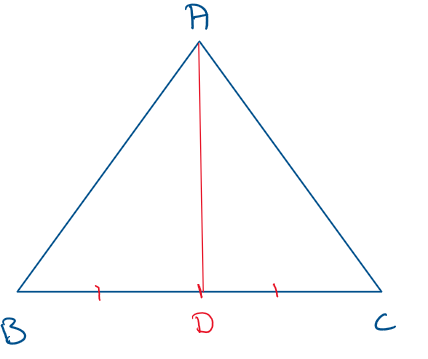
\includegraphics[width=0.25\linewidth]{Quant//Geometry//Images//Triangles/triangle_median_intro.png}
\end{figure*}


$AD$ is the median of side $BC$ and $BD = CD$. Note that \textbf{median is not necessarily a perpendicular to the side} 

A centroid is the intersection of all medians of a triangle. 

\begin{figure*}[h!]
    \centering
    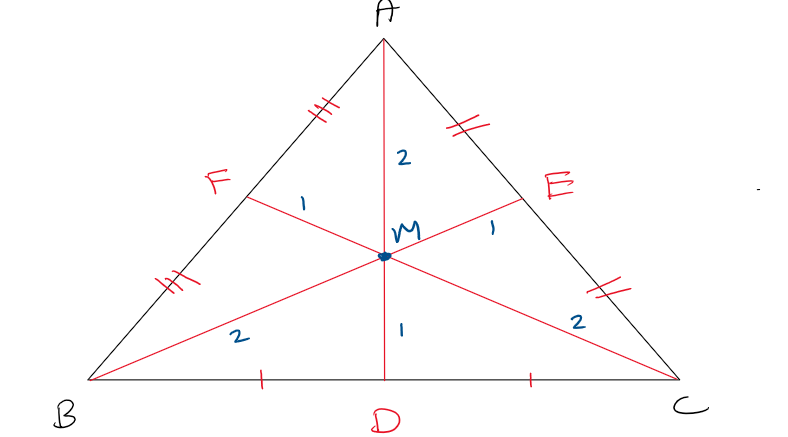
\includegraphics[width=0.4\linewidth]{Quant//Geometry//Images//Triangles/triangle_centroid_intro.png}    
\end{figure*}
        

A centroid divides the medians in the ratio of 2:1 from the vertex of median
\begin{itemize}
    \item $AM : MD = 2 : 1$
    \item $BM : ME = 2 : 1$
    \item $CM : MF = 2 : 1$
\end{itemize}
It divides the triangle into 6 triangles of equal area $\implies$ AMF = AME = BMF = BMD = CMD = CEF in terms of area

\subsection{Altitude and Orthocenter}
An altitude (perpendicular) is a vertical line from vertex to edge of a triangle. It makes an angle of 90 degree (right angle) with the base. \textbf{Perpendicular is not median}. As we can see, $AD$ is altitude (as it makes an angle of $\degree{90}$ with the base and $AM$ is the median. 

\begin{figure*}[h!]
    \centering
    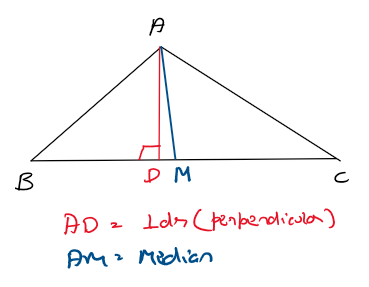
\includegraphics[width=0.5\linewidth]{Quant//Geometry//Images//Triangles/altitude.png}
\end{figure*}

Orthocenter of a triangle is the point of intersection of altitudes made from each vertex of triangle to its corresponding edge. In the figure below, $O$ is the orthocenter. 

\begin{figure*}[h!]
    \centering
    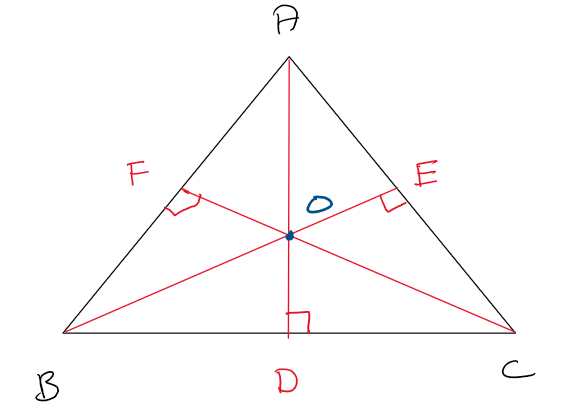
\includegraphics[width=0.5\linewidth]{Quant//Geometry//Images//Triangles/orthocenter.png}
\end{figure*}

A \textbf{property of orthocenter} : The sum of angles between two vertex and orthocentre and the angle of other vertex is always 180 degree. From this, we can say that in the above figure
\begin{itemize}
    \item $\angle A + \angle BOC = \degree{180}$
    \item $\angle B + \angle AOC = \degree{180}$
    \item $\angle C + \angle AOB = \degree{180}$
\end{itemize}

\subsection{Angle Bisector and Incenter}
Angle bisector is drawn from vertex of triangle to the adjacent side. This line divides the angle at the vertex in two equal angles

\begin{figure*}[h!]
    \centering
    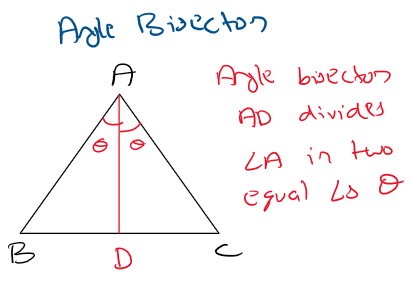
\includegraphics[width=0.5\linewidth]{Quant//Geometry//Images//Triangles/angle_bisector.png}
\end{figure*}

Incentre (Incenter) is the point at which the angle bisectors of each vertex of triangle intersect. This point is denoted as $I$. In the below figure, $AD, BE, CF$ are angle bisectors

\begin{figure*}[h!]
    \centering
    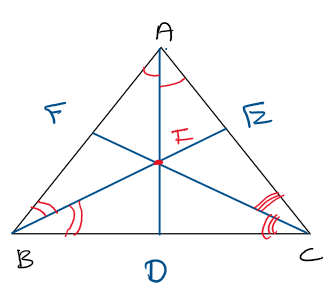
\includegraphics[width=0.5\linewidth]{Quant//Geometry//Images//Triangles/incenter.png}
\end{figure*}

\textbf{Property} : The angle made between an edge and incenter is related to the angle of the other vertex are as follows:
\begin{itemize}
    \item $\angle BIC = 90 + \dfrac{\angle A}{2}$
    \item $\angle AIC = 90 + \dfrac{\angle B}{2}$
    \item $\angle AIB = 90 + \dfrac{\angle C}{2}$
\end{itemize}

\subsection{Perpendicular Side Bisectors and Circumcenter}
Perpendicular Side Bisector is the line which divides a line in two equal parts at a right angle. In the triangle below, $DX$ is the perpendicular bisector of $BC$ which divides $BC$ into $BX \text{ and } CX \text{ where } BX = CX$

\begin{figure*}[h!]
    \centering
    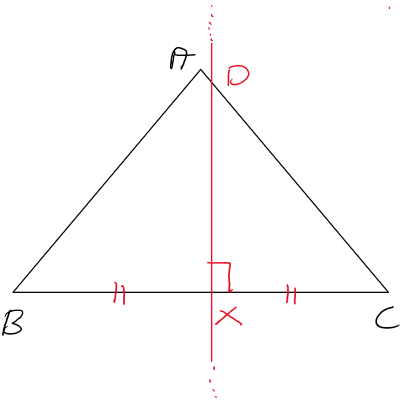
\includegraphics[width=0.5\linewidth]{Quant//Geometry//Images//Triangles/perpendicular_side_bisector.png}
\end{figure*}

Circumcenter is the point where perpendicular side bisectors of the three sides of a triangle intersect. In the triangle below, it is denoted as $O$

\begin{figure*}[h!]
    \centering
    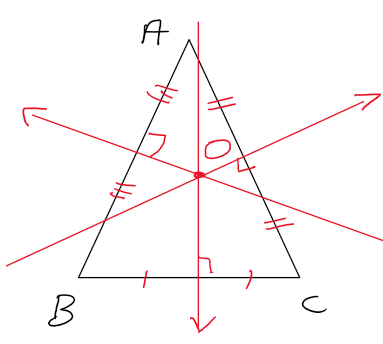
\includegraphics[width=0.5\linewidth]{Quant//Geometry//Images//Triangles/circumcenter.png}
\end{figure*}

\newpage

\subsection{Incircle and Circumcircle}

\subsubsection{Incircle}
We can make a circle inside a triangle by keeping the incenter as origin. This circle will intersect the triangle at three points. The radius of incircle is denoted by $r$. Note that in the below figure, $IX = IY = IZ = r$

\begin{figure*}[h!]
    \centering
    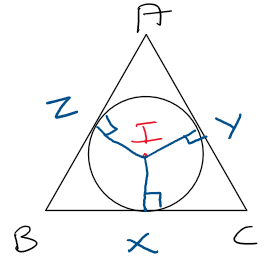
\includegraphics[width=0.4\linewidth]{Quant//Geometry//Images//Triangles/incircle.png}    
\end{figure*}

A circle's radius is perpendicular to its tangents. In this case
\begin{itemize}
    \item $IY$ is perpendicular to $AC$ ($AC$ is tangent)
    \item $IX$ is perpendicular to $BC$ ($BC$ is tangent)
    \item $IZ$ is perpendicular to $BA$ ($BA$ is tangent)
\end{itemize}

\subsubsection{Circumcircle}
We can draw a circle using this circumcenter. This circle will cover the full triangle. There is an interesting property : The circumcenter $O$ is equidistant from vertices of Triangle $\implies OA = OB = OC = R$

\begin{figure*}[h!]
    \centering
    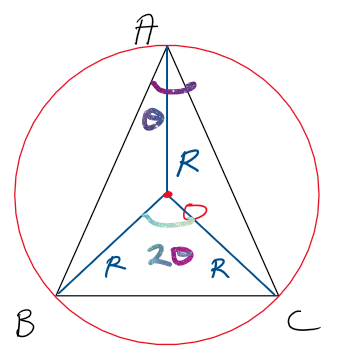
\includegraphics[width=0.38\linewidth]{Quant//Geometry//Images//Triangles/circumcircle.png}
\end{figure*}

This is a property of circles and sectors that is applicable to circumcircle..
$$
\angle BOC = 2 * \angle A
$$

\subsubsection{Distance between circumcenter and incenter}
The distance $d$ between Cirucmcenter with radius (called \textbf{circumradius}) $R$ and incenter with radius (called \textbf{inradius}) $r$ is defined as $d^2 = R * (R - 2r)$ \\

We can use the above formula to derive a relation between Inradius and circumradius as follows
\begin{align*}
    d^2 &\geq 0 \tag{Square of a number is always positive} \\
    R * (R - 2r) &\geq 0 \\
    R - 2r &\geq 0 \\
    \dfrac{R}{r} &\geq 2 \tag{$\dfrac{R}{r} = 2$ if triangle is equilateral}
\end{align*}

\SampleQuestion{In $\Triangle{ABC}$, $O$ is the point of intersection of altitudes and $I$ is the point of intersection of angle bisectors. If $\angle BOC = \degree{112}$, then find $\angle BIC$}

\begin{figure*}[h!]
    \centering
    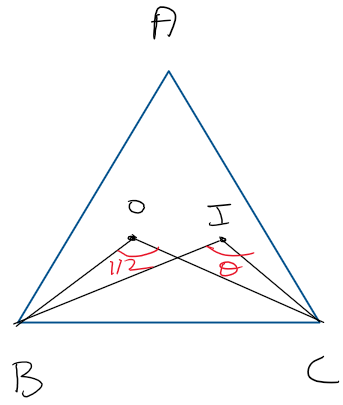
\includegraphics[width=0.3\linewidth]{Quant//Geometry//Images//Triangles/geo_center_question_1.png}
\end{figure*}

\begin{align*}
    \angle A + \angle BOC &= \degree{180} \tag{Property of orthocenter} \\
    \angle A &= \degree{68} \\
    \shortintertext{Now, using the above, we can find the value of $\angle BIC$} \\
    \angle BIC &= 90 + \dfrac{\angle A}{2} + 90 \tag{Property of incenter} \\
    &= \degree{124}
\end{align*}








\newpage

\section{Appollonius Theorem and Results}

\subsection*{Theorem}

This theorem is used to relate medians and triangles. The base theorem is that the median , the side on which we have drawn the median and the other sides of triangles are related

\begin{figure*}[h!]
    \centering
    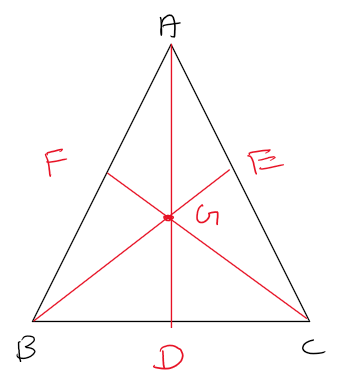
\includegraphics[width=0.3\linewidth]{Quant//Geometry//Images//Triangles/appollonius_figure.png}
\end{figure*}

For the above figure and medians, we have the following equations

\begin{table}[h!]
    \centering
    \begin{tabular}{|| c | c | c | c | p{3cm} ||}
        \hline
         Median & Base & Other Sides & Relation & Alternative \\
         \hline
         $AD$ & $BC$ & $AB,AC$ & $2 * (AD^2 + CD^2 ) = AB^2 + AC^2$ & Instead of $CD$, we can also use $BD$) \\
         \hline
         $BE$ & $AC$ & $AB,BC$ & $2 * (BE^2 + CE^2 ) = AB^2 + BC^2$ & Instead of $CE$, we can also use $AE$) \\
         \hline
         $CF$ & $AB$ & $AC,BC$ & $2 * (CF^2 + AF^2 ) = AC^2 + BC^2$ & Instead of $AF$, we can also use $BF$) \\
         \hline
    \end{tabular}
\end{table}

\subsection*{Results}

\begin{itemize}
    \item $\dfrac{\text{Sum of square of medians of triangle}}{\text{Sum of square of sides of triangle}} = \dfrac{3}{4}$

    \item Sum of medians $<$ Perimeter of Triangle $< \dfrac{4}{3}$ Sum of medians
    \item The centroid divides a median in the ratio $2 : 1$. For the sake of below formula, let us refer the sides as "bigger side" and "smaller side"... 
    $$
    \dfrac{ \text{Sum of square of bigger sides of median} }{ \text{Sum of square of sides of triangle} } = \dfrac{1}{3}
    $$
\end{itemize}

\newpage 

\section{Area of Triangle}
\subsection{Heron's Formula}

In the triangle with lengths of sides as $a,b,c$, we can find area using the formula below

\begin{figure*}[h!]
    \centering
    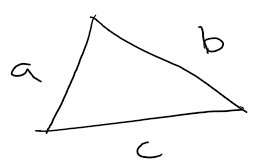
\includegraphics[width=0.4\linewidth]{Quant//Geometry//Images//Triangles/herons.png}
\end{figure*}

Area = $\sqrt{ s * (s - a) * (s - b) * (s - c) }$, $s = \dfrac{a + b + c}{2}$

\subsection{Using base and height}

The formula is $\dfrac{1}{2} * \text{base} * \text{height}$. The important thing is to determine correctly which dimension is the base and which is the height. 

\begin{figure*}[h!]
    \centering
    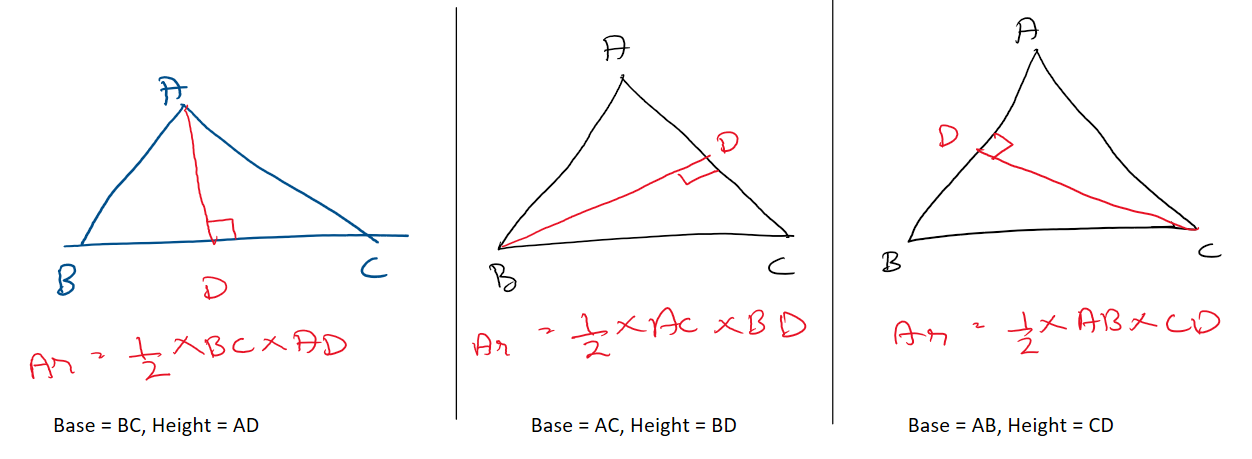
\includegraphics[width=1.0\linewidth]{Quant//Geometry//Images//Triangles/half_base_height.png}
\end{figure*}


\subsection{Using Inradius and Circumradius}

For a triangle with dimensions as $a,b,c$, its area with respect to incenter and circumcenter is summarised in below table

\begin{table}[h!]
    \centering
    \begin{tabular}{|| c | c | c | c ||}
        \hline
         Radius & Represented as & Formula & Note \\
        \hline
         Inradius & $r$ & $r * s$ & $s = \dfrac{a + b + c}{2}$ \\
        \hline
         Circumradius & $R$ & $\dfrac{abc}{4R}$ & \\
        \hline
    \end{tabular}
\end{table}

\subsection{Using Trigonometery}
We can also using trigonometery to calculate area of triangle. We will consider any two sides of triangle and the angle between them. 

\begin{figure*}[h!]
    \centering
    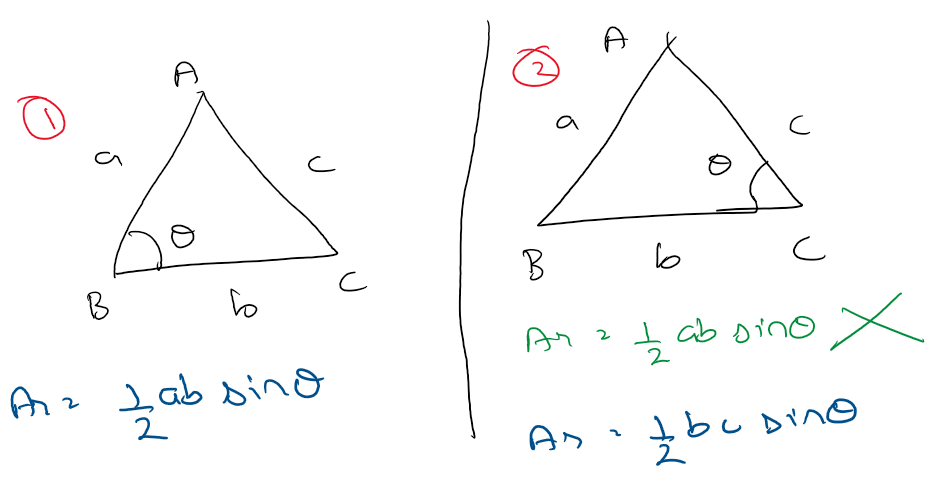
\includegraphics[width=0.9\linewidth]{Quant//Geometry//Images//Triangles/area_trigo.png}
\end{figure*}

\begin{itemize}
    \item In case 1, the angle $\theta$ between sides $a$ and $b$ is considered. The area is $\dfrac{1}{2} * a * b * \sin{\theta} $

    \item In case 2, the angle $\theta$ between sides $b$ and $C$ \textbf{should be considered.} . The area is $\dfrac{1}{2} * b * c * \sin{\theta} $
    
\end{itemize}


\subsection{Area of triangle made by median}
For a triangle ABC, when the length of the medians $AD, BE, CF$ are given, then if we arrange the medians in such a way that they make a triangle DEF, then area of ABC and DEF are related as follows

$$
\Area{DEF} = \dfrac{3}{4} \Area{ABC}
$$

\SampleQuestion{$AD = 9, BE = 12, CF = 15$. $AD,BE \& CF$ are medians of $\Delta ABC$. Find the area of $\Delta ABC$}

\begin{figure*}[h!]
    \centering
    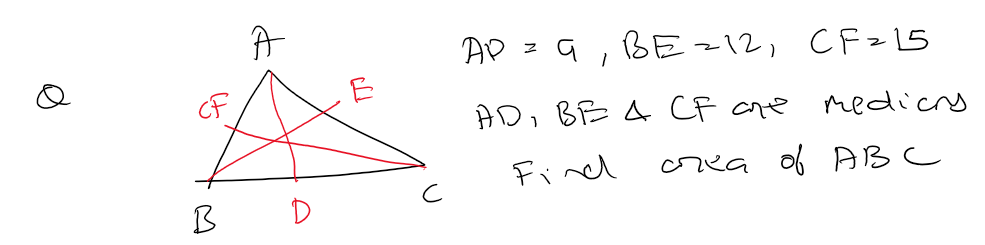
\includegraphics[width=0.7\linewidth]{Quant//Geometry//Images//Triangles/area_of_triangle_question_1.png}
\end{figure*}

We will arrange the medians in a triangle and apply the above theorem. First, let us see which sides of triangle satisfy the pythagoreas theorem or not
\begin{align*}
    15^2 = 9^2 + 12^2
\end{align*}

Based on this, this is how the triangle will look like
\begin{figure*}[h!]
    \centering
    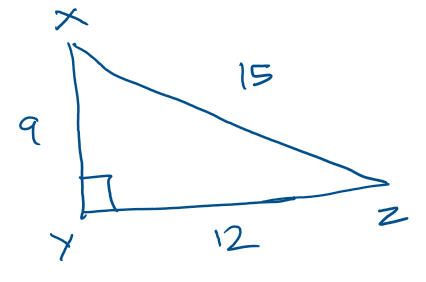
\includegraphics[width=0.5\linewidth]{Quant//Geometry//Images//Triangles/area_of_triangle_question_1_solution.png}
\end{figure*}

\begin{itemize}
    \item Area ($\Delta XYZ$) = $\dfrac{1}{2} * 9 * 12 = 54$. 
    \item Area ($\Delta ABC$) = $\dfrac{3}{4} * 54 = 72$. 
\end{itemize}

\SampleQuestion{Find AD in the following figure}

\begin{figure*}[h!]
    \centering
    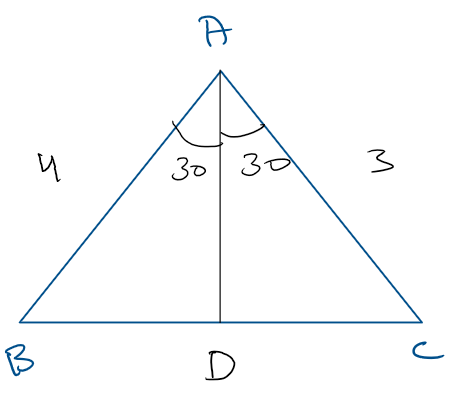
\includegraphics[width=0.40\linewidth]{Quant//Geometry//Images//Triangles/area_of_triangle_question_2.png}
\end{figure*}

Area of ABC 
\begin{itemize}
    \item Using trigonometry : $\dfrac{1}{2} * 4 * 3 * \sin{60} = 3 \sqrt{3}$
    \item In terms of smaller triangles : $\Area{ABC} = \Area{ABD} + \Area{ACD}$
\end{itemize}

\begin{align*}
    \Area{ABC} &= \bigParen{\dfrac{1}{2} * 4 * AD * \sin{30}} +  \bigParen{\dfrac{1}{2} * 3 * AD * \sin{30}} \\
    3 \sqrt{3} &= \dfrac{1}{4} * \bigParen{4 * AD + 3 * AD} \tag{$\sin{30} = \frac{1}{2} $} \\
    12 \sqrt{3} &= 7 * AD \\
    AD &= \dfrac{12 \sqrt{3}}{7}
\end{align*}

\SampleQuestion{A semicircle is inside a triangle with its origin on the side $BC$ as shown below .Find the radius $r$ of the semicircle}

\begin{figure*}[h!]
    \centering
    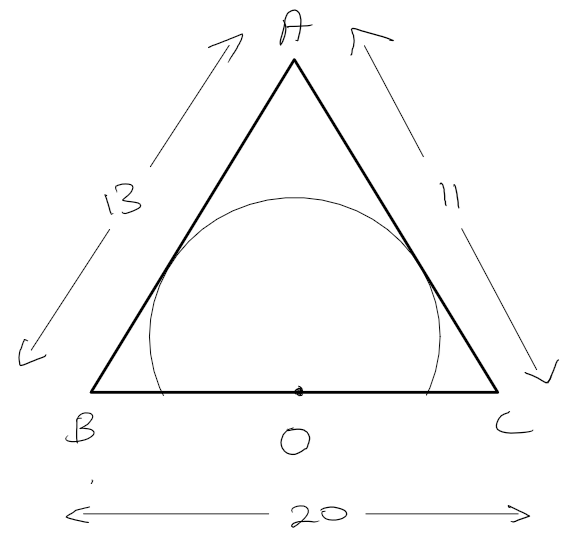
\includegraphics[width=0.4\linewidth]{Quant//Geometry//Images//Triangles/area_of_triangle_question_3.png}
\end{figure*}

We need to find $r$ as shown in the above figure. To do so, we can equate area of $\Triangle ABC$ with area of triangles $\Triangle AOB$ and $\Triangle AOC$. We can see that $ \Area{ABC} = \Area{AOB} + \Area{AOC} $

\begin{figure*}[h!]
    \centering
    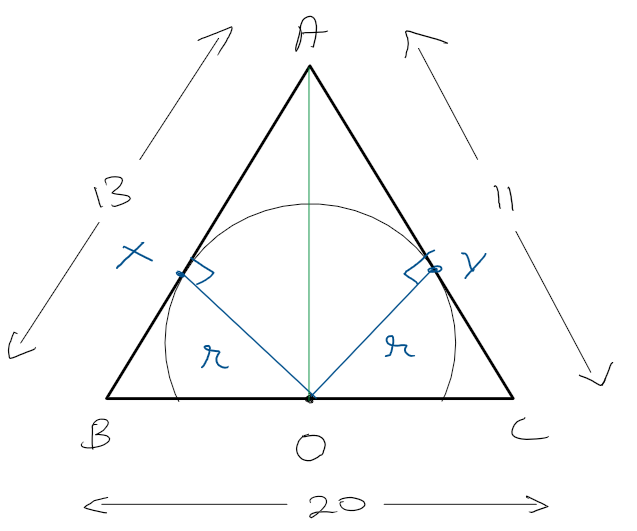
\includegraphics[width=0.5\linewidth]{Quant//Geometry//Images//Triangles/area_of_triangle_question_4_sol_fig.png}
\end{figure*}

\textbf{Calculating $\Area{ABC}$}
$s = \dfrac{13 + 11 + 20}{2} = 22$

\begin{align*}
    \Area{ABC} &= \sqrt{s * (s - a) * (s - b) * (s - c)} \\
    &= \sqrt{22 * (22 - 13) * (22 - 20) * (22 - 11)} \\
    &= \sqrt{22 * 9 * 2 * 11} \\
    &= \sqrt{2 * 11 * 3 * 3 * 2 * 11} \\
    &= 66
\end{align*}

\textbf{Calculating $\Area{ABO}$}
Base = 13, Height = $OB = r$
\begin{align*}
    \Area{ABO} &= \dfrac{1}{2} * 13 * r
\end{align*}

\textbf{Calculating $\Area{ACO}$}
Base = 11, Height = $OC = r$
\begin{align*}
    \Area{ABO} &= \dfrac{1}{2} * 11 * r
\end{align*}

\textbf{Equating Areas}
\begin{align*}
    \Area{ABC} &= \Area{AOB} + \Area{AOC} \\
    66 &= \dfrac{1}{2} * (13r + 11r) \\
    r &= \dfrac{2 * 66}{24} \\
    r &= 5.5
\end{align*}

\SampleQuestion{In $\Triangle ABC$, $AB = 17.5, AC = 9.$ Let $D$ be a point on BC such that AD is perpendicular to BC. If $AD = 3$ then what is the radius of the circle circumscribing $\Triangle ABC$ ?}

\begin{figure*}[h!]
    \centering
    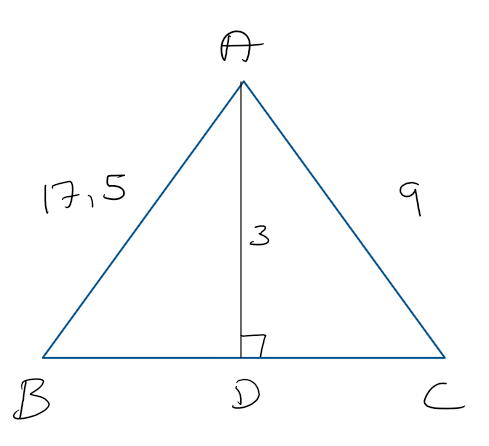
\includegraphics[width=0.4\linewidth]{Quant//Geometry//Images//Triangles/geo_center_question_2.png}
\end{figure*}

\begin{itemize}
    \item Area of triangle using Circumradius = $\dfrac{AB * AC * BC}{4 * R}$
    \item Area of triangle using base and height = $\dfrac{1}{2} * BC *  AD$
\end{itemize}

Using the above 
\begin{align*}
    \dfrac{AB * AC * BC}{4 * R} &= \dfrac{1}{2} * BC *  AD \\
    R &= \dfrac{AB * AC * BC * 2}{4 * BC * AD} \\
    &= \dfrac{17.5 * 9 * 2}{4 * 3} \tag{Removed BC as it is common} \\
    &= 26.25
\end{align*}







\newpage
\section{Angle Bisector Theorem}
An angle bisector divides the base in the ratio of the other sides of triangle. This is true for both internal and external angle bisectors

\begin{figure*}[h!]
    \centering
    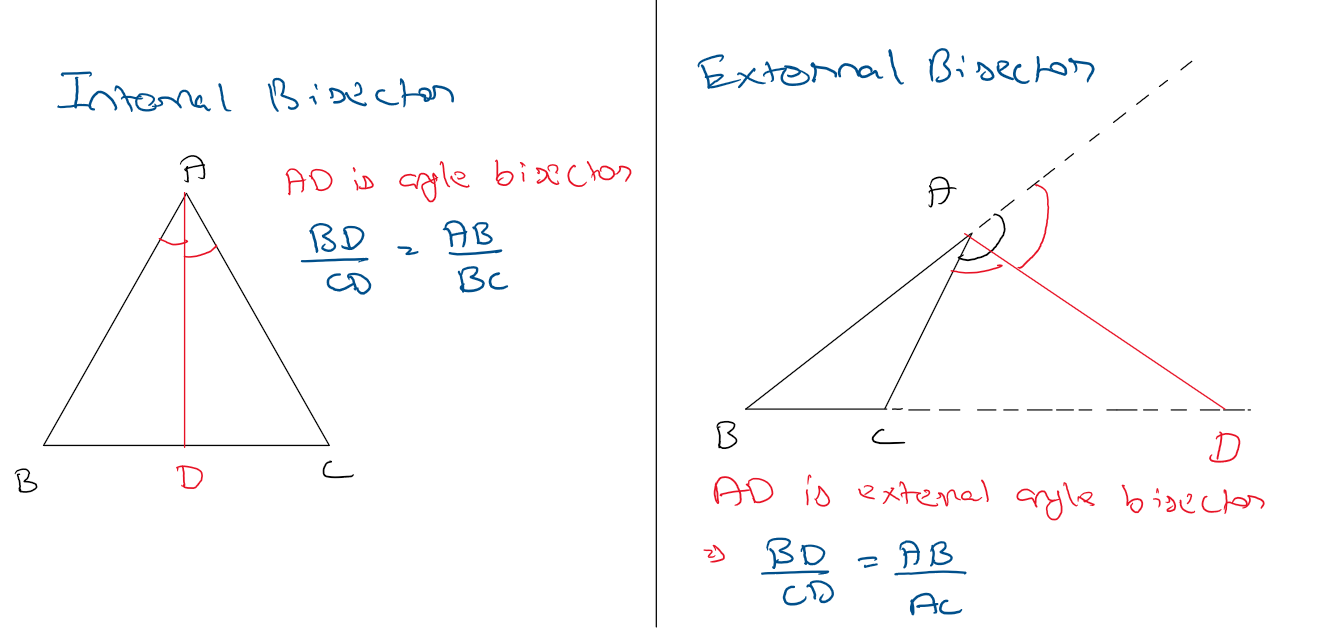
\includegraphics[width=1.02\linewidth]{Quant//Geometry//Images//Triangles/angle_bisector_theorem.png}
\end{figure*}

In the external angle bisector case, we "extended" $BC$ and determined a point $D$ at which $AD$ will divide the exterior $\angle A$ in two equal parts. The partitions created by point $D$ are still $BD$ and $CD$ (even though visually, it looks like $C$ divides $BD$)





























\newpage

\section{Right Triangles}
\subsection{Orthocenter and Circumcenter}
A right triangle is a triangle where one side has right angle. 

\begin{figure*}[h!]
    \centering
    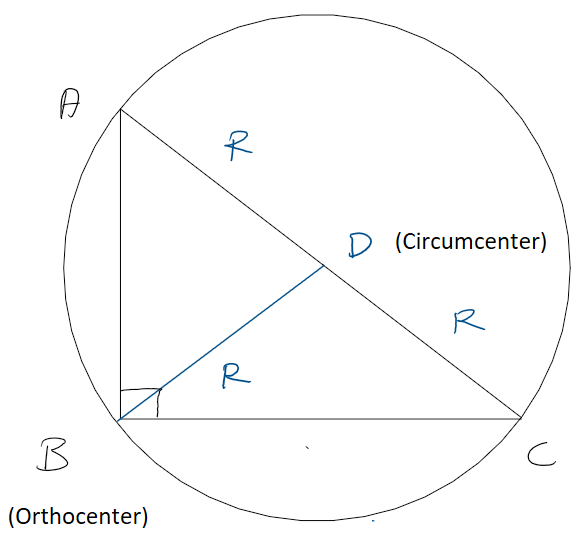
\includegraphics[width=0.5\linewidth]{Quant//Geometry//Images//Triangles/rt_triangle_ortho_circumcenter.png}
\end{figure*}

In the figure above, there are few interesting properties about right triangle
\begin{itemize}
    \item Circumcenter is midpoint of hypotenuse (Point $D$)
    \item Orthocenter is the vertex where the $\degree{90}$ is present (Point $B$)
    \item The line joining orthocenter and circumcenter is median of triangle with the length $R = $ circumradius. ($BD = AD = CD$)
    \item Circumradius of triangle is $\dfrac{1}{2} * \text{ hypotenuse } $ ($\dfrac{AC}{2}$)
\end{itemize}

\newpage

\subsection{Incircle in terms of Hypotenuse}
Before we explore this, we should know this property of circles : \textbf{Two tangents drawn from same point to a circle are equal}. In the below figure, from $P$ we have drawn two tangents $PA$ and $PB$ to circle. According to above property, $PA = PB$

\begin{figure*}[h!]
    \centering
    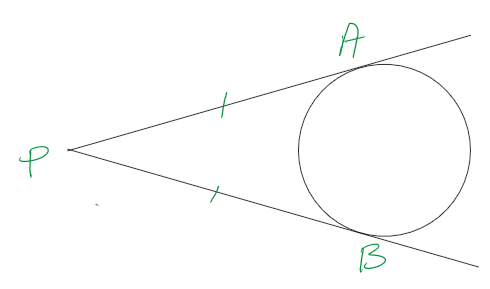
\includegraphics[width=0.4\linewidth]{Quant//Geometry//Images//Triangles/two_tangents_from_same_pt_circle.png}
\end{figure*}

Using this, we can prove that Inradius $r$ of a right triangle is given as 

\begin{align*}
    r &= s - h \tag{$ s = \dfrac{a + b + c}{2} $} \\
    \tag{$h = \text{hypotenuse}$}
\end{align*}

Let us try to derive this. Let us refer the example below. In the below figure, we have $\Triangle ABC$ where the circle inscribed inside the triangle has its origin on incenter. Therefore, $r$ represents inradius.

\begin{figure*}[h!]
    \centering
    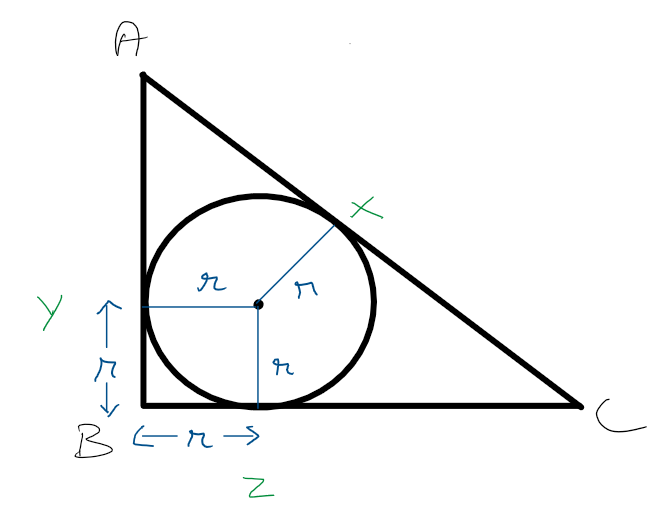
\includegraphics[width=0.5\linewidth]{Quant//Geometry//Images//Triangles/rt_triangle_inradius_hypo_theory.png}
\end{figure*}

In this triangle, $AB = c, BC = a, AC = b$. Using the property we discussed above for circles and tangents, we can say the following things
\begin{itemize}
    \item  $CZ = a - r, CX = a - r$ (Tangent from point $C$)
    \item  $AY = c - r, AX = c - r$ (Tangent from point $A$)
\end{itemize}

Hypotenuse is defined by $b$. We can see that
\begin{align*}
    b &= (a - r) + (c - r) \\
    2r &= a + c - b \\
    r &= \dfrac{a + c - b}{2} \\
    r &= \dfrac{a + b + c}{2} - b \tag{If you solve this, it will give the original expression back} \\
    r &= s - h \tag{$s = \dfrac{a + b + c}{2}, h = $ hypotenuse}
\end{align*}

\subsection{Pythagorean Triplets}
A group of 3 numbers which satisfies the pythagorean theorem. Some of the basic triplets are as follows (\textbf{memorise them})
\begin{enumerate}
    \item 3,4,5 ($5^2 = 3^2 + 4^2$)
    \item 5,12,13 ($13^2 = 5^2 + 12^2$)
    \item 7,24,25 ($25^2 = 7^2 + 24^2$)
    \item 8,15,17 ($17^2 = 8^2 + 15^2$)
    \item 9,40,41 ($41^2 = 9^2 + 40^2$)
    \item 20,21,29 ($29^2 = 20^2 + 21^2$)
\end{enumerate}

\SampleQuestion{Can we create a right triangle with sides of length 18,24,30 ?}

$18,24,30 = 6 * 3, 6 * 4, 6 * 5$. Taking 6 common, we will have $(3,4,5)$. Since this is a multiple of the basic pythagorean triplet we listed above, we can create a right triangle with these dimensions

\SampleQuestion{Find area of triangle with sides of length 15, 36, 39}

$15, 36, 39 = 3 * 5, 3 * 12, 3 * 13$. Taking 3 common, we will have $(5,12,13)$. Since this is a multiple of the basic pythagorean triplet we listed above, we can create a right triangle with these dimensions. The right triangle will have 
\begin{itemize}
    \item Base = 12
    \item Height = 5
    \item Hypotenuse = 13
\end{itemize}

Area = $\dfrac{1}{2} * 5 * 12 = 30$. Now, area of original triangle = $9 * 30 = 270$. We multiply with 9 (instead of 3) because area of triangle is defined as $\dfrac{1}{2} * b * p$. Now, in this question, $b = 3 * 5, p = 3 * 12$. We can see that the constant $3$ is multiplied twice

\subsection{Formation of pythagorean triplets}
Let us assume we have three numbers $(a,b,c)$. To form a pythagorean triplet, we have the following conditions

\subsubsection{Odd Values}
\begin{itemize}
    \item $\dfrac{b + c}{2} = \dfrac{a^2}{2}$
    \item $b$ and $c$ will be consecutive numbers
\end{itemize}

\begin{table}[h!]
    \centering
    \begin{tabular}{|| c | c | c | c ||}
        \hline
         \textbf{Triplet} & \textbf{a} & $\dfrac{a^2}{2}$ & $\dfrac{b + c}{2}$  \\
        \hline
         (3,4,5) & 3 & 4.5 & $\dfrac{4 + 5}{2} = 4.5 $ \\
        \hline
         (5,12,13) & 5 & 12.5 & $\dfrac{12 + 13}{2} = 12.5 $ \\
        \hline
         (11,60,61) & 5 & 60.5 & $\dfrac{60 + 61}{2} = 60.5 $ \\
        \hline
         (11,60,61) & 5 & 60.5 & $\dfrac{60 + 61}{2} = 60.5 $ \\
        \hline
    \end{tabular}
\end{table}

\subsubsection{Even Values}
\begin{itemize}
    \item $\dfrac{b + c}{2} = \dfrac{a^2}{4}$
    \item $b$ and $c$ will have difference of 2
\end{itemize}

\begin{table}[h!]
    \centering
    \begin{tabular}{|| c | c | c | c ||}
        \hline
         \textbf{Triplet} & \textbf{a} & $\frac{a^2}{4}$ & $\frac{b + c}{2}$  \\
        \hline
         (4,3,5) & 4 & 4 & $\dfrac{3 + 5}{2} = 4 $ \\
        \hline
         (8,15,17) & 8 & 16 & $\dfrac{15 + 17}{2} = 16 $ \\
        \hline
         (12,35,37) & 12 & 36 & $\dfrac{35 + 37}{2} = 36 $ \\
        \hline
    \end{tabular}
\end{table}

\SampleQuestion{Find sum of inradius of $\Triangle{ABD}$ and $\Triangle{ADC}$}

\begin{figure*}[h!]
    \centering
    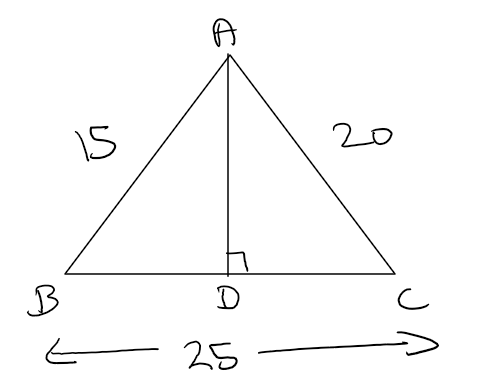
\includegraphics[width=0.4\linewidth]{Quant//Geometry//Images//Triangles/rodha_triangle_5_q1.png}
\end{figure*}

In a right triangle, inradius is defined as difference of $s$ and $h$ where $s = \dfrac{a + b + c}{2}$ and $h = \text{hypotenuse}$. To calculate inradius for the two triangles, we need to find $AD$ and the bases of their triangles

\vspace{1cm}

\textbf{Finding AD}
\begin{itemize}
    \item We will calculate area of ABC and then use $\dfrac{1}{2} * \text{base} * \text{height}$ formula where base = BC, height = AD
    
    \item $s = \dfrac{a + b + c}{2} \implies \dfrac{15 + 20 + 25}{2} = 30$

    \item $\Area{ABC} = \sqrt{30 * (30 - 15) * (30 - 20) * (30 - 25)} \implies \sqrt{30 * 15 * 20 * 25} = 150$

    \item Using base and height, $\Area{ABC} = \dfrac{1}{2} * 25 * AD \implies 150 = \dfrac{1}{2} * 25 * AD \implies AD = 12$
\end{itemize}

\vspace{1cm}

$\Triangle{ABD}$ \\
Using pythagoreas theorem, we can find value of $BD$ 
\begin{align*}
    AB^2 &= AD^2 + BD^2 \\ 
    BD &= \sqrt{AB^2 - AD^2} \\
    &= \sqrt{15^2 - 12^2} \\
    &= \sqrt{27 * 3} \\
    &= 9
\end{align*}

Inradius of $\Triangle{ABD}$
\begin{align*}
    r_{ABD} &= s_{ABD} - h_{ABD} \\
    &= \dfrac{15 + 12 + 9}{2} - 15 \\
    &= 18 - 15 = 3
\end{align*}

\vspace{1cm}

$\Triangle{ADC}$ \\
We know that $BD = 9 \implies DC = 16$. We can find $r_{ABD}$ as 
\begin{align*}
    r_{ABD} &= s_{ABD} - h_{ABD} \\
    &= \dfrac{20 + 16 + 12}{2} - 20 \\
    &= 24 - 20 = 4
\end{align*}

\textbf{Sum of inradius = } 7


\newpage

\SampleQuestion{ABCD is a rectangle with DC = 12 and BC = 9. Find the distance between incenters of $\Triangle{ADC}$ and $\Triangle{ABC}$}

\begin{figure*}[h!]
    \centering
    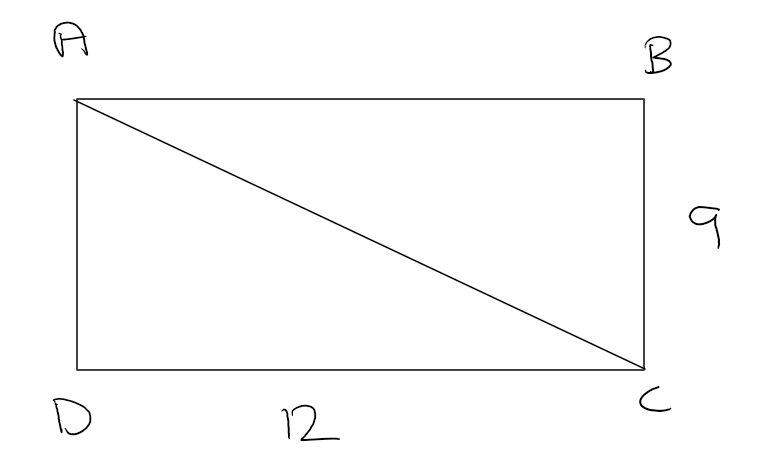
\includegraphics[width=0.5\linewidth]{Quant//Geometry//Images//Triangles/rodha_triangle_5_q2_1.png}
\end{figure*}

In the rectangle, $\angle{D} = \angle{B} = \degree{90}$. We can find AC as $AC^2 = AD^2 + DC^2 \implies AC = 15$. Using the formula $r = s - h$ to find inradius, we can find inradius of both triangles as follows
\begin{itemize}
    \item For both triangles, $s = \dfrac{12 + 15 + 9}{2} = 18$
    \item $\Triangle{ADC}$ : 18 - 15 = 3
    \item $\Triangle{ABC}$ : 18 - 15 = 3
\end{itemize}

Now, look at the diagram below. We see that we can form a triangle where $r_1 \text{and} r_2$ are the hypotenuse of a triangle with base = 6 and height = 3 (triangle created by red color). 

\begin{figure*}[h!]
    \centering
    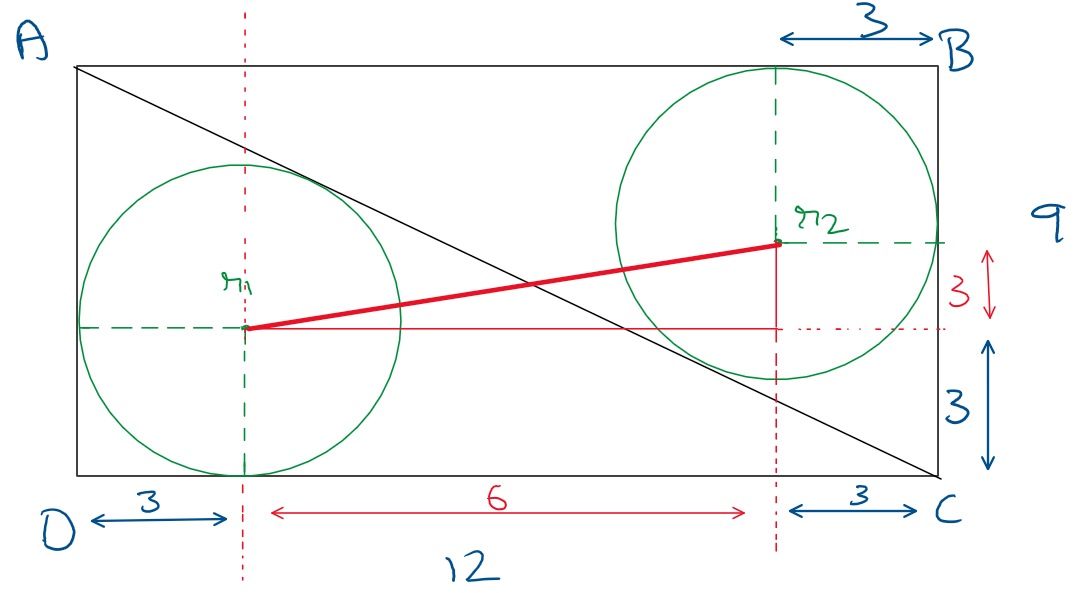
\includegraphics[width=0.7\linewidth]{Quant//Geometry//Images//Triangles/rodha_triangle_5_q2_2.png}
\end{figure*}

Distance between incenters = $\sqrt{6^2 + 3^2} \implies \sqrt{45} = 3 \sqrt{5}$

\newpage

\SampleQuestion{In a right triangle, area = 80 and perimeter = 80. Find the length of the hypotenuse}

We can write the area of a triangle in terms of its perimeter (semiperimeter $s$) as $r * s$ where $r = \text{Inradius}$. In a right triangle, $r = s - h$ where $h = \text{hypotenuse}$. Using these, we can find our values
\begin{itemize}
    \item $s = \dfrac{p}{2} \implies \dfrac{80}{2} = 40$
    \item Finding $r$ through area : $80 = r * 40 \implies r = 2$
    \item Finding $h$ through $r$ : $r = s - h \implies h = s - r \implies h = 38$
\end{itemize}

\SampleQuestion{What is the area of a right triangle with R (circumradius) = 18 and r (inradius) = 8 ?}

\begin{itemize}
    \item In a right triangle, $R = \frac{h}{2}$ where $h = hypotenuse$. From above, we can get $h = 36$

    \item In a right triangle, $r = s - h \implies s = 8 + 36 = 44$

    \item Area = $r * s = 8 * 44 = 352$
\end{itemize}

\SampleQuestion{In a right triangle, $a,b,c$ are sides of traingles where $c > b > a$. Also, we are given that $a = 12$ and $2a + 7c = 9b$. Find the value of $c$}

\textbf{THIS IS A MIND BOGGLING QUESTION. TRY TO UNDERSTAND THE APPROACH BECAUSE IT IS NOT INTUITIVE}

We will be using the concept of pythagorean triplets in this one. Let us the equation to arrive at an interesting result

\begin{align*}
    2a + 7c &= 9b \\
    2a + 7c &= 2b + 7b \\
    2 * (a - b) &= 7 * (b - c) \\
    \dfrac{a - b}{b - c} &= \dfrac{7}{2}
\end{align*}

We came to a ratio where $a - b = 7$ and $b - c = 2$. Let us do hit and trial on the common pythagorean triplets
\begin{itemize}
    \item 3,4,5 : 4-3 = 1 REJECTED
    \item 5,12,13 : 12 - 5 = 7, 13 - 12 = 1 REJECTED
    \item 7,24,25 : 24 - 7 = 17 REJECTED
    \item 8,15,17 : 15 - 8 = 7, 17 - 15 = 2 ACCEPTED
\end{itemize}

Now, our first term of triplet is 12. To be of the form 8,15,17, we need to find the coefficient $\implies k = \dfrac{12}{8} = 1.5$. The triplet is, therefore $(12, 1.5 * 15, 1.5 * 17) = (12,22.5,25.5)$








\newpage

\section{Similarity of Triangles}

\hl{(WRITING THE THEORY PART ONLY. MAKE DIAGRAMS AND OTHER STUFF ON WEEKDAYS ALSO, FINISH ABOVE FIRST)}

Similarity is between two triangles. When two triangles are similar, we have the following properties
\begin{itemize}
    \item Ratio of corresponding sides are equal
    \item Ratio of corresponding sides = Ratio of Heights = Ratio of medians = Ratio of inradius = Ratio of circumradius
    \item Ratio of area = square of ratio of heights
\end{itemize}





\subsection{Types of similarity}

\subsubsection{SSS : Side, Side, Side}
Sides of two triangles are in same ratio. $\dfrac{AB}{PQ} = \dfrac{BC}{QR} = \dfrac{AC}{PR}$


\begin{figure*}[h!]
    \centering
    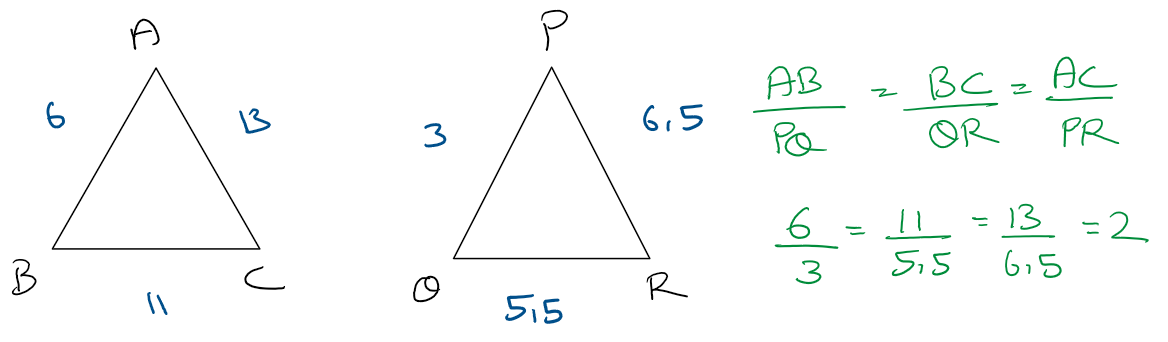
\includegraphics[width=0.8\linewidth]{Quant//Geometry//Images//Triangles/rodha_triangle_6_sss.png}
\end{figure*}

\subsubsection{AA : Angle, Angle}
Two angles . $\angle ADE = \angle ABC, \angle AED = \angle ACB$

\begin{figure*}[h!]
    \centering
    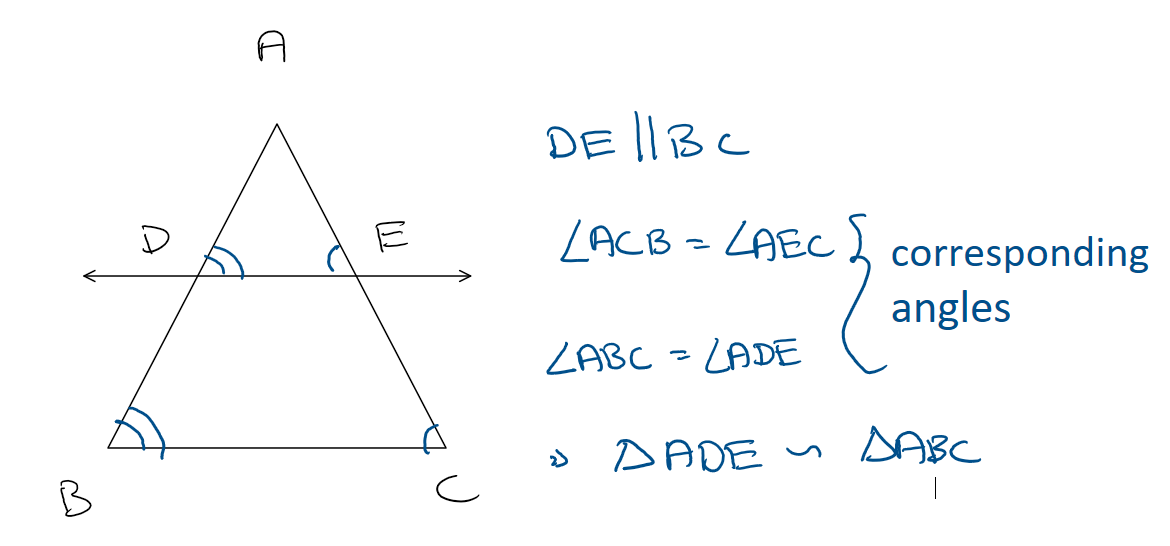
\includegraphics[width=0.9\linewidth]{Quant//Geometry//Images//Triangles/rodha_triangle_6_aa.png}
\end{figure*}

\subsubsection{SAS : Side, Angle, Side}

\begin{figure}[h!]
    \centering
    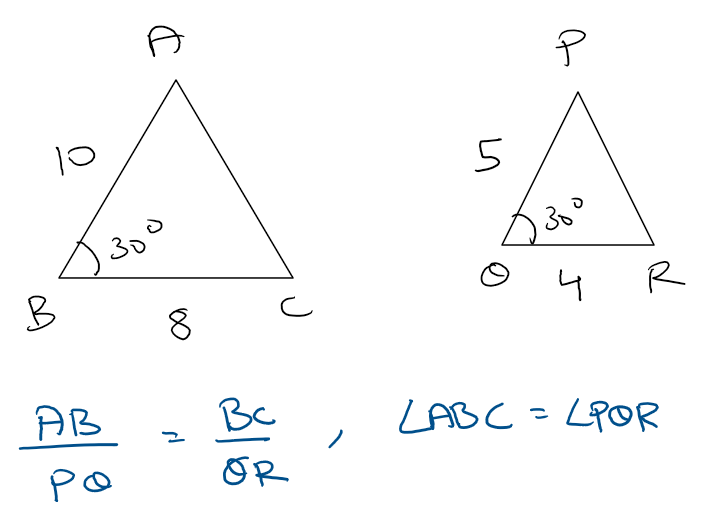
\includegraphics[width=0.5\linewidth]{Quant//Geometry//Images//Triangles/rodha_triangle_6_sas.png}
\end{figure}

\textbf{The angle must be between the two sides}. Ratio of two sides and the included angle is equal. $\dfrac{AB}{PQ} = \dfrac{BC}{QR}, \angle ABC = \angle PQR$. In this, $\angle ABC$ and $\angle PQR$ lie between AB and PQ respectively





\subsection{Determining How to find the sides / angles which should be similar}

Let us explore this using two cases

\subsubsection{CASE 1}

Let us say that we are given the following triangle and we need to find whether $\Triangle{ABC}$ is similar to $\Triangle{AXY}$ or not. In this triangle, XYZW is a rectangle that is inscribed inside the triangle

\begin{figure}[h!]
    \centering
    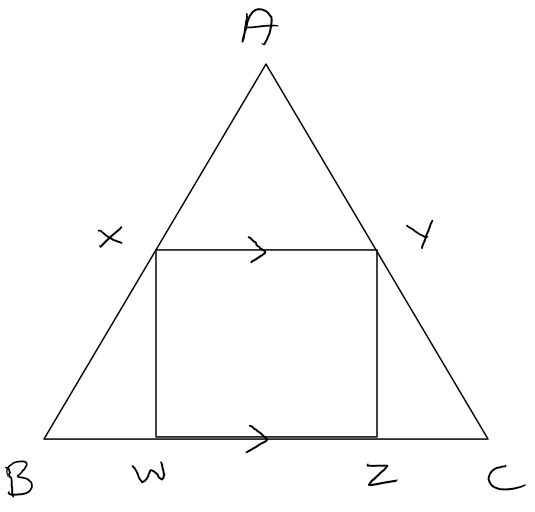
\includegraphics[width=0.5\linewidth]{Quant//Geometry//Images//Triangles/rodha_triangle_6_similarity_equation_case_1.png}
\end{figure}

We know that sides of a rectangle are parallel to each other. Using this, we can make some relations between the angles. In the below figure, we have marked $\angle{ABC} \text{ and } \angle{ACB} \text{ as } \theta \text{ and } \phi$ respectively. Using corresponding angles, $\angle{AXY} = \angle{ABC}$ and $\angle{AYX} = \angle{ACB}$. 

\begin{figure}
    \centering
    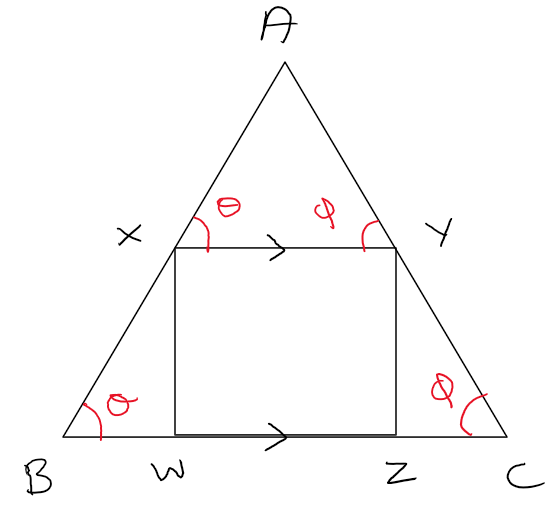
\includegraphics[width=0.5\linewidth]{Quant//Geometry//Images//Triangles/rodha_triangle_6_similarity_equation_case_1_2.png}
\end{figure}

We can now check for similarity between $\Triangle{AXY} \text{and} \Triangle{ABC}$
\begin{itemize}
    \item $\angle{AXY} = \angle{ABC}$
    \item $\angle{AYX} = \angle{ACB}$
    \item Hence proved similar through AA condition
\end{itemize}

To write the ratio of the sides, we will take the help of angles
\begin{table}[h!]
    \centering
    \begin{tabular}{|| c | c | c | c | c ||}
        \hline
         Angle in $\Triangle{AXY}$ & Side & Angle in $\Triangle{ABC}$ & Side & Ratio  \\
        \hline
         $\angle{AXY}$ & AY & $\angle{ABC}$ & AC & $\dfrac{AY}{AC}$ \\ 
         \hline
         $\angle{AYX}$ & AX & $\angle{ACB}$ & AB & $\dfrac{AX}{AB}$ \\ 
         \hline
         $\angle{XAY}$ & XY & $\angle{BAC}$ & BC & $\dfrac{XY}{BC}$ \\ 
         \hline
    \end{tabular}
\end{table}

\begin{NOTE}
    An interesting observation is in the notation of how we right angles. When we write an angle, say $\angle{ABC}$, $B$ is the part where the angle "exists" and $A$ and $C$ are the points that make that angle possible. In $\Triangle{ABC}$ , $\angle{ABC}$ is formed through the edge $AC$. This is a useful observation in writing similarity ratios
\end{NOTE}

\subsubsection{CASE 2}

This is an interesting case where we have a right triangle as follows

\begin{figure}[h!]
    \centering
    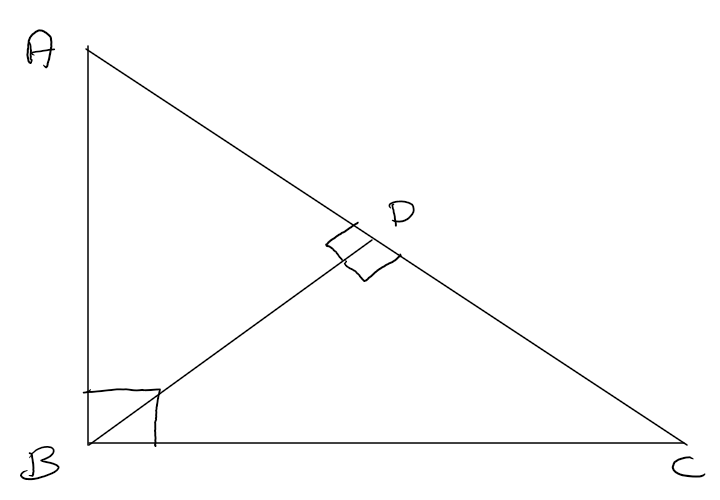
\includegraphics[width=0.5\linewidth]{Quant//Geometry//Images//Triangles/rodha_triangle_6_similarity_equation_case_2.png}
\end{figure}

In this triangle, we need to find whether the following triangles are similar or not

\begin{itemize}
    \item $\Triangle{ABD}$ and $\Triangle{CBD}$
    \item $\Triangle{ABC}$ and $\Triangle{ABD}$
    \item $\Triangle{ABC}$ and $\Triangle{CBD}$
\end{itemize}

\textbf{ First, let's start with $\Triangle{ABD}$ and $\Triangle{CBD}$ }

Let us assume that $\angle{ACB} = \theta$

In $\Triangle{BCD}$
\begin{align*}
    \angle{DBC} + \angle{BDC} + \angle{DCB} &= \degree{180} \tag{Angle sum property of triangle} \\
    \angle{DBC} + 90 + \theta &= \degree{180} \\
    \angle{DBC} &= 90 - \theta
\end{align*}

Now, we can see that $\angle{ABC} = \angle{ABD} + \angle{DBC} = \degree{90} \implies \angle{ABD} = \theta$

In $\Triangle{ABD}$
\begin{align*}
    \angle{BAD} + \angle{ADB} + \angle{DBA} &= \degree{180} \tag{Angle sum property of triangle} \\
    \angle{BAD} + 90 + \theta &= \degree{180} \\
    \angle{BAD} &= 90 - \theta
\end{align*}

We get a figure like this in the end

\begin{figure}[h!]
    \centering
    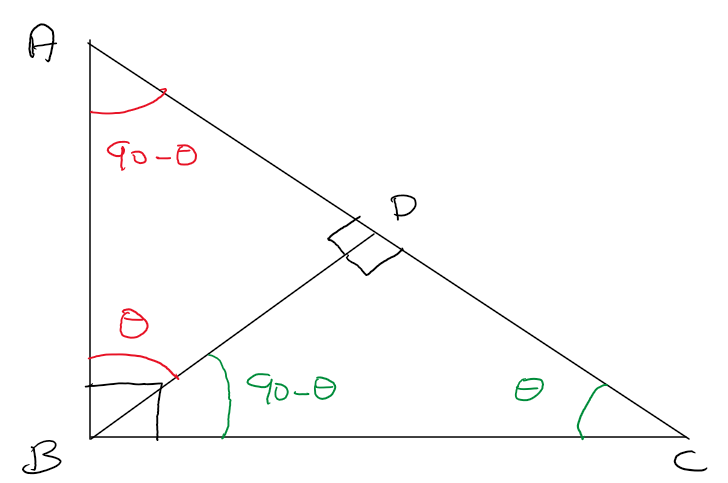
\includegraphics[width=0.5\linewidth]{Quant//Geometry//Images//Triangles/rodha_triangle_6_similarity_equation_case_2_2.png}
\end{figure}

We can find simlarity between $\Triangle{ABD}$ and $\Triangle{CBD}$ as follows
\begin{itemize}
    \item $\angle{DCB} = \angle{DBA}$
    \item $\angle{DBC} = \angle{DAB}$
    \item Hence similar by AA condition
\end{itemize}

To write the ratio of the sides, we will take the help of angles
\begin{table}[h!]
    \centering
    \begin{tabular}{|| c | c | c | c | c ||}
        \hline
         Angle in $\Triangle{ADB}$ & Side & Angle in $\Triangle{BDC}$ & Side & Ratio  \\
        \hline
         $\angle{BAD}$ & BD & $\angle{DBC}$ & DC & $\dfrac{BD}{DC}$ \\ 
         \hline
         $\angle{ABD}$ & AD & $\angle{DCB}$ & DB & $\dfrac{AD}{DB}$ \\ 
         \hline
         $\angle{ADB}$ & AB & $\angle{BDC}$ & BC & $\dfrac{AB}{BC}$ \\ 
         \hline
    \end{tabular}
\end{table}

\textbf{ Now, with $\Triangle{ABC}$}
\begin{itemize}
    \item $\Triangle{ABD}$
    \begin{itemize}
        \item $\angle{BAD} = \angle{CAB}$
        \item $\angle{ABD} = \angle{ACB}$
        \item Hence similar by AA
        \item Ratio = $\dfrac{BD}{CB} = \dfrac{AD}{AB} = \dfrac{AB}{AC}$
    \end{itemize}

    \item $\Triangle{BDC}$
    \begin{itemize}
        \item $\angle{DBC} = \angle{CAB}$
        \item $\angle{DCB} = \angle{ACB}$
        \item Hence similar by AA
        \item Ratio = $\dfrac{DC}{CB} = \dfrac{DB}{AB} = \dfrac{BC}{AC}$
    \end{itemize}
\end{itemize}

\SampleQuestion{A square PQRS of length $x$ is inscribed a triangle ABC as shown in the figure below. Find the length of square}

\begin{figure}[h!]
    \centering
    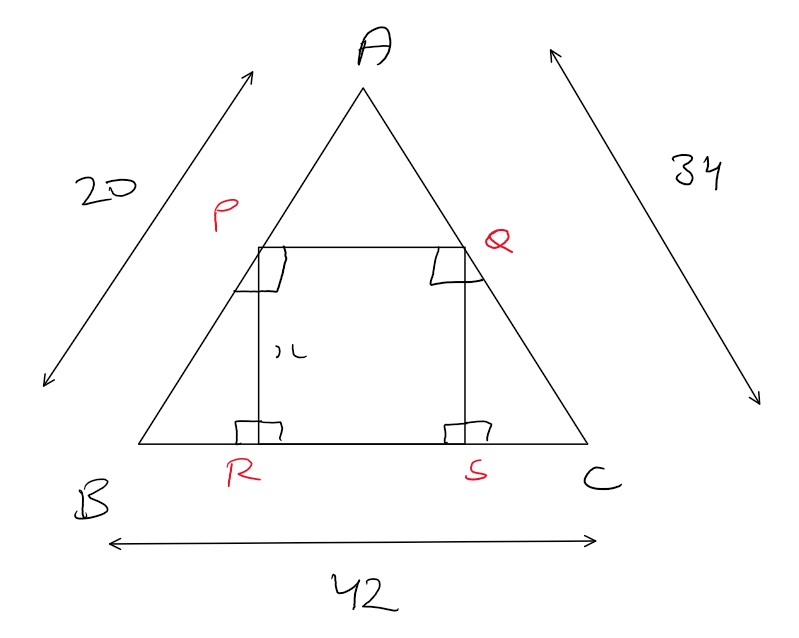
\includegraphics[width=0.5\linewidth]{Quant//Geometry//Images//Triangles/rodha_triangle_6_question_1.png}
\end{figure}

In a square, the sides are parallel to each other. We can use that property to make $\Triangle{APQ}$ similar to $\Triangle{ABC}$ as $\angle{APQ} = \angle{ABC} \text{and} \angle{AQP} = \angle{ACB}$ because they are corresponding angles respectively. Since these two angles are equal, $\Triangle{APQ}$ is similar to $\Triangle{ABC}$ through the AA similarity condition \\

To find the length of the square, we can draw a perpendicular AY intersecting PQ at point X. Since it is a perpendicular, the length of segment XY is equal to the side of square. \textbf{We can use the three sides of $\Triangle{ABC}$ to find $AY$ and compare ratio of sides with heights}

\begin{figure}[h!]
    \centering
    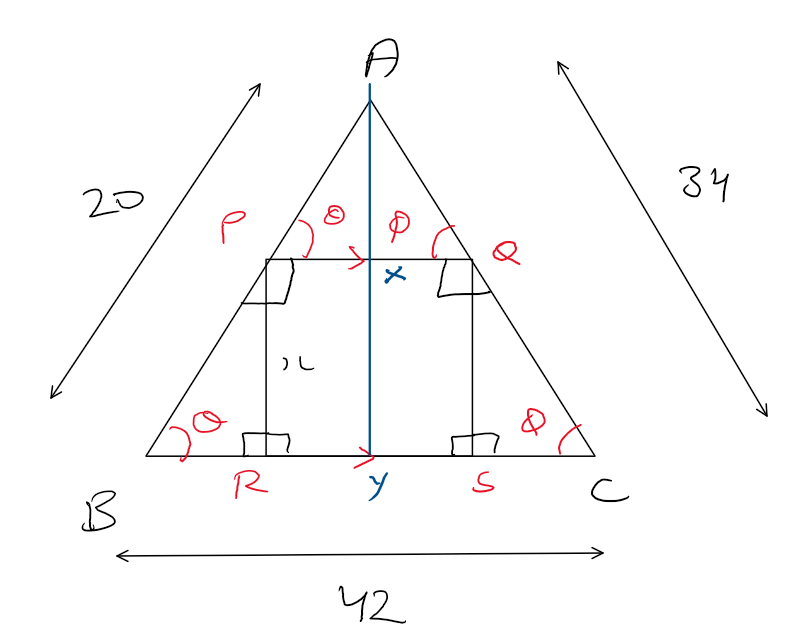
\includegraphics[width=0.5\linewidth]{Quant//Geometry//Images//Triangles/rodha_triangle_6_question_1_1.png}
\end{figure}

We can use the concept of pythagorean triplets to find the height $AY$. Let us take $\Triangle{AYC}$ where hypotenuse = $AC = 34$. Let us compare with a few common triplets. We can write $34 = 2 * 17$. \textit{While we can use any triplet to find a coefficient such that hypotenuse = 34 and triplet satisfies pythagorean theorem, for sake of easy calculation, let us keep to integer and simple values only}
\begin{itemize}
    \item 3,4,5 
    \item 5,12,13,
    \item 6,8,10
    \item 7,24,25
    \item 8,15,17 ... We can use this as it contains 17
\end{itemize}

We know that $34 = 2 * 17$. Therefore, for our triplet, our coefficient is 2 $\implies$ dimensions are 16,30 and 34. By observing our figure, we can say that $YC = 30$ and $AY = 16$. Now, let's use the similarity conditions between $\Triangle{APQ}$ and $\Triangle{ABC}$

\begin{align*}
    \dfrac{PQ}{BC} &= \dfrac{AX}{AY} \\
    \dfrac{x}{42} &= \dfrac{16 - x}{16} \tag{AX = AY - XY} \\
    16x &= 42 * 16 - 42x \\
    x &= \dfrac{42 * 16}{58} \\
    &= \dfrac{336}{29}
\end{align*}

\textbf{Note : Triangles 8 should be seen before Triangles 7}

\newpage


















\section{Conditions for Formation of Triangle}

\subsection{General Formula}
For a triangle, the relation of sides is as follows : Difference of two sides $<$ third side $<$ Sum of two sides. Refer to the following questions

\SampleQuestion{If sides of triangle are $(7,12,n)$, for how many integral values of $n$ the triangle will be formed?}

The third side $n$ is related to other sides $(7,12)$ as $12 - 7 < n < 12 + 7 \implies 5 < n < 19$. The number of values of $n$ is $19 - 5 - 1 = 13$

\SampleQuestion{If 2 sides of a triangle 762 and 1233 units. For how many integral values of 3rd side, a triangle will be formed}

The third side is related to other sides as : $1233 - 762 < \text{third side} < 1233 + 762 \implies 501 < \text{third side} < 1965$. The number of integral values is $1965 - 501 - 1 = 1523$

\subsection{Condition for right, obtuse and acute triangles}
We can use the pythagoreas theorem to deduce conditions through which we can determine whether a triangle is a right, obtuse or acute triangle. It is summarised in the below table for $\Triangle{ABC}$. The sides are marked as follows : $AC = c, BC = b, AB = a$. In the table below, \textbf{the side $c$ is assumed to be the largest}

\begin{table}[h!]
    \centering
    \begin{tabular}{|| c | c ||}
        \hline
         $\angle{ABC}$ & Condition  \\
        \hline
         $= \degree{90}$ & $c^2 = a^2 + b^2$ \\ 
        \hline
         $> \degree{90}$ & $c^2 > a^2 + b^2$ \\ 
        \hline
         $< \degree{90}$ & $c^2 < a^2 + b^2$ \\ 
        \hline
    \end{tabular}
\end{table}

To make sense of this, imagine a right triangle $ABC$ where $\angle{ABC} = \degree{90}$. If we increase the angle, we can see that the side $AC$ increases in response. Similarly, if we decrease the angle, the side decreases in response. This is because of a principle (more like an observation) : \textbf{Larger the angle, larger the side opposite to that angle}

\begin{figure}[h!]
    \centering
    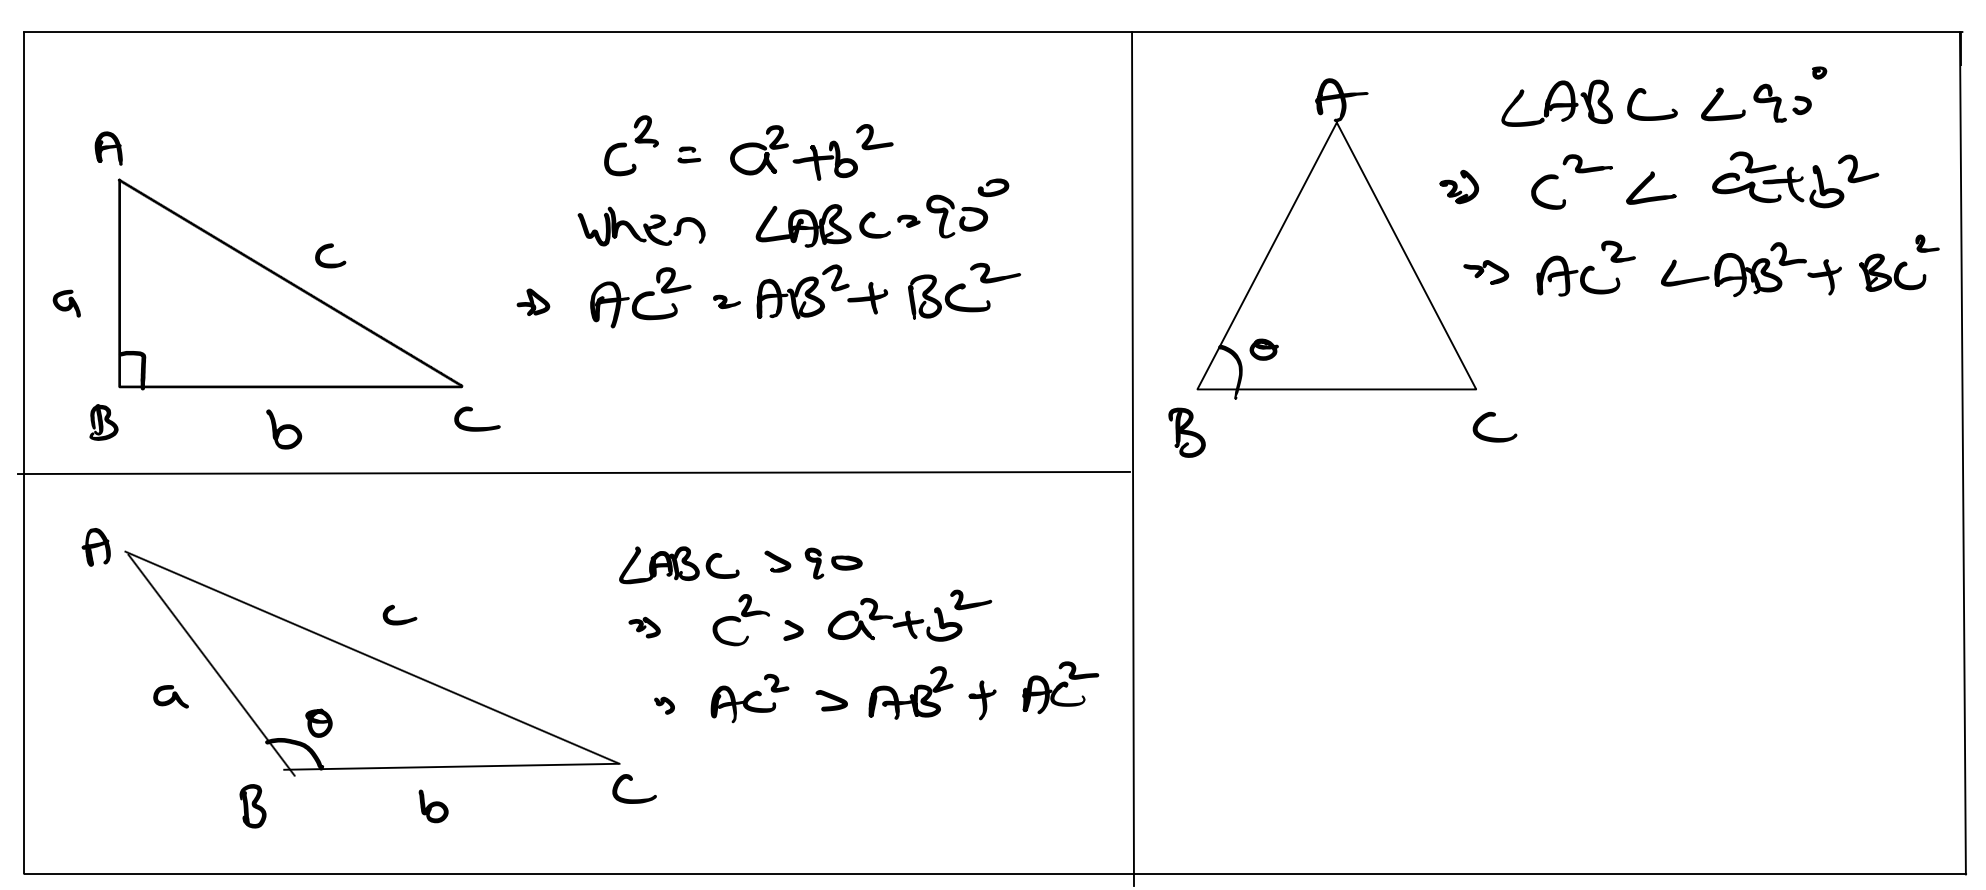
\includegraphics[width=1.0\linewidth]{Quant//Geometry//Images//Triangles/triangle_8_right_obtuse_acute_logic.png}
\end{figure}

\SampleQuestion{Determine whether a triangle with sides 12,18,23 is acute, obtuse or right}

Longest side = 23. Let use pythagoreas theorem to see how the longest side relates with other sides
\begin{align*}
    23^2 &= 12^2 + 18^2 \\
    529 &= 144 + 324 \\
    529 &> 468
\end{align*}

From above, we can conclude that the triangle is an obtuse triangle

\SampleQuestion{If 2 sides of a triangle are 8 and 15, then for how many integral values of 3rd side will the triangle will be an obtuse triangle?}

The range of values the third side can have is determined as $15 - 8 < n < 15 + 8 \implies 7 < n < 23$. We can have two scenarios

\begin{enumerate}
    \item The third side is the longest side
    \item 15 is the longest side
\end{enumerate}

In the cases below, let us assume that the third side is represented as $n$

\textbf{Case 1 : The third side is the longest side}
\begin{align*}
    n^2 &> 8^2 + 15^2 \\
    &> 64 + 225 \\
    &> 289 \\
    n &> \sqrt{289} = 17 \tag{$n$ in this case, will be a positive value only} 
\end{align*}

In this scenario, the values $n$ can take is 18,19,20,21,22

\textbf{Case 2 : 15 is the longest side}
\begin{align*}
    15^2 &> n^2 + 8^2 \\
    n^2 &< 225 - 64 \\
    n^2 &< 161 \\
    n &< \sqrt{161} \tag{$n$ in this case, will be a positive value only}
\end{align*}

In this case, the possible values $n$ can have is 8,9,10,11,12

Total values = 8,9,10,11,12,18,19,20,21,22


\newpage

















\section{Finding number of triangles when perimeter p is given}

\subsection{Nearest Integer Function (Round)}
For a decimal number $n$, the nearest integer function is represented as $\left [ n \right ]$. The behavior of this function can be seen as follows
\begin{itemize}
    \item $\Round{5.4} = 5$ : Acts as floor if value is less than 5.5
    \item $\Round{5.5} = 5$ : Acts as floor if value is equal to 5.5
    \item $\Round{5.6} = 6$ : Acts as ceil if value is greater than 5.5
\end{itemize}

\subsection{All Triangles}
\begin{equation*}
    \text{Number of triangles} = 
    \begin{cases}
        \Round{\dfrac{(p+3)^2}{48}} &\text{$p$ is odd} \\    \\
        \Round{\dfrac{p^2}{48}} &\text{$p$ is even}     
    \end{cases}
\end{equation*}

\subsection{Scalene Triangle}
In the above formula, substitute $p$ with $p-6$

\begin{equation*}
    \text{Number of triangles} = 
    \begin{cases}
        \Round{\dfrac{(p - 3)^2}{48}} &\text{$p$ is odd} \\    \\
        \Round{\dfrac{(p - 6)^2}{48}} &\text{$p$ is even}   
    \end{cases}
\end{equation*}

\subsection{Equilateral Triangle}
\begin{equation*}
    \text{Number of triangles} = 
    \begin{cases}
        0 &\text{If perimeter is not a multiple of 3}    \\
        1 &\text{If perimeter is not a multiple of 3}    \\
    \end{cases}
\end{equation*}

\subsection{Isoceles Triangle}
To get number of isoceles triangle, find count of all triangles and subtract number of scalene and isocelene triangles

\SampleQuestion{If $p = 16$, find the number of triangles that can be formed}

Since $p$ is even, the formula is $\Round{ \dfrac{p^2}{48} } \implies \Round{ \dfrac{16 * 16}{48} } = 5$

\SampleQuestion{If $p = 27$, find number of distinct triangles}
$p$ is odd therefore $\Round{ \dfrac{(p+3)^2}{48} } \implies \Round{ \dfrac{30 * 30}{48} } = 19$

\vspace{3cm}

\SampleQuestion{Find number of scalene triangles for the following values of $p$}
\begin{enumerate}
    \item 24
    \item 17
\end{enumerate}



$p = 24$ , Number of scalene triangles = $\Round{\dfrac{18 * 18}{48}} = 7$ \\

$p = 17$ , Number of scalene triangles = $\Round{\dfrac{14 * 14}{48}} = 4$

\SampleQuestion{Find number of isoceles triangle if $p=30$}

Number of isoceles triangles = all triangles - equilateral triangles - scalene triangles

\begin{itemize}
    \item All triangles : $\Round{\dfrac{30 * 30}{48}} = 19$
    \item Scalene triangles : $\Round{\dfrac{24 * 24}{48}} = 12$
    \item Equilateral triangles : 1 as 30 is divisible by 3
\end{itemize}

Isoceles triangle = $19 - 12 - 1 = 6$

\SampleQuestion{How many distinct triangles can be formed with integral sides if $p = 80$}
\begin{enumerate}
    \item With all sides even
    \item With 2 sides odd and 1 side even
\end{enumerate}

\textbf{With all sides even}
Let us assume that sides of triangle are $2a,2b,2c$. The perimeter is defined as
\begin{align*}
    2a + 2b + 2c &= 80 \\
    a + b + c &= 40
\end{align*}

Now, we can reduce the question to finding number of triangles where perimeter is 40. It is derived as $\Round{\dfrac{40 * 40}{48}} = 33$ \\

\textbf{2 sides odd and 1 side even}

\begin{WARNING}
    Let us assume that sides are $2a,2b+1,2c+1$. Perimeter is defined as $2(a+b+c+1) = 80 \implies a+b+c = 39$. Number of triangles are $\Round{\dfrac{42 * 42}{48}} = 37$ \\

    This is the wrong way of doing things. This is because for different values of $(a,b,c)$, the dimensions of triangle will be different. When we solve for the reduced triangle, then we also need to check if the values of a,b,c thus calculated also satisfy the triangle inequality for the original equation, i.e. for $2a-1, 2b-1, 2c$
\end{WARNING}

The correct way of solving this is to realise that if the perimeter of a triangle is even, it is due to following combinations only
\begin{itemize}
    \item All three even sides : $a + b + c$ where $a,b,c$ is even
    \item Two sides are odd and one is even : $a + b +c$ where $a$ is even and $b,c$ are odd
    \item We cannot have all three odd as their sum will be odd
\end{itemize}

Since we already computed values for the case where all sides are even in the above part (33), we can now find for "one odd and two even" as $all - even$ \\

Finding count of all triangles : $\Round{\dfrac{80 * 80}{48}} = 133$. "one even and two odd" is $133 - 33 = 100$

\SampleQuestion{How many distinct triangles can be formed with integral sides if perimeter is 39 with the following conditions}
\begin{enumerate}
    \item With all sides odd
    \item With 2 sides even and 1 side odd
\end{enumerate}

Let us make an observation that we made in above question. If a triangle has an odd perimeter, it can be achieved with the following combinations only
\begin{itemize}
    \item 3 odd sides
    \item 2 even sides and 1 odd side
    \item We cannot have 2 odd sides and 1 side because sum of odd sides will be even
\end{itemize}

\textbf{All sides odd}

Let sides be 2a-1, 2b-1, 2c-1. Perimeter is therefore
\begin{align*}
    2 (a + b + c) - 3 &= 39 \\
    a + b  + c &= 21
\end{align*}

For this reduce triangle, the number of triangles are $\Round{\dfrac{24 * 24}{48}} = 12$

\textbf{2 Even sides and 1 odd side}

To calculate this, we find difference of all triangles and all odd side triangles. All triangles : $\Round{\dfrac{42 * 42}{48}} = 37$. 

Answer = 37 - 12 = 25

\SampleQuestion{If perimeter of a triangle is 60, then which of the following cannot be the area of a triangle?}
\begin{enumerate}
    \item 151
    \item 159
    \item 169
    \item 176
\end{enumerate}

\textbf{For a constant perimeter $p$, maximum area of a triangle is of an equilateral triangle}. Area of equilateral triangle : $\dfrac{\sqrt{3} * a^2}{4}$ where $a$ is the side of triangle. In this case, $a = 20$. 

\begin{align*}
    \text{Area} &= \dfrac{\sqrt{3} * 20 * 20}{4} \\
    &=  100 * 1.732 \\
    &= 173.2
\end{align*}

Since the max area of the triangle can be 173.2, the option 176 can be eliminated

\newpage


















\section{Sine and Cosine Rule}
Sine and Cosine rule are relations between angles and sides of a triangle. They are explained as follows
\begin{itemize}
    \item Sine rule says that the ratio of angle and side opposite to it is equal.
    \item Cosine rule relates an angle and the three sides of a triangle 
\end{itemize}

\begin{figure}[h!]
    \centering
    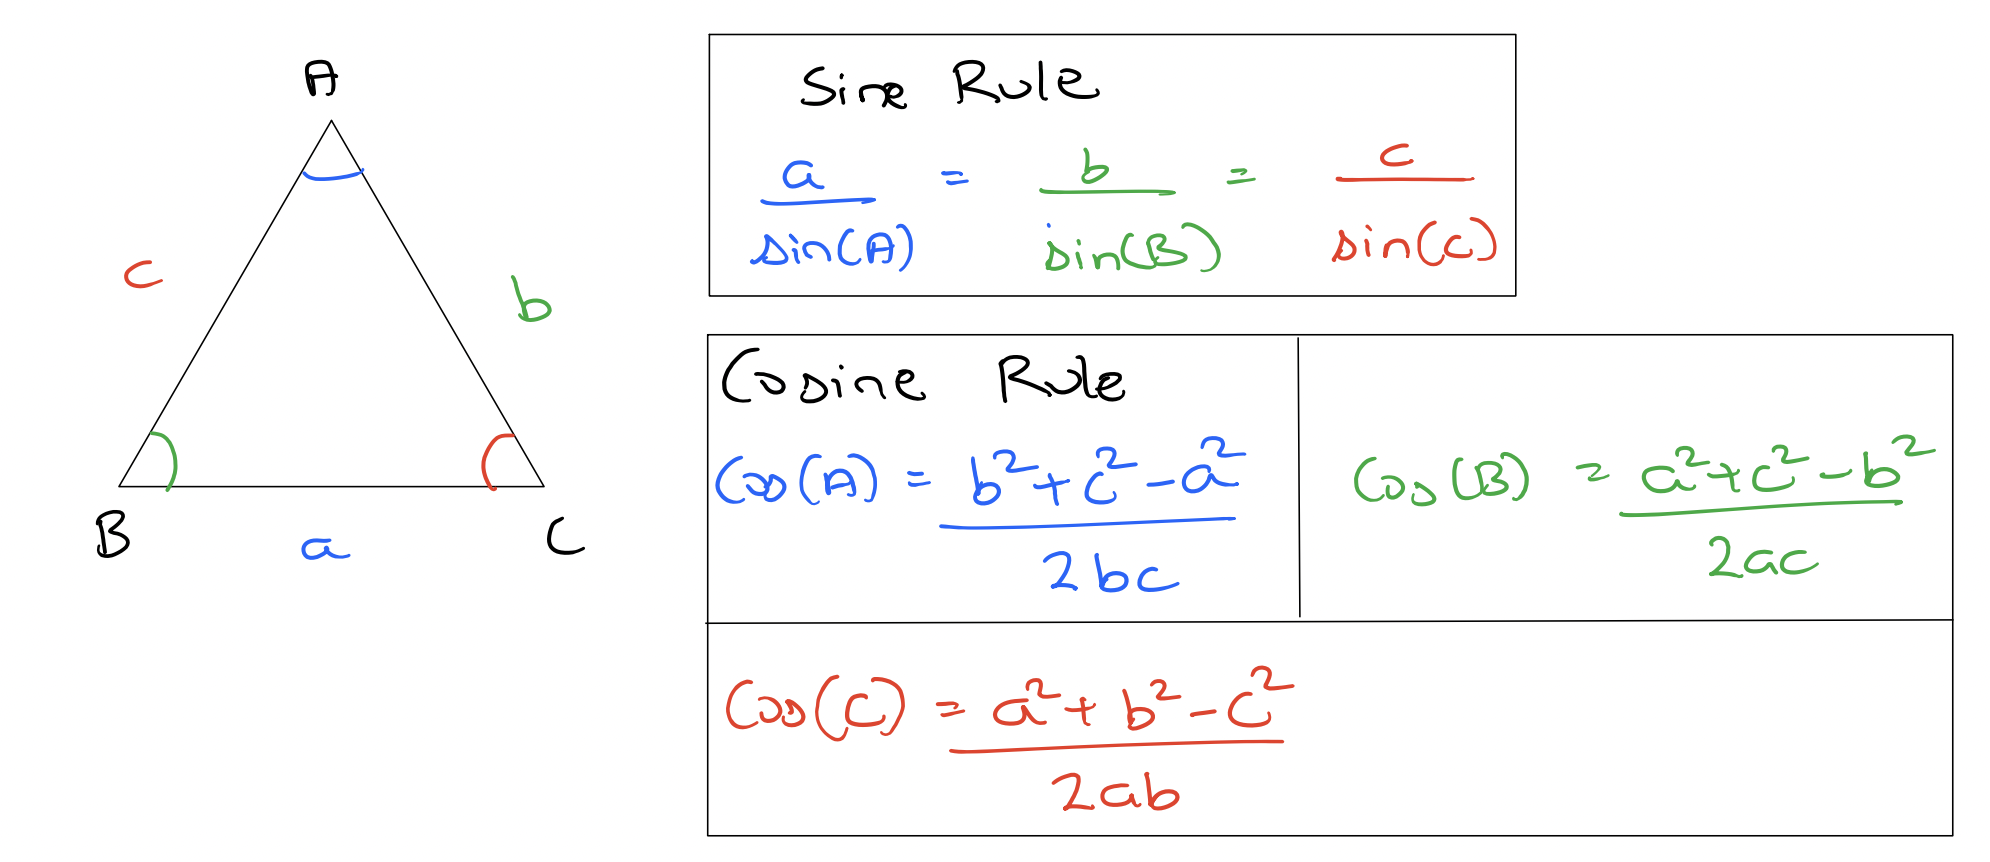
\includegraphics[width=1\linewidth]{Quant//Geometry//Images//Triangles/triangles_10_sine_and_cosine_rule.png}
\end{figure}

To apply this rule correctly, we need to understand the opposite sides and other sides. For the above $\Triangle{ABC}$, refer to the following table

\begin{table}[h!]
    \centering
    \begin{tabular}{|| c | c | c ||}
        \hline
         Angle & Opposite Side & Other Sides  \\
        \hline
         $\angle{A}$ & BC (a) & AC (b) , AB(c) \\ 
        \hline
         $\angle{B}$ & AC (b) & BC (a) , AB(c) \\ 
        \hline
         $\angle{C}$ & AB (c) & BC (a) , AC(b) \\ 
        \hline
    \end{tabular}
\end{table}

Using this, we can write sine and cosine rules as
\begin{itemize}
    \item Sine rule = $\dfrac{\text{opposite side}}{\text{angle}}$

    \item Cosine rule = $\dfrac{\text{sum of square of other sides - opposite side}}{2 * \text{product of other sides}}$
\end{itemize}

\newpage

\SampleQuestion{PM is angle bisector of $\Triangle{PQR}$ on base $QR$ and $\angle{Q} + \angle{R} = \degree{120}$. Find the length of $QR$ and $PM$}

\begin{figure}[h!]
    \centering
    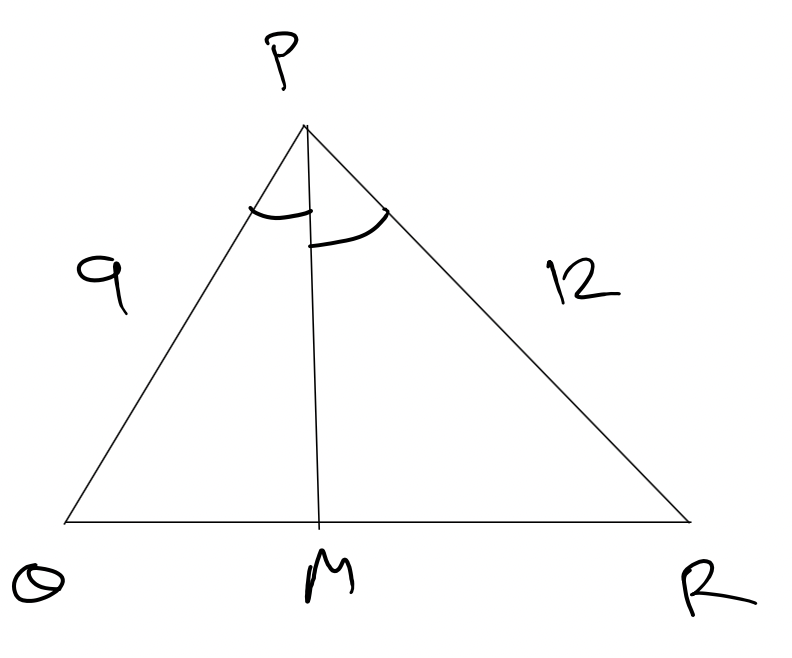
\includegraphics[width=0.35\linewidth]{./Quant/Geometry/Images/Triangles/triangle_10_question_1_img.png}
\end{figure}

\textbf{Finding QR}

To find QR, let's first find the value of $\angle{P}$ and then apply cosine rule. According to the question, $\angle{Q} + \angle{R} = \degree{120}$. This means that $\angle{P} = \degree{60}$

Applying cosine rule on $\angle{P}$
\begin{align*}
    \cos{P} &= \dfrac{12^2 + 9^2 - QR^2}{2 * 12 * 9} \\
    \cos{60} &= \dfrac{144 + 81 - QR^2}{24 * 9} \\
    \dfrac{24 * 9}{2} &= 225 - QR^2 \\
    QR &= \sqrt{225 - 108} \\
    QR &= \sqrt{117} \\
    QR &= 3 \sqrt{13}
\end{align*}

\textbf{Finding PM}
\begin{WARNING}
    PM is not perpendicular
\end{WARNING}

We can find area of PQR by adding areas of PQM and PRM. Using trigonometric formulae, we can find areas as follows
\begin{align*}
    \dfrac{PQ * PR * \sin{\angle{QPR}}}{2} &= \dfrac{PQ * PM * \sin{\angle{QPM}}}{2} + \dfrac{PM * PR * \sin{\angle{RPM}}}{2} \\
    9 * 12 * \dfrac{\sqrt{3}}{2} &= PM * (9 \sin{30} + 12 \sin{30}) \\
    54 \sqrt{3} &= \dfrac{PM}{2} * 21 \\
    PM &= \dfrac{54 * 2 * \sqrt{3}}{21} \\
    PM &= \dfrac{36 \sqrt{3}}{7}
\end{align*}

% \SampleQuestion{One of the sides of an obtuse angled isosceles triangle of perimeter 180cm is 80cm. What is the distance between incentre and circumcentre of this triangle?}

\SampleQuestion{An isoceles triangle with $\angle{P} = \degree{120}$ has an area of $16 \sqrt{3}$. What is its perimeter?}

\begin{figure}[h!]
    \centering
    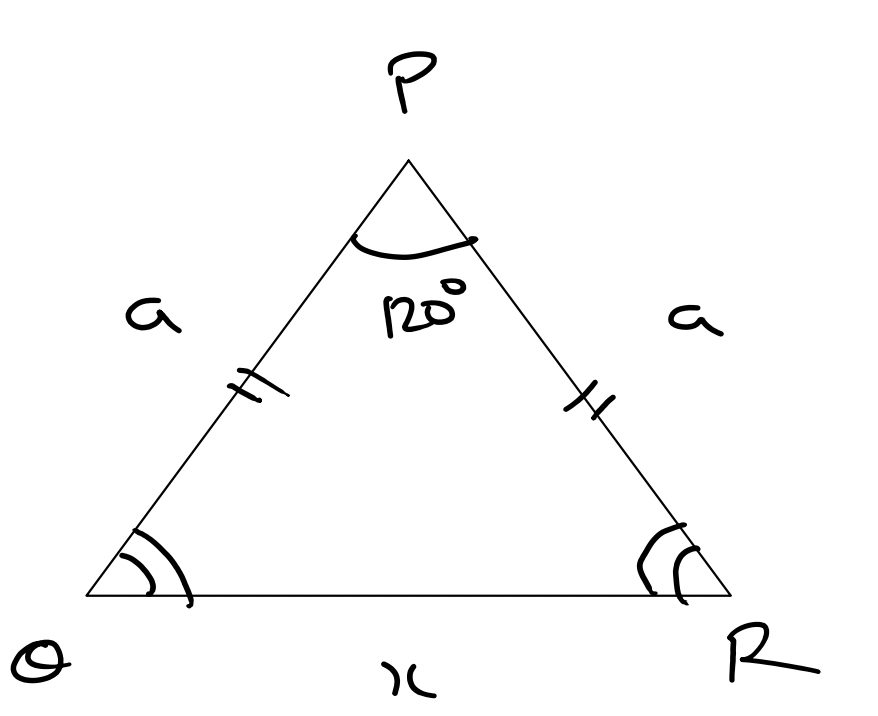
\includegraphics[width=0.5\linewidth]{Quant//Geometry//Images//Triangles/triangles_11_question_1.png}
\end{figure}

Since $\Triangle{PQR}$ is an isocles triangle, two of its sides will be equal. There is a property of isoceles triangle that if two sides are equal, then angles of those sides are equal as well. Therefore, in the above figure
\begin{itemize}
    \item PQ = PR $a$
    \item $\angle{PQR} = \angle{PRQ}$
\end{itemize}

We can understand that the value of $\angle{PQR} = \angle{PRQ} = \degree{30}$ because of the angle sum property of triangle (sum of all angles = $\degree{180}$. We now need to find the value of $a$ using area of triangle. Since we have two sides and the angle between them, we can use the trigonometric formula

\begin{align*}
    16 \sqrt{3} &= \dfrac{1}{2} * a^2 * \sin{120} \\
    32 \sqrt{3} &= a^2 * \dfrac{\sqrt{3}}{2} \tag{$\sin{(180 - x)} = \sin{x}$} \\
    a &= 8
\end{align*}

We can use sine rule to find the value of $x$ dimension. For below, we will use $\angle{PQR}$ and $\angle{QPR}$

\begin{align*}
    \dfrac{a}{\sin{30}} &= \dfrac{c}{\sin{120}} \\
    2a &= \dfrac{2}{\sqrt{3}} c \\
    c &= 8 \sqrt{3}
\end{align*}

Perimeter = $8 + 8 + 8\sqrt{3} \implies 16 + 8\sqrt{3}$

\newpage










\section{Area of triangle by ratio of sides}

\subsection{Using common height}

If two triangles share a common height and a line segment divides the base in a ration $x:y$, then we can say that the areas are divided in the ratio $x:y$ as well. In the below figure, we have $\Triangle{ABC}$ where $AD$ divides $BC$ in ratio $3:2$. $AP$ is a perpendicular. According to this, $BD = 3x, DC = 2x \implies BC = 5x$

\begin{figure}[h!]
    \centering
    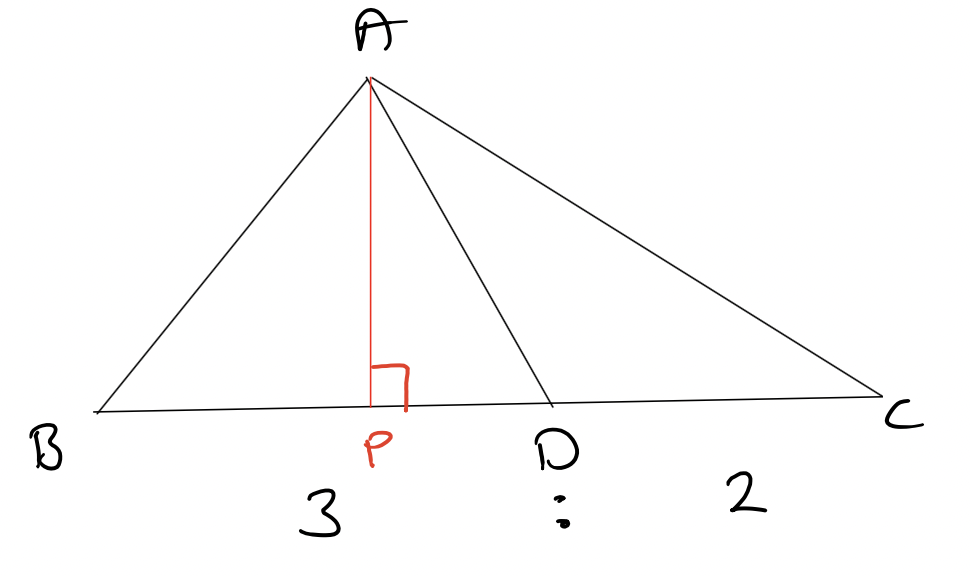
\includegraphics[width=0.4\linewidth]{Quant//Geometry//Images//Triangles/triangles_11_common_height_area.png}
\end{figure}

\begin{itemize}
    \item Area of $\Triangle{ABD}$ : The $\Triangle{ABD}$ has base $BD$ and height $AP$. The area is defined as $\frac{1}{2} * BD * AP$
    \item Area of $\Triangle{ACD}$ : The $\Triangle{ACD}$ has base $CD$ and height $AP$. The height remains same anyway, even if the height is "outside" the triangle. The area is defined as $\frac{1}{2} * CD * AP$
    \item Area of $\Triangle{ABC}$ : The $\Triangle{ABC}$ has base $BC$ and height $AP$. The area is defined as $\frac{1}{2} * BC * AP$. Since $BC = 5x$, Let us denote area of $\Triangle{ABC}$ as $5A$ where $A = \frac{1}{2} * x * AP$
    \item For area of $\Triangle{ABD}$, we can write it as $\frac{1}{2} * 3x * x * AP = 3A$
    \item For area of $\Triangle{ACD}$, we can write it as $\frac{1}{2} * 2x * x * AP = 2A$
\end{itemize}

Thus, we can see that the divided triangles have their area divided in the same ratio as well
\begin{itemize}
    \item Area$(\Triangle{ABD}) =$ $\dfrac{3}{5} \text{ Area }(\Triangle{ABC})$
    \item Area$(\Triangle{ACD}) =$ $\dfrac{2}{5} \text{ Area }(\Triangle{ABC})$
\end{itemize}

Following the above logic, we can quickly derive relationships of triangles based on their area. In the below triangle, where $BD$ divides $AC$ in ratio $2:3$

\begin{figure}[h!]
    \centering
    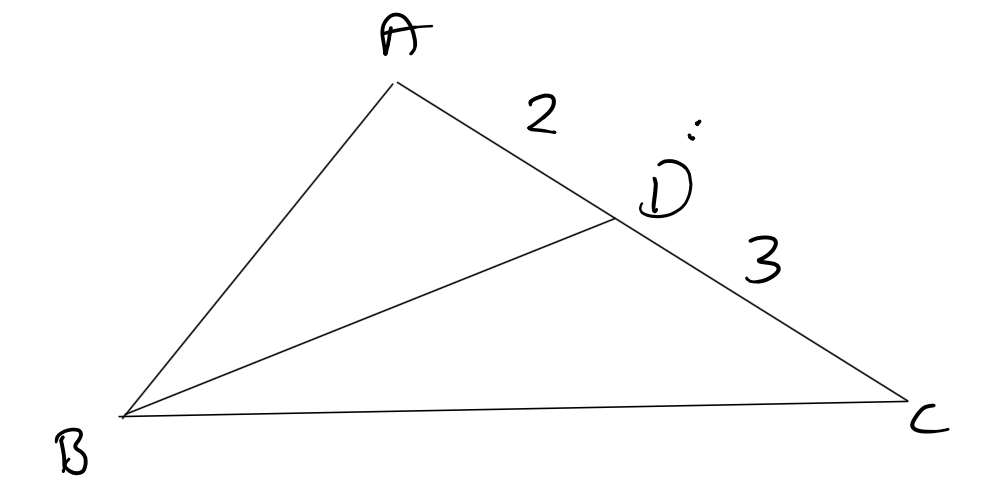
\includegraphics[width=0.4\linewidth]{Quant//Geometry//Images//Triangles/triangle_11_common_height_1.png}
\end{figure}

\begin{itemize}
    \item $\Area{\Triangle{ABD}} = \dfrac{2}{5} \Area{\Triangle{ABC}}$
    \item $\Area{\Triangle{BDC}} = \dfrac{3}{5} \Area{\Triangle{ABC}}$
\end{itemize}

\vspace{2cm}

\subsection{Using common angle}
We can also use the common angle between two triangles to find ratio of area of those triangles

\begin{figure}[h!]
    \centering
    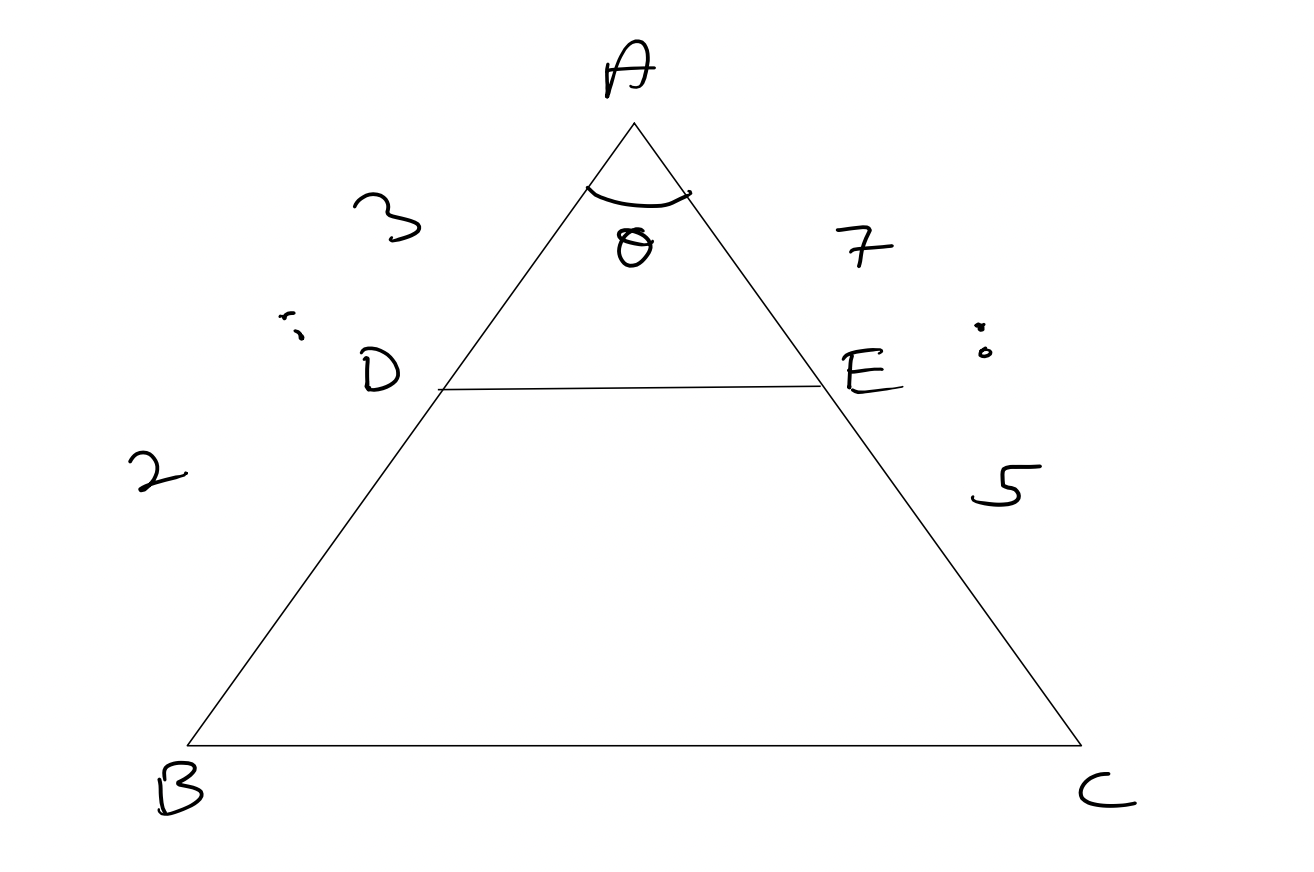
\includegraphics[width=0.5\linewidth]{./Quant/Geometry/Images/Triangles/triangle_11_common_angle_area.png}
\end{figure}

The common angle in this case is $\theta$ or $\angle{BAC}$. We can see from the figure that $AB = 5x$ and $AC = 12y$. We can find the respective areas using the formula $\dfrac{1}{2} ab \sin{\theta}$

\begin{itemize}
    \item $\Area{\Triangle{ABC}} = \dfrac{1}{2} * 5x * 12y$
    \item $\Area{\Triangle{ADE}} = \dfrac{1}{2} * 3x * 7y$
\end{itemize}

The ratio $\Area{\Triangle{ADE}}:\Area{\Triangle{ABC}} $ is
\begin{align*}
    \dfrac{\Area{\Triangle{ADE}}}{\Area{\Triangle{ABC}}} &= \dfrac{3 * 7}{5 * 12} \\
    \Area{\Triangle{ADE}} &= \dfrac{3}{5} * \dfrac{5}{12} \Area{\Triangle{ABC}} \\
    &= \dfrac{AD}{AB} * \dfrac{AE}{AC} * \Area{\Triangle{ABC}} \\
\end{align*}

\SampleQuestion{$DE$ divides $AC$ in ratio $8:5$ and $AB$ in ratio $4:3$. Find ratio of area of $ADE$ and $BDEC$}

\begin{figure}[h!]
    \centering
    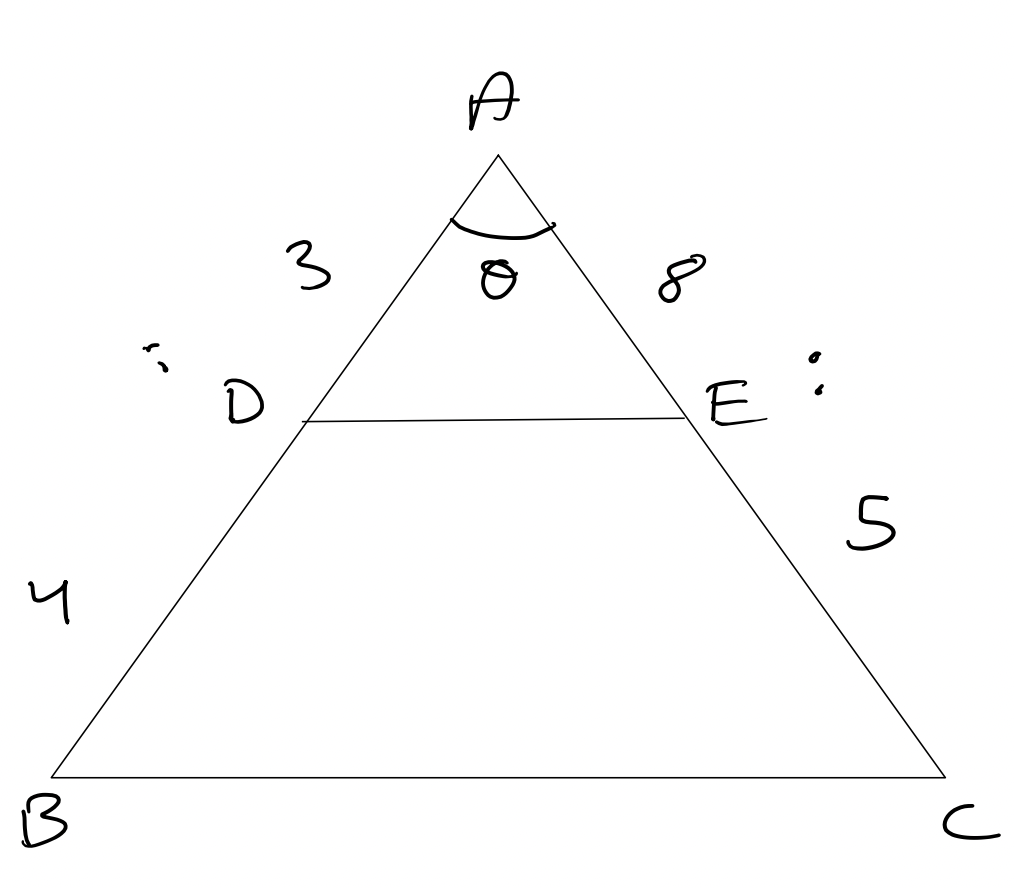
\includegraphics[width=0.3\linewidth]{Quant//Geometry//Images//Triangles/triangle_11_question_1_area.png}
\end{figure}

From our discussions above, we know that $\Area{\Triangle{ADE}} = \dfrac{3}{7} * \dfrac{8}{13} \Area{\Triangle{ABC}} \implies \dfrac{24}{91} \Area{\Triangle{ABC}}$. Using this, we can find area of quadilateral in terms of $\Triangle{ABC}$

\begin{align*}
    \Area{BDEC} &= \Area{ABC} - \dfrac{24}{91} \Area{ABC} \\
    &= \dfrac{67}{35} \Area{ABC}
\end{align*}

Ratio is therefore, $\dfrac{24 * 91}{67 * 91} = 24:67$



\SampleQuestion{DE divides AB in 5:4 and AC in 2:3. EF divides BC in 3:5. Find ratio of area of DEF and ABC}

\begin{figure}[h!]
    \centering
    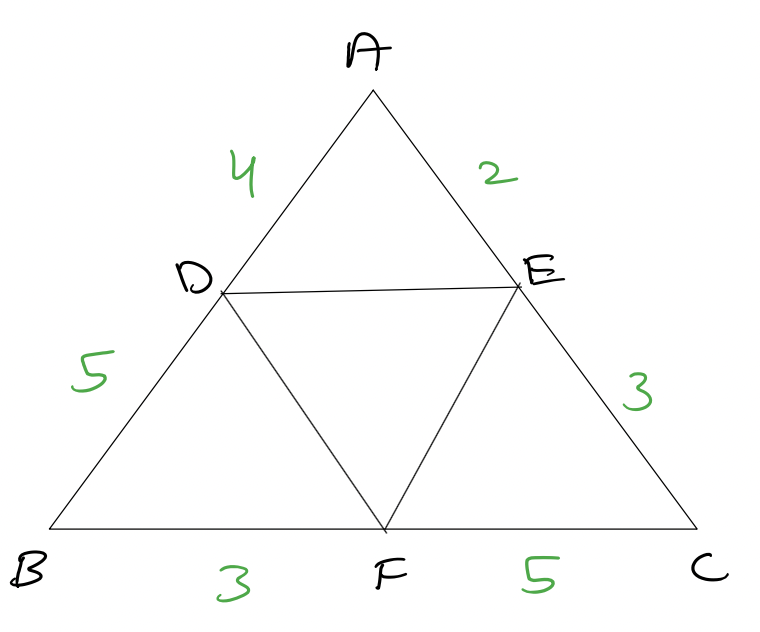
\includegraphics[width=0.5\linewidth]{Quant//Geometry//Images//Triangles/triangle_11_question_2_area.png}
\end{figure}

This is an interesting question. $\Area{DEF} = \Area{ABC} - (\Area{ADE} + \Area{BDF} + \Area{EFC})$. Using ratios, we can find $\Area{ADE},\Area{BDF},\Area{EFC}$ in terms of $\Area{ABC}$

\begin{itemize}
    \item $\Area{ADE} = \dfrac{4}{9} * \dfrac{2}{5} \Area{ABC} \impliedby \dfrac{8}{45} \Area{ABC}$
    
    \item $\Area{BDF} = \dfrac{5}{9} * \dfrac{3}{8} \Area{ABC} \impliedby \dfrac{15}{72} \Area{ABC} \implies \dfrac{5}{24} \Area{ABC}$
    
    \item $\Area{EFC} = \dfrac{3}{5} * \dfrac{5}{8} \Area{ABC} \impliedby \dfrac{3}{8} \Area{ABC}$

    \item $(\Area{ADE} + \Area{BDF} + \Area{EFC}) = \Area{ABC} * (\dfrac{8}{45} + \dfrac{5}{24} + \dfrac{3}{8}) \implies \dfrac{137}{180} \Area{ABC}$

    \item $\Area{DEF} = \Area{ABC} ( 1 - \dfrac{137}{180} ) \implies \dfrac{43}{180} \Area{ABC} \implies \Area{DEF} : \Area{ABC} = 43:180$

\end{itemize}

\newpage




\section{Midpoint Theorem and Proportionality Theorem}

\subsection{Midpoint Theorem}
In a triangle, if from the midpoint of a triangle, a parallel line is drawn to other side of the triangle such that it is parallel with a side of triangle, the endpoint of the newly drawn line will be a midpoint to the other side and the length of this parallel line will be half of the side it is parallel with \\

In below figure, D is a midpoint of AB. We have drawn DE, which is parallel to BC. The vertex E acts as the midpoint of line AC

\begin{figure}[h!]
    \centering
    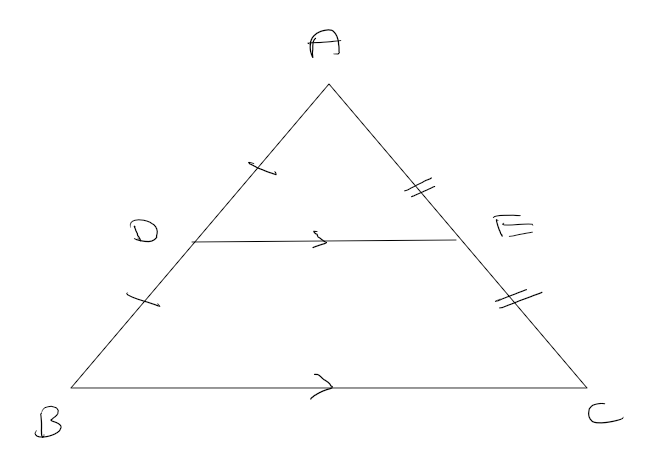
\includegraphics[width=0.5\linewidth]{Quant//Geometry//Images//Triangles/triangle_12_midpoint_theorem_result.png}
\end{figure}

The basis of this property is similarity of triangles. In the above figure, we can easily prove that $\Triangle{ADE}$ is similar to $\Triangle{ABC}$ by AA similarity condition. In similar triangles, ratio of sides is equal. If D is the midpoint of AB then $\dfrac{AD}{AB} = \dfrac{1}{2}$. Using the rules of similarity, $\dfrac{AD}{AB} = \dfrac{DE}{BC} = \dfrac{AE}{AC} = \dfrac{1}{2}$. Thus
\begin{itemize}
    \item E is midpoint of AC as $\dfrac{AE}{AC} = \dfrac{1}{2}$
    \item $DE = \dfrac{1}{2} BC$ as $\dfrac{DE}{BC} = \dfrac{1}{2}$
\end{itemize}

\SampleQuestion{In the figure below, BC = 16 and AM = 12. N is midpoint of AC and T is midpoint of BM. AM is perpendicular to BC. Find the length of TN}

\begin{figure}[h!]
    \centering
    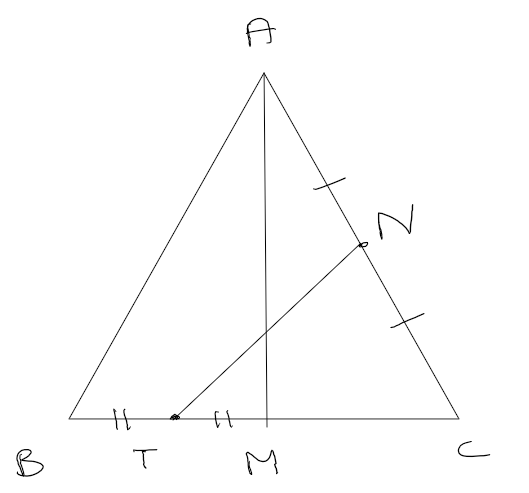
\includegraphics[width=0.35\linewidth]{Quant//Geometry//Images//Triangles/triangle_12_midpt_question_1.png}
\end{figure}

A general rule to remember is that whenever we have to find the length of a line that is not either perfectly vertical or horizontal, we can use pythagoreas theorem. We can split any "angled" line into a horizontal and vertical component, find those lengths and then use pythagoreas theorem to find the actual length. In the triangle, we can create a line NR parallel to AM on BC. 

\begin{figure}[h!]
    \centering
    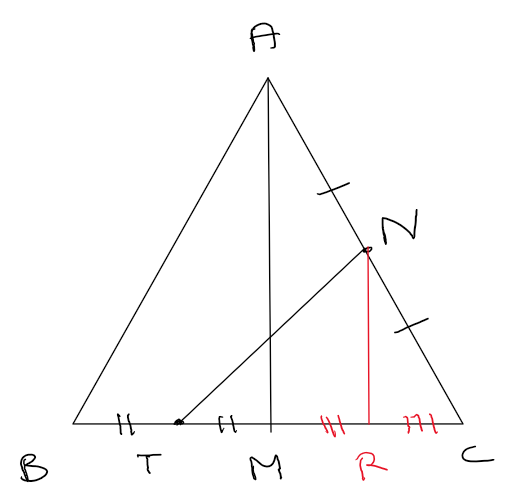
\includegraphics[width=0.35\linewidth]{Quant//Geometry//Images//Triangles/triangle_12_midpoint_q1_ans_1.png}
\end{figure}

Since NR is parallel to AM (and also perpendicular. Any line that is parallel to a perpendicular is a perpendicular itself), we can apply midpoint theorem and say that R is the midpoint of MC. Also, NR = $\dfrac{AM}{2} \implies \dfrac{12}{2} = 6$ because of midpoint theorem as well. \\

To calculate TN, we now need TR as well so that we can apply pythagoreas theorem. We can see that 
\begin{align*}
    BC &= BM + MC \\
    16 &= BT + TM + MR + CR \\
    16 &= 2 (TM + MR) \tag{BT = TM and MR = CR} \\
    TM + MR &= 8 \\
    TR &= 8 \tag{TM + MR = TR}
\end{align*}

Now, we can apply pythagoreas theorem in $\Triangle{NTR}$ and we will get $TN = 10$

\newpage
\SampleQuestion{In the below figure, P is the midpoint of AN and N is the midpoint of BC. Answer the following}
\begin{itemize}
    \item Find $AQ : QC$
    \item If $\Area{\Triangle{ABC}} = 120$, find $\Area{\Triangle{APQ}}$
\end{itemize}

\begin{figure}[h!]
    \centering
    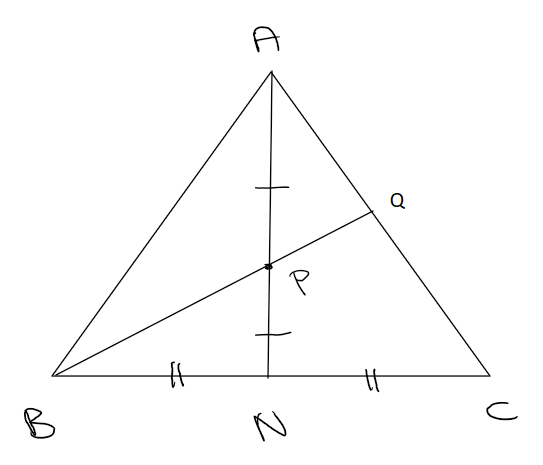
\includegraphics[width=0.35\linewidth]{Quant//Geometry//Images//Triangles/triangle_12_midpt_q2_img.png}
\end{figure}

We need to find someway through which we can get a relation between AQ and QC. Since N and P are midpoints, we can use midpoint theorem to simplify our work. In $\Triangle{BQC}$, we can apply midpoint theorem by constructing a line NR which is parallel to BQ. Because of this, QC will be split into two equal parts QR and CR

\begin{figure}[h!]
    \centering
    \includegraphics[width=0.35\linewidth]{Quant//Geometry//Images//Triangles/triangle_12_midpt_q2_ans_image_1.png}
\end{figure}

We can also determine that if NR is parallel to BQ, then it must be parallel to PQ as well as PQ is a part of BQ. Therefore, in $\Triangle{ANR}$, according to midpoint theorem, Q is midpoint of AR meaning AQ = AR. 
\begin{align*}
    AC &= AQ + QR + CR \\
    &= 3 AQ \tag{AQ = QR and QR = RC as proved above} \\
    AQ &= \dfrac{1}{3} AC
\end{align*}

From above, we can see that $QC = \dfrac{AC}{2}$ and thus, $AQ : QC = 1 : 2$ \\

If area of $\Triangle{ABC}$ is 120, then we can say that $\Area{ANC} = 60$ as N is midpoint of BC. We can zoom in on $\Triangle{ANC}$ and observe that Q divides AC into two sides of ratio $1 : 2$ (AQ : QC). Similarly, P divides AN in two equal parts. According to what we discussed about triangles having common height and ratio of sides, $\Area{\Triangle{APQ}} = \dfrac{1}{2} * \dfrac{1}{3} * \Area{\Triangle{ANC}} \implies \dfrac{60}{6} = 10$

\newpage

\subsection{Proportionality Theorem}

If 2 parallel lines are intersected at different points by transversals from the same point, then the ratio of those segments are equal.

\begin{figure}[h!]
    \centering
    \includegraphics[width=0.6\linewidth]{Quant//Geometry//Images//Triangles/triangle_12_proportionality_theorem_img.png}
\end{figure}

In the above figure, $PQ || XY$ (PQ is parallel to XY) and we have three transversals AC, AH and AS all originating from same point A. According to the theorem, $\dfrac{AB}{BC} = \dfrac{AG}{GH} = \dfrac{AR}{RS}$

\SampleQuestion{In the below figure, AE = 14, ED = 10, DC = 12, CA = 16, $AB : BC = 3 : 5$. Find the area of the shaded region $\Triangle{EFD}$}
\begin{figure}[h!]
    \centering
    \includegraphics[width=0.5\linewidth]{Quant//Geometry//Images//Triangles/triangle_12_midpt_propo_q1.png}
\end{figure}

This is an interesting question. We can find the dimension AD using concept of pythagorean triplets (or simply applying pythagoreas theorem). The triplet in $\Triangle{ACD}$ resembles (3,4,5) with a multiplier of 4 $\implies$ (12,16,20). Therefore, AD = 20 \\

Since DC and EB are parallel, we can see that a vertex A has two transversals AC and AD intersecting these lines. According to proportionality theorem, $\dfrac{AB}{BC} = \dfrac{AF}{FD} = \dfrac{3}{5}$. In $\Triangle{AED}$, the line EF divides AD in ratio $3 : 5$. Therefore, $\Area{\Triangle{EFD}} = \dfrac{5}{8} * \Area{\Triangle{AED}}$ \\

Using heron's formula, we will calculate $\Area{\Triangle{AED}}$
\begin{align*}
    s &= \dfrac{14 + 10 + 20}{2} = 22 \\
    \Area{\Triangle{AED}} &= \sqrt{22 * (22 - 20) * (22 - 10) * (22 - 14)} \\
    &= \sqrt{(2 * 11) * (2) * (2 * 2 * 3) * (2 * 2 * 2)} \\
    &= \sqrt{2^7 * 3 * 11} \\
    &= 8 \sqrt{66}
\end{align*}

$\Area{\Triangle{FED}} = \dfrac{8 * 5 \sqrt{66}}{8} = 5 \sqrt{66}$

\newpage











\section{Equilateral Triangles}
In an equilateral triangle, we have the following properties
\begin{itemize}
    \item All sides are equal (represented as $a$ in below figure)
    \item All angles are $\degree{60}$
    \item Centroid , Orthocenter , Incenter and Circumcenter are at the same point
    \item Median is perpendicular to the base $\implies$ median is a perpendicular bisector
\end{itemize}

\begin{figure}[h!]
    \centering
    \includegraphics[width=0.5\linewidth]{Quant//Geometry//Images//Triangles/triangle_13_equilateral_theory.png}
\end{figure}

Using the above figure, we can derive some results
\begin{itemize}
    \item Height
    \begin{itemize}
        \item D is a midpoint of BC $\implies BD = \dfrac{a}{2}$
        \item Taking BD as base in $\Triangle{ABD}$, we can find height AD as $\dfrac{AD}{BD} = \tan{\degree{60}} \implies AD = \dfrac{\sqrt{3} a}{2}$
    \end{itemize}

    \item Area : Using $\dfrac{1}{2} * \text{ base } * \text{ height }$ formula, we get $\dfrac{1}{2} * a * \dfrac{a \sqrt{3}}{2} = \dfrac{\sqrt{3} a^2}{4}$

    \item Inradius and Circumradius
    \begin{itemize}
        \item AD is a median and O is a centroid. Therefore, $AO : OD = 2 : 1$. Now, $OD$ is inradius and $OA$ is circumradius $\implies \dfrac{R}{r} = 2$
        \item Relating with height, we get $r = \dfrac{1}{3} * \dfrac{\sqrt{3} a}{2} \implies \dfrac{a}{2 \sqrt{3}}$
        \item Relating with height, we get $R = \dfrac{2}{3} * \dfrac{\sqrt{3} a}{2} \implies \dfrac{a}{\sqrt{3}}$
    \end{itemize}
\end{itemize}
\newpage

\SampleQuestion{There is an equilateral triangle with side of 2 units. A circle is inscribing it and another circle is circumscribing it. The circle circumscribing it is inscribed inside another equilateral triangle as shown in the figure below. Find the area of the bigger equilateral triangle}

\begin{figure}[h!]
    \centering
    \includegraphics[width=0.5\linewidth]{Quant//Geometry//Images//Triangles/triangle_13_q1.png}
\end{figure}

We can use the above results to easily calculate this. For the inner triangle, all measurements will have a subscript of $i$ and for outer triangle, a subscript of $o$. For example, side of inner triangle is $a_i$ and outer triangle is $a_o$

\begin{itemize}
    \item $R_i = \dfrac{a_i}{\sqrt{3}}$
    \item The circumradius of inner triangle is the inradius of the bigger triangle $\implies r_o = R_i$
\end{itemize}

\begin{align*}
    r_o &= \dfrac{a_o}{2 \sqrt{3}} \\ 
    \dfrac{a_i}{\sqrt{3}} &= \dfrac{a_o}{2 \sqrt{3}} \\
    a_o &= 2 a_i \\
    a_o &= 4 \tag{$a_i = 4$ is given}
\end{align*}

Area of outer triangle : $\dfrac{\sqrt{3} * 16}{4} = 4 \sqrt{3}$


%--------------------------------------------------------------------
%--------------------------------------------------------------------
%--------------------------------------------------------------------

% \part{Arithmetic}

% \chapter{Speed math}
% \section{Multiplying two numbers}
The idea is to split the number to nearest tens and simplify multiplication. See the following examples

\SampleQuestion{Find 153.27 * 15}
\begin{align*}
    153.27 * 15 &= (100 + 53.27) * 15 \\
    &= 1500 + (50 + 3.27) * 15 \\
    &= 1500 + 750 + (3 + 0.27) * 15 \\
    &= 2250 + 45 + (10 + 5) * 0.27 \\
    &= 2295 + 2.7 + 1.35 \\
    &= 2297.7 + 1.35 \\
    &= 2299.05
\end{align*}

\section{Approximating Percentages}
If we want to approximate percentages, we can use the following values and get closer to the required value 

\begin{table}[h!]
    \centering
    \begin{tabular}{|| c | c ||}
        \hline
         \textbf{Percentage} & \textbf{Divide}\\
        \hline
         10\% & Number by 10 \\
        \hline
         5\% & 10\% of number by 2 \\
        \hline
         1\% & Number by 100 \\
        \hline
         25\% & Number by 4 \\
        \hline
         50\% & Number by 2 \\
        \hline
    \end{tabular}
\end{table}

Other values can be derived using addition, subtraction and multiplication of above values. Let us do some examples. \textbf{Try not to use pen to calculate values}
\newpage


\SampleQuestion{Find 15\% of 648}
To find 15\%, we can find 10\% and 5\% of 648 and then add them
\begin{itemize}
    \item 10\% of 648 = 64.8
    \item 5\% of 648 = $\dfrac{64.8}{2} = 32.4$
    \item 15\% = 64.8 + 32.4 = 97.2
\end{itemize}

\SampleQuestion{Find 16\% of 1234}
We can find 16\% as 10\% + 5\% + 1\%
\begin{itemize}
    \item 10\% = 123.4
    \item 5\% = $\dfrac{123.4}{2} = 60 + 1.7 = 61.7$
    \item 1\% = 12.34
    \item 16\% = 123.4 + 61.7 + 12.34 = (123 + 61 + 12) + (0.40 + 0.70 + 0.34) = 196 + 1.44 = 197.44
\end{itemize}

\SampleQuestion{Find 27\% of 864}
We can write 27\% as 25\% + 2\%. Let us find the values
\begin{itemize}
    \item 25\% of 864 = 216
    \item 2\% of 864 = $8.64 * 2 = 16 + 1.28 = 17.28$
    \item 27\% = 216 + 17.28 = 233.28
\end{itemize}

\SampleQuestion{Find 166.66\% of 3309}
We can write 166.66\% as 100\% + 66.66\%. Let us find these values
\begin{itemize}
    \item 100\% = 3309
    \item 66.66\% = $\dfrac{2}{3} * 3309 = 2206$
    \item 166.66\% = 3309 + 2206 = 5515
\end{itemize}

\SampleQuestion{Find 118\% of 2346}
We can write 118\% as 100\% + 20\% - 2\% $\implies$ 100\% + 2 (10\% - 1\%)
\begin{itemize}
    \item 10\% = 234.6
    \item 1\% = 23.46
    \item $2 * (10\% - 1\%) = 2 * (234.6 - 23.46) \implies 2 * (234 - 23 + 0.60 - 46) = 2 * 211.14 = 422.28$
    \item 118\% = 2346 + 422.28 = 2346 + 400 + 22 + 0.28 = 2768.28
\end{itemize}

\SampleQuestion{Find 39\% of 4662}
39\% can be written as 40\% - 1\%. Further, we can write 40\% as 50\% - 10\%
\begin{itemize}
    \item 40\% = 50\% - 10\% = 2331 - 466.2 = 1864.8
    \item 1\% = 46.62
    \item 39\% = 1864.80 - 46.62 = 1818.18
\end{itemize}

\newpage






\section{Approximating Fraction Values}
We can approximate fraction values by finding what percent numerator is of denominator. We can refer the below list

\begin{table}[h!]
    \centering
    \begin{tabular}{|| c | c ||}
        \hline
         Percent & Fraction  \\
        \hline
         50 \% & $\dfrac{1}{2} $ \\[0.25cm]
         \hline
         33.33 \% & $\dfrac{1}{3} $ \\[0.25cm]
         \hline
         25 \% & $\dfrac{1}{4} $ \\[0.25cm]
         \hline
         20 \% & $\dfrac{1}{5} $ \\[0.25cm]
         \hline
         16.66 \% & $\dfrac{1}{6} $ \\[0.25cm]
         \hline
         14.28 \% & $\dfrac{1}{7} $ \\[0.25cm]
         \hline
         12.5 \% & $\dfrac{1}{8} $ \\[0.25cm]
         \hline
         11.11 \% & $\dfrac{1}{9} $ \\[0.25cm]
         \hline
         10 \% & $\dfrac{1}{10} $ \\[0.25cm]
         \hline
        \hline
    \end{tabular}
\end{table}

\SampleQuestion{Find $\dfrac{233}{864}$}

To approximate the above fraction, we should find what percentage 233 is of 864. Let us calculate different percentages of 864
\begin{itemize}
    \item 50 \% = 432
    \item 33.33 \% = 288
    \item 25 \% = 216
\end{itemize}

We can see that 216 is closer to 233. Thus, we can see that the minimum value is 0.25. The difference is $233 - 216 = 17$. Let us find what percentage is 17 of 864. 
\begin{itemize}
    \item 1 \% = 8.64
    \item 2 \% = 17.28
\end{itemize}

Thus, the approximate value is $0.25 + 0.02 = 0.27$

\SampleQuestion{Find $\dfrac{414}{869}$}

To approximate the above fraction, we should find what percentage 414 is of 869. Let us calculate different percentages of 869
\begin{itemize}
    \item 50 \% = 434.5
    \item 33.33 \% = 289 (approx)
\end{itemize}

414 is closer to 434.5. Therefore, the answer is near 0.5. Difference is $434.5 - 414 = 20.5$. 
\begin{itemize}
    \item 1 \% = 8.69 = 8.7 (rounded)
    \item 2 \% = 17.4 (approx)
    \item 0.5 \% = 4.35 
    \item 0.25 \% = 2.175 = 2.18 (approx)
\end{itemize}

We can see that 2.25 \% of 469 = 17.4 + 2.18 = 20.2. This should give a sufficient approximation that value of $\dfrac{414}{869} = 0.475$ \\

\SampleQuestion{Find $\dfrac{373}{1296}$}

We can approximate by finding some "major" percentages
\begin{itemize}
    \item 50\% = 648
    \item 33.33\% = 432
    \item 25\% = 324
\end{itemize}

We can see that 324 is nearer to 373. Therefore, minimum answer is 0.25. The difference is 373 - 324 = 49. We can approximate how much 49 is of 373
\begin{itemize}
    \item 1\% = 12.96 = 13 (approx)
    \item 3\% = 39 (approx)
    \item 4\% = 52 (approx)
    \item 0.1\% = 1.3 
    \item 0.2\% = 2.6
\end{itemize}

We can say that answer is near to 25\% + 4\% - 0.2\% = 28.8 \% = 0.288


\section{Multiplication Tricks}
\subsection{Near powers of 10}

We can apply a trick which will simplify multiplication of two numbers that are near to \textbf{same powers of 10}. The general algorithm is as follows (If the steps feel "too weird", refer to the examples)

\begin{itemize}
    \item Subtract both numbers by nearest power of 10 individually. This will give a positive or negative number
    \item Multiply the numbers derived in above step
    \item Add "original" number and the "subtracted" number of other number and multiply by the power of 10
    \item Add the above number with the product of subtracted numbers
\end{itemize}

\SampleQuestion{9 * 8 = ?}
Nearest power of 10 = 10

$
\begin{matrix}
    9 & -1 \\
    8 & -2 \\
    \hline
    7  & 2
\end{matrix}
$

We got 7 by doing $9 - 2$ or $8 - 1$. We got 2 by $-1 * -2$. The answer is $7 * 10 + 2 = 72$

\SampleQuestion{97 * 98 = ?}
Nearest power of 10 = 100

$
\begin{matrix}
    97 & -3 \\
    98 & -2 \\
    \hline
    95 & 6
\end{matrix}
$

Answer is $95 * 10 + 6 = 9506$

\SampleQuestion{96 * 94 = ?}

Nearest power of 10 = 100

$
\begin{matrix}
    96 & -4 \\
    94 & -6 \\
    \hline
    90 & 24
\end{matrix}
$

Answer is $90 * 100 + 24 = 9024$

\SampleQuestion{102 * 104 = ?}

Nearest power of 10 = 100

$
\begin{matrix}
    102 & + 2 \\
    104 & + 4 \\
    \hline
    106 & 8
\end{matrix}
$

Answer is $106 * 100 + 8 = 10608$

\SampleQuestion{112 * 107}
Nearest power of 10 = 100

$
\begin{matrix}
    112 & + 12 \\
    107 & + 7 \\
    \hline
    119 & 84
\end{matrix}
$

Answer is $119 * 100 + 84 = 11984$

\SampleQuestion{113 * 109}
Nearest power of 10 = 100

$
\begin{matrix}
    113 & +13 \\
    109 & +9 \\
    \hline
    122 & 117
\end{matrix}
$

Answer is $122 * 100 + 117 = 12317$

\SampleQuestion{88 * 87 = ?}
Nearest power of 10 = 100

$
\begin{matrix}
    88 & -12 \\
    87 & -13 \\
    \hline
    75 & 156
\end{matrix}
$

Answer is $75 * 100 + 156 = 7500 + 156 = 7656$

\SampleQuestion{82 * 87 = ?}
Nearest power of 10 = 100

$
\begin{matrix}
    82 & -18 \\
    87 & -13 \\
    \hline
    69 & 234
\end{matrix}
$

Answer = $69 * 100 + 234 = 6900 + 234 = 7134$

\SampleQuestion{112 * 93 = ?}
Nearest power of 10 = 100

$
\begin{matrix}
    112 & +12 \\
    93 & -7 \\
    \hline
    105 & -84
\end{matrix}
$

Answer = $105 * 100 - 84 = 10500 - 84 = 10416$

\SampleQuestion{109 * 96 = ?}
Nearest power of 10 = 100

$
\begin{matrix}
    109 & +9 \\
    96 & -4 \\
    \hline
    105 & -36
\end{matrix}
$

Answer = $105 * 100 - 36 = 10464$

\SampleQuestion{112 * 89 = ?}
Nearest power of 10 = 100

$
\begin{matrix}
    112 & +12 \\
    89 & -11 \\
    \hline
    101 & -132
\end{matrix}
$

Answer = $101 * 100 - 132 = 10100 - 132 = 9968$

\SampleQuestion{77 * 89 = ?}
Nearest power of 10 = 100

$
\begin{matrix}
    77 & -23 \\
    89 & -11 \\
    \hline
    66 & 253
\end{matrix}
$

Answer = $66 * 100 + 243 = 6600 + 243 = 6853$

\subsection{Temporary bases}
Instead of looking for powers of 10, we can look for multiples of 10. The algorithm will be same as above

\SampleQuestion{63 * 71 = ?}
Let us choose our base as 60. 

$
\begin{matrix}
    63 & +3 \\
    71 & +11 \\
    \hline
    74 & 33
\end{matrix}
$

\begin{align*}
    \text{Answer} &= 74 * 60 + 33 \\
    &= (70 + 4) * 60 + 33 \\
    &= 4200 + 240 + 33 \\
    &= 4440 + 33 \\
    &= 4473
\end{align*}

\SampleQuestion{291 * 308 = ?}
Let the base be 300

$
\begin{matrix}
    291 & -9 \\
    308 & 8 \\
    \hline
    299 & -72
\end{matrix}
$

\begin{align*}
    \text{Answer} &= 299 * 300 - 72 \\
    &= (300 - 1) * 300 - 72 \\
    &= (900 - 3) * 100 - 72 \\
    &= 89700 - 72 \\
    &= 89628
\end{align*}


% \chapter{Percentages and Profit and loss}
% \section{Important Fraction to Percentage (and vice-versa)}

\begin{multicols}{3}

\textbf{Primes}

\begin{itemize}
    \item $\dfrac{100}{2} = 50\%$
    \item $\dfrac{100}{3} = 33.33\%$
    \item $\dfrac{100}{5} = 20\%$
    \item $\dfrac{100}{7} = 14.28\%$
    \item $\dfrac{100}{11} = 9.09\%$
    \item $\dfrac{100}{13} = 7.69\%$
    \item $\dfrac{100}{17} = 5.88\%$
    \item $\dfrac{100}{19} = 5.26\%$
    \item $\dfrac{100}{21} = 4.76\%$
    \item $\dfrac{100}{23} = 4.34\%$
\end{itemize}

\columnbreak

\textbf{Composites}

\begin{itemize}
    \item $\dfrac{100}{4} = 25\%$ \hspace{0.2cm}($\dfrac{100}{2} * \dfrac{1}{2})$
    \item $\dfrac{100}{6} = 16.66\%$ \hspace{0.2cm}($\dfrac{100}{3} * \dfrac{1}{2})$
    \item $\dfrac{100}{8} = 12.5\%$ \hspace{0.2cm}($\dfrac{100}{4} * \dfrac{1}{2})$
    \item $\dfrac{100}{9} = 11.11\%$ \hspace{0.2cm} ($\dfrac{100}{3} * \dfrac{1}{3})$
    \item $\dfrac{100}{10} = 10\%$ 
    \item $\dfrac{100}{12} = 8.33\%$ \hspace{0.2cm} ($\dfrac{100}{6} * \dfrac{1}{2})$
    \item $\dfrac{100}{14} = 7.14\%$ \hspace{0.2cm} ($\dfrac{100}{7} * \dfrac{1}{2})$
    \item $\dfrac{100}{15} = 6.33\%$ \hspace{0.2cm} ($\dfrac{100}{5} * \dfrac{1}{3})$
    \item $\dfrac{100}{16} = 6.25\%$ \hspace{0.2cm} ($\dfrac{100}{8} * \dfrac{1}{2})$
    \item $\dfrac{100}{18} = 5.55\%$ \hspace{0.2cm} ($\dfrac{100}{9} * \dfrac{1}{2})$
    \item $\dfrac{100}{20} = 5\%$ 
    \item $\dfrac{100}{22} = 4.545\%$ \hspace{0.2cm} ($\dfrac{100}{11} * \dfrac{1}{2})$
    \item $\dfrac{100}{24} = 4.166\%$ \hspace{0.2cm} ($\dfrac{100}{12} * \dfrac{1}{2})$
    \item $\dfrac{100}{25} = 4\%$
\end{itemize}

\columnbreak

\textbf{Special Composites}

\begin{itemize}
    \item $37.5\% = \dfrac{3}{8}$ \hspace{0.2cm}($\dfrac{100}{8} * 3$)
    \item $62.5\% = \dfrac{5}{8}$ \hspace{0.2cm}($\dfrac{100}{8} * 5$)
    \item $87.5\% = \dfrac{7}{8}$ \hspace{0.2cm}($\dfrac{100}{8} * 7$)
    \item $18.75\% = \dfrac{3}{16}$ \hspace{0.2cm}($\dfrac{100}{16} * 3$)
    \item $83.33\% = \dfrac{5}{6}$ \hspace{0.2cm}($\dfrac{100}{6} * 5$)
    \item $28.56\% = \dfrac{2}{7}$ \hspace{0.2cm}($\dfrac{1}{7} * 2$)
    \item $43.75\% = \dfrac{7}{16}$ \hspace{0.2cm}($50\% - 6.25\%$)
    \item $56.25\% = \dfrac{9}{16}$ ($50\% + 6.25\%$)
\end{itemize}

\end{multicols}
\newpage












\section{Multiplying Factor}
If a number is increased or decreased by a certain percentage, there exists a fraction which when multiplied with the number, will give the new value. This fraction is called multiplying factor. For example, if 100 is increased by 25\%, we write
\begin{align*}
    \text{New number} &= 100 + \dfrac{25}{100} * 100 \\
    &= 125 \\
    &= 1.25 * 100 \tag{1.25 is the multiplication factor}
\end{align*}

It is better to deal with this in fraction. In above case, instead of using 25\%, we will use its fraction form : $\dfrac{1}{4}$

\begin{align*}
    \text{Multiplying factor} &= 1 + \dfrac{1}{4} \\
    &= \dfrac{5}{4} = 1.25
\end{align*}

\textbf{Finding multiplication factor}
We convert the percentage to its fraction form and then apply the formula below

\begin{equation*}
    \text{Multiplication factor} = \begin{cases}
        1 + f & , \text{When number is increased by fraction $f$} \\
        1 - f & , \text{When number is decreased by fraction $f$} \\
    \end{cases}    
\end{equation*}

\SampleQuestion{648 is decreased by 37.5\%. Find the new value}
\begin{itemize}
    \item Fraction = $\dfrac{3}{8}$
    \item Multiplying factor = $1 - \dfrac{3}{8} = \dfrac{5}{8}$
    \item New Number = $\dfrac{5}{8} * 648 = 405$
\end{itemize}

\SampleQuestion{1212 is increased by 83.33\%. Find the new value}
\begin{itemize}
    \item Fraction = $\dfrac{5}{6}$
    \item Multiplying factor = $1 + \dfrac{5}{6} = \dfrac{11}{6}$
    \item New Number = $\dfrac{11}{6} * 1212 = 202 * 11 = 2222$
\end{itemize}

\newpage


\section{Successive increases and decreases}
If a number is increased or decreased by a bunch of percentages, it will be calculated differently. For example, to calculate the percentage change when a number is first increased by 25\% , then increased by 5\% and then increased by 10\% . For the sake of easy calculation, let us assume that the number is initially 100

\begin{itemize}
    \item Increase by 25\% $\implies 100 + \dfrac{25}{100} * 100 = 125$ 
    \item Increase by 10\% $\implies 125 + \dfrac{10}{100} * 125 = 137.5$ 
    \item Increase by 5\% $\implies 137.5 + \dfrac{5}{100} * 137.5 = 137.5 + 6.875 = 144.375$ 
\end{itemize}

\begin{NOTE}
    It is recommended to start from the "larger" percentages while finding increases / decreases. In MCQ type questions, it will allow us to reach closer to the actual value quickly
\end{NOTE}

When the percentages are too complex (like, contains decimals), try converting them to fraction and then find multiplication factor of each

\SampleQuestion{A number is increased by 18.75\% and decreased by 12.5\%. Find the percentage change in number}

Since the fractions are "complicated" (contain fractions), we can find multiplying factor for each case

\begin{multicols}{2}

    Increase by 18.75\% : $1 + \dfrac{3}{16} = \dfrac{19}{16}$. 
    
    New number = $\dfrac{19}{16}$
    
    \columnbreak
    Decrease by 12.5\% : $1 - \dfrac{1}{8} = \dfrac{7}{8}$. 
    
    New number is $\dfrac{19}{16} * \dfrac{7}{8} = \dfrac{133}{128}$
    
\end{multicols}
\vspace{0.2cm}

\begin{align*}
    \text{Percentage change} &= \dfrac{\text{New number} - \text{Original number}}{\text{Original number}} \\
    &= \dfrac{\dfrac{133}{128} - 1}{1} \\
    &= \dfrac{5}{128} = 3.9\% \\
\end{align*}


\newpage

\SampleQuestion{A number is increased by 166.66\% and then decreased by 37.5\% and 18.75\%. Find percentage change}

First, let's find multiplication factors
\begin{multicols}{3}
    166.66\% = 100\% + 66.66\%
    
    \begin{itemize}
        \item Fraction = $1 + \dfrac{2}{3} = \dfrac{5}{3}$
        \item Multiplication Factor = $1 + \dfrac{5}{3} = \dfrac{8}{3}$
    \end{itemize}
    \columnbreak

    37.5\%
    \begin{itemize}
        \item Fraction = $\dfrac{3}{8}$
        \item Multiplication Factor = $1 - \dfrac{3}{8} = \dfrac{5}{8}$
    \end{itemize}
    \columnbreak

    18.75\%
    \begin{itemize}
        \item Fraction = $\dfrac{3}{16}$
        \item Multiplication Factor = $1 - \dfrac{3}{16} = \dfrac{13}{16}$
    \end{itemize}
    
\end{multicols}
\vspace{0.2cm}

New number = $\dfrac{8}{3} * \dfrac{5}{8} * \dfrac{13}{16} = \dfrac{65}{48}$
\vspace{0.2cm}

Percentage change = $1 - \dfrac{65}{48} = \dfrac{17}{48} = \dfrac{16}{48} + \dfrac{1}{48} = 0.333 + 0.02 = 0.353 = 35.3\%$
\newpage





















\section{Percentage Change when a number increases / decreases}
We have an interesting property regarding the percentage change between two numbers. The cases are defined as follows

\begin{itemize}
    \item $A \xLeftrightarrow[\text{Decrease by $\dfrac{n}{n+d}$}]{\text{Increase by $\dfrac{n}{d}$}} B$

    \item $B \xLeftrightarrow[\text{Increase by $\dfrac{n}{d}$}]{\text{Decrease by $\dfrac{n}{n+d}$}} A$ 

\end{itemize}

To demonstrate the above results, see these questions

\SampleQuestion{We are given two numbers 70 and 80. Find the following}
\begin{enumerate}
    \item Percentage by which 70 should be increased such that we get 80 as a result
    \item Percentage by which 80 should be decreased such that we get 70 as a result
\end{enumerate}

The general way to solve this question is as follows
\begin{itemize}
    \item $70 \xrightarrow{} 80$ : Percentage difference = $\dfrac{80 - 70}{70} * 100 = \dfrac{1}{7} = 14.28\%$

    \item $80 \xrightarrow{} 70$ : Percentage difference = $\dfrac{70 - 80}{80} * 100 = \dfrac{-1}{8} = -12.5\%$
\end{itemize}

We can use the above result to simplify the question : We have discovered that the percentage that increases 70 to 80 is 14.28\% or $\dfrac{1}{7}$. In our solution above, $\dfrac{n}{d} = \dfrac{1}{7} \implies n = 1, d = 7$

$70 \xLeftrightarrow[\text{Decrease by $\dfrac{1}{1+7}$}]{\text{Increase by $\dfrac{1}{7}$}} 80 \implies 70 \xLeftrightarrow[\text{Decrease by $\dfrac{1}{8} = 12.5\%$}]{\text{Increase by $\dfrac{1}{7} = 14.28\%$}} 80 $

\SampleQuestion{130 is increased by a percentage $p$ to 160. Find percentage by which 160 should be decreased such that we get 130}

Percentage difference from $130 \xrightarrow{} 160 = \dfrac{160 - 130}{130} = \dfrac{3}{13}$. Now, applying our result

$130 \xLeftrightarrow[\text{Decrease by $\dfrac{3}{13 + 3}$}]{\text{Increase by $\dfrac{3}{13}$}} 160 \implies 130 \xLeftrightarrow[\text{Decrease by $\dfrac{3}{16} = 18.75\% $}]{\text{Increase by $\dfrac{3}{13} = 23.1\%$}} 160$

\SampleQuestion{A is 40\% more than B. By \% is B less than A}
We can write 40\%  as $\dfrac{40}{100} = \dfrac{2}{5}$

\begin{itemize}
    \item $A \xrightarrow{\text{Increase by $\dfrac{2}{5}$}} B$
    \item $A \xLeftrightarrow[\text{Decrease by $\dfrac{2}{2+5} = \dfrac{2}{7} = 28.56\% $}]{\text{Increase by $\dfrac{2}{5}$}} B$
\end{itemize}

\SampleQuestion{A's salary is 40\% less than B. Find how much salary of B is greater than A}

We can write 40\% as $\dfrac{40}{100} = \dfrac{2}{5}$

\begin{itemize}
    \item $B \xleftarrow[\text{Decrease by $\dfrac{2}{5}$ } ]{} A$
    \item $B \xLeftrightarrow[\text{Decrease by $\dfrac{2}{5}$ } ]{\text{Increase by $\dfrac{2}{5 - 2} = \dfrac{2}{3} = 66.66\%$}} A $
\end{itemize}

\subsection{Expenditure, Price and Consumption}
Expenditure is defined as product of price and the quantity of item consumed. Mathematically, $E = P * C$ where E = expenditure, P = price and C = quantity of item consumed. We can see that if expenditure is constant, $P = \dfrac{E}{C} \implies $ Price is inversely proportional to quantity of item consumed.

\begin{itemize}
    \item If price increases, to keep expenditure same, less quantity must be consumed that is, if P increases by $\dfrac{n}{d}$, then C will decrease by $\dfrac{n}{n + d}$
    
    \item If price decreases, to keep expenditure same, more quantity must be consumed that is, if P decreases by $\dfrac{n}{n + d}$, then C will decrease by $\dfrac{n}{d}$
\end{itemize}

\begin{NOTE}
    $\dfrac{n}{d}$ in the above expressions mean $\dfrac{n}{d} * 100 \%$
\end{NOTE}

\SampleQuestion{If price of sugar increases by 30\%, then to keep expenditure constant, how much consumption should be reduced?}

Price increases by $\dfrac{30}{100} = \dfrac{3}{10}$. Here, $n = 3. d = 10$. 

Therefore, consumption will decrease by $\dfrac{n}{n + d} = \dfrac{3}{10 + 3} = \dfrac{3}{13} = 23.1\% $

\newpage

\section{Profit and Loss}
We have three terms. Usually, we "look" at the situation from a shopkeeper's perspective that is, a shopkeeper selling a product to a customer

\begin{itemize}
    \item Cost Price (CP) : The price at which the shopkeeper buys an item
    \item Mark Price (MP) : The price at which the shopkeeper wants to sell an item
    \item Selling Price (SP) : The price at which the shopkeeper actually sells the product to customer. This could be same as MP or some discount could be offered on MP.
\end{itemize}

For exmaple, let us take the following situation
\begin{itemize}
    \item Shopkeeper buys an item for 500. Here, CP = 500
    \item He marks the price upto 1000 $\implies$ MP = 1000
    \item He sells the item to customer after offering 20\% discount on MP $\implies SP = \dfrac{80}{100} * 1000 = 800$
\end{itemize}

Now, we calculate a few things
\begin{itemize}
    \item Profit : When we sell a product at a price higher than we bought it, we get a profit. $P\% = \dfrac{P}{CP} * 100$
    \item Loss : When we sell a product at a price lower than we bought it, we get a loss. $L\% = \dfrac{L}{CP} * 100$
    \item \textbf{Profit and Loss are calculated on basis of Cost Price}
    \item Discount : When we sell a product for less than what we wanted to sell (MP), we offer a discount to customer. \textbf{Discount is calculated on basis of Mark  Price}. $D\% = \dfrac{D}{MP} * 100$
\end{itemize}

An illustration to remember the above relations
$$
\text{CP} \xrightarrow{\text{Profit or loss}} \text{SP} \xleftarrow{\text{Discount}} \text{MP}
$$

\SampleQuestion{If we offer 20\% discount, we get 25\% profit. Find out the profit \% when we offer 10\% discount}

Let CP = $100x$. Using above info, we can find the selling price :  SP = $(1 + \dfrac{1}{4}) * 100x = 125x$ as we have a profit of 25\%. Let us depict the relationship as 

$$
\text{CP}(100x) \xrightarrow{\text{Profit of 25\%}} \text{SP}(125x) \xleftarrow{\text{Discount of 20\%}} \text{MP}
$$

If we focus on the link between SP and MP, we can find MP by using the concept of percentage change 
\begin{itemize}
    \item Discount (decrease) of 20\% = $\dfrac{20}{100} = \dfrac{1}{5}$, ($n = 1,n + d = 5 \implies d = 4$)
    
    \item We will thus, have an increase of $\dfrac{n}{d} = \dfrac{1}{4} = 25\% $

    \item Thus, MP = $(1 + \dfrac{1}{4}) * 125x = 125x + 31.25x = 156.25x$
\end{itemize}    

Now, if discount is 10\%, the new selling price will be 10\% decrease in $156.25x = 156.25 - 15.625 = (156 - 15) + (0.250 - 0.625) = 141 - 0.375 = 140.625$. \\

Profit \% = $\dfrac{140.625x - 100x}{100x} * 100 = 40.6\%$

\SampleQuestion{On 25\% discount, we get 20\% profit. On 5\% discount, how much profit \% will we get?}

\begin{itemize}
    \item Let CP = $100x$
    \item Profit is 20\% therefore SP = $120x$.
    \item MP and SP are related as follows : When MP is reduced by 25\%, we get SP.
    \begin{itemize}
        \item We can write 25\% as $\dfrac{1}{4} \implies \dfrac{n}{n+d} = \dfrac{1}{4}$. 
        \item Therefore, when SP is increased by $\dfrac{n}{d} = \dfrac{1}{3} = 33.33\%$ , we will get MP
        \item MP = $( 1 + \dfrac{1}{3} ) * 120x = 160x$
    \end{itemize}
\end{itemize}

Now, if we offer 5\% discount, the selling price will be $(1 - \dfrac{1}{20}) * 160x = 152x$. 

Profit = $152x - 100x = 52x \implies 52\% $ profit 


\SampleQuestion{If profit is 50\% and discount is 20\%, find the markup percentage}

Let CP = $100x$

\begin{itemize}
    \item Since profit is 50\%, SP = $150x$
    \item We have $SP \xleftarrow{\text{Discount 20\%}} MP$. 
    \begin{itemize}
        \item 20\% = $\dfrac{20}{100} = \dfrac{1}{5} \implies n = 1, n+d = 5$
        \item MP will therefore, be $\dfrac{n}{d} = \frac{1}{4} = 25\%$ more than SP
        \item MP = $150x + $ 25\% of $150x$ = $150x + 37.5x = 187.5x$
    \end{itemize}
\end{itemize}

Markup percentage = $\dfrac{MP - CP}{CP} = 87.5\%$

\SampleQuestion{If profit = 75\% after giving discount of 16.66\%, find the following}
\begin{enumerate}
    \item Markup \%
    \item Profit \% if discount offered on markup is now 28.56\% instead of 16.66\%
    \item Discount \% if profit \% is 36.5\%
\end{enumerate}

\vspace{0.5cm}
Let CP = $100x$
\begin{itemize}
    \item Since profit \% = 75, SP = $175x$
    \item Discount is $16.66 = \dfrac{1}{6}, n = 1, n+d = 16$
    \item MP will be $\dfrac{n}{d} = \dfrac{1}{5}$ more than SP
    \item $MP = \dfrac{6}{5} * 175x = 210x$
    \item Mark \% = 110\%
\end{itemize}

\textbf{Discount is 28.56\%}
\begin{itemize}
    \item 28.56\% = $\dfrac{2}{7}$
    \item SP = $\dfrac{5}{7} * 210 = 150x$
    \item P\% = $\dfrac{SP - CP}{CP} * 100 = 50\%$
\end{itemize}

\textbf{Discount \% when profit \% is 36.5}
\begin{itemize}
    \item SP = $136.5x$
    \item MP = $210x$
    \item Discount \% = $\dfrac{136.5x - 210x}{210x} * 100 = \dfrac{73.5}{210} * 100 = 35\%$
\end{itemize}

\SampleQuestion{The marked price of a table is Rs 4800. What will be the selling price if two successive discounts of 10\% and 37.5\% are allowed on it?}

We have two discounts that are applied on the mark price. We can write the discounts in fraction form for easy calculation : 10\% = $\dfrac{1}{10}$ and 37.5\% = $\dfrac{3}{8}$. For the sake of verbosity, let us calculate price after each discount (note that we can also do it in one expression as well)

\begin{itemize}
    \item 10\% discount
    \begin{itemize}
        \item Discount = $\dfrac{1}{10}$
        \item Remaining value = $1 - \dfrac{1}{10} = \dfrac{9}{10} $ of original value
        \item New value = $\dfrac{9}{10} * 4800 = 4320$
    \end{itemize}

    \item 37.5\% discount
    \begin{itemize}
        \item Discount = $\dfrac{3}{8}$
        \item Remaining value = $1 - \dfrac{3}{8} = \dfrac{5}{8}$ of original value
        \item New value = $\dfrac{5}{8} * 4320 = 5 * 540 = 2700$
    \end{itemize}
\end{itemize}

Selling price = 2700

\SampleQuestion{A shopkeeper marked his goods at 166.66\% above the cost price and gave 2 successive discounts of 37.5\% and 18.75\%. Find his profit/loss \%}

We can calculate the percentage values above in fractions for ease of calculation
\begin{itemize}
    \item 166.66\% = 1 + $\dfrac{2}{3}$ = $\dfrac{5}{3}$
    \item 37.5\% = $\dfrac{3}{8}$
    \item 18.75\% = $\dfrac{3}{16}$
\end{itemize}

\begin{NOTE}
    When it is easy to convert discount values to fractions for calculation, prefer that. In those cases, instead of taking CP = 100, we can take CP = 1
\end{NOTE}

Let CP = 1. The marked price MP will be calculated as $CP * (1 + \dfrac{5}{3}) = \dfrac{8}{3}$. On this marked price, we will have the following values

\begin{itemize}
    \item Discount of 37.5\% : New value = $\text{oldValue} * ( 1 - \dfrac{3}{8}) = \text{oldValue} * \dfrac{5}{8}$. Let us call this \textbf{discount1Value}

    \item Discount of 18.75\% : New value = $\text{discount1Value} * ( 1 - \dfrac{3}{16}) = \text{discount1Value} * \dfrac{13}{16}$
\end{itemize}

We can calculate final value as $1 * \dfrac{5}{8} * \dfrac{13}{16} = \dfrac{65}{48}$

P\% = $\dfrac{\dfrac{65}{48} - 1}{1} * 100 = \dfrac{17}{48} * 1 = 35.33\%$

\SampleQuestion{After allowing a discount of 11.11\%, a trader makes a profit of 14.28\% . What is the markup percentage?}

We can write the percentages as fractions : 11.11\% = $\dfrac{1}{9}$ and 14.28\% = $\dfrac{1}{7}$

\begin{itemize}
    \item SP = $(1 + \dfrac{1}{7}) * CP \implies SP = \dfrac{8}{7} CP$
    \item However, $SP = (1 - \dfrac{1}{9}) MP \implies SP = \dfrac{8}{9} MP$
\end{itemize}

We can use the above to form an equation : 
\begin{align*}
    SP &= \dfrac{8}{9} MP \\
    \dfrac{8}{7} CP &= \dfrac{8}{9} MP \\
    MP &= \dfrac{9}{7} CP
\end{align*}

Markup = $CP - \dfrac{9}{7} CP = \dfrac{2}{7}CP$. Therefore, markup percentage = 28.56\%

\SampleQuestion{A person sold an article at a profit of 15\%. Had he bought it for 15\% less price, and sold it for Rs 150 more, he would have gained 50\%. Find the cost price of article}

Let CP = $100x$. Converting the above question in mathematical statements
\begin{itemize}
    \item SP = $100x$ + 15\% of $100x$ as profit is 15\% $\implies SP = 115x$
    
    \item If he had brought it for 15\% less price $\implies CP_2 = 85x$ and sold it for Rs150 more $\implies SP = 115x + 150$, he would have gained profit of 50\%
    \begin{itemize}
        \item Since profit is 50\% when the person bought the product for $CP_2$, we can find the selling price $\implies$ SP = $85x$ + 50\% of $85x \implies SP = \dfrac{255}{2}x$
        \item Above, we determined that $SP = 115x + 150$
    \end{itemize}
\end{itemize}

Comparing the selling price
\begin{align*}
    \dfrac{255}{2}x &= 115x + 150 \\
    255x &= 230x + 300 \\
    25x &= 300 \\
    x &= 12
\end{align*}

Cost price = $100 * 12 = 1200$

\SampleQuestion{On selling 17 balls at Rs 720, there is a loss equal to the cost price of 5 balls. The cost of the ball is?}

We sold 17 balls at a selling price of 720 and incurred loss of an amount equal to price of 5 balls. We can put this into an equation
\begin{align*}
    17CP - SP &= 5CP \tag{Cost price of 17 balls = 17CP, selling price = SP} \\
    12CP &= SP \\
    CP &= \dfrac{720}{12} \\
    CP &= 60
\end{align*}


\SampleQuestion{'A' purchases a book at a discount of 24\% on the listed price. He decided to sell it to B to avoid loss. If he wants to make a profit of 25\% after allowing a discount of 20\%, by what percent should his marked price be greater than original price?}

\begin{itemize}
    \item Let the listed price of book be $100x$. 'A' purchased a book at a discount of 24\% $\implies 76x$. 
    \item Now, after purchasing the book for $76x$, he wants to sell it to get a profit of 25\% $\implies SP = (1 + \dfrac{1}{4}) * 76x = 95x$
    \item Since he also wants to give a discount of 20\%, his selling price should be 80\% of markup price $\implies SP = \dfrac{8}{10} MP \implies MP = \dfrac{95x * 10}{8} = \dfrac{952}{8} - \dfrac{2}{8} = 119 - 0.25 = 118.75$
\end{itemize}

Markup percentage = $\dfrac{118.75x - 100x}{100x} * 100 = 18.75\%$

\begin{EXTRA-LEARNING}
    We can also find the markup value by using the inverse relation between markup and selling price. If we are reducing selling price by 20\% = $\dfrac{1}{5} = \dfrac{n}{n+d}$, then if we increase the selling price by $\dfrac{n}{d} = \dfrac{1}{4} = 25\%$, we should get the markup percentage. 

    Since we already have a value of SP, we can use it to find MP (instead of doing the math we did)
\end{EXTRA-LEARNING}
\newpage

















\subsection{Selling and Cost Price based on quantity of items}
This is a category of questions where compare cost and selling price in terms of quantities. Refer to the below question and see the three approaches we can take

\SampleQuestion{Selling price of 25 articles = Cost price of 30 articles. Find the profit\% }

\textbf{Approach 1 : Use variables}

We can use variables like CP and SP and calculate values
\begin{align*}
    25 SP &= 30 CP \\
    SP &= \dfrac{30}{25} CP \\
    SP &= \dfrac{6}{5} CP
\end{align*}

Profit\% = $\dfrac{\dfrac{6}{5} CP - CP}{CP} * 100 = \dfrac{1}{5} * 100 = 20\%$

\textbf{Approach 2 : Find on the basis of count of items}

When we read that the selling price of 25 articles is equal to cost price of 30 articles, we can see that the selling price is definitely greater. We are able to sell 25 items that are worth 30 items, thus making a profit of 5 items. Our profit, therefore, should be calculated from the number of items we are selling

Profit \% = $\dfrac{5}{25} * 100 = \dfrac{1}{5} * 100 = 20\%$

\textbf{Approach 3 : Use count of values}

We know that selling price of 25 articles = cost price of 30 items. Let us assume that cost price of 1 item is Rs 1. 

\begin{itemize}
    \item Cost price of 25 items = Rs 25
    \item Selling price of 25 items = 30 (as provided in question)
    \item Profit obtained by selling 25 items = $30 - 25 = 5$
    \item Profit \% = $\dfrac{5}{25} * 100 = \dfrac{1}{5} * 100 = 20\%$
\end{itemize}

\SampleQuestion{Selling price of 35 bananas = Cost price of 30 bananas. Find loss \%}

Let cost of 1 banana = Rs 1
\begin{itemize}
    \item CP of 35 bananas = Rs 35
    \item SP of 35 bananas = Rs 30 (given)
    \item Loss by selling 35 bananas = 30 - 35 = -5
    \item Loss\% = $\dfrac{-5}{35} * 100 = -14.28\%$
    
\end{itemize}

\SampleQuestion{Selling Price of 27 oranges = Cost price of 36 oranges and discount on 16 oranges = profit on 8 oranges. Find difference between profit \% and discount \%}

Let us assume that CP = 1. 
\begin{itemize}
    \item CP of 27 oranges = 27
    \item SP of 27 oranges = 36 (given)
    \item Profit gained by selling 27 oranges = 36 - 27 = 9
    \item Profit \% = $\dfrac{9}{27} * 100= 33.33\%$
\end{itemize}

We know that profit on 27 oranges = 9. We can say that profit on 8 oranges will be $\dfrac{9}{27} * 8 = \dfrac{8}{3}$. As provided in question, discount on 16 oranges = $\dfrac{8}{3}$. We can also determine the discount on 8 oranges : $\dfrac{8}{3 * 2} = \dfrac{4}{3}$

\begin{itemize}
    \item Discount on 8 oranges = $\dfrac{4}{3}$
    \item Selling price of 8 oranges
    \begin{itemize}
        \item We know that 27 oranges are sold for 36
        \item Therefore, 8 oranges will be sold in $\dfrac{36}{27} * 8 = \dfrac{32}{3}$
        \item \textbf{Discount \% is always calculated on MP}. MP = SP + Discount $\implies MP = \dfrac{32}{3} + \dfrac{4}{3} = \dfrac{36}{3} = 12$
        \item Discount \% = $\dfrac{4}{3 * 12} * 100 = 11.11\%$
    \end{itemize}
\end{itemize}

Difference between profit \% and discount \% = 33.33 - 11.11 = 22.22\%


\SampleQuestion{If selling price is doubled, the profit triples. Find the profit percent}

Let initial selling price be $SP_1$ and initial profit be $P_1$. According to the question, we have two statements
\begin{align}
    SP_1 &= CP + P_1 \\
    2 * SP_1 &= CP + 3 * P_1 \\
    SP_1 &= P_1 \tag{Subtract the above 2 equations} \\
    2P_1 &= CP + P_1 \tag{Substitute value of $SP_1$ in First equation} \\
    CP &= P_1
\end{align}

Profit \% = $\dfrac{P_1}{P_1} * 100 = 100\%$

\SampleQuestion{Selling price of 2 products are same. The profit \% on selling the 1st product is 25\% and the loss on selling the product 2 is 14.28\%. Find overall profit\% or loss\%}

\begin{multicols}{2}
    \textbf{Product 1}
    
    Since profit is 25\%, $SP = \dfrac{5}{4} CP_1 \implies CP_1 = \dfrac{4}{5} SP$
    
    \columnbreak
    \textbf{Product 2}
    
    Since loss is 14.28\%, $SP = \dfrac{6}{7} CP_2 \implies CP_2 = \dfrac{7}{6} SP$
    
\end{multicols}

\begin{itemize}
    \item Total CP = $\dfrac{7}{6}SP + \dfrac{4}{5}SP = \dfrac{35 + 24}{30}SP = \dfrac{59}{30} SP$
    \item Total SP = $2SP$
    \item Delta = $SP - CP = 2SP - \dfrac{59}{30} SP = \dfrac{1}{30}SP$
    \item Profit \% = $\dfrac{\frac{1}{30}}{\frac{59}{30}} SP * 100 = \dfrac{100}{59} = 1.66\%$ (approx)
\end{itemize}

\SampleQuestion{A man buys oranges at the rate of Rs 2 for 6 and sells the whole lot at Rs 3 for 7. What is his profit percentage? And how many oranges must he have purchased in order to make profit of Rs 20?}

To perform any kind of percentage calculation, let us make the quantity same of oranges purchased and sold. We can assume $LCM(6,7) = 42$ oranges. From the above statements
\begin{itemize}
    \item Cost price of 42 oranges = 2 * 7 = 14
    \item Selling price of 42 oranges = 3 * 6 = 18
    \item Profit = 18 - 14 = 4
    \item Profit\% = $\dfrac{4}{14} * 100 = 28.56\%$
\end{itemize}

From above, we know that we get a profit of Rs4 after selling 42 oranges. We now need to calculate the number of oranges we would need to sell to gain a profit of Rs 20
\begin{align*}
    \text{Profit Rs } 4 &= 42 \text{ oranges } \\
    \text{Profit Rs } 1 &= \dfrac{42}{4} \text{ oranges } \\
    \text{Profit Rs } 20 &= \dfrac{42 * 20}{4} \text{ oranges } \\
    &= 210 \text { Oranges }
\end{align*}

\SampleQuestion{By selling 56 toffees a rupee, a vendor loses 30\%. How many toffees for a rupee he must sell to make a profit of 40\% ?}

Let us deal with 1 toffee for now : If 56 toffees are sold at Rs 1, then 1 toffee must be sold at Rs $\dfrac{1}{56}$. The toffees are sold at a loss of 30\% and thus
\begin{align*}
    SP &= 0.7CP \\
    \dfrac{1}{56} &= \dfrac{7}{10} CP \\
    CP &= \dfrac{10}{56 * 7}
\end{align*}

Now, we are supposed to sell $x$ number of toffees at Rs 1 with a profit of 40\%. Therefore, the cost price of $x$ toffees will be 
\begin{align*}
    SP &= 1.4CP_x \\
    1 &= \dfrac{14}{10} CP_x \\
    CP_x &= \dfrac{10}{14}
\end{align*}

Equating using $CP_x$
\begin{align*}
    CP_x &= \dfrac{10}{14} \\
    x * \dfrac{10}{56 * 7} &= \dfrac{10}{14} \\
    x &= \dfrac{56 * 7 * 10}{10 * 14} \\
    &= 28
\end{align*}

\SampleQuestion{The profit made on selling 60m of cloth is equal to SP of 15m cloth. Find profit \%}

\begin{NOTE}
    We are talking about Selling Price, not Cost Price. I made the mistake of assuming cost price when I first attempted the question
\end{NOTE}

Let SP of 1m cloth = Rs 1
\begin{itemize}
    \item SP of 60m cloth = Rs 60
    \item SP of 15m cloth = Rs 15
    \item Profit = SP of 15m cloth = Rs 15
    \item CP = SP - P $\implies CP = 45$
    \item Profit \% = $\dfrac{15}{45} = 33.33\%$
\end{itemize}

\SampleQuestion{A milkman mixes water in his milk. He mixes water, which is 20\% by volume of milk and cost of water is 20\% cost price of milk. If he claims to sell at the cost price, find his profit \%}

\begin{itemize}
    \item Let us assume that 1000 ml of milk is being sold at Rs 1000 $\implies 1 ml = Rs 1$. With this, we can conclude that price of water is Rs 200 per 1000ml $\implies 1 ml = Rs 0.2$.
    
    \item According to the question, milkman mixed 20\% water by volume to already existing milk. That is, in 1000 ml of milk, he mixed 200 ml of water. The cost of this 1200 ml mixture is $1000 * 1 + 200 * 0.2 = 1040$
    
\end{itemize}

The shopkeeper then claims to sell milk at cost price:
\begin{itemize}
    \item CP of 1200 ml milk = Rs 1040
    \item SP of 1200 ml milk = Rs 1200
    \item Profit = Rs 160
    \item Profit \% = $\dfrac{160}{1040} * 100 = 15.4 \% \%$
\end{itemize}

\SampleQuestion{Profit after selling an article for Rs 717 is 11.11\% more than the loss incurred when it is sold at Rs 527. What would be the selling price if he wants to earn a profit of 10\%?}

Let CP be the cost price. ALso, let $SP_1,P_1$ be cost price, selling price and profit in the first scenario where we sell an item for 717 and $SP_2,L_2$ be cost price, selling price and loss in the second scenario where we sell an item for 527. According to the question

\begin{itemize}
    \item $SP_1 = CP + P_1$
    \item $P_1 = (1 + \dfrac{1}{9} ) * L_2$ as Profit is 11.11\% more than the loss incurred in second scenario
    \item $L_1 = CP - SP_2$
    \item Therefore, $SP_1 = CP + (1 + \dfrac{1}{9}) * (CP - SP_2)$
\end{itemize}

\begin{align*}
    SP_1 &= CP + (1 + \dfrac{1}{9}) * (CP - SP_2) \\
    717 &= CP + (\dfrac{10}{9} * (CP - 527)) \\
    9 * (717 - CP) &= 10CP - 5270 \\
    6300 + 90 + 63 - 9CP &= 10CP - 5270 \\
    19CP &= 6300 + 5200 + 70 + 90 + 63 \\
    CP &= \dfrac{11723}{19}
    &= 617
\end{align*}

Selling price at a 10\% profit = 617 + 61.7 = 678.1

\section{Miscellaneous Questions}

\SampleQuestion{A shopkeeper bought an article at Rs 1000 and marked up price by $x\%$. If he then gave a discount of $\dfrac{2x}{5} \%$ and still got a profit of $\dfrac{2x}{5} \%$, find the amount of markup percentage}

\begin{multicols}{2}
    \begin{enumerate}
        \item 40
        \item 50
    \end{enumerate}

    \columnbreak
    
    \begin{enumerate} \addtocounter{enumi}{2}
        \item 60
        \item 70
    \end{enumerate}
    
\end{multicols}

Finding marked price
\begin{align*}
    MP &= ( 1 + \dfrac{x}{100} ) CP \\
    &= \dfrac{100 + x}{100} * 1000 \\
    &= 1000 + 10x
\end{align*}

Finding selling price through the discount offered on marked price
\begin{align*}
    SP &= (1 - \dfrac{2x}{500}) * MP \\
    &= \dfrac{500 - 2x}{500} * (1000 + 10x)
\end{align*}

Finding selling price through the profit earned on cost price
\begin{align*}
    SP &= (1 + \dfrac{2x}{500}) * CP \\
    &= \dfrac{500 + 2x}{500} * 1000 \\
    &= 1000 + 4x
\end{align*}

Equating the selling prices we found above
\begin{align*}
    1000 + 4x &= \dfrac{500 - 2x}{500} * (1000 + 10x) \\
    500 * (1000 + 4x) &= (500 - 2x) * 10 * (100 + x) \\
    50000 + 200x &= 50000 + 500x - 200x - 2x^2 \\
    2x^2 &= 100x \\
    x^2 - 50x &= 0 \\
    x (x - 50) &= 0
    x &= 50
\end{align*}

Answer = 50\%

\begin{EXTRA-LEARNING}
    We can also use options : Arrange the options in ascending order and substitute middle values. We can arrange the options in ascending order like $40,50,60,70$. Then, use the middle values to substitute value of $x$ that is, try with both 50 and 60.  
\end{EXTRA-LEARNING}

\SampleQuestion{A trader sells cakes in economy packs of 4 cakes per pack with each pack being charged at the listed price of 3 cakes. For every set of 5 such cakes bought by a customer, trader gives him one extra cake as a free gift. If customer buys 12 economy packs, what is the effective percentage of discount that he gets?}

Let price of 1 cake be Rs 100. Using the above data
\begin{itemize}
    \item 1 pack contains 4 cakes and is charged at price of 3 cakes $\implies $ Rs 300
    \item For every 5 packs bought, we get 1 cake free 
    \item Customer bought 12 packs and thus, got $\floor{\dfrac{12}{10}} = 2$ cakes free
    \item Total cakes customer got = 12 * 4 + 2 = 50 at a price of 12 * 300 = 3600
\end{itemize}

Now, let us compare : Selling price of 50 cakes = 3600 and cost price of 50 cakes = 5000. Discount = 3600 - 5000 = -1400. Discount \% = $\dfrac{1400}{5000} * 100 = 28\%$

\SampleQuestion{If the selling price of ten oranges is equal to cost price of 14 oranges, which, in turn, is equal to $\frac{1}{3}$ of total discount offered upon 70 oranges, then find the profit / loss percentage when the markup percentage is halved and discount percentage is decreased by 5 percentage points}

\begin{NOTE}
    A percentage point is 1\%. If 65\%  something is reduced by 5 percentage points, then it is now equal to 60\%
\end{NOTE}

Let CP of 1 orange = 100. We are given that 10 oranges are sold at selling price of 14 oranges
\begin{itemize}
    \item CP of 10 oranges = 1000
    \item SP of 10 oranges = 1400
    \item Profit\% = $\dfrac{1400 - 1000}{1000} * 100 = 40\%$
\end{itemize}

Now, we are also given that SP of 10 oranges = $\dfrac{1}{3}$ discount on 70 oranges $\implies $ Discount = $3 * 1400 = 4200$. On 70 oranges
\begin{itemize}
    \item CP of 70 oranges = 7000
    \item SP of 70 oranges = 1.4 * 7000 = 9800 (as profit\% is 40\%)
    \item Discount on 70 oranges = 4200
    \item MP of 70 oranges = 9800 + 4200 = 14000
    \item Discount\% = $\dfrac{4200}{14000} * 100 = 30\%$
    \item Markup percentage = $\dfrac{14000 - 7000}{7000} * 100 = 100\%$
\end{itemize}

We need to find profit when markup is reduced by half \% and discount is reduced by 5 percentage points
\begin{itemize}
    \item CP of 1 orange = 100
    \item MP of 1 orange = 150 (markup percentage = 50\%)
    \item Discount on 1 orange = $\dfrac{1}{4} * 150 = 37.5$ (30 - 5 = 25\% discount)
    \item SP of 1 orange = 150 - 37.5 = 112.5
    \item Profit \% = $\dfrac{112.5 - 100}{100} * 100 = 12.5\%$
\end{itemize}
\newpage



















\section{Cheating and Faulty Weights}
In this section, we will look at types of questions where the shopkeeper is cheating us by adjusting the weight and price. See the following questions

\SampleQuestion{Shopkeeper is using a weight of 800gm instead of 1Kg rate and is claiming to sell at cost price. Find profit \% }

\begin{multicols}{2}
    \textbf{Method 1}
    
    Let us assume that CP of 1gm is Rs 1. According to this
    \begin{itemize}
        \item CP of 800gm = Rs 800
        \item SP of 800gm = Rs 1000 (as the shopkeeper claims to sell 1Kg at cost price)
        \item Profit \% = $\dfrac{1000 - 800}{800} * 100 = 25\% $
    \end{itemize}
    
    \columnbreak

    \textbf{Method 2}
    
    We can compare the quantity of item sold : 800gm of something is being sold at the price of 1000gm. \\
    
    We are selling 200gm more $\implies \dfrac{200}{800} * 100 = 25\% $ profit
\end{multicols}

\SampleQuestion{Shopkeeper is using a weight of 800gm instead of 1Kg rate and is selling after marking the cost price up 40\%. Find the profit \%}

\begin{multicols}{2}
    \textbf{Method 1}
    
    Let us assume that CP of 1gm is Rs 1. According to this
    \begin{itemize}
        \item CP of 800gm = Rs 800
        \item SP of 800gm = Rs 1400 (as the shopkeeper is marking up the price of 1Kg at 40\%)
        \item Profit \% = $\dfrac{1400 - 800}{800} * 100 = 75\% $
    \end{itemize}
    
    \columnbreak

    \textbf{Method 2}
    
    We can compare the quantity of item sold : 800gm of something is being sold at the price of 1000gm. \\
    
    We are selling 200gm more $\implies \dfrac{200}{800} * 100 = 25\% $ profit \\

    Let us take an arbitrary value $100x$ and see how the percentage increases by shopkeeper affect the price
    \begin{itemize}
        \item 25\% profit made by shopkeeper by selling 800gm : $1.25 * 100x = 125x$
        \item 40\% markup made by shopkeeper on cost price : $1.4 * 125x = 175x$
        \item Overall profit \% = $\dfrac{175x - 100x}{100x} * 100 = 75\%$
    \end{itemize}
\end{multicols}

\begin{EXTRA-LEARNING}
    We can extend the method 2 above to include more increases / decreases as well : Suppose the shopkeeper in above question now offers a discount of 40\% after marking up. We found the change to be $175x$. \\
    
    Applying 40\% discount will result in $0.6 * 175x = 105x$. Profit\% = $\dfrac{105x - 100x}{100} * 100 = 5\%$
\end{EXTRA-LEARNING}

% \chapter{Averages}
% \section{Basics and Interesting cases}

Average is defined as $\dfrac{\text{Sum}}{\text{Number of quantities}}$. For example, the average of numbers 17,12,10 and 20 is $\dfrac{17 + 12 + 10 + 20}{4} = \dfrac{59}{4} = 14.75$. There are some special cases

When numbers are in AP (Arithmetic Progression), the average of that sequence is the middle term of the sequence

\begin{itemize}
    \item Middle term of AP is given as $\dfrac{\text{First term} + \text{Last term}}{2}$
    \begin{itemize}
        \item This middle term may or may not exist in the sequence itself : If a sequence has odd number of terms, then the average exists in the sequence but if there are even number of terms, average will not exist in sequence
        \item 2,4,6,8,10 . Average = $\dfrac{2 + 10}{2} = 6$. 6 exists in AP. 
        \item 1,3,5,7. Average = $\dfrac{1 + 7}{2} = 4$. 4 does not exist in AP
    \end{itemize}

    \item If we want to find the index of the middle term/s that resulted in average, they are as follows
    \begin{itemize}
        \item Odd number of terms : $\floor{ \dfrac{\text{Number of terms}}{2} } + 1$
        \item Even number of terms : $ \dfrac{\text{Number of terms}}{2} $, $ \dfrac{\text{Number of terms}}{2} + 1$. The average of AP is the average of these middle terms 
    \end{itemize}
\end{itemize}

\SampleQuestion{Average of 7 consecutive even integers is 36. Product of 2nd and 5th term is?}

Since we have odd number of terms in the AP, the middle term of the AP will be the average. If we write our AP as $a , a+2 , a+4 , a+6 , a+8 , a+10 , a+12 $. The middle term is $a + 6 = 36 \implies a = 30$. \\

Product of 2nd and 5th term = $(a + 2) * (a + 8) = 32 * 38 = 1216$

\SampleQuestion{Average of 12 consecutive odd integers is 30. Find the sequence}. 

The sequence is an AP with 12 terms and common difference = 2. Since we have even terms, the average is calculated as average of middle terms. Let the first term of the AP be $a$.

\begin{align*}
    30 &= \dfrac{a + (4 * 2) + a + (5 * 2)}{2} \\
    30 &= \dfrac{2a + 18}{2} \\
    &= a + 9 \\
    a &= 21
\end{align*}

Series is therefore, $21,23,25,27,29,31,33,35,37,39,41,43$

\textbf{Another approach}

We can see that the average of the sequence is 30. In a sequence of 12 terms, average is derived by average of 2 middle terms. In this question, the terms would be the 5th and 6th term. 

\begin{itemize}
    \item If the average of 2 terms is an integer $x$, then the terms must be $x-1$ and $x+1$. $\dfrac{(x-1) + (x+1)}{2} = \dfrac{2x}{2} = x$. 

    \item If the average of 2 terms is a decimal $y$, then the terms must be $y-0.5$ and $y+0.5$. For example, if average is 14.5, then the terms are 14 and 15 $\dfrac{14 + 15}{2} = \dfrac{29}{2} = 14.5$. 
\end{itemize}

Using the above, we can find the 5th and 6th terms : 30-1 and 30+1 respectively. Using that, with common difference of 2, we can find the terms

\SampleQuestion{ Average of 143 consecutive odd integers is 'P'. Average of last 67 terms is 'n'. Find 'P' in terms of 'n' }

\begin{itemize}
    \item Since average of 143 terms is $P$, we can say that $\floor{\dfrac{143}{2}} + 1 = 72^{nd}$ term is equal to $P$. 
    
    \item The last 67 terms are in the range 77th term to 143rd term ($143 - 67 + 1 = 76$). The middle term of this sequence will be $\dfrac{77 + 143}{2} = 110$. 
    
    \item $110^{th}$ term = $n$, $72^{nd}$ term = $P$. Difference = $110 - 72 = 38$. Therefore, $n = P + 76$
\end{itemize}

\begin{NOTE}
    I will be using the notation $t_n$ from now on to describe the $n^{th}$ term
\end{NOTE}

\SampleQuestion{Find the average of 1 + 3 + 5 + 7 + $\ldots$ 167}

The above is an AP with common difference of 2. We can find the average as $\dfrac{1 + 167}{2} = 84$

\newpage

\SampleQuestion{Which digit is missing in the average of numbers 9,99,999,9999 $\ldots$ 999999999 ?}

There are two ways to solve this question : Through pattern and actual calculation. I will show both

\textbf{Pattern Matching}

We are asked to find the missing digit in $\dfrac{9 + 99 + 999 + \ldots 999999999}{9}$. We can simplify by taking 9 common $\implies 1 + 11 + 111 + \ldots 111111111$

Now, we can start to notice a pattern
\begin{itemize}
    \item 1 + 11 = 12
    \item 1 + 11 + 111 = 123
    \item 1 + 11 + 111 + 1111 = 1234
    \item We can see that as we keep adding the next series of 1s, we are getting each digit. Like, when we found 1 digit number + 2 digit number + 3 digit number + 4 digit number, we got all the 4 digits
    \item We can extend this and be sure that when we add 9 numbers like this, we will get the sum 123456789
\end{itemize}

We can now say that the digit 0 is missing    

\textbf{Actually Finding the Sum}
We can find the sum of expression $9 + 99 + 999 + \ldots 999999999$ by using geometric progression formula

\begin{align*}
    9 + 99 + 999 + \ldots 999999999 &= (10 - 1) + (10^2 - 1) + (10^3 - 1) + \ldots (10^9 - 1) \\
    &= (10 + 10^2 + 10^3 + \ldots 10^9 ) - 9 \tag{There are nine "1"} \\
    &= \dfrac{10 * (10^9 - 1)}{10 - 1} - 9 \tag{GP sum formula with $r = 10$ and $n = 9$} \\
    &= 1111111110 - 9 \\
    &= 1111111101
\end{align*}

Average is $\dfrac{1111111101}{9} = 123456789 \implies $ Missing digit = 0

\SampleQuestion{The sales of a company in January 2012 was Rs 348 crores. In Feb and March, sales were Rs 364 crores and Rs 380 crores respectively. If sales increase in a similar trend till December of that year, find average sales in 2012}

We can see that 348, 364 and 380 are in an AP with $a = 348, d = 16 \text{and} n = 12$. Therefore, we can find average by taking sum of sale of january and december and dividing by 2

\begin{itemize}
    \item Sales in December = $348 + (11*16) = 348 + 176 = 524$
    \item Average = $\dfrac{348 + 524}{2} = 436$
\end{itemize}

Answer = Rs 436 crores

\newpage











\section{Average Increase and Decrease}

This is a class of questions where we are given an average, the change in average and number of quantities. Refer to the following examples 

\SampleQuestion{The average weight of a group of 15 friends increases by 1 Kg when a person joins the group. Find the weight of the person who joined the group if the initial average weight of the group is 48Kg}

\begin{multicols}{2}

    \textbf{Mathematics Method}

    Let $S$ be the sum of weights of 15 friends. According to the question 
    \begin{align*}
        \dfrac{S}{15} &= 48 \\
        S &= 48 * 15 \\
        &= 720
    \end{align*}
    
    By adding a new person, average becomes 49. Let the weight of this new person be $x$
    
    \begin{align*}
        \dfrac{S + x}{16} &= 49 \\
        720 + x &= 49 * 16 \\
        x &= 784 - 720 \\
        x &= 64
    \end{align*}
    

    \columnbreak

    \textbf{Logic Method}

    \begin{itemize}
        \item Let us assume that on an average, each friend in the friend group weighs 48kg. We can make this assumption as the average will still be 48 if each friend weighs 48 Kg
        \item Now, a new friend joined in and because of this, the average weight increased by 1
        \item This is the equivalent of each friend being 49kg on an average. For each friend, the average weight increased by 1
        \begin{itemize}
            \item The average would not have changed if the new friend was 48Kg
            \item Since the average increased, friend must be heavier than 48Kg
            \item Each friend's average weight increased by 1 Kg therefore, the new friend must weight $48 + (1 * 16) = 64$ as there are 16 friends now
        \end{itemize}
    \end{itemize}

\end{multicols}

\SampleQuestion{The average weight of a group of 20 friends increases by 2 Kg when a person joins the group. Find the weight of the person who joined the group if the initial average weight of the group is 60Kg}

\begin{itemize}
    \item 20 friends where each friend on an average weighed 60Kg
    \item New friend (friend 21) joined which led to increase in average weight of each friend by 2
    \item The average weight of 21 friend increased by 2 therefore weight of friend 21 = 60 + (21 * 2) = 102
\end{itemize}

\SampleQuestion{When a heavy student leaves from a group of 40 students, average weight of the group decreases by 2Kg. Find the weight of the student who leaves the class if the average weight of the original group is 60Kg}

\begin{itemize}
    \item Since the average is decreasing when the number of students is decreasing, this means that the decrease in numerator > decrease in denominator
    \item We can thus, see that the weight of the student who left must be greater than the average weight i.e. 60Kg
    \item Since average weight of each student decreased by 2Kg $\implies$ weight of student who left = $60 + (39 * 2) = 138$ Kg
\end{itemize}


\SampleQuestion{Average age of a class of 24 students and 1 teacher is 15 years. If the teacher is not considered, the average age of students is 14 years. What is the age of the teacher?}

\begin{itemize}
    \item In a group of 24, average is 15 years
    \item When the teacher leaves, average is 14 years
    \item We can see that when the teacher leaves, the age of the other 23 people in the group gets decreased by 1
    \item Therefore, age of teacher = $15 + (1 * 23) = 38$
\end{itemize}

\href{https://youtu.be/q-ZUkah-xys?feature=shared&t=1381}{Continue from here}


%--------------------------------------------------------------------
%--------------------------------------------------------------------
%--------------------------------------------------------------------

\part{Logical Reasoning and Data Interpretation}

\chapter{Arrangements}
\section{Basics}

Remember these points while solving the questions
\begin{itemize}
    \item In circular arrangement, people are distributed equally and unless otherwise mentioned, face each other
    \item In linear arrangement unless mentioned otherwise, all are facing same direction
    \item Calculating "left" and "right" from the direction you are facing can be tricky. Try to visualise yourself standing and looking at that direction. This will give a better sense of right and left
\end{itemize}

\section{Linear arrangement : Tricky statements}

Once we know what these statements imply, we can use it to reject options and create constraints which our possible solutions must satisfy

\subsection{If A and B interchange their positions then each of them gets exactly one new neighbour. }

The verdict is that as long as for any two positions, there is one common neighbour before swapping, the swap is possible. For 7 people linearly arranged ,we can have the following cases

$$
1   ,   2   ,   3  ,    4   ,  5    ,  6    ,  7
$$

\begin{itemize}
    \item Ends : Swapping the end positions satisfy the above condition as there is one common neighbour. Therefore, swap of (1,7)
    
    \item Adjacent elements : Any adjacement elements will have one common neighbour. Therefore, these are possible 
    
    \begin{multicols}{2}
        \begin{itemize}
            \item (1,2)
            \item (2,3)
            \item (3,4)
        \end{itemize}

        \columnbreak
        
        \begin{itemize}
            \item (4,5)
            \item (5,6)
            \item (6,7)
        \end{itemize}
    \end{multicols}

    \item Gaps : With a gap of 1, there will be a common neighbour as well. Thus 

    \begin{multicols}{2}
        \begin{itemize}
            \item (1,3)
            \item (2,4)
        \end{itemize}
        
        \columnbreak
        
        \begin{itemize}
            \item (3,5)
            \item (5,7)
        \end{itemize}
    \end{multicols}

\end{itemize}

\subsection{Number of persons to the left of A is equal to the number of persons to right of B / Number of floors below B is equal to number of floors above C}

The verdict is that if the sum of those positions is $n+1$ where $n$ stands for number of seats / floors. 

\begin{multicols}{2}
    For 7 people linearly arranged, we can have the following possibilities

    $$
    1,2,3,4,5,6,7
    $$
    
    \begin{itemize}
        \item (1,7)
        \item (2,6)
        \item (3,5)
    \end{itemize}
    
    \columnbreak

    For 8 people linearly arranged, we can have the following possibilities

    $$
    1,2,3,4,5,6,7,8
    $$
    
    \begin{itemize}
        \item (1,8)
        \item (2,7)
        \item (3,6)
        \item (4,5)
    \end{itemize}
    
\end{multicols}


Similar situation for floors. 

\subsection{C is between A and B -- AND -- C is exactly between A and B }

\begin{itemize}
    \item \textbf{C is between A and B} : This simply implies that C is between A and B. This can be any arbitrary positiion 
    
    \item \textbf{C is exactly between A and B} : This implies that C \textbf{is exactly} between A and B $\implies$ mid point. For example, if A is at 3 and B is at 7, then C will be at $\dfrac{7 + 3}{2} = 5$ position
\end{itemize}


\subsection{E is 2 places away from F}

This can be a little tricky. Simplest method is to assume 1-based index and count. For example


\begin{table}[h!]
    \centering
    \begin{tabular}{| c | c | c | c | c | c | c |}
        \hline
        1 & 2 & 3 & 4 & 5 & 6 & 7 \\
        \hline
        A & B & C & D & E & H & F \\
        \hline
    \end{tabular}
\end{table}


\begin{multicols}{2}
    \begin{itemize}
        \item B is 1 place away from A (2 - 1 = 1)
        \item C is 2 places away from A (3 - 1 = 2)
        \item D is 2 places away from B (4 - 2 = 2)
    \end{itemize}

    \columnbreak

    \begin{itemize}
        \item F is 2 places away from E (7 - 5 = 2)
        \item F is 4 places away from C (7 - 3 = 4)
        \item E is one place away from D (5 - 4 = 1)
    \end{itemize}
    
\end{multicols}

\newpage
\section{Linear and Circular Arrangement}

There are statements that apply to both linear and circular arrangements but their meaning is entirely different. Refer to the table below

\begin{table}[h!]
    \centering
    \begin{tabular}{|| c | c | c ||}
        \hline
        Statement & Linear & Circular \\
        \hline
        A is to left of B & A can be anywhere left to B & A is exactly left to B \\
        \hline
        A is immediate to left of B & A is exactly left to B & A is exactly left to B \\
        \hline
        C is to right of D & C can be anywhere right to D & C is exactly right to D \\
        \hline
        C is immediate right of D & C is exactly right to D & C is exactly right to D \\
        \hline 
        C is between A and B & C can be anywhere between A and B & C is exactly between A and B \\
        \hline 
        C is exactly between A and B & C is exactly between A and B & C is exactly between A and B \\
        \hline 
    \end{tabular}
\end{table}

In circular arrangement, "right" is ambiguous as we are in a "circle". Therefore, it is assumed that "right" is "immediate right". 

\section{Problem Solving Tips}
\begin{itemize}
    \item While solving questions with linear arrangement and less number of parameters, try dealing with two conditions at one time. The second condition becomes a constraint which limits choices
    \item While solving questions of linear arrangement with multiple parameters, read the question once and do the following
    \begin{itemize}
        \item Create a table where you can store "direct" information that is, things that are explicitly stated in question 
        \item Create short notes of relations and indirect information. Instead of re reading the question again, we will simply focus on these conditions. When these conditions are created, we can see the one or two things that other things depend on
    \end{itemize} 
    \item When dealing with direction, visually make a diagram of what is left and right
\end{itemize}

\begin{figure*}[h!]
    \centering
    \includegraphics[width=0.4\linewidth]{LRDI/Images/Arrangements_Directions.png}    
\end{figure*}

\begin{NOTE}
    For questions, it is way too much of an effort to create them in latex. I have to see what I can do to do this efficiently later (maybe for next year CAT's attempt)
\end{NOTE}

%--------------------------------------------------------------------
%--------------------------------------------------------------------
%--------------------------------------------------------------------



% \part{Formulae}
% \chapter{Quant Formulae and Tips}

\section{Subtracting two numbers} \label{sub-two-nums}

There are some scenarios where we need to count the difference between two numbers. The difference of two numbers $b$ and $a$ where $b \geq a$ by default "excludes" $a$. For example, if we want to know the count of numbers which are in between 2 and 7 where we do not count 2 and count 7, it would be $7 - 2 = 5$. The numbers being $[3,4,5,6,7]$ \\

However, if we want to find the count of numbers which are between 2 and 7 where both 2 and 7 are counted, it would be $ 7 - 2 + 1 = 6$. The numbers being $[2,3,4,5,6,7]$

\section{Random Properties of Numbers}
\begin{enumerate}
    \item Odd + Odd = Even
    \item Even + Even = Even
    \item Odd + Even = Odd
    \item Odd * Odd = Odd
    \item Odd * Even = Even
    \item Even * Even = Even
\end{enumerate}

\section{Algebra}
\subsection{Factor formulae} \label{algebra-factor-formulae}
\begin{enumerate}
    \item $a^3 + b^3$ = $(a+b)$ $(a^2 - ab + b^2)$
    \item $a^3 - b^3$ = $(a-b)$ $(a^2 + ab + b^2)$
    \item $a^2 - b^2$ = $(a-b)$ $ (a+b)$
    \item $a^2 + b^2$ cannot be factorised
\end{enumerate}

Based on above, there exists a few patterns
\begin{itemize}
    \item $a^n + b^n$
    \begin{enumerate}
        \item If $n$ is odd, then divisible by $(a+b)$
        \item If $n$ is even, anything cannot be concluded
    \end{enumerate}

    \item $a^n - b^n$
    \begin{enumerate}
        \item If $n$ is odd, then divisible by $(a-b)$
        \item If $n$ is even, then divisible by $(a+b)$ and $(a-b)$
    \end{enumerate}
\end{itemize}

\section{Properties of exponents} \label{formulae:expo}
\begin{enumerate}
    \item $a^m * b^n = a^{m+n}$
    \item $\dfrac{a^m}{b^n} = a^{m-n}$
    \item $a^0 = 1$
    \item $a^{-m} = \dfrac{1}{a^m}$
    \item $(a^{m})^{n} = a^{mn}$
    \item $\left(ab \right)^{m} = a^m * b^m$
    \item $\left (\dfrac{a}{b} \right)^{m} = \dfrac{a^m}{b^m}$
\end{enumerate}

\section{Some important numbers and their prime factorization}

{ANKI}

\begin{enumerate}
    \item $1001 = 13 * 11 * 7 $
    \item $1003 = 17 * 59 $
    \item $1007 = 19 * 53 $
    \item $10001 = 137 * 73 $
\end{enumerate}

\section{Miscellaneous / Uncategorized}
\begin{enumerate}
    \item $2^0 + 2^1 + \ldots 2^n = 2^{n+1} - 1$
    \item $3^0 + 3^1 + \ldots 3^n = \dfrac{3^{n+1} - 1}{2}$
\end{enumerate}

% \part{Thank you}

\end{document}
